%**************************************%
%*    Generated from PreTeXt source   *%
%*    on 2018-09-17T17:01:12-04:00    *%
%*                                    *%
%*   http://mathbook.pugetsound.edu   *%
%*                                    *%
%**************************************%
\documentclass[10pt,]{book}
%% Custom Preamble Entries, early (use latex.preamble.early)
%% Default LaTeX packages
%%   1.  always employed (or nearly so) for some purpose, or
%%   2.  a stylewriter may assume their presence
\usepackage{geometry}
%% Some aspects of the preamble are conditional,
%% the LaTeX engine is one such determinant
\usepackage{ifthen}
\usepackage{ifxetex,ifluatex}
%% Raster graphics inclusion
\usepackage{graphicx}
%% Colored boxes, and much more, though mostly styling
%% skins library provides "enhanced" skin, employing tikzpicture
%% boxes may be configured as "breakable" or "unbreakable"
%% "raster" controls grids of boxes, aka side-by-side
\usepackage{tcolorbox}
\tcbuselibrary{skins}
\tcbuselibrary{breakable}
\tcbuselibrary{raster}
%% xparse allows the construction of more robust commands,
%% this is a necessity for isolating styling and behavior
%% The tcolorbox library of the same name loads the base library
\tcbuselibrary{xparse}
%% Hyperref should be here, but likes to be loaded late
%%
%% Inline math delimiters, \(, \), need to be robust
%% 2016-01-31:  latexrelease.sty  supersedes  fixltx2e.sty
%% If  latexrelease.sty  exists, bugfix is in kernel
%% If not, bugfix is in  fixltx2e.sty
%% See:  https://tug.org/TUGboat/tb36-3/tb114ltnews22.pdf
%% and read "Fewer fragile commands" in distribution's  latexchanges.pdf
\IfFileExists{latexrelease.sty}{}{\usepackage{fixltx2e}}
%% Text height identically 9 inches, text width varies on point size
%% See Bringhurst 2.1.1 on measure for recommendations
%% 75 characters per line (count spaces, punctuation) is target
%% which is the upper limit of Bringhurst's recommendations
\geometry{letterpaper,total={340pt,9.0in}}
%% Custom Page Layout Adjustments (use latex.geometry)
\geometry{paperheight=11in, paperwidth=8.5in, top=0.75in, bottom=0.75in, left=1.5in, right=1.5in}
%% This LaTeX file may be compiled with pdflatex, xelatex, or lualatex
%% The following provides engine-specific capabilities
%% Generally, xelatex and lualatex will do better languages other than US English
%% You can pick from the conditional if you will only ever use one engine
\ifthenelse{\boolean{xetex} \or \boolean{luatex}}{%
%% begin: xelatex and lualatex-specific configuration
%% fontspec package will make Latin Modern (lmodern) the default font
\ifxetex\usepackage{xltxtra}\fi
\usepackage{fontspec}
%% realscripts is the only part of xltxtra relevant to lualatex 
\ifluatex\usepackage{realscripts}\fi
%% 
%% Extensive support for other languages
\usepackage{polyglossia}
%% Main document language is US English
\setdefaultlanguage{english}
%% Spanish
\setotherlanguage{spanish}
%% Vietnamese
\setotherlanguage{vietnamese}
%% end: xelatex and lualatex-specific configuration
}{%
%% begin: pdflatex-specific configuration
%% translate common Unicode to their LaTeX equivalents
%% Also, fontenc with T1 makes CM-Super the default font
%% (\input{ix-utf8enc.dfu} from the "inputenx" package is possible addition (broken?)
\usepackage[T1]{fontenc}
\usepackage[utf8]{inputenc}
%% end: pdflatex-specific configuration
}
%% Symbols, align environment, bracket-matrix
\usepackage{amsmath}
\usepackage{amssymb}
%% allow page breaks within display mathematics anywhere
%% level 4 is maximally permissive
%% this is exactly the opposite of AMSmath package philosophy
%% there are per-display, and per-equation options to control this
%% split, aligned, gathered, and alignedat are not affected
\allowdisplaybreaks[4]
%% allow more columns to a matrix
%% can make this even bigger by overriding with  latex.preamble.late  processing option
\setcounter{MaxMatrixCols}{30}
%%
%% Color support, xcolor package
%% Always loaded, for: add/delete text, author tools
\PassOptionsToPackage{usenames,dvipsnames,svgnames,table}{xcolor}
\usepackage{xcolor}
%%
%% Semantic Macros
%% To preserve meaning in a LaTeX file
%% Only defined here if required in this document
%% Used for units and number formatting
\usepackage[per-mode=fraction]{siunitx}
\ifxetex\sisetup{math-micro=\text{µ},text-micro=µ}\fi\ifluatex\sisetup{math-micro=\text{µ},text-micro=µ}\fi%% Common non-SI units
\DeclareSIUnit\degreeFahrenheit{\SIUnitSymbolDegree{F}}
\DeclareSIUnit\fahrenheit{\degreeFahrenheit}
\DeclareSIUnit\pound{lb}
\DeclareSIUnit\foot{ft}
\DeclareSIUnit\inch{in}
\DeclareSIUnit\yard{yd}
\DeclareSIUnit\mile{mi}
\DeclareSIUnit\millennium{millennium}
\DeclareSIUnit\century{century}
\DeclareSIUnit\decade{decade}
\DeclareSIUnit\year{yr}
\DeclareSIUnit\month{mo}
\DeclareSIUnit\week{wk}
\DeclareSIUnit\kilometerperhour{kph}
\DeclareSIUnit\kilometreperhour{kph}
\DeclareSIUnit\mileperhour{mph}
\DeclareSIUnit\gallon{gal}
\DeclareSIUnit\milepergallon{mpg}
\DeclareSIUnit\kilometerpergallon{kpg}
\DeclareSIUnit\revolution{rev}
\DeclareSIUnit\revolutionperminute{rpm}
\DeclareSIUnit\cycle{cycle}
%% Subdivision Numbering, Chapters, Sections, Subsections, etc
%% Subdivision numbers may be turned off at some level ("depth")
%% A section *always* has depth 1, contrary to us counting from the document root
%% The latex default is 3.  If a larger number is present here, then
%% removing this command may make some cross-references ambiguous
%% The precursor variable $numbering-maxlevel is checked for consistency in the common XSL file
\setcounter{secnumdepth}{3}
%% begin: General AMS environment setup
%% Environments built with amsthm package
\usepackage{amsthm}
%% Numbering for Theorems, Conjectures, Examples, Figures, etc
%% Controlled by  numbering.theorems.level  processing parameter
%% Numbering: all theorem-like numbered consecutively
%% i.e. Corollary 4.3 follows Theorem 4.2
%% Always need some theorem environment to set base numbering scheme
%% even if document has no theorems (but has other environments)
%% Create a never-used style first, always
%% simply to provide a global counter to use, namely "cthm"
\newtheorem{cthm}{BadTheoremStringName}[section]
%% end: General AMS environment setup
%% begin: environments with italicized bodies, theorems and similar
%% Style is like a theorem, and for statements without proofs
%% Theorem-like environments in modified "plain" style
%% We manage the head, do not adjust vertical spacing
%% Thus "space after theorem head" is necessary
%% This provides an automatic period after the number
\newtheoremstyle{ptxplainnotitle}
  {}% space above
  {}% space below
  {\itshape}% body font
  {}% indent amount
  {\bfseries}% theorem head font
  {.}% punctuation after theorem head
  {0.5em}% space after theorem head
  {}% theorem head specification
%% We now manage punctuation on-sight, elsewhere,
%% assuming non-trivial content inside a "title"
\newtheoremstyle{ptxplaintitle}
  {}% space above
  {}% space below
  {\itshape}% body font
  {}% indent amount
  {\bfseries}% theorem head font
  {}% punctuation after theorem head
  {0.5em}% space after theorem head
  {\thmname{#1}\thmnumber{ #2}\thmnote{ #3}}% theorem head specification
%% Only variants actually used in document appear here
%% Template eventually creates an environment of the given name
%% No arguments => Theorem 2.6. via "notitle" style variant
%% One optional argument => Theorem 2.6 Fantastic! via "title" style variant
%% AMS proof environment is basically fine as-is and special treatment
%% would certainly interfere with the functioning of \qed, etc.
%% So we simply localize the default heading
%% Redefinition of the "proof" environment is to cause a long alternate
%% title to line-break appropriately.  Code is cut verbatim, by suggestion,
%% from "Using the amsthm Package" Version 2.20.3, September 2017
%% end: environments with italicized bodies, theorems and similar
%% begin: environments with normal bodies, examples, etc.
%% Other environments go in modified "definition" style
%% Similar to above
\newtheoremstyle{ptxdefinitionnotitle}
  {}% space above
  {}% space below
  {}% body font
  {}% indent amount
  {\bfseries}% theorem head font
  {.}% punctuation after theorem head
  {0.5em}% space after theorem head
  {\thmname{#1}\thmnumber{ #2}}% theorem head specification
\newtheoremstyle{ptxdefinitiontitle}
  {}% space above
  {}% space below
  {}% body font
  {}% indent amount
  {\bfseries}% theorem head font
  {}% punctuation after theorem head
  {0.5em}% space after theorem head
  {\thmname{#1}\thmnumber{ #2}\thmnote{ #3}}% theorem head specification
\theoremstyle{ptxdefinitionnotitle}
\newtheorem{examplenotitle}[cthm]{Example}
\theoremstyle{ptxdefinitiontitle}
\newtheorem{exampletitle}[cthm]{Example}
\NewDocumentEnvironment{example}{o}
  {\IfValueTF{#1}{\begin{exampletitle}[#1]}{\begin{examplenotitle}}}
  {\IfValueTF{#1}{\end{exampletitle}}{\end{examplenotitle}}}
%% end: environments with normal bodies, examples, etc.
%% Divisional exercises are rendered as faux list items
%% with hard-coded numbers as arguments, not as LaTeX environments
\NewDocumentEnvironment{divisionexercise}{mo}
  {\textbf{#1}.\IfValueT{#2}{\ \textbf{#2}}\quad}
  {\par\smallskip\noindent}
%% Localize LaTeX supplied names (possibly none)
\renewcommand*{\chaptername}{Chapter}
%% Equation Numbering
%% Controlled by  numbering.equations.level  processing parameter
\numberwithin{equation}{section}
%% For improved tables
\usepackage{array}
%% Some extra height on each row is desirable, especially with horizontal rules
%% Increment determined experimentally
\setlength{\extrarowheight}{0.2ex}
%% Define variable thickness horizontal rules, full and partial
%% Thicknesses are 0.03, 0.05, 0.08 in the  booktabs  package
\makeatletter
\newcommand{\hrulethin}  {\noalign{\hrule height 0.04em}}
\newcommand{\hrulemedium}{\noalign{\hrule height 0.07em}}
\newcommand{\hrulethick} {\noalign{\hrule height 0.11em}}
%% We preserve a copy of the \setlength package before other
%% packages (extpfeil) get a chance to load packages that redefine it
\let\oldsetlength\setlength
\newlength{\Oldarrayrulewidth}
\newcommand{\crulethin}[1]%
{\noalign{\global\oldsetlength{\Oldarrayrulewidth}{\arrayrulewidth}}%
\noalign{\global\oldsetlength{\arrayrulewidth}{0.04em}}\cline{#1}%
\noalign{\global\oldsetlength{\arrayrulewidth}{\Oldarrayrulewidth}}}%
\newcommand{\crulemedium}[1]%
{\noalign{\global\oldsetlength{\Oldarrayrulewidth}{\arrayrulewidth}}%
\noalign{\global\oldsetlength{\arrayrulewidth}{0.07em}}\cline{#1}%
\noalign{\global\oldsetlength{\arrayrulewidth}{\Oldarrayrulewidth}}}
\newcommand{\crulethick}[1]%
{\noalign{\global\oldsetlength{\Oldarrayrulewidth}{\arrayrulewidth}}%
\noalign{\global\oldsetlength{\arrayrulewidth}{0.11em}}\cline{#1}%
\noalign{\global\oldsetlength{\arrayrulewidth}{\Oldarrayrulewidth}}}
%% Single letter column specifiers defined via array package
\newcolumntype{A}{!{\vrule width 0.04em}}
\newcolumntype{B}{!{\vrule width 0.07em}}
\newcolumntype{C}{!{\vrule width 0.11em}}
\makeatother
%% Figures, Tables, Listings, Named Lists, Floats
%% The [H]ere option of the float package fixes floats in-place,
%% in deference to web usage, where floats are totally irrelevant
%% You can remove some of this setup, to restore standard LaTeX behavior
%% HOWEVER, numbering of figures/tables AND theorems/examples/remarks, etc
%% may de-synchronize with the numbering in the HTML version
%% You can remove the "placement={H}" option to allow flotation and
%% preserve numbering, BUT the numbering may then appear "out-of-order"
%% Floating environments: http://tex.stackexchange.com/questions/95631/
\usepackage{float}
\usepackage{newfloat}
\usepackage{caption}%% Adjust stock figure environment so that it no longer floats
\SetupFloatingEnvironment{figure}{fileext=lof,placement={H},within=section,name=Figure}
\captionsetup[figure]{labelfont=bf}
%% http://tex.stackexchange.com/questions/16195
\makeatletter
\let\c@figure\c@cthm
\makeatother
%% Footnote Numbering
%% We reset the footnote counter, as given by numbering.footnotes.level
\makeatletter\@addtoreset{footnote}{section}\makeatother
%% More flexible list management, esp. for references
%% But also for specifying labels (i.e. custom order) on nested lists
\usepackage{enumitem}
%% hyperref driver does not need to be specified, it will be detected
\usepackage{hyperref}
%% configure hyperref's  \url  to match listings' inline verbatim
\renewcommand\UrlFont{\small\ttfamily}
%% Hyperlinking active in PDFs, all links solid and blue
\hypersetup{colorlinks=true,linkcolor=blue,citecolor=blue,filecolor=blue,urlcolor=blue}
\hypersetup{pdftitle={Contemporary Pre-Calculus Through Applications}}
%% If you manually remove hyperref, leave in this next command
\providecommand\phantomsection{}
%% Graphics Preamble Entries
\usepackage{tikz}
\usepackage{pgfplots}
\usepackage{pgfplotstable}
\pgfplotsset{axis lines = middle,
   x label style={at={(axis description cs:0.5,0)}, anchor=north},
   y label style={at={(axis description cs:0,.5)}, rotate=90, anchor=south},
   scaled y ticks=false,
   /pgfplots/xlabel near ticks/.style={
      /pgfplots/every axis x label/.style={
        at={(ticklabel cs:0.5)},anchor=near ticklabel
        }
      },
   /pgfplots/ylabel near ticks/.style={
      /pgfplots/every axis y label/.style={
        at={(ticklabel cs:0.5)},rotate=90,anchor=near ticklabel}
        }
      }
\usetikzlibrary{backgrounds}
\usetikzlibrary{arrows,matrix}
\usetikzlibrary{snakes}
%% If tikz has been loaded, replace ampersand with \amp macro
\ifdefined\tikzset
    \tikzset{ampersand replacement = \amp}
\fi
%% tcolorbox styles for sidebyside layout
\tcbset{ sbsstyle/.style={raster equal height=rows,raster force size=false} }
\tcbset{ sbsheadingstyle/.style={size=minimal,halign=center,fontupper=\bfseries,colback=white,frame empty} }
\tcbset{ sbspanelstyle/.style={size=minimal,colback=white,frame empty} }
\tcbset{ sbscaptionstyle/.style={size=minimal,halign=center,colback=white,frame empty} }
%% Enviroments for side-by-side and components
%% Necessary to use \NewTColorBox for boxes of the panels
%% "newfloat" environment to squash page-breaks within a single sidebyside
\DeclareFloatingEnvironment[placement={H}]{sbscontainer}
%% "xparse" environment for entire sidebyside
\NewDocumentEnvironment{sidebyside}{mmmm}
  {\begin{sbscontainer}\begin{tcbraster}
    [sbsstyle,raster columns=#1,
    raster left skip=#2\linewidth,raster right skip=#3\linewidth,raster column skip=#4\linewidth]}
  {\end{tcbraster}\end{sbscontainer}}
%% "tcolorbox" environments for three components of a panel
\NewTColorBox{sbsheading}{m}{sbsheadingstyle,width=#1\linewidth}
\NewTColorBox{sbspanel}{mO{top}}{sbspanelstyle,width=#1\linewidth,valign=#2}
\NewTColorBox{sbscaption}{m}{sbscaptionstyle,width=#1\linewidth}
%% extpfeil package for certain extensible arrows,
%% as also provided by MathJax extension of the same name
%% NB: this package loads mtools, which loads calc, which redefines
%%     \setlength, so it can be removed if it seems to be in the 
%%     way and your math does not use:
%%     
%%     \xtwoheadrightarrow, \xtwoheadleftarrow, \xmapsto, \xlongequal, \xtofrom
%%     
%%     we have had to be extra careful with variable thickness
%%     lines in tables, and so also load this package late
\usepackage{extpfeil}
%% Custom Preamble Entries, late (use latex.preamble.late)
%% Begin: Author-provided packages
%% (From  docinfo/latex-preamble/package  elements)
%% End: Author-provided packages
%% Begin: Author-provided macros
%% (From  docinfo/macros  element)
%% Plus three from MBX for XML characters

\newcommand{\lt}{<}
\newcommand{\gt}{>}
\newcommand{\amp}{&}
%% End: Author-provided macros
\begin{document}
\frontmatter
%% begin: half-title
\thispagestyle{empty}
{\centering
\vspace*{0.28\textheight}
{\Huge Contemporary Pre-Calculus Through Applications}\\}
\clearpage
%% end:   half-title
%% begin: adcard
\thispagestyle{empty}
\null%
\clearpage
%% end:   adcard
%% begin: title page
%% Inspired by Peter Wilson's "titleDB" in "titlepages" CTAN package
\thispagestyle{empty}
{\centering
\vspace*{0.14\textheight}
%% Target for xref to top-level element is ToC
\addtocontents{toc}{\protect\hypertarget{cpta}{}}
{\Huge Contemporary Pre-Calculus Through Applications}\\[3\baselineskip]
{\Large Mathematics Department}\\[0.5\baselineskip]
{\Large North Carolina School of Science and Mathematics}\\[3\baselineskip]
{\Large September 17, 2018}\\}
\clearpage
%% end:   title page
%% begin: copyright-page
\thispagestyle{empty}
\vspace*{\stretch{2}}
\vspace*{\stretch{1}}
\null\clearpage
%% end:   copyright-page
%% begin: table of contents
%% Adjust Table of Contents
\setcounter{tocdepth}{1}
\renewcommand*\contentsname{Contents}
\tableofcontents
%% end:   table of contents
\mainmatter
\typeout{************************************************}
\typeout{Chapter 1 Data}
\typeout{************************************************}
\chapter[{Data}]{Data}\label{chapter01}
\hypertarget{p-1}{}%
Note to Students:%
\par
\hypertarget{p-2}{}%
Contemporary Precalculus Through Applications will introduce you to many new mathematical ideas and methods and will give you opportuniities to use those ideas and methods in creative ways to describe everyday phenomena.  At times, you will consider mathematical ideas learned in previous courses from a deeper, more mathematical perspective.  Chapter 1 sets the stage for the approach that we will use throughout the year.  You will have the opportunity to engage in mathematical modeling activities that open the door to new mathematical concepts.   As you work through Chapter 1 with your classmates, don’t get lost in the details.  Details are important, and you will deal with them in later chapters, but for now, in this introductory chapter, we want you to look at the big picture.  We want you to get comfortable with working as a team, explaining your ideas to your peers, making your own decisions about how to proceed and determining for yourself whether your choices have been good one, interpreting your computational results within the context of the problem setting, and making sense out of the mathematics.  In mathematics, understanding why a method works is just as essential as knowing how to apply it.   And this understanding makes it easier to decide what approach might be most fruitful in different situations.%
\par
\hypertarget{p-3}{}%
So, keep your focus on the big ideas and mathematical practices, and welcome to Precalculus at NCSSM.%
\typeout{************************************************}
\typeout{Section 1.1 Some Thoughts about Models and Mathematics}
\typeout{************************************************}
\section[{Some Thoughts about Models and Mathematics}]{Some Thoughts about Models and Mathematics}\label{chapter01-section01}
\hypertarget{p-4}{}%
When children think about models, they are generally considering some kind of a toy, perhaps an airplane or a dinosaur. When scientists and mathematicians think about models, they are generally considering a model as a tool, even though they may be thinking about the same airplane or dinosaur. Scientists and mathematicians use models to help them study and understand the physical world. People in all walks of life use models to help them solve problems; problems in this course will involve models used by bankers, anthropologists, geologists, and many, many others.%
\par
\hypertarget{p-5}{}%
So just what is a model? Models are simplified representations of phenomena. To be useful, a model must share important characteristics with the phenomenon it represents, and it must also be simpler than what it represents. A model usually differs significantly from what it represents, but these differences are offset by the advantage that comes from simplifying the phenomenon. A good example is a road map, which models the streets and highways in a particular area. Clearly, a map has a lot in common with the actual streets and highways it shows how roads are oriented and where they intersect. A road map simplifies the situation; it ignores stoplights, hills, and back alleys and instead focuses on major thoroughfares. Such a map is very useful for traveling from one city to another, but is not much good for finding the quickest route to the shopping mall or the best street for skateboarding. Road maps, and most other models, are useful precisely because they ignore some information and thereby allow you to see other information more clearly.%
\par
\hypertarget{p-6}{}%
Another fairly common model is an EKG, which models the electrical activity of the heart. The EKG is an excellent model when used to determine the heart rate or to find which regions of the heart may be damaged after a heart attack. It is not a useful model for determining the volume of blood flowing through the heart. Different models emphasize different aspects of a phenomenon; the choice of which model to use depends on which aspect is under investigation.%
\par
\hypertarget{p-7}{}%
The ability to predict is the ultimate test for a model. A good model allows us to make accurate predictions about what will occur under certain conditions. If what actually occurs is very different from our prediction, then the model is of little use. Scientists and mathematicians often need to update or revise models as more is learned about the phenomenon under study. Sometimes a model needs to be completely discarded and replaced with a new one. For example, before Columbus sailed to the Americas, many people believed the world was flat, but that model was quickly abandoned in light of new information.%
\par
\hypertarget{p-8}{}%
Even though Isaac Newton’s models for the actions of a gravitational field have been replaced by Einstein’s relativistic model, we still use Newtonian physics in many situations because it is easier and because it gives reasonably accurate results. The aspects of Einstein's mechanics that are ignored are largely irrelevant in most everyday applications, so the Newtonian model is still a good one.%
\par
\hypertarget{p-9}{}%
As we move through the course, we will encounter phenomena that we want to know more about. Our task will be to find a mathematical expression or a graph that mimics the phenomenon we are interested in. This model must accurately represent the aspects of the phenomenon that we care about, but it may be very different from the phenomenon in other ways. To be able to find a model to represent a problem, we need to have a large toolkit of mathematical information and techniques at our disposal. The fundamental concepts of Algebra and Geometry are all a part of our toolkit. We will also use the calculator and computer as tools to construct and analyze models for the phenomena we study. Probably the most important tools necessary for making models are an inquisitive mind and a determined spirit.%
\par
\hypertarget{p-10}{}%
Often we will not stop after we have developed one model but will form two or three to get a better view of the subject. For example, suppose a rock is thrown vertically into the air. How can its height be modeled? We can use a graph as a model for this phenomenon (see \hyperref[height-of-a-rock-over-time]{Figure~1}).%
\begin{figure}
\centering
{
\begin{tikzpicture}
  \begin{axis}[
    xlabel = Time (in seconds),
    ylabel = Height (in meters),
    ylabel near ticks,
    xlabel near ticks,
    xmin = 0,
    xmax = 6,
    ymin = 0,
    ymax = 35,
    ]

    \addplot [thick, blue, mark=none, domain=0:5,samples=200] {-1*5*x^2 + 25*x};

  \end{axis}
\end{tikzpicture}
}
\caption{Height of a rock over time\label{height-of-a-rock-over-time}}
\end{figure}
\hypertarget{p-11}{}%
We can also describe the height by an equation. If the height above the ground is represented by \(h\) and the time is represented by \(t\), then a simple model for the height as a function of time is \(h = -4.9t^2 + 25.1t + 1\).%
\par
\hypertarget{p-12}{}%
Notice that these models do not give complete information about the problem. We cannot tell from the models what type of rock was thrown, who threw it, or why. These aspects of the problem are not relevant, since all we really care about is height and time. Both models give this information. The strength of any model is in what it emphasizes and what it ignores.%
\typeout{************************************************}
\typeout{Section 1.2 A Whole Class Modeling Activity}
\typeout{************************************************}
\section[{A Whole Class Modeling Activity}]{A Whole Class Modeling Activity}\label{chapter01-section02}
\hypertarget{p-13}{}%
The process of developing a mathematical model is often challenging, and it is almost never a one-step process. In modeling it is important that you think about both the mathematics you know and the phenomenon you are trying to model. Moving back and forth between the two in a thoughtful, organized manner is essential. Precalculus is the study of the basic functions that we use to describe our world. Throughout the course, you will learn how to use your growing knowledge of functions to model real-world situations. In this section, we will work through a sample modeling problem to demonstrate some useful modeling techniques.. You are not expected to be able to do this problem by yourself at this point in the course. By the end of the course, however, you should be comfortable with the modeling process and confident in your ability to solve problems similar to this one.%
\typeout{************************************************}
\typeout{Subsection 1.2.1 Problem Setting}
\typeout{************************************************}
\subsection[{Problem Setting}]{Problem Setting}\label{subsection-1}
\hypertarget{p-14}{}%
The senior class at the local high school wants to raise money to support the athletic program by selling a ticket that will allow the holder to attend all athletic events at the school. The class officers are trying to decide what price to charge for the ticket. Some students might argue for setting the price low, believing that a low price would bring a large response. Others may want to have a higher price, so that even if not many tickets were sold, they would still make money. The students decide to ask the parents what they would be willing to pay for an all sports ticket. They assume the parents want the sale to be a success and will give them accurate information. A survey is sent to all 811 families with students in the school asking, “What is the most you would be willing to pay for an all sports ticket good for this school year?” The results are given in \hyperref[results-of-the-survey]{Figure~1}.%
\begin{figure}
\centering
\begin{tabular}{cc}\hrulemedium
\multicolumn{1}{l}{Maximum Price (\textdollar{})}&\multicolumn{1}{l}{Number}\tabularnewline\hrulemedium
\multicolumn{1}{l}{\(50.00\)}&\(145\)\tabularnewline[0pt]
\multicolumn{1}{l}{\(75.00\)}&\(80\)\tabularnewline[0pt]
\multicolumn{1}{l}{\(90.00\)}&\(45\)\tabularnewline[0pt]
\multicolumn{1}{l}{\(95.00\)}&\(85\)\tabularnewline[0pt]
\multicolumn{1}{l}{\(115.00\)}&\(120\)
\end{tabular}
\caption{Results of the Survey\label{results-of-the-survey}}
\end{figure}
\hypertarget{p-15}{}%
Take a minute to think about this problem setting. What do you expect to be the relationship between the price the students set for the tickets and the response to the sale? How can the class officers use this information to determine the “best” price to charge for the ticket? Imagine that you are in charge of the sale and it is your responsibility to determine the price at which the tickets are to be sold. Where do you begin?%
\par
\hypertarget{p-16}{}%
To determine the price that will bring in the most money to the class, you need to develop a mathematical model relating the amount charged for the ticket and the amount of money, or revenue, brought in by the sale. To develop this model, you must understand the information provided by the data collected. What information about the parents and their support for the sale is contained in the data? Does this data support the conjecture that the more the ticket costs, the fewer families would be interested?%
\par
\hypertarget{p-17}{}%
Information presented in a list of numbers is often hidden and difficult to determine. One step in analyzing the relationship between two variables is to make a scatterplot. A scatterplot is simply a graph in a rectangular coordinate system of all ordered pairs of data. Scatterplots display data so we can see the general relationship between two variables. The relationship (or lack thereof) should be more obvious if we plot the data. When making a scatterplot, it really does not matter which variable is plotted on which axis. If we suspect that one variable depends on the other, however, we usually plot the dependent variable on the vertical axis and the independent variable on the horizontal axis. \hyperref[scatterplot-of-the-ticket-data]{Figure~2} shows a scatterplot of the ordered pairs (price, number).%
\begin{figure}
\centering
{
\begin{tikzpicture}
  \begin{axis}[
    xlabel = Price,
    ylabel = Number of Tickets,
    ylabel near ticks,
    xlabel near ticks,
    xmin = 0,
    xmax = 180,
    ymin = 0,
    ymax = 160,
    xtick={20,40,...,180},
    ytick={20,40,...,160},
    minor tick num=1,
    ]

    \addplot [thick, blue, mark=*, only marks] coordinates {
        (50.00,145)   (75.00,80)
        (90.00,45)    (95.00,85)
        (115.00,120)  (135.00,80)
        (150.00,60)   (175.00,150)
    };

  \end{axis}
\end{tikzpicture}
}
\caption{Scatterplot of the data in \hyperref[results-of-the-survey]{Figure~1}\label{scatterplot-of-the-ticket-data}}
\end{figure}
\hypertarget{p-18}{}%
It is always a good idea to plot the data, although this particular plot does not seem to give us much useful information. There is no obvious pattern in the data. Perhaps we need to think harder about what the data are telling us.%
\par
\hypertarget{p-19}{}%
Did all of the families respond to the survey question? If a family did not respond, what does this mean about their interest in the tickets? All models begin with some simplifying assumptions. One way to think about the families that didn’t respond is to assume that they are not interested in supporting the athletic program and will not buy a ticket at any price. There are other assumptions we could make about those families that didn’t respond to the survey, of course, and we will consider some of them in the homework exercises. For now, we will assume that only those families that responded will purchase a ticket. With this assumption, we can interpret the data.%
\par
\hypertarget{p-20}{}%
According to the results of the survey, there are \(150\) families willing to pay as much as 175 for the tickets. If they will pay \textdollar{}\(175\), they will certainly pay less for the tickets as well. In particular, they will buy the tickets if they are priced at \textdollar{}\(150\). In addition to these \(150\) families, the \(60\) families who responded that \textdollar{}\(150\) is the most they would be willing to pay will also purchase tickets. Summing these numbers, we would expect \(150 + 60 = 210\) families to purchase tickets priced at \textdollar{}\(150\).%
\par
\hypertarget{p-21}{}%
Continuing to sum, we can create a table \hyperref[results-of-the-survey-summed]{Figure~3} showing how many families we expect to purchase tickets at each price. If we knew how many families would buy a ticket at each price, we can use that information to predict the price that will bring in the most money.%
\begin{figure}
\centering
\begin{tabular}{cc}\hrulemedium
\multicolumn{1}{l}{Maximum Price (\textdollar{})}&Number\tabularnewline\hrulemedium
\multicolumn{1}{l}{\(50.00\)}&\(765\)\tabularnewline[0pt]
\multicolumn{1}{l}{\(75.00\)}&\(620\)\tabularnewline[0pt]
\multicolumn{1}{l}{\(90.00\)}&\(540\)\tabularnewline[0pt]
\multicolumn{1}{l}{\(95.00\)}&\(495\)\tabularnewline[0pt]
\multicolumn{1}{l}{\(115.00\)}&\(410\)
\end{tabular}
\caption{Price and number of tickets expected to be sold\label{results-of-the-survey-summed}}
\end{figure}
\begin{figure}
\centering
{
\begin{tikzpicture}
  \begin{axis}[
    xlabel = Price,
    ylabel = Number of Tickets,
    ylabel near ticks,
    xlabel near ticks,
    xmin = 0,
    xmax = 200,
    ymin = 0,
    ymax = 1000,
    xtick={20,40,...,200},
    ytick={100,200,...,1000},
    minor tick num=1,
    ]

    \addplot [thick, blue, mark=*, only marks] coordinates {
        (50.00,765)   (75.00,620)
        (90.00,540)    (95.00,495)
        (115.00,410)  (135.00,290)
        (150.00,210)   (175.00,150)
    };

  \end{axis}
\end{tikzpicture}
}
\caption{Scatterplot of the data in \hyperref[results-of-the-survey-summed]{Figure~3}\label{scatterplot-of-the-ticket-data-summed}}
\end{figure}
\hypertarget{p-22}{}%
The scatterplot of this data, given in \hyperref[scatterplot-of-the-ticket-data-summed]{Figure~4}, gives useful information about the relationship between the price charged for the ticket and the number of tickets the students can expect to sell. Notice that this graph supports the conjecture that higher prices result in lower sales. If we could find a mathematical equation relating price and number of tickets sold, we could approximate the number of tickets to be sold at prices that are not on the list.%
\par
\hypertarget{p-23}{}%
The general pattern of the points in the graph in \hyperref[scatterplot-of-the-ticket-data-summed]{Figure~4} is linear. If we place a pencil over the graph of the data, we see that the pencil does a good job of modeling the relationship between the two variables.%
\begin{figure}
\centering
{
\begin{tikzpicture}
  \begin{axis}[
    xlabel = Price,
    ylabel = Number of Tickets,
    ylabel near ticks,
    xlabel near ticks,
    xmin = 0,
    xmax = 200,
    ymin = 0,
    ymax = 1000,
    xtick={20,40,...,200},
    ytick={100,200,...,1000},
    minor tick num=1,
    ]

    \addplot [thick, blue, mark=*, only marks] coordinates {
        (50.00,765)   (75.00,620)
        (90.00,540)    (95.00,495)
        (115.00,410)  (135.00,290)
        (150.00,210)   (175.00,150)
    };
    \addplot [thick, red, mark=none, domain=0:200, samples=200] {-200/39*x + 1000};

  \end{axis}
\end{tikzpicture}
}
\caption{Pencil Model\label{pencil-model}}
\end{figure}
\hypertarget{p-24}{}%
What is the equation of the line represented by the pencil? There are a number of ways to find an equation of a line that does a good job of modeling the data set. We will look at two standard techniques later in this chapter. For now, a quick estimate will do. It appears from the graph that the price-intercept (where the ticket sales are zero) is approximately \textdollar{}\(195\) dollars. The ticketintercept (where the price is zero) is approximately \(1000\) tickets. This means that the two points \((195,0)\) and \((0, 1000)\) lie on our line. The equation of the line passing through these two points is%
\begin{equation*}
\text{Tickets} = - \frac{200}{39} \cdot \text{Price} + 1000\text{.}
\end{equation*}
%
\par
\hypertarget{p-25}{}%
Using function notation, we say that the number of tickets sold, \(T\), is a function of price, \(P\), and write%
\begin{equation*}
T \left(P \right) = - \frac{200}{39} \cdot P + 1000\text{.}
\end{equation*}
%
\par
\hypertarget{p-26}{}%
Using this function, we can predict how many tickets will be sold for different prices. For example, if we charge \textdollar{}\(60\) per ticket, we would expect to sell around \(T\left(60 \right) \approx 692\) tickets, while if we charge \textdollar{}\(110\), we would expect to sell only around \(T\left(100 \right) \approx 436\).%
\par
\hypertarget{p-27}{}%
When working on multiple-step problems, it is easy to lose your focus and forget how the present process helps reach the final goal. It is important to stop periodically to compare where we are in the process of solving the problem with our original goal. The students want to find a relationship between the price they charge and the revenue from the sale of the tickets. They want this model so they can determine the price to charge to make the most money. The function \(T \left( P \right) = - \frac{200}{39} + 1000\) doesn’t tell us this directly. It only tells us how many tickets we can expect to sell for a specified price. It is important to note that this is not what we wanted to find, but it is what we could find from the data the students gathered. We can now use this function to answer the question we really want to know, that is, what price will bring in the most money?%
\par
\hypertarget{p-28}{}%
We know that if we charge \textdollar{}\(60\), we would expect to sell around \(692\) tickets and bring in around \textdollar{}\(41,520\). If we sell the tickets at \textdollar{}\(110\) each, we will sell only around \(436\) of them, but \(436\) tickets sold for \textdollar{}\(110\) each brings in \textdollar{}\(47,960\), so a price of \textdollar{}\(110\) is better than \textdollar{}\(60\). The revenue expected from the sale of the tickets is the product of the number of tickets expected to be sold, given by \(T \left(P \right)\), and the price, \(P\). Written in function notation, we say that the revenue, \(R\), generated from the sale of \(T \left(P \right)\) tickets is%
\begin{equation*}
R \left(P \right) = P \cdot P \left( T \right) = P \left( - \frac{200}{39}P + 1000 \right)\text{.}
\end{equation*}
%
\par
\hypertarget{p-29}{}%
In this case, revenue is a quadratic function of price. A view of the revenue function is given by looking at its graph \hyperref[graph-of-revenue]{Figure~6}, which we recognize as a parabola.%
\begin{figure}
\centering
{
\begin{tikzpicture}
  \begin{axis}[
    xlabel = Price,
    ylabel = Revenue,
    ylabel near ticks,
    xlabel near ticks,
    xmin = 0,
    xmax = 200,
    ymin = 0,
    ymax = 50000,
    xtick={50,100,...,250},
    ytick={10000,30000,50000},
    minor tick num=1,
    ]

    \addplot [thick, blue, mark=none, domain=0:200, samples=200] {-200/39*x^2 + 1000*x};

  \end{axis}
\end{tikzpicture}
}
\caption{Graph of revenus function \(R \left(P \right) = P \left( - \frac{200}{39}P + 1000 \right)\)\label{graph-of-revenue}}
\end{figure}
\hypertarget{p-30}{}%
To find the price that will generate the maximum revenue, we need to recall what we learned about quadratic functions in earlier courses. We know that a parabola has a vertex, which in this problem represents the maximum revenue for the students’ project. We could use our calculators to approximate the coordinates of the vertex, but it is quicker to recall that the vertex of a parabola is mid-way between the zeros. From our function, we know that \(R \left(P \right) = 0\) at \(P = 0\) and \(P = 195\), so the vertex is located at \(P = \frac{195 - 0}{2} = 97.5\). Thus, we should charge \textdollar{}\(97.50\) for the tickets. If we charge \textdollar{}\(97.50\), we expect to sell around \(500\) tickets and to receive \textdollar{}\(48,750\) in revenue.%
\typeout{************************************************}
\typeout{Subsection 1.2.2 Reviewing the Process}
\typeout{************************************************}
\subsection[{Reviewing the Process}]{Reviewing the Process}\label{subsection-2}
\hypertarget{p-31}{}%
Let’s step back and look at what we have done in this problem. We were faced with a question, “What price should the seniors charge to maximize the money brought in by the project?” We had some ideas about the relationship between the price and participation. We believed that the more they charged for a ticket, the fewer tickets they would sell but these ideas were not quantified. We needed to determine how much participation would drop with each dollar increase in price.%
\par
\hypertarget{p-32}{}%
To quantify this relationship, we looked at the information from the parents’ survey. We realized that the data generated from the survey did not directly lead to the desired relationship. To find the number of tickets they could expect to sell at each price, we had to create a new data set by accumulating the survey data. After creating a data set that represented this relationship, we looked at the graph of the scatterplot and observed a linear pattern. We then used our knowledge of lines to fit a linear model to approximate the number of tickets to be sold for prices that were not on the survey.%
\par
\hypertarget{p-33}{}%
Once we had a linear model for the expected level of participation, we used this to generate a quadratic function that modeled the expected revenue. Lastly, we used our knowledge of quadratic functions to find the optimum price and the maximum revenue.%
\par
\hypertarget{p-34}{}%
Throughout the process, we had to stay focused on the question at hand. We made progress by calling upon mathematics at some points and our understanding of the problem setting at others. In this particular problem, the mathematics of finding the equation of a line and finding the vertex of a parabola should be familiar. However, the process of modeling and knowing when and how to use those mathematical techniques may be new. Don’t be concerned if you could not have done this problem on your own. Learning precalculus mathematics and how to use that mathematics in problem settings such as this one is what this course is all about.%
\typeout{************************************************}
\typeout{Exercises 1.2 Exercises}
\typeout{************************************************}
\subsection*{Exercises}\hypertarget{exercises-1}{}
\addcontentsline{toc}{subsection}{Exercises}
\begin{divisionexercise}{1}\hypertarget{exercise-1}{}
\hypertarget{p-35}{}%
In the linear equation for the number of tickets sold, \(T \left(P \right) = - \frac{200}{39}P + 1000\), interpret the meaning of the slope, the \(P\)-intercept, and the \(T\)-intercept in the context of the model.%
\end{divisionexercise}%
\begin{divisionexercise}{2}\hypertarget{exercise-2}{}
\hypertarget{p-36}{}%
What question would the students ask if they wanted to generate the values in \hyperref[results-of-the-survey-summed]{Figure~3} directly from their questionnaire?%
\end{divisionexercise}%
\begin{divisionexercise}{3}\hypertarget{exercise-3}{}
\hypertarget{p-37}{}%
Suppose we thought that the responses received from the questionnaire represented a sample of the \(811\) families. Those who didn’t return their surveys are still interested, but they either forgot or didn’t have time to fill out the survey. In this case, we could assume that the number of families interested follows proportionally from the results of the survey. That is, since \(80\) of the \(765\) responses, or \(10.46\)\%, reported that the most they would pay would be \textdollar{}\(75\), then \(10.46\)\% of the total population of \(811\) families would be willing to pay at most \textdollar{}\(75\) for the tickets. Rework the problem based on this assumption and determine the “best” price.%
\end{divisionexercise}%
\typeout{************************************************}
\typeout{Section 1.3 The Average as a Mathematical Model}
\typeout{************************************************}
\section[{The Average as a Mathematical Model}]{The Average as a Mathematical Model}\label{chapter01-section03}
\hypertarget{p-38}{}%
It is common for students to have studied simple methods of data analysis in earlier mathematics classes, including experience with mean, median, standard deviation, ``lines of best fit'' and correlation, among other topics. Many of the ideas in this chapter may be familiar to you. In this course, we will take some care to not just look at how computations are made, but to look behind the computation to the mathematical models underlying them, and to think carefully how they may be used and interpreted. \\%
\par
\hypertarget{p-39}{}%
As a simple example to get started, consider the average, which is a computation you have done routinely since elementary school. In what way is the average a good representation of the data from which it is being computed? The average, or mean, of a set of numbers is often called a ``measure of central tendency'' and is commonly interpreted as a ``typical value'' in the set. Our question isn’t about how to compute this and other measures of central tendency, but in what way do they ``measure'' central tendency? In what way does each represent a typical value? What aspects of the data are being modeled by the mean, median, and mode? \\%
\begin{example}[{.}]\label{example-1}
\hypertarget{p-40}{}%
Suppose your quiz grades (scored \(0\) to \(12\)) in Precalculus are \(\left\{ 2, 3, 3, 6, 7, 7, 7 \right\}\). Your teacher needs to use a single number to convey information to your parents about your quiz performance. What number should she use? \\%
\par
\hypertarget{p-41}{}%
You have probably learned several different numbers that could be used in this situation. Of course, the most common is the average or mean of the data. You might also have studied the median, the mode, and perhaps the midrange values. The mean of the data is \(5\), the median is \(6\), the midrange is \(4.5\), and the mode is \(7\). Each measure answers a different question about the data. We will look at these different measures and consider ``what question about the data set \(\left\{ 2, 3, 3, 6, 7, 7, 7 \right\}\) does each measure answer? \\''%
\par
\hypertarget{p-42}{}%
\textbf{The Mode:} The mode is the value that is seen most often. If no value is seen more than others, then the set has no mode. If there are two values that appear more than others, we say the data is bi-model. In what way does the mode model the data? Suppose you were given another quiz and asked to guess what score you would likely get, what would you say? Surely not the average of \(5\), since you have never yet made a \(5\) on any quiz. \\%
\par
\hypertarget{p-43}{}%
The mode models the data in the following manner: Imagine we write down each data value on a slip of paper and put them in a bag. If you pull a slip of paper out of the bag at random, what number are you most likely to see? Since there are more \(7\)’s in the bag than any other number, it is the most likely observation. The mode answers the question, what is most likely, so it is, in a certain sense, a measure of typicality based on probability. The mode defines ``typical'' as most likely, but doesn’t pretend to be representative of the center of the data, so it is not truly a measure of central tendency since it considers only one (or two if the data is bi-modal) data values and ignores all the rest. \\%
\par
\hypertarget{p-44}{}%
\textbf{The Midrange:} Another common measure of centrality or typicality is the midrange. The midrange is the value half-way between the smallest and largest value in the set. How does the midrange model the data? Consider, again, the numbers on slips of paper in a bag. If we choose a single number to represent all the numbers in the bag, then pull a number out of the bag, what is the largest error we can make? For example, if we choose the mean of \(5\) and we pull out the \(2\), we are off by \(3\). If we choose the mode \(7\), our largest error would be \(5\). If we choose the median \(6\), our maximum error would be \(4\). We would like to choose the number that minimizes the maximum possible error. Minimizing the maximum error is called the mini-max criterion. The midrange satisfies the mini-max criterion for your quiz scores. In this example, that is \(\frac{7 + 2}{2} = 4.5\). No matter what you pull out of the bag, the error can be no more than \(2.5\). Since the mini-max value in this context is the middle of the range, it is commonly called the midrange. \\%
\par
\hypertarget{p-45}{}%
\textbf{Mean and Median:} The mean (average) and median also are solutions to some question about minimizing error. The basic idea is that we want to use a single number to represent a set of different numbers. We want the number to ``represent'' the set in some way, perhaps by estimating the center of the set or by representing a typical value. When your teacher says that your quiz average is \(5\), she doesn’t mean that all your quiz scores have been a \(5\), but you’re your scores are centered around \(5\), or that \(5\) is a typical score for you on quizzes. \\%
\par
\hypertarget{p-46}{}%
Mathematically, we think about it this way: We want to choose a value \(v\) to represent the set \(\left\{ 2, 3, 3, 6, 7, 7, 7 \right\}\). So, instead of the set \(\left\{ 2, 3, 3, 6, 7, 7, 7 \right\}\), we will use \(\left\{ v, v, v, v, v, v, v \right\}\). Your teacher might inform your parents, ``in general, Melinda tends to make a score of \(v\) on her quizzes''. How wrong can the teacher be if she says this? This depends on how we measure how wrong a choice is. Minimizing how wrong you would be to use \(v\) instead of the individual values is the basic principle upon which the mean and median are based. They model the total error by comparing the choice, \(v\), to all the elements in the set and try to minimize that total error. \\%
\par
\hypertarget{p-47}{}%
We can define the Total Error as the sum of all the errors when using v instead of the actual values, so%
\begin{equation*}
TE\left( v \right) = \left( {2 - v} \right) + \left( {3 - v} \right) + \left( {3 - v} \right) + \left( {6 - v} \right) + \left( {7 - v} \right) + \left( {7 - v} \right) + \left( {7 - v} \right)
\end{equation*}
\(TE\) can be simplified to \(TE\left( v \right) = \left( {2 - v} \right) + 2 \cdot \left( {3 - v} \right) + \left( {6 - v} \right) + 3 \cdot \left( {7 - v} \right) = 35 - 7v\). So, one model for the total error is the equation \(TE\left( v \right) = 35 - 7v\). If we choose \(v = 3\), as our representative value, then \(TE\left( 3 \right) = 14\). If we choose \(v = 10\), then \(TE\left( 10 \right) = 35\). Can we find a value of \(v\) that generates the smallest possible Total Error? There is a problem with this formulation of the model: there is no minimum value of \(TE\)! \\%
\begin{figure}
\centering
{
\begin{tikzpicture}
  \begin{axis}[
    ylabel near ticks,
    xlabel near ticks,
    xmin = -5,
    xmax = 20,
    ymin = -100,
    ymax = 100,
    xtick={-5,0,...,15},
    ytick={-100,0,100},
    minor tick num=1,
    ]
    \addplot [thick, blue, <->, mark=none, domain=-5:16, samples=100] {35 - 7*x};
  \end{axis}
\end{tikzpicture}
}
\caption{Total Error: \(TE = 35 - 7v\)\label{total-error-no-minimum}}
\end{figure}
\hypertarget{p-48}{}%
We see that the equation \(TE = 35 - 7v\) is a linear equation, and we can make the equation as small as we choose by choosing \(v\) to be large, since negative values are smaller than positive values. When thinking about errors being small, we usually mean being close to zero, not \(- 100\). So, we need to alter our definition of total error to include ``close to zero'' as our measure (called a metric) of small. We want to exclude negative values from consideration. There are two simple ways to alter the definition to accomplish this: by using the absolute value or by squaring. We will consider three different models for the new Total Error function.%
\par
\hypertarget{p-49}{}%
%
\begin{equation*}
TE_1 = \left| {\left( {2 - v} \right) + \left( {3 - v} \right) + \left( {3 - v} \right) + \left( {6 - v} \right) + \left( {7 - v} \right) + \left( {7 - v} \right) + \left( {7 - v} \right)} \right| = \left| {35 - 7v} \right|
\end{equation*}
%
\par
\hypertarget{p-50}{}%
\begin{center} $TE_1$ \text{ is read "the absolute value of the sum of the errors".} \end{center}%
\par
\hypertarget{p-51}{}%
%
\begin{equation*}
TE_2 = \left| {2 - v} \right| + \left| {3 - v} \right| + \left| {3 - v} \right| + \left| {6 - v} \right| + \left| {7 - v} \right| + \left| {7 - v} \right| + \left| {7 - v} \right|
\end{equation*}
%
\par
\hypertarget{p-52}{}%
\begin{center} $TE_2$ \text{ is read "the sum of the absolute value of errors".} \end{center}%
\par
\hypertarget{p-53}{}%
%
\begin{equation*}
TE_3 = {\left( {2 - v} \right)^2} + {\left( {3 - v} \right)^2} + {\left( {3 - v} \right)^2} + {\left( {6 - v} \right)^2} + {\left( {7 - v} \right)^2} + {\left( {7 - v} \right)^2} + {\left( {7 - v} \right)^2} = 7{v^2} - 70v + 205
\end{equation*}
%
\par
\hypertarget{p-54}{}%
\begin{center} $TE_3$ \text{ is read "the sum of the squares of the errors".} \end{center}%
\par
\hypertarget{p-55}{}%
The graphs of these functions give some insight into how each of these ``measures of central tendency'' estimate the center of the data by minimizing the total error. The minimum value is indicated.%
\begin{figure}
\centering
\begin{sidebyside}{3}{0.000166666666666657}{0.000166666666666657}{0.000333333333333315}
\begin{sbspanel}{0.333}
\resizebox{\linewidth}{!}{{
\begin{tikzpicture}
  \begin{axis}[
    xlabel = Absolute Value of Sums,
    ylabel near ticks,
    xlabel near ticks,
    xmin = 0,
    xmax = 11,
    ymin = 0,
    ymax = 45,
    xtick={0,1,...,11},
    ytick={15,25,...,45},
    minor tick num=1,
    ]
    \addplot [thick, red, mark=none, domain=0:11, samples=100] {abs(35 - 7*x)};
    \addplot [thick, mark=*, fill=red, only marks] coordinates {
        (5,0)
    };
    \addplot [thick, mark=*, fill=yellow, only marks] coordinates {
        (2,0) (3,0)
        (3,1) (6,0)
        (7,0) (7,1)
        (7,2)
    };
  \end{axis}
\end{tikzpicture}
}
}
\end{sbspanel}
\begin{sbspanel}{0.333}
\resizebox{\linewidth}{!}{{
\begin{tikzpicture}
  \begin{axis}[
    xlabel = Sum of Absolute Values,
    ylabel near ticks,
    xlabel near ticks,
    xmin = 0,
    xmax = 11,
    ymin = 0,
    ymax = 45,
    xtick={0,1,...,11},
    ytick={15,25,...,45},
    minor tick num=1,
    ]
    \addplot [thick, blue, mark=none, domain=-1:11, samples=100] {abs(2 - x) + 2*abs(3 - x) + abs(6 - x) + 3*abs(7 - x)};
    \addplot [thick, mark=*, fill=blue, only marks] coordinates {
        (6,13)
    };
    \addplot [thick, gray, mark=none, samples=200] coordinates {(6,0) (6,13)};
    \addplot [thick, mark=*, fill=yellow, only marks] coordinates {
        (2,0) (3,0)
        (3,1) (6,0)
        (7,0) (7,1)
        (7,2)
    };
  \end{axis}
\end{tikzpicture}
}
}
\end{sbspanel}
\begin{sbspanel}{0.333}
\resizebox{\linewidth}{!}{{
\begin{tikzpicture}
  \begin{axis}[
    xlabel = Sum of Squares,
    ylabel near ticks,
    xlabel near ticks,
    xmin = 0,
    xmax = 11,
    ymin = 0,
    ymax = 45,
    xtick={0,1,...,11},
    ytick={15,25,...,45},
    minor tick num=1,
    ]
    \addplot [thick, green, mark=none, domain=0:11, samples=100] {7*x^2 - 70*x + 205};
    \addplot [thick, mark=*, fill=green, only marks] coordinates {
        (5,30)
    };
    \addplot [thick, gray, mark=none, samples=200] coordinates {(5,0) (5,30)};
    \addplot [thick, mark=*, fill=yellow, only marks] coordinates {
        (2,0) (3,0)
        (3,1) (6,0)
        (7,0) (7,1)
        (7,2)
    };
  \end{axis}
\end{tikzpicture}
}
}
\end{sbspanel}
\end{sidebyside}
\caption{Three Metrics for Minimizing Error\label{three-metrics-for-minimizing-error}}
\end{figure}
\hypertarget{p-56}{}%
We see that the mean appears to minimize the absolute value of the sum of errors, the median minimizes the sum of the absolute values of the errors, and the mean also minimizes the sum of the squares of the errors. Is this coincidence or will this always be true? \\%
\par
\hypertarget{p-57}{}%
\noindent\textbf{Derivations of Minimizing Properties of Median and Mean}%
\par
\hypertarget{p-58}{}%
Consider the set of \(n\) numbers \(\left\{ {x_1}, {x_2}, {x_3}, \cdots, {x_n} \right\}\). Assume for convenience, that \(n\) is odd, the number in the set are written in increasing order, and all \(n\) values are distinct. Let \(v\) be the value chosen to model this set of numbers. \\%
\par
\hypertarget{p-59}{}%
\noindent \emph{Minimize the Absolute Value of the Sum of the Errors}%
\par
\hypertarget{p-60}{}%
%
\begin{align*}
T{E_1} \amp = \left| {\left( {{x_1} - v} \right) + \left( {{x_2} - v} \right) + \left( {{x_3} - v} \right) +  \cdots  + \left( {{x_n} - v} \right)} \right|\\
\amp = \left| {\left( {{x_1} + {x_2} + {x_3} +  \cdots  + {x_n}} \right) - \left( {v + v + v +  \cdots  + v} \right)} \right|\\
\amp = \left| {\sum\limits_{i = 1}^n {{x_i} - nv} } \right|
\end{align*}
%
\par
\hypertarget{p-61}{}%
We know that the smallest the absolute value can be is zero, so if \(\left| {\sum\limits_{i = 1}^n {{x_i} - nv} } \right| = 0\), then \(\sum\limits_{i = 1}^n {{x_i} = nv}\), so \(v = \frac{{\sum\limits_{i = 1}^n {{x_i}} }}{n}\). We recognize this as the formula for the mean. The mean is the one number that will minimize the absolute value of the sum of the errors. We can also see that the reason the absolute value is minimized is that the sum of the deviations from the mean is zero. This is an important attribute of the mean. \\%
\par
\hypertarget{p-62}{}%
\noindent \emph{Minimize the Sum of the Absolute Values of the Errors}%
\par
\hypertarget{p-63}{}%
%
\begin{equation*}
T{E_2} = \left| {{x_1} - v} \right| + \left| {{x_2} - v} \right| + \left| {{x_3} - v} \right| +  \cdots  + \left| {{x_n} - v} \right|
\end{equation*}
%
\par
\hypertarget{p-64}{}%
This function is more challenging to think about. Recall that the absolute value is defined as \(\left | a \right | =
\begin{cases}
a, \amp  \ \text{if}  \ a \geq 0 \\
-a, \amp  \ \text{if}  \ a \lt 0 \\
\end{cases}\) Using this definition, we see that%
\begin{equation*}
\left | {{x_1} - v} \right | =
\begin{cases}
x_1 - v, \amp  \ \text{if}  \ x_1 - v \geq 0 \\
v - x_1, \amp  \ \text{if}  \ x_1 - v \lt 0 \\
\end{cases}\text{,}
\end{equation*}
or equivalently,%
\begin{equation*}
\left | {{x_1} - v} \right | =
\begin{cases}
x_1 - v, \amp  \ \text{if}  \ v \leq x_1 \\
v - x_1, \amp  \ \text{if}  \ v \gt  x_1 \\
\end{cases}\text{.}
\end{equation*}
Similarly, for%
\begin{equation*}
\left | {{x_2} - v} \right | =
\begin{cases}
x_2 - v, \amp  \ \text{if}  \ v \leq x_2 \\
v - x_2, \amp  \ \text{if}  \ v \gt  x_2 \\
\end{cases}\text{,}
\end{equation*}
and all the other absolute values are evaluated the same way. \\%
\par
\hypertarget{p-65}{}%
So, as we observed in the graph above, we have a piece-wise defined function with \(n + 1\) pieces. For \(v \lt x_1\), \(T{E_2} = \left( {{x_1} - v} \right) + \left( {{x_2} - v} \right) + \left( {{x_3} - v} \right) +  \cdots  + \left( {{x_n} - v} \right)\) since all expressions in the absolute values are positive. This gives, \(T{E_2} = \left( {{x_1} + {x_2} + {x_3} \cdots  + {x_n}} \right) - nv\), which is a linear equation with a slope of \(- n\) and an intercept that is the sum of all the numbers in the set. For \(x_1 \le v\), \(T{E_2} = \left( {{x_1} - v} \right) + \left( {{x_2} - v} \right) + \left( {{x_3} - v} \right) +  \cdots  + \left( {{x_n} - v} \right)\) since the first expression was negative before applying the absolute value. This gives \\ \(T{E_2} = \left( { - {x_1} + {x_2} + {x_3} \cdots  + {x_n}} \right) - \left( {n - 2} \right)v\) and an intercept that is smaller than the previous piece. For \(x_2 \le v \lt x_3\), \(T{E_2} = \left( {{x_1} - v} \right) + \left( {{x_2} - v} \right) + \left( {{x_3} - v} \right) +  \cdots  + \left( {{x_n} - v} \right)\) since the first two expressions were negative before applying the absolute value. This gives \\ \(T{E_2} = \left( { - {x_1} - {x_2} + {x_3} \cdots  + {x_n}} \right) - \left( {n - 4} \right)v\), which is a linear equation with a slope of \(- \left ( n - 2 \right)\) and an intercept that is smaller than the previous piece. We continue until the final two components are: \\%
\par
\hypertarget{p-66}{}%
\noindent For \(x_{n-1} \leq v \le x_{n}\),%
\begin{align*}
T{E_2} \amp = \left( {v - {x_1}} \right) + \left( {v - {x_2}} \right) + \left( {v - {x_3}} \right) +  \cdots  + \left( {v - {x_{n - 1}}} \right) + \left( {{x_n} - v} \right)\\
\amp = \left( { - {x_1} - {x_2} - {x_3} \cdots  - {x_{n - 1}} + {x_n}} \right) + \left( {n - 2} \right)v
\end{align*}
\noindent and for \(v \gt x_n\),%
\begin{align*}
T{E_2} \amp = \left( {v - {x_1}} \right) + \left( {v - {x_2}} \right) + \left( {v - {x_3}} \right) +  \cdots  + \left( {v - {x_{n - 1}}} \right) + \left( {{x_n} - v} \right)\\
\amp = \left( { - {x_1} - {x_2} - {x_3} \cdots  - {x_{n - 1}} + {x_n}} \right) + nv
\end{align*}
\(T{E_2}\left( v \right)\) is a function of \(v\), and as \(v\) increases the expressions inside the absolute values change sign. For each piece of the function, we see that each time \(v\) increases past one of the data values, the expression inside one of the absolute values changes sign, and, as a consequence, the slope increases by \(2\) and the intercept becomes smaller. Since the slope for a set of \(n\) numbers began with a value of \(- n\), and ends with a slope of \(n\), we see that the slope marches through values of \(- n, - n + 2, - n + 4, \cdots ,n - 2,n\). For \(v \lt x_1\) and \(v \gt x_n\), this function is the same as \(TE_1\). But in between, the slopes of the line segments form a raggedy U-shape. For what value of \(v\) is this sum of absolute values the smallest? Notice that this happens when \(v\) is the median of the set of numbers. Can you explain why? \\%
\par
\hypertarget{p-67}{}%
We have seen that, if we define the size of the total error as the absolute value of the sum of the differences between our chosen value and the actual data points, then the mean is the best choice for a single number to represent the data set. If we think the sum of the absolute values of the errors is a better way to measure total error, then we should be using the median. What methods we use to model often depends upon how we measure the quality of the model. In this example, we used an odd number of values in the set. In the exercises, you will be asked to consider what happens when an even number are in the set. \\%
\par
\hypertarget{p-68}{}%
\noindent \emph{Minimize the Sum of the Square of the Errors}%
\par
\hypertarget{p-69}{}%
The sum of quadratic equations is another quadratic equation, so we expand each squared error term and combine like terms.%
\begin{align*}
T{E_3}\left( v \right) \amp = {\left( {{x_1} - v} \right)^2} + {\left( {{x_2} - v} \right)^2} + {\left( {{x_3} - v} \right)^2} +  \cdots  + {\left( {{x_n} - v} \right)^2}\\
\amp = \left( {x_1^2 - 2{x_1}v + {v^2}} \right) + \left( {x_2^2 - 2{x_2}v + {v^2}} \right) + \left( {x_3^2 - 2{x_3}v + {v^2}} \right) +  \cdots  + \left( {x_n^2 - 2{x_n}v + {v^2}} \right)\\
\amp = \left( {x_1^2 + x_2^2 + x_3^2 +  \cdots  + x_n^2} \right) - 2\left( {{x_1} + {x_2} + {x_3} +  \cdots  + {x_n}} \right) \cdot v + n{v^2}
\end{align*}
The minimum value of a quadratic is always at the vertex. Recall if \(y = ax^2 +bx +c\) , the vertex is located at \(x = - \frac{b}{2a}\). In this quadratic function, we have \(a = n\), \\ \(b = - 2\left( {{x_1} + {x_2} + {x_3} +  \cdots  + {x_n}} \right)\), and \(c = \left( {x_1^2 + x_2^2 + x_3^2 +  \cdots  + x_n^2} \right)\). So the vertex is \\ \(v = - \frac{{2\left( {{x_1} + {x_1} + {x_3} +  \cdots  + {x_n}} \right)}}{{2n}} = \frac{{\sum\limits_{i = 1}^n {{x_i}} }}{n}\). This is again the mean. The mean, which is commonly denoted \(\bar x\) is the one number that will minimize the sum of the squares of the errors, that is, it is a \emph{least squares} measure of typicality or center. Least squares is a very common method for minimizing error. \\%
\par
\hypertarget{p-70}{}%
\noindent \textbf{Why squares?}%
\par
\hypertarget{p-71}{}%
When first exposed to the models behind these classic measures of central tendency, many students favor the ideas behind the median. The absolute values seems to make more sense than squaring does, since squaring exaggerates the size of the errors and absolute values only affect sign. But almost everyone (certainly every teacher) uses the mean when “averaging” grades. Why? What’s so special about the mean? The underlying idea behind all least squares methods in mathematics and statistics is simple: the Pythagorean Theorem. It is the way we measure distance. If you want to know how far apart the points \(\left( {1,4} \right)\) and \(\left( {5, - 2} \right)\) are, we use the distance formula. The distance, \(D\), between the points in the plane \(\left( {1,4} \right)\) and \(\left( {5, - 2} \right)\) is%
\begin{equation*}
D = \sqrt {{{\left( {1 - 5} \right)}^2} + {{\left( {4 - \left( { - 2} \right)} \right)}^2}}  = \sqrt {16 + 36}  = \sqrt {52}
\end{equation*}
or \(D \approx 7.211\) units. Notice we summed squares of differences in the calculation. \\%
\par
\hypertarget{p-72}{}%
If we ask, ``how far is the point \(\left ( a, b \right)\) from the point \(\left (1 , 4 \right)\)?'', the answer is given by the sum of squares expression \(D = \sqrt {{{\left( {1 - a} \right)}^2} + {{\left( {4 - b} \right)}^2}}\) If we want to determine the point closest to a line, that is, makes the perpendicular distance smallest, we will minimize this sum of squares.%
\begin{figure}
\centering
{
\begin{tikzpicture}
  \begin{axis}[
    ylabel near ticks,
    xlabel near ticks,
    xmin = -1,
    xmax = 6,
    ymin = -1,
    ymax = 6,
    xtick={-1,0,...,6},
    ytick={-1,0,...,6},
    minor tick num=1,
    ]
    \addplot [thick, red, <->, mark=none, domain=-1:6, samples=100] {x};
    \addplot [thick, mark=*, fill=yellow, only marks] coordinates {(2.5,2.5)} node at (axis cs:3,2) {$\left (2.5, 2.5 \right)$};
    \addplot [thick, mark=*, fill=blue, only marks] coordinates {(1,4)} node at (axis cs:1,4.5) {$\left (1, 4 \right)$};
    \addplot [thick, gray, mark=none, samples=200] coordinates {(1,4) (2.5,2.5)};
  \end{axis}
\end{tikzpicture}
}
\caption{Point on \(y = x\) closest to \(\left( 1, 4 \right)\)\label{point-closest-to-1-4}}
\end{figure}
\hypertarget{p-73}{}%
The question we are asking about the mean is equivalent to finding a closest point to a line. When we want to use a single number to represent a set of numbers, we can ask, ``what point \(\left( v, v \right)\) (which has both coordinates the same) is closest to the point \(\left( 1, 4 \right)\)?'' The answer is, ``whatever value of \(v\) makes \(D = \sqrt {{{\left( {1 - v} \right)}^2} + {{\left( {4 - v} \right)}^2}}\) the smallest.'' And we know the answer. The smaller a number is, the smaller its square root is. So, we only need to minimize \({{\left( {1 - v} \right)}^2} + {{\left( {4 - v} \right)}^2}\). And we know that the mean of \(1\) and \(4\) gives the solution to this least squares question. So, the point in the plane with both coordinates the same (lies on the line \(y = x\)) closest to the point \(\left( 1, 4 \right)\) is \(\left( 2.5, 2.5 \right)\). We require our point to line on \(y = x\) because we want to use only one value, \(v\), to represent the numbers \(1\) and \(4\). Notice also, that the segment between \(\left( 2.5, 2.5 \right)\) and \(\left( 1, 4 \right)\) is perpendicular to the line \(y = x\). \\%
\par
\hypertarget{p-74}{}%
The smaller the value of \({\left( {2 - v} \right)^2} + {\left( {3 - v} \right)^2} + {\left( {7 - v} \right)^2}\), the smaller the square root will be, so we don’t need to consider the square root in finding \(v\). We showed above that the mean is the value of \(v\) we want. The average of \(\left\{ {2,3,7} \right\}\) is \(4\). To see that this works for%
\begin{equation*}
D = \sqrt {{{\left( {2 - v} \right)}^2} + {{\left( {3 - v} \right)}^2} + {{\left( {7 - v} \right)}^2}}\text{,}
\end{equation*}
we can graph the function or expand the quadratics%
\begin{equation*}
D = \sqrt {\left( {4 - 4v + {v^2}} \right) + \left( {9 - 6v + {v^2}} \right) + \left( {49 - 14v + {v^2}} \right)}  = \sqrt {62 - 24v + 3{v^2}}\text{.}
\end{equation*}
The vertex of the parabola \(D = 62 - 24v + 3{v^2}\) is at \(v = \frac{{24}}{6} = 4\), as expected. We can extend this computation into 3-space. What point in 3-space \(\left( v, v, v \right)\) is closest to  \(\left( 2, 3, 7 \right)\)? In this case, we generalize the distance formula so that%
\begin{equation*}
D = \sqrt {{{\left( {2 - v} \right)}^2} + {{\left( {3 - v} \right)}^2} + {{\left( {7 - v} \right)}^2}}\text{.}
\end{equation*}
The question we ask about what score should your teacher should use to represent your typical work on quizzes is actually a geometry question. Given the point in 7-space representing your seven quiz scores, \(\left( {2, 3, 3, 6, 7, 7, 7} \right)\), what point using a single number, \(\left( {v, v, v, v, v, v, v} \right)\), is closest to it? We can’t draw this, but the algebra and geometry of the Pythagorean Theorem is exactly the same as in the plane and in 3-space. The answer comes from the generalized distance formula,%
\begin{equation*}
D = \sqrt {{{\left( {2 - v} \right)}^2} + {{\left( {3 - v} \right)}^2} + {{\left( {3 - v} \right)}^2} + {{\left( {6 - v} \right)}^2} + {{\left( {7 - v} \right)}^2} + {{\left( {7 - v} \right)}^2} + {{\left( {7 - v} \right)}^2}}\text{.}
\end{equation*}
The smaller the sum of squares inside the square root, the smaller the distance, so we just need to minimize \({\left( {2 - v} \right)^2} + {\left( {3 - v} \right)^2} + {\left( {3 - v} \right)^2} + {\left( {6 - v} \right)^2} + {\left( {7 - v} \right)^2} + {\left( {7 - v} \right)^2} + {\left( {7 - v} \right)^2}\). And we know the mean is \emph{always} the number that minimizes these sums. \\ The model that statisticians use is a geometric one, and the metric that determines whether one value is a better representative of a data set than another number is the geometric distance between the set you are given and the simplified set you are using. When we minimize the sum of the squares of the errors we are finding the shortest distance. The least in least squares refers to distance and the squares is just an application of the distance formula and the Pythagorean Theorem.%
\end{example}
\typeout{************************************************}
\typeout{Exercises 1.3 Exercises}
\typeout{************************************************}
\subsection*{Exercises}\hypertarget{exercises-2}{}
\addcontentsline{toc}{subsection}{Exercises}
\begin{divisionexercise}{1}\hypertarget{exercise-4}{}
\hypertarget{p-75}{}%
A large university offers a beginning statistics course in a variety of formats. Some students receive credit from individual projects, others take small seminar classes, ``regular'' classes, or large lectures given at night. Each of the 30 faculty in the department teaches one of these classes each year (they teach other classes as well, but we are focusing on this course). The data for the size of each class and the number of sections offered is given below: \begin{figure}
\centering
\begin{tabular}{cc}\hrulemedium
\multicolumn{1}{l}{Class Size}&\multicolumn{1}{l}{Number of Sections}\tabularnewline\hrulemedium
\multicolumn{1}{l}{\(1\)}&\(5\)\tabularnewline[0pt]
\multicolumn{1}{l}{\(15\)}&\(8\)\tabularnewline[0pt]
\multicolumn{1}{l}{\(25\)}&\(10\)\tabularnewline[0pt]
\multicolumn{1}{l}{\(50\)}&\(5\)\tabularnewline[0pt]
\multicolumn{1}{l}{\(150\)}&\(2\)
\end{tabular}
\caption{Results of the Survey\label{class-size}}
\end{figure}
 \noindent The primary role for statistical thinking is to turn data into useful information. \\ \leavevmode%
\begin{enumerate}[label=(\alph*)]
\item\hypertarget{li-1}{}What is the average class size from the faculty’s perspective?%
\item\hypertarget{li-2}{}What is the average class size from the student’s perspective?%
\item\hypertarget{li-3}{}Which average class size do you think the university will advertise? \\%
\end{enumerate}
%
\end{divisionexercise}%
\begin{divisionexercise}{2}\hypertarget{exercise-5}{}
\hypertarget{p-76}{}%
Suppose your next quiz grade is a \(4\), so your scores are now \(\left\{ {2,3,3,4,6,7,7,7} \right\}\). Find the value v that minimizes the sum of the absolute values of the errors. What problem do you observe from the graph with finding a specific value to use? \\%
\end{divisionexercise}%
\begin{divisionexercise}{3}\hypertarget{exercise-6}{}
\hypertarget{p-77}{}%
We have seen in our examples that the median, \(m\), appears to minimize the sum of the absolute values of the errors when there are an odd number of values in the set. Show that both \(m + \varepsilon\) and \(m - \varepsilon\) give larger sums of absolute values than \(m\) in the sum%
\begin{equation*}
T{E_2} = \left| {{x_1} - m} \right| + \left| {{x_2} - m} \right| + \left| {{x_3} - m} \right| + \left| {{x_4} - m} \right| + \left| {{x_5} - m} \right|\text{.}
\end{equation*}
Assume for simplicity that \({x_1} \lt {x_2} \lt {x_3} \lt {x_4} \lt {x_5}\). \\%
\end{divisionexercise}%
\begin{divisionexercise}{4}\hypertarget{exercise-7}{}
\hypertarget{p-78}{}%
Compare the mean and medians for test grades of \(\left\{ {85, 90, 92, 92,\text{ and } 95} \right\}\) with those for \(\left\{ {15, 90, 92, 92,\text{ and } 95} \right\}\).%
\leavevmode%
\begin{enumerate}[label=(\alph*)]
\item\hypertarget{li-4}{}Describe the effect on the mean and the median of the outlier score of \(15\). The mean is said to be \emph{sensitive} to outliers while the median is said to be \emph{resistant} to outliners.%
\item\hypertarget{li-5}{}Are the mode and midrange sensitive or resistant measures of typicality?%
\end{enumerate}
\end{divisionexercise}%
\typeout{************************************************}
\typeout{Section 1.4 Using Scatterplots to Analyze Data}
\typeout{************************************************}
\section[{Using Scatterplots to Analyze Data}]{Using Scatterplots to Analyze Data}\label{chapter01-section04}
\hypertarget{p-79}{}%
We will consider graphical models as a first step in analyzing data. These models provide information so we can answer questions like the following: \\ \leavevmode%
\begin{itemize}[label=\textbullet]
\item{}How are heating bill costs related to average temperature?%
\item{}What is the relationship between a state’s average ACT score and the proportion of high school seniors taking the exam?%
\item{}What might be the winning time marathon in the 2024 Olympics?%
\item{}Is there a relationship between the amount of time a student spends studying for a test and the grade on the test? \\%
\end{itemize}
 Though the questions posed above are different in many respects, each requires the collection, organization, and interpretation of data. To answer each question, we need to analyze the relationship between several variables. We will limit our attention to paired measurements, that is, the analysis of \emph{two variables}. Sometimes one variable depends on the other. For example, we expect that blood pressure in adults of the same height in some way depends on their weight and that crop yield depends on amount of rainfall. Other times there is a relationship between the variables, but it is not one of cause and effect or dependence. For example, we could show that there is a relationship between points scored and personal fouls committed by college basketball players, but we would probably not consider one of these variables to be dependent on the other. Sometimes there is no relationship at all between the two variables. For example, we do not expect there to be a relationship between the distance a student lives from school and his or her height. \\%
\par
\hypertarget{p-80}{}%
To determine whether there is a relationship between two variables, we must analyze data consisting of ordered pairs. Sometimes these data are gathered from a well-designed, carefully controlled scientific experiment. Other times we want to analyze data that exist in the world around us. \\%
\begin{example}[{Average ACT Scores.}]\label{example-2}
\leavevmode%
\begin{figure}
\centering
\begin{tabular}{lllllll}\hrulemedium
State&\%&Score&&State&\%&Score\tabularnewline\hrulemedium
Alabama&100&19.1&&Montana&100&20.3\tabularnewline\hrulemedium
Alaska&53&20&&Nebraska&88&21.4\tabularnewline\hrulemedium
Arizona&58&20.1&&Nevada&100&17.7\tabularnewline\hrulemedium
Arkansas&96&20.2&&New Hampshire&23&24.5\tabularnewline\hrulemedium
California&33&22.6&&New Jersey&32&23.1\tabularnewline\hrulemedium
Colorado&100&20.6&&New Mexico&70&19.9\tabularnewline\hrulemedium
Connecticut&34&24.5&&New York&29&23.4\tabularnewline\hrulemedium
Delaware&21&23.6&&North Carolina&100&19.1\tabularnewline\hrulemedium
District of Columbia&44&22.2&&North Dakota&100&20.3\tabularnewline\hrulemedium
Florida&81&19.9&&Ohio&73&22.0\tabularnewline\hrulemedium
Georgia&60&21.1&&Oklahoma&82&20.4\tabularnewline\hrulemedium
Hawaii&94&18.7&&Oregon&39&21.7\tabularnewline\hrulemedium
Idaho&39&22.7&&Pennsylvania&23&23.1\tabularnewline\hrulemedium
Illinois&100&20.8&&Rhode Island&29&23.3\tabularnewline\hrulemedium
Indiana&41&22.3&&South Carolina&100&18.5\tabularnewline\hrulemedium
Iowa&68&22.1&&South Dakota&76&21.9\tabularnewline\hrulemedium
Kansas&74&21.9&&Tennessee&100&19.9\tabularnewline\hrulemedium
Kentucky&100&20&&Texas&46&20.6\tabularnewline\hrulemedium
Louisiana&100&19.5&&Utah&100&20.2\tabularnewline\hrulemedium
Maine&10&23.6&&Vermont&29&23.4\tabularnewline\hrulemedium
Maryland&27&23.0&&Virgina&31&23.3\tabularnewline\hrulemedium
Massachusetts&28&24.8&&Washington&25&23.1\tabularnewline\hrulemedium
Michigan&100&20.3&&West Virginia&67&20.7\tabularnewline\hrulemedium
Minnesota&78&22.7&&Wisconsin&100&20.5\tabularnewline\hrulemedium
Mississippi&100&18.4&&Wyoming&100&20.2\tabularnewline\hrulemedium
Missouri&100&20.2&&National Average&64&20.8\tabularnewline\hrulemedium
\end{tabular}
\caption{Average ACT Composite Score vs \% Taking Exam by State\label{avg-act-score}}
\end{figure}
\hypertarget{p-81}{}%
The data in \hyperref[avg-act-score]{Figure~2}, provided by the ACT website, gives the average Composite ACT scores for high school students 2016 and the percentage of graduates taking the exam from each state. \\%
\par
\hypertarget{p-82}{}%
Do you think there is a relationship between the average SAT score and the percentage of graduates taking the exam? Study this list of data to determine whether or not you think there is a relationship. \\%
\par
\hypertarget{p-83}{}%
How do we get information from the list of numbers in \hyperref[avg-act-score]{Figure~2}? Did you actually read all of the data, or did you look for your state and then skip to this paragraph? Presented as just a table of numbers, the data are difficult to interpret. In analyzing data, we search for information hidden in the numbers. It should be obvious that we need to have some way of organizing and simplifying the data so that we can see its essential characteristics without getting lost in a jumble of numbers. Then we can decide for ourselves whether or not average ACT scores are related to the percentage of students taking the exam. \\%
\par
\hypertarget{p-84}{}%
On the scatterplot shown in \hyperref[scatterplot-avg-act-score]{Figure~3}, average Composite ACT scores are plotted on the vertical axis and the percentages of graduates taking the exam from each state are plotted on the horizontal axis. For example, the ordered pair representing North Carolina, \(\left( 100, 19.1 \right)\), implies that all graduates in 2016 living in North Carolina took the ACT and their average composite score was \(19.1\), while the ordered pair for Massachusetts is \(\left( 28, 24.8 \right)\), indicating that \(28\) of 2016 graduates took the ACT exam with an average composite score of \(24.8\).%
\begin{figure}
\centering
{
\begin{tikzpicture}
  \begin{axis}[
    xlabel = Percentage of Students Taking Exam,
    ylabel = 2016 Average ACT Score,
    ylabel near ticks,
    xlabel near ticks,
    xmin = 0,
    xmax = 100,
    ymin = 15,
    ymax = 27,
    xtick={20,40,...,100},
    ytick={15,17,...,27},
    axis y discontinuity=crunch,
    minor x tick num=1,
    ]

    \addplot [thick, blue, mark=*, only marks] coordinates {
      (100,19.1)   (100,20.8)   (100, 20.3)   (29,23.3)
      (53,20)      (41,22.3)    (88,21.4)     (100,18.5)
      (58,20.1)    (68,22.1)    (100,17.7)    (76,21.9)
      (96,20.2)    (74,21.9)    (23,24.5)     (100,19.9)
      (33,22.6)    (100,20.0)   (32,23.1)     (46,20.6)
      (100,20.6)   (100,19.5)   (70,19.9)     (100,20.2)
      (34,24.5)    (10,23.6)    (29,23.4)     (29,23.4)
      (21,23.6)    (27,23.0)    (100,19.1)    (31,23.3)
      (44,22.2)    (28,24.8)    (100,20.3)    (25,23.1)
      (81,19.9)    (100,20.3)   (73,22.0)     (67,20.7)
      (60,21.1)    (78,22.7)    (82,20.4)     (100,20.5)
      (94,18.7)    (100,18.4)   (39,21.7)     (100,20.2)
      (39,22.7)    (100,20.2)   (23,23.1)     (64,20.8)
    };
  \end{axis}
\end{tikzpicture}
}
\caption{Average ACT scores versus Percentage of graduates taking the ACT in 2016\label{scatterplot-avg-act-score}}
\end{figure}
\hypertarget{p-85}{}%
Looking at the scatterplot in \hyperref[scatterplot-avg-act-score]{Figure~3} should convince us that there is a relationship between these variables. The points tend to slope downward to the right, so we observe that the states with higher percentages of graduates taking the ACT have generally lower average ACT scores. When one variable decreases as the other increases, we say there is a negative association between the two variables. Notice also that the states with lower percentages of students taking the ACT have higher average composite scores. Can you give a plausible explanation for this? Which display do you find easier to interpret, the table or the graph? \\%
\par
\hypertarget{p-86}{}%
A scatterplot is an effective tool for analyzing data. Special characteristics of data that may go unnoticed in a table are more obvious from a graph. If there is some relationship between the variables, a pattern or trend is usually apparent in the scatterplot. In this case, the scatterplot shows some spread in the data. Though the variables are related, we would have to consider the relationship somewhat loose, or weak, in the sense that knowing a value of one variable does not necessarily give us confidence in predicting a value for the other variable. \\%
\par
\hypertarget{p-87}{}%
Notice that the data points appear to cluster with two groups with a gap between them. In about half of the states less than \(45\) of the high school graduates took the ACT in 2016 with an average around \(23\). In the other half more than \(60\) took the ACT with an average around \(21\).%
\end{example}
\begin{example}[{The Leaning Tower of Pisa.}]\label{example-3}
\hypertarget{p-88}{}%
The Leaning Tower of Pisa is a famous tower in Pisa, Italy. The tower was built on soft ground, and over time, it began to lean as one end sank into the soil. The amount that the tower leans is measured by comparing a point on the tower to where it would be if the tower were straight (see Figure 4.). Some measurements of the amount of the lean are shown in the data and scatterplot in Figure 3.3. We want to determine the relationship between the year and the amount the tower leans. You should note something striking in the data. The tower was closed to the public in 1990 and reopened in 2001 after the ground on which the tower had be built was stabilized and the tower tilted back to a more perpendicular position. It is often the case that we see need to consider sections of the data separately, since they may represent two different phenomena. In this case, from 1975 to 1987, we have the tower leaning more each year, but after it was closed and the tower secured, the amount of lean has remained constant (and should remain constant for the next century). So, it is only when the tower was leaning and in danger of falling that we are concerned about. Since, in this interval, the amount the tower leans increases every year, \emph{lean}, measured in millimeters, is the dependent variable and the \emph{year} is the independent variable.%
\begin{figure}
\centering
\begin{tabular}{lllll}\hrulemedium
Year&Lean (mm)&&Year&Lean (mm)\tabularnewline\hrulemedium
1975&\(2964.2\)&&1986&\(2974.2\)\tabularnewline\hrulemedium
1976&\(2964.4\)&&1987&\(2975.7\)\tabularnewline\hrulemedium
1977&\(2965.6\)&&2001&\(2144.7\)\tabularnewline\hrulemedium
1978&\(2966.7\)&&2002&\(2144.7\)\tabularnewline\hrulemedium
1979&\(2967.3\)&&2003&\(2144.7\)\tabularnewline\hrulemedium
1980&\(2968.8\)&&2004&\(2144.7\)\tabularnewline\hrulemedium
1981&\(2969.6\)&&2005&\(2144.7\)\tabularnewline\hrulemedium
1982&\(2969.8\)&&2006&\(2144.7\)\tabularnewline\hrulemedium
1983&\(2971.3\)&&2007&\(2144.7\)\tabularnewline\hrulemedium
1984&\(2971.7\)&&2008&\(2144.7\)\tabularnewline\hrulemedium
1985&\(2972.5\)&&2009&\(2144.7\)\tabularnewline\hrulemedium
\end{tabular}
\caption{Data from G. Geri and B. Palla, ``Considerazioni sulle piu recenti osservasoioni ottiche alla Torre Pendente di Pisa''\label{tower-of-pisa-data}}
\end{figure}
\begin{figure}
\centering
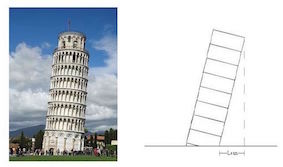
\includegraphics[width=0.8\linewidth]{src/images/chapter01/tower-of-pisa-image.jpg}
\caption{The Leaning Tower of Pisa and the measurement of the amount of lean\label{tower-of-pisa-image}}
\end{figure}
\hypertarget{p-89}{}%
Looking at the scatterplot in Figure 4. should convince us that there is a tight or strong relationship between these variables. Notice that we are only interested in the interval before the tower was stabilized. The points tend to slope upward to the right, so we say in this case there is a positive association between the variables. That is, both variables increase together. There does not appear to be any obvious consistent curvature; rather, the points seem to be increasing fairly steadily, so we conclude that the shape is linear. \\%
\begin{figure}
\centering
{
\begin{tikzpicture}
  \begin{axis}[
    scale only axis,
    width=\textwidth-45pt,
    height=8.5cm,
    xlabel = Year,
    ylabel = Lean (mm),
    xlabel near ticks,
    ylabel near ticks,
    xmin = 1974,
    xmax = 1988,
    ymin = 2960,
    ymax = 2976,
    xticklabel style={/pgf/number format/1000 sep=},
    xtick={1975,1976,...,1988},
    ytick={2962,2963,...,2976},
    axis y discontinuity=crunch,
    minor x tick num=0,
    minor y tick num=1,
    ]

    \addplot [thick, blue, mark=*, only marks] coordinates {
      (1975,2964.2)   (1976,2964.4)   (1977,2965.6)   (1978,2966.7)
      (1979,2967.3)   (1980,2968.8)   (1981,2969.6)   (1982,2969.8)
      (1983,2971.3)   (1984,2971.7)   (1985,2972.5)   (1986,2974.2)
      (1987,2975.7)
    };
  \end{axis}
\end{tikzpicture}
}
\caption{Lean versus Year\label{scatterplot-tower-of-pisa}}
\end{figure}
\hypertarget{p-90}{}%
Sometimes when we examine scatterplots we observe points that appear to stand out from the rest. These points may follow the general pattern of the data but are far removed from other points. Other times there are points that are inconsistent with the general trend. Such points may indicate errors in measurement or in plotting that need to be corrected, or they may indicate the presence of some factor that deserves special attention. Whatever the cause, we should look for, and attempt to explain, odd points, called \emph{outliers}, that do not appear to fit the general pattern of the scatterplot. \newpage%
\end{example}
\typeout{************************************************}
\typeout{Exercises 1.4 Exercises}
\typeout{************************************************}
\subsection*{Exercises}\hypertarget{exercises-3}{}
\addcontentsline{toc}{subsection}{Exercises}
\begin{divisionexercise}{1}\hypertarget{exercise-8}{}
\hypertarget{p-91}{}%
Comment on the important characteristics of the scatterplots provided below. The legends describe the variables on each axis. Consider the shape (linear or curved), whether the data describes an increasing or decreasing (positive or negative) relationship, any gaps, clusters, or outliers apparent in the data. Write a sentence or two to explain the story the data telling about the relationship between the two variables.%
\end{divisionexercise}%
\begin{sidebyside}{2}{0}{0}{0}
\begin{sbspanel}{0.5}
\resizebox{\linewidth}{!}{{
\begin{tikzpicture}
  \begin{axis}[
    xlabel = Average flight length (miles),
    ylabel = Average fuel use (gallons/hour),
    xlabel near ticks,
    ylabel near ticks,
    xmin = 0,
    xmax = 4000,
    ymin = 0,
    ymax = 4000,
    xticklabel style = {/pgf/number format/1000 sep=},
    xtick = {1000,2000,...,4000},
    ytick = {1000,2000,...,4000},
    minor x tick num = 1,
    minor y tick num = 1,
    ]

    \addplot [thick, blue, mark=*, only marks] coordinates {
      (386,639)   (386,804)   (453,849)   (612,731)   (699,877)
      (612,1130)  (692,1290)  (998,986)   (1240,1450) (1400,2210)
      (1540,1580) (1690,1500) (1740,1340) (1630,2220) (3140,3520)
    };
  \end{axis}
\end{tikzpicture}
}
}
\end{sbspanel}
\begin{sbspanel}{0.5}
\resizebox{\linewidth}{!}{{
\begin{tikzpicture}
  \begin{axis}[
    xlabel = Average temperature in March ($\text{C}^\circ$),
    ylabel = Day in April of first cherry blossoms,
    xlabel near ticks,
    ylabel near ticks,
    xmin = 0,
    xmax = 7,
    ymin = 0,
    ymax = 35,
    xtick = {1,2,...,7},
    ytick = {5,10,...,35},
    minor x tick num = 1,
    minor y tick num = 4,
    ]

    \addplot [thick, blue, mark=*, only marks] coordinates {
      (1.56,28) (2.65,19) (3.24,11) (3.7,17)  (3.84,14)
      (3.8,19)  (4.05,21) (4.09,17) (4.08,14) (4.05,13)
      (4.05,11) (4.25,14) (4.37,13) (4.53,10) (4.61,9)
      (4.71,14) (4.92,15) (4.95,9)  (5.01,7)  (5.13,11)
      (5.43,8)  (6.10,3)  (6.27,3)
    };
  \end{axis}
\end{tikzpicture}
}
}
\end{sbspanel}
\begin{sbscaption}{0.5}
\captionof{figure}{Plot 1\label{exercises-scatterplot-1}}
\end{sbscaption}
\begin{sbscaption}{0.5}
\captionof{figure}{Plot 2\label{exercises-scatterplot-2}}
\end{sbscaption}
\end{sidebyside}
\begin{figure}
\centering
{
\begin{tikzpicture}
  \begin{axis}[
    xlabel = Number of sqaures from GO,
    ylabel = Value of property,
    xlabel near ticks,
    ylabel near ticks,
    xmin = 0,
    xmax = 35,
    ymin = 0,
    ymax = 350,
    xtick = {5,10,...,35},
    ytick = {50,100,...,350},
    minor x tick num = 4,
    minor y tick num = 1,
    ]

    \addplot [thick, blue, mark=*, only marks] coordinates {
      (1,29)    (3,29)   (5,195)  (6,76)   (9,76)
      (9,98)    (11,124) (13,134) (14,123) (15,150)
      (16,192)  (17,172) (19,172) (20,194) (22,219)
      (24,218)  (25,242) (26,195) (27,265) (28,265)
      (30,136)  (30,289) (33,313)
    };
  \end{axis}
\end{tikzpicture}
}
\caption{Plot 3\label{exercises-scatterplot-3}}
\end{figure}
\begin{figure}
\centering
{
\begin{tikzpicture}
  \begin{axis}[
    scale only axis,
    width = \textwidth-45pt,
    height = 8.5cm,
    xlabel = Year,
    ylabel = Number of named Atlantic/Carribean storms,
    xlabel near ticks,
    ylabel near ticks,
    xmin = 1965,
    xmax = 2020,
    ymin = 0,
    ymax = 35,
    xticklabel style = {/pgf/number format/1000 sep=},
    xtick = {1960,1965,...,2015},
    ytick = {5,10,...,35},
    minor x tick num = 4,
    minor y tick num = 4,
    ]

    \addplot [thick, blue, mark=*, only marks] coordinates {
      (1982,12) (1983,5)  (1984,2)  (1985,13) (1986,11) (1987,5)
      (1988,6)  (1989,12) (1990,11) (1991,14) (1992,7)  (1993,6)
      (1994,7)  (1996,19) (1995,6)  (1997,13) (1998,7)  (1999,14)
      (2000,12) (2001,15) (2002,15) (2004,11) (2004,16) (2006,30)
      (2006,15) (2008,9)  (2009,15) (2010,16) (2011,8)  (2012,19)
      (2013,20) (2014,20) (2015,14) (2016,7)  (2017,10) (1966,10)
      (1967,7)  (1968,7)  (1969,19) (1970,10) (1971,13) (1972,6)
      (1973,7)  (1974,10) (1975,8)  (1976,9)  (1977,5)  (1978,12)
      (1979,8)  (1980,10)
    };
  \end{axis}
\end{tikzpicture}
}
\caption{Plot 4\label{exercises-scatterplot-4}}
\end{figure}
\begin{sidebyside}{2}{0}{0}{0}
\begin{sbspanel}{0.5}
\resizebox{\linewidth}{!}{{
\begin{tikzpicture}
  \begin{axis}[
    xlabel = Time object has been cooling (minutes),
    ylabel = Temperature ($\text{F}^\circ$),
    xlabel near ticks,
    ylabel near ticks,
    xmin = 0,
    xmax = 400,
    ymin = 0,
    ymax = 140,
    xtick = {100,200,...,400},
    ytick = {20,40,...,130},
    minor x tick num = 1,
    minor y tick num = 1,
    ]

    \addplot [thick, blue, mark=*, only marks] coordinates {
      (2.2,122.4)   (6.6,115.2)   (10.2,109.1)
      (37.2,85.9)   (51.9,76.2)   (65.2,66.7)
      (146.3,40.0)  (177.9,35.1)  (210.5,30.0)
      (332.3,22.4)  (390.3,19.2)  (245.3,25.3)
      (17.7,102.8)  (20.8,99.0)   (86.6,55.7)
      (300.2,22.9)  (128.4,42.6)
    };
  \end{axis}
\end{tikzpicture}
}
}
\end{sbspanel}
\begin{sbspanel}{0.5}
\resizebox{\linewidth}{!}{{
\begin{tikzpicture}
  \begin{axis}[
    xlabel = Minutes played for the 1987-88 Chicago Bulls,
    ylabel = Points scored,
    xlabel near ticks,
    ylabel near ticks,
    xmin = 0,
    xmax = 3600,
    ymin = 0,
    ymax = 3500,
    xtick = {600,1200,...,3600},
    ytick = {500,1000,...,3000},
    minor x tick num = 1,
    minor y tick num = 1,
    ]

    \addplot [thick, blue, mark=*, only marks] coordinates {
      (564.58,199.32)   (1035.30,279.41)
      (1482.11,608.75)  (1644.63,712.88)
      (1790.08,670.72)  (1871.41,696.98)
      (2184.95,853.57)  (2318.67,854.33)
      (2800.53,1123.68) (3295.27,312.96)
      (3295.2,3147.4)
    };
  \end{axis}
\end{tikzpicture}
}
}
\end{sbspanel}
\begin{sbscaption}{0.5}
\captionof{figure}{Plot 5\label{exercises-scatterplot-5}}
\end{sbscaption}
\begin{sbscaption}{0.5}
\captionof{figure}{Plot 6\label{exercises-scatterplot-6}}
\end{sbscaption}
\end{sidebyside}
\begin{figure}
\centering
{
\begin{tikzpicture}
  \begin{axis}[
    scale only axis,
      width=\textwidth-45pt,
      height= 6.5cm,
      xlabel = Year,
      ylabel = September Artic Sea Ice (million $\text{km}^2$,
      xlabel near ticks,
      ylabel near ticks,
      xmin = 1980,
      xmax = 2020,
      ymin = 3,
      ymax = 8,
      xticklabel style = {/pgf/number format/1000 sep=},
      xtick = {1980,1985,...,2020},
      ytick = {3,4,...,8},
      minor x tick num = 4,
      minor y tick num = 0,
      axis y discontinuity = crunch,
      ]

      \addplot [thick, blue, mark=*, only marks] coordinates {
        (1978,7.21) (1979,7.83) (1980,7.23) (1981,7.47) (1982,7.52)
        (1983,7.12) (1984,6.92) (1985,7.52) (1986,7.45) (1987,7.49)
        (1988,6.96) (1990,6.22) (1991,6.53) (1992,7.55) (1993,6.49)
        (1994,7.17) (1995,6.08) (1996,7.86) (1997,6.75) (1998,6.52)
        (1999,6.26) (2000,6.34) (2002,6.76) (2003,5.93) (2004,6.15)
        (2005,6.04) (2006,5.57) (2007,5.92) (2007,5.04) (2008,4.26)
        (2009,4.83) (2010,5.37) (2011,4.94) (2012,4.63) (2013,3.62)
        (2014,4.60) (2015,5.37) (2016,5.28) (2017,4.62) (2018,4.79)
      };
    \end{axis}
  \end{tikzpicture}
}
\caption{Plot 7\label{exercises-scatterplot-7}}
\end{figure}
\begin{figure}
\centering
{
\begin{tikzpicture}
  \begin{axis}[
    scale only axis,
    width=\textwidth-45pt,
    height= 6.5cm,
    xlabel = Year,
    ylabel = $text{CO}_2$ concentration in the atomsphere (parts per million),
    xlabel near ticks,
    ylabel near ticks,
    xmin = 2013,
    xmax = 2018,
    ymin = 390,
    ymax = 425,
    xticklabel style = {/pgf/number format/1000 sep=},
    xtick = {2013,2014,...,2018},
    ytick = {390,395,...,420},
    minor x tick num = 4,
    minor y tick num = 1,
    axis y discontinuity = crunch,
    ]

    \addplot [thick, blue, mark=*, only marks] coordinates {
      (2013.03,396.1) (2013.09,397.3) (2013.21,397.9) (2013.28,399.0)
      (2013.48,399.0) (2013.52,397.6) (2013.61,395.8) (2013.69,393.8)
      (2013.87,395.7) (2013.94,397.3) (2014.04,398.5) (2014.11,398.8)
      (2014.31,402.1) (2014.36,402.9) (2014.46,401.9) (2014.55,399.7)
      (2014.69,395.7) (2014.80,396.5) (2014.88,397.7) (2014.96,399.6)
      (2015.12,400.9) (2015.20,402.3) (2015.28,404.0) (2015.35,404.9)
      (2015.55,402.0) (2015.64,399.5) (2015.70,398.0) (2015.80,398.8)                                   (2015.96,402.5) (2016.01,403.2)   (2016.15,404.7)
      (2016.22,406.0) (2016.26,408.2) (2016.36,408.9) (2016.50,407.8)
      (2016.64,402.9) (2016.69,401.6) (2016.83,402.2) (2016.88,404.4)
      (2017.05,407.0) (2017.14,407.6) (2017.20,408.2) (2017.31,410.0)
      (2017.46,410.0) (2013.36,400.4) (2013.79,393.9) (2014.21,400.4)
      (2014.63,397.5) (2015.03,400.5) (2015.48,403.6) (2015.87,400.9)
      (2016.55,405.4) (2016.95,405.2) (2017.39,410.8)
    };
  \end{axis}
\end{tikzpicture}
}
\caption{Plot 8\label{exercises-scatterplot-8}}
\end{figure}
\begin{sidebyside}{2}{0}{0}{0}
\begin{sbspanel}{0.5}
\resizebox{\linewidth}{!}{{
\begin{tikzpicture}
  \begin{axis}[
    xlabel = Diameter (inches),
    ylabel = Weight Bells of St. Patrick’s Cathedral (pounds),
    xlabel near ticks,
    ylabel near ticks,
    xmin = 30,
    xmax = 70,
    ymin = 0,
    ymax = 6000,
    xtick = {30,35,...,70},
    ytick = {1000,2000,...,6000},
    minor x tick num = 1,
    minor y tick num = 4,
    axis x discontinuity = crunch,
    axis y discontinuity = crunch,
    ]

    \addplot [thick, blue, mark=*, only marks] coordinates {
      (29.5,1667.2) (31.5,1772.2) (34.1,1886.8) (34.9,1934.4)
      (36.6,1925.3) (38.1,2068.1) (42.1,2373.0) (47.1,2820.7)
      (49.4,3058.8) (55.0,3829.9) (61.9,5266.5)
    };
  \end{axis}
\end{tikzpicture}
}
}
\end{sbspanel}
\begin{sbspanel}{0.5}
\resizebox{\linewidth}{!}{{
\begin{tikzpicture}
  \begin{axis}[
    xlabel = Outside temperature ($\text{C}^\circ$),
    ylabel = Gas consumption (1000 cubic feet),
    xlabel near ticks,
    ylabel near ticks,
    xmin = -1,
    xmax = 6,
    ymin = 3,
    ymax = 5,
    xtick = {-1,0,...,5},
    ytick = {3,4,...,5},
    minor x tick num = 0,
    minor y tick num = 1,
    axis y discontinuity=crunch,
    ]

    \addplot [thick, blue, mark=*, only marks] coordinates {
      (-0.70,4.95)  (-0.29,4.96)  (0.01,4.20)   (0.81,4.74)
      (1.01,4.87)   (1.41,4.09)   (1.51,4.30)   (1.65,4.30)
      (2.32,4.21)   (2.53,3.54)   (2.54,4.08)   (3.11,3.21)
      (3.93,3.98)   (4.02,3.77)   (4.01,3.55)   (4.20,3.54)                                  (4.32,3.53)   (4.63,3.77)   (4.72,3.53)   (4.91,3.42)
    };
  \end{axis}
\end{tikzpicture}
}
}
\end{sbspanel}
\begin{sbscaption}{0.5}
\captionof{figure}{Plot 9\label{exercises-scatterplot-9}}
\end{sbscaption}
\begin{sbscaption}{0.5}
\captionof{figure}{Plot 10\label{exercises-scatterplot-10}}
\end{sbscaption}
\end{sidebyside}
\begin{figure}
\centering
{
\begin{tikzpicture}
  \begin{axis}[
    scale only axis,
    width = \textwidth-45pt,
    height = 8.5cm,
    xlabel = Year,
    ylabel = Average difference in ocean temperature,
    xlabel near ticks,
    ylabel near ticks,
    xmin = 1940,
    xmax = 2020,
    ymin = -0.5,
    ymax = 1,
    xticklabel style = {/pgf/number format/1000 sep=},
    xtick = {1940,1950,...,2020},
    ytick = {-1,-0.5,...,2},
    minor x tick num = 4,
    minor y tick num = 1,
    ]

    \addplot [thick, blue, mark=*, only marks] coordinates {
      (1950,-0.2993)  (1954,-0.2740)  (1960,-0.1270)  (1965,-0.2198)
      (1970,-0.0764)  (1975,-0.1620)  (1981,0.2070)   (1985,-0.0076)
      (1989,0.3971)   (1995,0.4153)   (2000,0.3332)   (2005,0.6449)
      (2010,0.6916)   (2016,0.8853)
    };
  \end{axis}
\end{tikzpicture}
}
\caption{Plot 11\label{exercises-scatterplot-11}}
\end{figure}
\begin{figure}
\centering
{
\begin{tikzpicture}
  \begin{axis}[
    xlabel = Weight of dog (pounds),
    ylabel = Number of cups of Aplo dog food,
    xlabel near ticks,
    ylabel near ticks,
    xmin = 0,
    xmax = 200,
    ymin = 0,
    ymax = 10,
    xtick = {0,50,...,200},
    ytick = {1,2,...,10},
    minor x tick num = 1,
    minor y tick num = 0,
    ]

    \addplot [thick, blue, mark=*, only marks] coordinates {
      (7.2,1)   (19.3,2)  (36.2,3)  (57.4,4)
      (80.2,5)  (102.6,6) (131.3,7) (159.4,8)
      (191.3,9)
    };
  \end{axis}
\end{tikzpicture}
}
\caption{Plot 12\label{exercises-scatterplot-12}}
\end{figure}
\typeout{************************************************}
\typeout{Section 1.5 Linear Models}
\typeout{************************************************}
\section[{Linear Models}]{Linear Models}\label{chapter01-section05}
\hypertarget{p-92}{}%
When you examined the scatterplots in the exercises in the last section, you should have noticed several graphs with points that stand apart from the others. In \hyperref[exercises-scatterplot-1]{Figure~8}, the point in the upper right corner represents an airplane with an exceptionally high number of seats and exceptionally high fuel consumption (Boing 747). Cover this points with your finger and use the other points to predict fuel consumption for a plane with 400 seats. Do you consider this point to follow the general trend of the other data points? In \hyperref[exercises-scatterplot-2]{Figure~9}, there is a point in the upper left corner that fits the general trend of the data but is noticeably removed from the other points. This point represents a year in which the average March temperature was unusually low and the cherry blossoms did not appear until late in April. These points differ from the outlier found in \hyperref[exercises-scatterplot-6]{Figure~13}. The outlier represents Michael Jordan, the legendary player who led the Chicago Bulls to six NBA Championships. Jordan had the highest playing time but his playing time is not inconsistent with that of the other players. This point is an outlier because of the very high number of points scored. Michael Jordan does not have statistics that follow the general pattern of the other players on the Bulls.%
\par
\hypertarget{p-93}{}%
When a relationship is suggested by a scatterplot, we usually want to describe it mathematically by finding an equation that summarizes the way the two variables are related. Such an equation is another example of a mathematical model. When we discussed mathematical models at the beginning of the chapter, we pointed out that a good model simplifies the phenomenon it represents and gives us the ability to predict. If we can find the equation of a curve that closely “fits” a scatterplot, we can focus on the important characteristics of the relationship between the variables without the clutter of a scatterplot. We can also use this equation to predict the values of one variable for specific values of the other variable. Sometimes we use the model to \emph{interpolate}, or estimate new values among data values and sometimes we use the model to \emph{extrapolate}, or predict values outside the region of the data. To extrapolate, we must have good reason to believe that the pattern seen in the data continues.%
\par
\hypertarget{p-94}{}%
To obtain an equation to model the Leaning Tower of Pisa data during the period in which the tower was leaning, you could sketch a line that passes through the data and follows the general path of the data. What is the equation of the line that best fits this data? The process of fitting a linear model to a set of data is an important aspect of data analysis. With the help of graphing calculators or computers, we can quickly fit a line to a given set of data. For the moment we will just estimate the location of the linear model to demonstrate how you can use this line. In \hyperref[tower-of-pisa-linear-model]{Figure~1} we show a line through the data of our scatterplot.%
\begin{figure}
\centering
{
\begin{tikzpicture}
  \begin{axis}[
    scale only axis,
    width=\textwidth-45pt,
    height=8.5cm,
    xlabel = Year,
    ylabel = Lean (mm),
    xlabel near ticks,
    ylabel near ticks,
    xmin = 1974,
    xmax = 1988,
    ymin = 2960,
    ymax = 2976,
    xticklabel style = {/pgf/number format/1000 sep=},
    xtick = {1975,1976,...,1988},
    ytick = {2962,2963,...,2976},
    axis y discontinuity = crunch,
    minor x tick num = 0,
    minor y tick num = 1,
    clip mode = individual,
    ]

    \addplot [thick, blue, mark=*, only marks] coordinates {
      (1975,2964.2)   (1976,2964.4)   (1977,2965.6)   (1978,2966.7)
      (1979,2967.3)   (1980,2968.8)   (1981,2969.6)   (1982,2969.8)
      (1983,2971.3)   (1984,2971.7)   (1985,2972.5)   (1986,2974.2)
      (1987,2975.7)
    };
    \addplot [thick, red, mark=none, samples=200] coordinates {(1975,2963.9) (1987,2974.9)};
  \end{axis}
\end{tikzpicture}
}
\caption{Leaning Tower of Pisa with linear model\label{tower-of-pisa-linear-model}}
\end{figure}
\hypertarget{p-95}{}%
Notice how the line follows the pattern of the points in this scatterplot. Some of the points are above the line, some are below, but they are all close to the line. Since the data points are closely following the path of our line, we can conclude that the relationship between these variables is strong and can feel very confident that our line does a good job of describing this particular phenomenon. We expect the same trend to continue into the near future, so we would also feel confident in using our model to extrapolate, or to predict the value of the lean in future years.%
\par
\hypertarget{p-96}{}%
How close do the points have to be to consider the model good? Think back to Example 1 and re-examine the scatterplot in \hyperref[scatterplot-tower-of-pisa]{Figure~7}. Try to sketch a line that follows the path of this data. \hyperref[tower-of-pisa-linear-model]{Figure~1} shows one possible line that could be used to model from the data of Francis Galton, one of the founders of modern-day statistics. In the late 1800’s, Galton compared the height, in inches, of 952 fathers with the height at maturity of his firstborn son. It was this study and others like it that led Galton to develop the method of linear regression and to define the standard deviation as a measure of spread. You will notice that most of the data points are not close to the line. This does not mean that a linear model is inappropriate. There is no evidence at all of any curvature in the data, so a linear equation is indeed appropriate. There is a great deal of variation in the heights of the sons, and so our model needs to acknowledge this in some way. The issue of closeness is relative and depends on the particular variables and the size of their values. \begin{figure}
\centering
{
\begin{tikzpicture}
  \begin{axis}[
    xlabel = Parent Height,
    ylabel = Child Height,
    xlabel near ticks,
    ylabel near ticks,
    xmin = 60,
    xmax = 75,
    ymin = 60,
    ymax = 75,
    xtick = {60,61,...,75},
    ytick = {60,61,...,75},
    clip mode = individual,
    ]
    \addplot [thick, blue, mark=*, only marks] coordinates {
    (62.56,67.06) (62.56,65.96) (62.58,64.46) (62.90,62.95) (63.42,66.08) (65.26,66.96) (66.18,63.90)
    (62.85,68.48) (63.01,67.38) (63.13,64.98) (63.34,69.50) (63.44,64.25) (65.00,68.88) (66.07,64.39)
    (63.58,62.78) (63.58,62.13) (63.61,67.38) (63.60,66.24) (63.83,66.28) (65.12,68.92) (65.75,66.18)
    (63.81,65.02) (63.94,68.88) (63.93,67.38) (63.97,66.07) (63.89,64.57) (65.02,70.50) (65.91,65.94)
    (63.91,63.96) (64.03,64.12) (64.15,63.51) (64.25,62.90) (64.37,61.96) (65.12,69.36) (65.83,66.59)
    (64.54,61.27) (64.18,67.09) (64.44,63.59) (64.48,67.33) (64.44,65.95) (65.26,69.24) (65.96,66.83)
    (64.68,64.89) (64.79,64.16) (64.62,63.67) (64.70,62.69) (64.80,62.69) (65.26,69.00) (65.94,67.08)
    (64.91,62.97) (64.93,63.54) (64.70,64.28) (64.75,65.09) (64.64,65.09) (65.08,71.32) (65.85,67.57)
    (64.61,67.17) (64.75,66.92) (64.79,67.94) (64.83,68.71) (64.88,69.57) (65.39,71.68) (65.69,68.79)
    (64.67,70.22) (65.02,68.31) (64.87,67.00) (64.89,66.47) (64.95,65.05) (65.47,72.13) (65.61,70.34)
    (64.95,64.76) (65.01,64.32) (65.09,64.11) (65.23,63.54) (65.29,62.93) (65.60,71.31) (65.78,70.13)
    (65.58,61.30) (65.48,63.26) (65.32,63.99) (65.18,64.84) (65.10,65.90) (65.45,70.42) (65.88,69.56)
    (65.10,66.15) (65.18,66.39) (65.10,66.80) (64.99,66.88) (65.20,66.92) (65.51,70.05) (65.88,69.28)
    (65.41,68.10) (65.34,67.65) (65.51,67.94) (65.42,67.16) (65.53,67.00) (65.71,66.96) (65.79,68.63)
    (65.75,66.55) (65.53,66.35) (65.32,66.06) (65.57,65.90) (65.32,65.37) (65.48,65.49) (65.88,68.63)
    (65.61,65.57) (65.79,65.33) (65.50,65.05) (65.71,64.43) (65.68,63.99) (65.82,61.71) (65.93,62.07)
    (65.94,68.34) (66.02,67.40) (66.10,66.95) (66.04,66.43) (66.10,66.14) (66.18,66.47) (66.04,65.90)
    (66.12,65.73) (66.26,65.41) (66.44,63.94) (66.54,63.37) (66.56,63.09) (66.68,62.88) (66.72,61.58)
    (66.93,62.47) (66.89,63.08) (66.83,63.08) (66.38,65.73) (66.32,65.73) (66.28,66.18) (66.34,66.22)
    (66.55,66.54) (66.26,66.79) (66.34,66.95) (66.43,67.24) (66.18,67.20) (66.22,67.48) (66.16,67.85)
    (66.12,68.18) (66.20,68.26) (66.10,68.75) (66.14,69.15) (66.14,69.72) (66.12,70.09) (66.21,70.17)
    (66.55,69.52) (66.35,68.50) (66.18,68.42) (66.51,68.50) (66.51,68.17) (66.45,67.77) (66.47,66.02)
    (67.26,62.02) (67.07,63.69) (67.12,64.14) (66.91,64.18) (66.99,64.30) (67.04,64.71) (66.93,64.87)
    (66.75,65.20) (66.91,65.52) (66.79,65.69) (66.75,65.89) (66.65,66.06) (66.73,66.26) (66.81,66.34)
    (66.90,66.34) (66.81,66.83) (66.81,67.11) (66.88,67.28) (66.79,67.40) (66.69,67.93) (66.65,68.17)
    (66.76,68.21) (66.88,68.05) (66.86,68.54) (66.76,68.54) (66.76,68.82) (66.65,68.82) (66.76,69.19)
    (66.76,69.39) (66.76,69.84) (66.90,69.88) (66.82,70.12) (66.78,70.53) (66.96,70.53) (66.74,71.06)
    (66.78,72.00) (66.86,71.55) (67.81,66.37) (66.86,72.28) (67.07,71.95) (67.19,71.55) (67.21,71.26)
    (67.15,70.69) (67.02,69.59) (66.90,69.19) (67.02,68.98) (67.15,69.31) (67.11,69.67) (67.21,68.98)
    (67.08,68.86) (67.08,68.70) (67.10,67.97) (67.02,67.60) (67.02,67.31) (67.10,67.11) (66.96,66.83)
    (67.14,66.54) (67.14,65.97) (67.08,65.93) (67.14,65.56) (67.14,65.24) (67.30,65.12) (67.42,65.40)
    (67.47,65.64) (67.26,65.77) (67.46,64.46) (67.38,64.18) (67.22,64.42) (67.30,63.12) (67.62,62.22)
    (68.07,61.94) (67.71,63.08) (67.61,63.65) (67.73,63.61) (67.69,64.22) (67.75,64.71) (67.65,64.71)
    (67.63,64.87) (67.69,65.56) (67.73,65.76) (67.67,66.05) (67.59,66.05) (67.49,65.85) (67.45,66.17)
    (67.57,66.46) (67.53,66.62) (67.45,66.66) (67.39,66.62) (67.32,66.38) (67.47,66.99) (67.47,67.23)
    (67.41,67.23) (67.41,67.76) (67.31,67.84) (67.25,67.96) (67.43,68.17) (67.25,68.33) (67.41,68.53)
    (67.35,68.66) (67.45,68.90) (67.37,68.94) (67.47,69.14) (67.49,69.47) (67.39,69.67) (67.27,69.59)
    (67.23,69.76) (67.27,70.00) (67.29,70.32) (67.39,70.00) (67.15,72.48) (67.23,72.20) (67.31,71.91)
    (67.37,71.71) (67.42,71.59) (67.46,71.30) (67.45,70.69) (67.52,70.45) (67.64,70.12) (67.72,69.75)
    (67.74,69.47) (67.62,69.35) (67.68,69.18) (67.53,68.86) (67.74,68.73) (67.78,68.65) (67.84,68.20)
    (67.76,68.29) (67.63,68.41) (67.57,68.21) (67.55,67.96) (67.69,67.80) (67.51,67.60) (67.61,67.47)
    (67.71,67.23) (67.67,67.07) (67.67,66.94) (67.67,66.82) (67.67,66.58) (67.75,66.46) (67.88,66.09)
    (68.00,65.92) (67.85,65.44) (67.77,65.48) (68.08,65.44) (68.04,65.03) (68.02,64.74) (67.89,64.38)
    (67.91,63.97) (67.81,63.97) (68.06,63.52) (68.03,62.95) (68.38,62.67) (68.26,63.52) (68.14,63.69)
    (68.32,63.93) (68.40,64.21) (68.26,64.29) (68.36,64.54) (68.45,64.66) (68.45,65.03) (68.43,65.31)
    (68.37,65.47) (68.22,65.68) (68.08,65.76) (68.08,66.33) (68.02,66.33) (67.92,66.62) (68.08,66.86)
    (68.02,67.15) (67.90,67.43) (67.86,67.55) (67.98,67.67) (68.10,67.31) (68.12,67.59) (68.08,67.80)
    (68.08,68.24) (67.96,68.73) (67.88,68.86) (67.82,69.06) (68.64,69.18) (67.82,69.87) (67.72,70.48)
    (67.72,70.61) (67.70,70.93) (67.62,70.97) (67.54,71.99) (67.50,72.28) (68.03,71.70) (67.93,71.46)
    (67.88,71.34) (67.92,70.85) (68.09,70.52) (68.03,69.91) (68.02,69.63) (68.02,69.18) (68.15,68.77)
    (67.94,69.06) (67.84,69.34) (68.19,68.28) (68.08,68.20) (68.39,68.00) (68.25,67.79) (68.31,67.51)
    (68.29,67.22) (68.41,67.31) (68.41,67.18) (68.39,66.78) (68.33,66.65) (68.24,66.17) (68.35,66.13)
    (68.53,65.64) (68.61,65.27) (68.73,64.86) (68.75,63.93) (68.65,63.52) (68.98,63.96) (68.89,64.21)
    (68.90,64.62) (68.71,64.41) (68.82,65.51) (68.63,65.68) (68.69,65.84) (68.65,66.08) (68.78,66.04)
    (68.78,66.37) (68.74,66.57) (68.69,66.57) (68.63,66.45) (68.51,66.29) (68.41,66.33) (68.49,67.02)
    (68.70,67.02) (68.72,67.18) (68.68,67.30) (68.72,67.51) (68.70,67.79) (68.55,67.79) (68.72,68.04)
    (68.57,68.24) (68.31,68.49) (68.39,68.61) (68.29,68.81) (68.19,69.14) (68.27,69.30) (68.13,69.71)
    (68.17,70.12) (68.31,69.71) (68.33,69.63) (68.39,69.42) (68.49,69.26) (68.49,68.69) (68.64,68.44)
    (68.74,68.24) (68.86,67.95) (68.88,67.67) (68.88,67.30) (68.88,66.98) (68.78,66.77) (69.04,65.96)
    (69.24,65.43) (69.31,65.18) (69.43,65.18) (69.65,64.98) (69.26,64.45) (69.26,64.08) (69.14,64.00)
    (69.32,62.86) (70.14,62.94) (69.59,63.76) (69.73,63.88) (69.63,64.04) (69.51,64.00) (69.57,64.29)
    (69.75,64.28) (69.55,65.75) (69.49,65.87) (69.51,66.20) (69.37,66.20) (69.33,66.32) (69.16,66.16)
    (69.10,66.45) (69.02,66.57) (69.23,66.85) (69.02,67.06) (68.98,67.30) (68.98,67.99) (68.90,68.16)
    (68.78,68.69) (68.64,69.91) (68.46,70.24) (68.31,70.60) (68.17,70.89) (68.25,71.05) (68.25,71.46)
    (68.17,71.66) (68.11,71.87) (68.01,71.87) (67.97,72.64) (68.07,73.21) (68.17,72.84) (68.11,72.15)
    (68.32,71.99) (68.48,71.78) (68.48,71.54) (68.38,71.54) (68.46,71.05) (68.52,70.64) (68.72,70.64)
    (68.86,70.23) (68.99,69.91) (68.99,69.62) (68.88,69.62) (68.76,69.42) (69.05,69.05) (69.11,69.17)
    (69.13,68.77) (69.07,71.17) (68.96,68.77) (68.96,68.40) (69.17,68.03) (69.25,68.36) (69.31,67.75)
    (69.39,67.75) (69.45,67.58) (69.53,67.26) (69.45,67.26) (69.17,67.42) (69.25,67.18) (69.41,66.97)
    (69.61,66.81) (69.80,66.69) (69.80,66.08) (70.61,64.81) (70.15,66.72) (69.74,67.34) (69.60,67.70)
    (69.76,67.70) (69.84,68.03) (69.78,68.48) (69.54,68.89) (69.31,68.97) (69.23,69.42) (69.07,69.78)
    (69.17,70.03) (69.01,70.35) (69.13,70.43) (69.01,70.68) (68.82,70.76) (68.78,71.17) (68.60,71.29)
    (68.62,71.62) (68.50,72.07) (68.70,72.23) (68.56,72.23) (68.44,73.33) (68.93,74.42) (69.12,74.30)
    (69.36,73.97) (69.48,74.14) (69.52,73.32) (69.75,73.48) (69.38,72.83) (69.20,72.96) (68.95,73.20)
    (68.95,72.39) (69.07,72.31) (69.05,72.14) (68.95,72.06) (68.87,72.19) (68.87,71.94) (68.76,71.78)
    (69.07,71.45) (69.19,71.25) (69.25,71.21) (69.36,71.45) (69.25,71.61) (69.19,71.86) (69.40,71.86)
    (69.38,72.26) (69.50,71.21) (69.50,70.92) (69.43,69.21) (69.25,70.96) (69.42,70.64) (69.44,70.43)
    (69.29,70.43) (69.25,69.90) (69.46,69.58) (69.58,69.78) (69.66,69.49) (69.66,69.21) (69.82,68.96)
    (69.74,68.92) (69.90,68.56) (70.03,68.56) (70.13,68.43) (70.03,68.03) (70.02,67.62) (70.59,66.23)
    (70.96,66.15) (71.19,65.82) (71.64,65.09) (71.39,66.27) (70.92,66.76) (70.60,66.84) (70.98,67.08)
    (71.05,67.21) (71.11,67.21) (71.58,67.00) (71.23,68.02) (71.13,67.86) (70.72,68.02) (70.88,68.31)
    (70.78,68.51) (70.72,68.63) (70.84,68.79) (70.46,68.23) (70.21,68.43) (70.29,68.80) (70.52,68.80)
    (70.66,69.04) (70.50,69.29) (70.56,69.61) (70.38,69.61) (70.35,69.08) (70.29,69.33) (70.17,69.00)
    (70.13,69.49) (69.99,69.74) (70.09,69.90) (70.25,69.86) (70.36,69.90) (70.52,70.10) (70.27,70.14)
    (70.09,70.35) (70.15,70.83) (70.01,70.67) (69.76,70.63) (69.68,70.51) (69.66,70.27) (69.78,69.94)
    (69.81,70.96) (69.91,70.96) (69.93,71.32) (69.85,71.32) (69.64,71.53) (69.64,71.77) (69.73,71.77)
    (69.64,72.14) (69.87,72.34) (69.79,72.67) (70.01,72.63) (70.12,74.25) (70.16,73.32) (70.46,72.66)
    (70.46,72.42) (70.63,72.34) (70.60,71.89) (70.44,71.65) (70.40,71.48) (70.38,71.36) (70.48,71.08)
    (70.44,70.67) (70.32,70.59) (70.72,69.57) (70.89,69.32) (70.89,69.32) (71.09,69.32) (71.38,68.59)
    (71.76,68.06) (71.32,69.08) (71.34,69.52) (71.34,70.09) (71.21,70.09) (70.93,70.10) (70.97,70.30)
    (70.91,70.63) (70.89,70.87) (70.75,71.85) (70.83,72.13) (70.91,72.13) (70.55,73.68) (70.83,73.68)
    (71.04,74.21) (71.12,74.21) (71.24,70.91) (71.24,70.58) (71.48,71.15) (71.75,70.01) (71.75,69.40)
    (71.85,68.83) (72.05,68.79) (72.68,67.52) (71.89,70.01) (71.95,70.62) (71.97,71.68) (71.67,71.88)
    (71.81,72.25) (71.65,72.41) (71.81,72.94) (71.57,73.92) (72.04,73.34) (71.96,74.57) (72.43,73.71)
    (72.61,71.22) (72.69,70.70) (72.81,70.33) (72.67,69.47) (72.83,71.71) (72.83,72.12) (72.59,74.11)
    (72.94,74.64) (73.35,73.38) (73.35,73.17) (73.63,72.03) (73.92,73.37)
    };
    \addplot [ultra thick, red, mark=none, samples=200] coordinates {
    (61.23,65.57) (74.95,71.38)
    };
  \end{axis}
\end{tikzpicture}
}
\caption{Galton's scatterplot with a linear model\label{galtons-plot-data}}
\end{figure}
%
\typeout{************************************************}
\typeout{Exercises 1.5 Exercises}
\typeout{************************************************}
\subsection*{Exercises}\hypertarget{exercises-4}{}
\addcontentsline{toc}{subsection}{Exercises}
\begin{divisionexercise}{1}\hypertarget{exercise-9}{}
\hypertarget{p-97}{}%
In Iowa City, Iowa, the monthly utility bill provides the customer with information about the daily cost of gas and electricity as well as the average temperature during the month. The following information has been taken from a household in Iowa City for the months of August through September. (Source: Kathleen M. Heid, Algebra in a Technological World, Curriculum and Evaluation Standards for School Mathematics Addenda Series, NCTM, Reston, VA, 1995.) \leavevmode%
\begin{figure}
\centering
\begin{tabular}{lllllllll}\hrulemedium
Month&\multicolumn{1}{c}{Aug.}&\multicolumn{1}{c}{Sept.}&\multicolumn{1}{c}{Oct.}&\multicolumn{1}{c}{Nov.}&\multicolumn{1}{c}{Dec.}&\multicolumn{1}{c}{Jan.}&\multicolumn{1}{c}{Feb.}&\multicolumn{1}{c}{Mar.}\tabularnewline\hrulemedium
Avg. Temp.&\multicolumn{1}{c}{\(70\)}&\multicolumn{1}{c}{\(69\)}&\multicolumn{1}{c}{\(58\)}&\multicolumn{1}{c}{\(44\)}&\multicolumn{1}{c}{\(31\)}&\multicolumn{1}{c}{\(23\)}&\multicolumn{1}{c}{\(27\)}&\multicolumn{1}{c}{\(27\)}\tabularnewline\hrulemedium
Avg. Daily Cost (gas)&\multicolumn{1}{c}{\(0.35\)}&\multicolumn{1}{c}{\(0.38\)}&\multicolumn{1}{c}{\(0.78\)}&\multicolumn{1}{c}{\(1.41\)}&\multicolumn{1}{c}{\(1.86\)}&\multicolumn{1}{c}{\(1.94\)}&\multicolumn{1}{c}{\(1.97\)}&\multicolumn{1}{c}{\(1.76\)}\tabularnewline\hrulemedium
Avg. Daily Cost (electricity)&\multicolumn{1}{c}{\(0.98\)}&\multicolumn{1}{c}{\(0.78\)}&\multicolumn{1}{c}{\(0.82\)}&\multicolumn{1}{c}{\(0.77\)}&\multicolumn{1}{c}{\(0.86\)}&\multicolumn{1}{c}{\(0.65\)}&\multicolumn{1}{c}{\(0.80\)}&\multicolumn{1}{c}{\(0.73\)}\tabularnewline\hrulemedium
\end{tabular}
\caption{Heating Bill Data\label{heating-bill-data}}
\end{figure}
 \leavevmode%
\begin{enumerate}[label=(\alph*)]
\item\hypertarget{li-10}{}Make two scatterplots of the data. One scatterplot should show the average cost of gas as the dependent variable and the average temperature as the independent variable. The other scatterplot should show average cost of electricity as the dependent variable and the average temperature as the independent variable.%
\item\hypertarget{li-11}{}Describe the relationship between each pair of variables.%
\item\hypertarget{li-12}{}Sketch a free-hand line through each set of data and find the equation of each line. Use the equations to estimate the gas and the electric bill if the average temperature for this February was 19 degrees.%
\item\hypertarget{li-13}{}How confident are you in the predictions you made in part c? Explain your answer.%
\end{enumerate}
%
\end{divisionexercise}%
\begin{divisionexercise}{2}\hypertarget{exercise-10}{}
\hypertarget{p-98}{}%
Comment on the important characteristics of the scatterplots provided below. The legends describe the variables on each axis. Consider the shape (linear or curved), whether the data describes an increasing or decreasing (positive or negative) relationship, any gaps, clusters, or outliers apparent in the data. Write a sentence or two to explain the story the data telling about the relationship between the two variables.%
\leavevmode%
\begin{enumerate}[label=(\alph*)]
\item\hypertarget{li-14}{}The scatterplot below shows the length (in cm) of a pendulum and the period. Period is the time in seconds it takes to complete one oscillation, returning to the starting position. The ordered pairs are (length, time). \leavevmode%
\begin{figure}
\centering
{
\begin{tikzpicture}
  \begin{axis}[
    xlabel = Length (cm),
    ylabel = Time (seconds),
    xlabel near ticks,
    ylabel near ticks,
    xmin = 0,
    xmax = 50,
    ymin = 0,
    ymax = 1.5,
    xtick = {0,10,...,50},
    ytick = {0.2,0.4,...,1.4},
    minor x tick num = 1,
    minor y tick num = 1,
    ]

    \addplot [thick, blue, mark=*, only marks] coordinates {
      (7.3,0.4)   (9.6,0.51)   (11.7,0.61)   (13.9,0.68)   (16,0.73)
      (17.7,0.8)  (20.2,0.87)  (25.3,1)      (26.4,1.02)   (28.2,1.09)
      (32.3,1.14) (35.6,1.28)  (38.6,1.28)   (42.5,1.32)   (45.3,1.33)
    };
  \end{axis}
\end{tikzpicture}
}
\caption{\label{pendulum-data}}
\end{figure}
%
\item\hypertarget{li-15}{}The scatterplot below shows the horsepower of the engine for a variety of different cars and the number of miles per gallon an owner might expect to get driving. Source: \href{https://www.statcrunch.com/5.0/viewresult.php?resid=1878105}{StatCrunch}. \begin{figure}
\centering
{
\begin{tikzpicture}
  \begin{axis}[
    xlabel = Engine Horsepower,
    ylabel = Miles per Hour,
    xlabel near ticks,
    ylabel near ticks,
    xmin = 40,
    xmax = 160,
    ymin = 10,
    ymax = 40,
    xtick = {40,60,...,160},
    ytick = {10,15,...,40},
    minor x tick num = 1,
    minor y tick num = 1,
    ]

    \addplot [thick, blue, mark=*, only marks] coordinates {
    (64.7,33.8)   (64.5,31.7)   (67.9,30.2)   (67.9,29.6)   (70.1,34.4)   (71.0,32.2)
    (71.0,31.5)   (74.9,31.0)   (79.9,35.4)   (77.7,30.6)   (80.1,27.5)   (90.0,33.5)
    (85.1,21.1)   (88.0,26.7)   (89.7,28.5)   (94.5,27.8)   (96.9,27.3)   (96.4,22.5)
    (102.7,20.4)  (104.3,21.0)  (108.8,22.2)  (110.1,21.8)  (110.1,18.9)  (114.8,29.2)
    (115.2,26.8)  (115.2,22.2)  (119.7,18.4)  (124.7,19.6)  (125.2,17.3)  (128.0,18.0)
    (129.5,17.4)  (133.2,16.5)  (134.7,18.4)  (137.8,17.0)  (141.5,16.1)  (149.8,18.7)
    (155.0,17.2)
    };
  \end{axis}
\end{tikzpicture}
}
\caption{\label{horsepower-data}}
\end{figure}
%
\item\hypertarget{li-16}{}The scatterplots below show the number of touchdowns and interceptions thrown vs the quarterback ratings for NFL quarterbacks during the 2016 season. Source: \emph{The World Almanac and Book of Facts 2017}. \begin{figure}
\centering
\begin{sidebyside}{2}{0}{0}{0}
\begin{sbspanel}{0.5}
\resizebox{\linewidth}{!}{{
\begin{tikzpicture}
  \begin{axis}[
    xlabel = Touchdowns Thrown,
    ylabel = Quarterback Rating,
    xlabel near ticks,
    ylabel near ticks,
    xmin = 5,
    xmax = 40,
    ymin = 70,
    ymax = 120,
    xtick = {10,20,...,40},
    ytick = {80,90,...,120},
    minor x tick num = 1,
    minor y tick num = 1,
    ]
    \addplot [thick, blue, mark=*, only marks] coordinates {
    (12.0,94.5)   (14.0,89.1)   (19.0,91.8)   (20.1,100.9)  (20.1,96.4)   (20.9,95.8)
    (21.2,93.1)   (21.1,89.8)   (24.0,89.2)   (25.2,108.4)  (29.1,103.4)  (29.1,94.6)
    (31.1,88.4)   (31.1,93.5)   (32.1,91.7)   (32.2,98.6)   (32.2,102.7)  (33.9,112.8)
    (35.0,106.7)  (36.2,104.1)  (35.0,100.8)  (35.0,94.7)   (35.1,89.0)
    };
  \end{axis}
\end{tikzpicture}
}
}
\end{sbspanel}
\begin{sbspanel}{0.5}
\resizebox{\linewidth}{!}{{
\begin{tikzpicture}
  \begin{axis}[
    xlabel = Interceptions Thrown,
    ylabel = Quarterback Rating,
    xlabel near ticks,
    ylabel near ticks,
    xmin = 0,
    xmax = 20,
    ymin = 70,
    ymax = 120,
    xtick = {5,10,...,20},
    ytick = {80,90,...,120},
    minor x tick num = 1,
    minor y tick num = 1,
    ]
    \addplot [thick, blue, mark=*, only marks] coordinates {
    (4.0,94.0)    (6.2,101.0)   (7.1,108.2) (7.1,104.0)   (7.1,96.6)  (7.1,91.8)
    (8.1,112.2)   (8.1,93.6)    (9.0,89.0)  (10.1,100.9)  (10.2,92.4) (11.0,106.3)
    (11.0,103.3)  (11.1,102.1)  (11.1,93.4) (16.0,95.5)   (16.0,89.9) (18.0,88.5)
    (12.1,88.5)   (13.0,98.1)   (13.0,94.3) (13.0,91.5)   (14.1,94.5) (15.0,88.1)
    };
  \end{axis}
\end{tikzpicture}
}
}
\end{sbspanel}
\end{sidebyside}
\caption{\label{tds-qbr-int-data}}
\end{figure}
%
\end{enumerate}
\end{divisionexercise}%
\begin{divisionexercise}{3}\hypertarget{exercise-11}{}
\hypertarget{p-99}{}%
Characteristics of different Boeing aircraft flying in the US are given below.%
\leavevmode%
\begin{enumerate}[label=(\alph*)]
\item\hypertarget{li-17}{}From the descriptions in the table, try to predict which variables have a linear relationship. Check two of your predictions by creating scatterplots of the data. Were your predictions reasonable?%
\item\hypertarget{li-18}{}New data from old: Compute a data set that represents:%
%
\begin{enumerate}[label=\roman*.]
\item\hypertarget{li-19}{}the average times of a flight by computing \(\displaystyle \left( {\frac{{{\rm{Length}}\left( m \right)}}{{{\rm{Speed}}\left( {\frac{m}{{hr}}} \right)}}} \right)\)%
\item\hypertarget{li-20}{}the average cost per mile by computing \(\displaystyle \left( {\frac{{{\text{Cost}}\left( {\frac{\$ }{{hr}}} \right)}}{{{\text{Speed}}\left( {\frac{m}{{hr}}} \right)}}} \right)\)%
\item\hypertarget{li-21}{}the average cost per passenger by computing \(\displaystyle \left( {\frac{{{\rm{Length}}\left( m \right)}}{{{\rm{Speed}}\left( {\frac{m}{{hr}}} \right)}} \cdot \frac{{{\rm{Cost}}\left( {\frac{\$ }{{hr}}} \right)}}{{{\rm{Number of Seats}}}}} \right)\)%
\item\hypertarget{li-22}{}the average cost per passenger-mile by computing \(\displaystyle \left( {\frac{{{\rm{Cost}}\left( {\frac{\$ }{{hr}}} \right)}}{{{\rm{Speed}}\left( {\frac{m}{{hr}}} \right) \cdot {\rm{Number of Seats}}}}} \right)\)%
\end{enumerate}
\item\hypertarget{li-23}{}Is the relationship between Time of Flight and Cost per Passenger-Mile linear?%
\end{enumerate}
\end{divisionexercise}%
\typeout{************************************************}
\typeout{Section 1.6 The Principles of Linear Regression ‒ the Least Squares Line}
\typeout{************************************************}
\section[{The Principles of Linear Regression ‒ the Least Squares Line}]{The Principles of Linear Regression ‒ the Least Squares Line}\label{chapter01-section06}
\typeout{************************************************}
\typeout{Section 1.7 How Good Is Our Fit?}
\typeout{************************************************}
\section[{How Good Is Our Fit?}]{How Good Is Our Fit?}\label{chapter01-section07}
\typeout{************************************************}
\typeout{Section 1.8 Residual Analysis}
\typeout{************************************************}
\section[{Residual Analysis}]{Residual Analysis}\label{chapter01-section08}
\typeout{************************************************}
\typeout{Subsection 1.8.1 }
\typeout{************************************************}
\subsection[{}]{}\label{subsection-3}
\hypertarget{p-100}{}%
When looking at a residual plot, what would you like to see?  What makes a "good" residual plot?%
\par
\hypertarget{p-101}{}%
A good residual plot shows a random scatter of residuals. The equation that we use for our model (currently we are only using linear equations) captures important information about the situation or phenomenon being modeled. The equation tells us what we know about the setting. Statisticians often describe this as the \emph{signal} given by the data. The residuals give us information about what we don’t know about the setting. Statisticians often describe this as the noise given by the data. Our observations can be partitioned into signal and noise, so%
\begin{gather*}
Observations = Signal + Noise
\end{gather*}
When creating a model for some real-world situation, it is important to give as much information as you can about both the signal (what you know) and the noise (which puts bounds on what you don’t know). A random scatter of residuals tells us that our model captures the important information, but no model can capture the random variation inherent in all processes. The spread of the residuals estimates the spread of this random variation, and serves as a bound on how far from our model actual data is likely to be found.%
\par
\hypertarget{p-102}{}%
For example, in the Pearson Father-Son data, the residual plot shows a random scatter, so we accept our linear model as appropriate.  The height of the son has a linear relationship with the height of the father. \leavevmode%
\begin{figure}
\centering
\begin{sidebyside}{2}{0.05}{0.05}{0.1}
\begin{sbspanel}{0.4}
\resizebox{\linewidth}{!}{{
\begin{tikzpicture}
  \pgfplotsset{set layers}
  \begin{axis}[
    xlabel = {Father Height (in)},
    ylabel = {Son Height (in) },
    ylabel near ticks,
    xlabel near ticks,
    xmin = 58, xmax = 75,
    xtick = {61, 63,..., 73},
    axis x discontinuity=crunch,
    ymin = 58, ymax = 75,
    ytick = {61, 63, ..., 73},
    axis y discontinuity=crunch,
    clip = false,
    restrict y to domain=59:75,
    ]

    \addplot[only marks, color=magenta, on layer=axis background] coordinates {
    (65.8,60.8)
    (67.7,61.9)
    (60.7,62.4)
    (63.1,62.7)
    (64.1,62.6)
    (68.3,62.8)
    (62.9,63.5)
    (62.7,63.8)
    (63.6,63.6)
    (63.6,63.8)
    (63,63.4)
    (64.9,63.6)
    (64.4,63.5)
    (65.3,63.5)
    (65.3,63.7)
    (65.5,63.3)
    (65.2,63.2)
    (66.6,63.3)
    (66.1,63.9)
    (66.8,63.6)
    (66.4,63.7)
    (66.2,63.6)
    (67.6,63.6)
    (67.4,63.9)
    (67.2,63.7)
    (68.9,63.3)
    (59.7,64.2)
    (61.2,64.4)
    (62.8,64.6)
    (62.9,64.7)
    (63,64.5)
    (62.3,64.3)
    (63.4,64.8)
    (63.6,64.9)
    (63.8,64.2)
    (64.8,64.6)
    (64.3,64.1)
    (64.8,64.6)
    (64.7,64.8)
    (65.7,64)
    (65.5,64.4)
    (65.9,64.8)
    (65.5,64.9)
    (65.6,64)
    (65.4,64.7)
    (65.2,64.5)
    (65.8,64.1)
    (66.4,64.4)
    (66.2,64.9)
    (66.3,64.5)
    (66.2,64.4)
    (66.6,64.2)
    (66.5,64.6)
    (66.9,64.8)
    (66.3,64.6)
    (66.1,64)
    (66.1,64.9)
    (67.5,64.4)
    (67.5,64.2)
    (67.4,64.4)
    (69,64.7)
    (69.3,65)
    (69.2,64.8)
    (70.8,64.8)
    (71.3,64.1)
    (59.9,65.5)
    (60,65.3)
    (60.5,65.7)
    (62.3,65.1)
    (62.6,65.7)
    (63.7,65.5)
    (63.7,65.5)
    (63.2,65)
    (64,65.8)
    (64,65.4)
    (64.8,65.2)
    (64.4,65.3)
    (64.7,65)
    (64.7,65.1)
    (64.2,65.5)
    (64.1,65.9)
    (64,65.5)
    (65.9,65.6)
    (65.2,65.6)
    (65.4,65.9)
    (65.9,65.7)
    (65.7,65.7)
    (65.2,65.1)
    (65.7,65.7)
    (65.5,65.1)
    (65.4,65.8)
    (65.6,65.8)
    (65.5,65.9)
    (65.6,65.3)
    (65.3,65.6)
    (66.3,66)
    (66.3,65.8)
    (66,65.6)
    (66.4,65.4)
    (66.1,65.6)
    (66.7,65.5)
    (66.7,65.8)
    (66.4,65.7)
    (66.4,65.3)
    (66.4,65.6)
    (67.7,65.6)
    (67.9,65.1)
    (67.2,65.2)
    (67.9,65.2)
    (67.5,65.5)
    (67.8,66)
    (67.2,65.3)
    (68.5,65.3)
    (68.2,65.8)
    (68.6,65.9)
    (68.8,65.3)
    (68.6,65.9)
    (69.4,65.4)
    (69.4,65.8)
    (69.6,65.9)
    (71,65.6)
    (70.3,65.2)
    (70.7,65.7)
    (61.1,66.4)
    (62.4,66.5)
    (62.4,66.3)
    (62.8,66.1)
    (63.4,66.4)
    (63.5,66.3)
    (63.4,66.8)
    (63.9,66.4)
    (63.9,66.5)
    (64.5,66.8)
    (64.6,66.3)
    (64.6,66.3)
    (64.4,66.1)
    (64.3,66.6)
    (64.7,66.3)
    (64.3,66.9)
    (64.1,66.3)
    (65,66.2)
    (64.8,66.9)
    (65.5,66.4)
    (65.7,66.4)
    (65.6,67)
    (65.7,66.8)
    (65.1,66.7)
    (65.9,66.4)
    (65.2,66)
    (65.5,66.4)
    (66,66.3)
    (65.5,66.5)
    (66.2,66.7)
    (66.5,66.7)
    (66.4,66.6)
    (66.5,66.2)
    (66.4,66.3)
    (66.9,66.9)
    (66,66.9)
    (66.7,66.4)
    (66,66.9)
    (66.7,66.6)
    (66.6,66.1)
    (66.8,66.2)
    (66.2,66.3)
    (66.3,66.4)
    (66.1,66.6)
    (66.1,66.7)
    (66,66.8)
    (67,66.7)
    (67.6,66.9)
    (67.8,66.3)
    (68,66.5)
    (67.7,66.4)
    (67.1,66.7)
    (68,66.5)
    (67.7,66.4)
    (67.5,66.2)
    (67.6,66.9)
    (67.8,66.5)
    (67.3,66.3)
    (67.4,66.4)
    (68,66.2)
    (67.4,66.5)
    (67.9,66.5)
    (67.2,66.2)
    (68.7,66.2)
    (68.8,66.8)
    (68.6,66.3)
    (68,66.1)
    (68.1,67)
    (68.5,66.9)
    (68.8,66.1)
    (68.4,66.5)
    (68.5,66.4)
    (68.5,66.7)
    (68.5,66.7)
    (68.6,66.3)
    (68.1,66.3)
    (68.5,66.5)
    (68.6,66.1)
    (68.5,66.6)
    (69.6,66.7)
    (69.1,66.3)
    (69.5,66.8)
    (69.4,66.2)
    (69.8,66.2)
    (70.6,66.6)
    (71,66.1)
    (71.2,66.1)
    (71.8,66)
    (71.6,66.9)
    (72.3,66.8)
    (60.8,67.9)
    (61.6,67.4)
    (61.7,67)
    (62.9,67.3)
    (62.7,67.6)
    (62.9,67.1)
    (62,67.3)
    (62.1,67.7)
    (63.2,67.3)
    (63.1,67.6)
    (63.4,67.4)
    (64.4,67.2)
    (64.5,67.9)
    (64.2,67)
    (64.4,67.1)
    (64.5,67.6)
    (64.1,67.8)
    (64.4,67.4)
    (64.2,67.8)
    (64.3,67.2)
    (64.6,67.2)
    (64,67.6)
    (64.7,67.6)
    (64.4,67.3)
    (64.1,67.4)
    (65.9,67.5)
    (65.5,67.2)
    (65.7,67.9)
    (65.9,67.9)
    (65.5,67.7)
    (66,68)
    (65.3,67.9)
    (65.4,67.7)
    (65.8,67.4)
    (65.5,67.4)
    (65.7,67.3)
    (66,67)
    (65.1,67.9)
    (65.5,67.1)
    (65.6,67.4)
    (65.4,67.7)
    (65.6,67.5)
    (65.2,67.3)
    (65.1,67.6)
    (65.5,67.8)
    (66.3,67.1)
    (66.2,67.3)
    (66.4,67.1)
    (66.5,67.3)
    (66.5,67.8)
    (66.5,67.8)
    (66.8,67.2)
    (66.4,67)
    (66.1,67.2)
    (66.8,67.1)
    (66.5,67.9)
    (66.8,67.4)
    (66.5,67.5)
    (66,67.5)
    (66.9,67.6)
    (66.5,67.1)
    (66.3,67.7)
    (66.6,67.1)
    (66.4,67.2)
    (66.7,67.6)
    (66.5,68)
    (66.9,67.9)
    (66.4,67.8)
    (66.1,67.8)
    (66.1,68)
    (66.5,67.9)
    (67.4,67.7)
    (67.6,67.2)
    (67.4,68)
    (67.6,67.3)
    (67.5,67.7)
    (67.9,67)
    (67.1,67)
    (67.8,67.3)
    (68,67.8)
    (67.5,67.7)
    (67.5,67.2)
    (67.8,67.1)
    (67,67.5)
    (67.1,67.3)
    (67.5,67.6)
    (67.5,67.6)
    (67.8,67.9)
    (67.1,67.4)
    (67.9,67.1)
    (67.7,67.7)
    (67.7,67.7)
    (67.5,67.1)
    (67.5,67.5)
    (67.2,67.4)
    (67.8,67.9)
    (67.1,67.3)
    (68.9,67.2)
    (68.2,67.8)
    (68.9,67.4)
    (68.5,67.8)
    (68.9,67.6)
    (68.5,67.8)
    (68.3,67.9)
    (68.6,67.4)
    (68.8,67.4)
    (68.7,67.4)
    (68.8,67.6)
    (68.1,67.5)
    (68.4,67.5)
    (68.6,67.8)
    (68,67.9)
    (68.2,67)
    (68.8,67.2)
    (68.4,67.8)
    (68.8,67.5)
    (69.3,67.9)
    (69.2,67.5)
    (70,68)
    (69.7,67.5)
    (69.9,67.7)
    (69.4,67.3)
    (69.1,67.1)
    (69.1,67)
    (69,67.5)
    (69.5,67)
    (69.5,67.6)
    (69.5,67.3)
    (70.4,67.1)
    (70.9,67.7)
    (70.6,67.8)
    (70.1,67.1)
    (71,67.7)
    (70.8,67.3)
    (70.9,67.6)
    (70.9,67.7)
    (70.9,67.6)
    (70.7,67.9)
    (70.7,67.4)
    (70.2,67.4)
    (70.4,67.3)
    (70.2,67.2)
    (71.7,67.7)
    (71.9,67.2)
    (71.6,67.3)
    (72.6,67.4)
    (74,67.4)
    (61.7,68.6)
    (62.5,68.2)
    (62.6,68.7)
    (63.3,68.7)
    (63.5,68.2)
    (63.2,68.7)
    (63.2,68.5)
    (63.7,68.7)
    (63.3,68.8)
    (63.9,68.9)
    (64.6,68.3)
    (64.8,68.4)
    (65,68.4)
    (64.5,68.2)
    (64.1,68.8)
    (64.3,68.6)
    (64.8,68.8)
    (64.8,68.6)
    (65,68.4)
    (64.5,68.8)
    (65.1,68.7)
    (65.6,68.1)
    (65.3,68.4)
    (65.7,68.9)
    (65.5,68.5)
    (65.4,69)
    (65.5,68.3)
    (65.7,68.7)
    (65.4,68.5)
    (65.7,68.5)
    (65.6,68.1)
    (66.8,68.4)
    (66.1,68.3)
    (66.7,68.9)
    (66.6,68.6)
    (66.9,68.6)
    (66.2,68.6)
    (66.6,68.1)
    (66.9,68.5)
    (66.8,68.3)
    (66.9,68.9)
    (66.2,68.2)
    (66.9,68.9)
    (66.2,68.8)
    (66.3,68.4)
    (66.3,68.1)
    (66.1,68.2)
    (66.6,68.6)
    (66.1,68.2)
    (66.1,68.9)
    (66.6,68.8)
    (66.2,68.9)
    (66.5,68.8)
    (66.5,68.9)
    (66.8,68.7)
    (66.4,68.3)
    (68,68.7)
    (67.7,68.8)
    (67.6,68.8)
    (67.2,68.1)
    (67.7,68)
    (67.8,68.3)
    (67.9,68.4)
    (67.2,68)
    (67.1,68.4)
    (67.1,68)
    (67.6,68.5)
    (67.7,68.4)
    (67.7,68.8)
    (67.6,68.3)
    (68,68.5)
    (67.3,68.3)
    (67.3,69)
    (67.3,68.8)
    (68,69)
    (67.9,68.8)
    (67.3,68.2)
    (67.6,68.5)
    (67.9,68.1)
    (67.5,68.8)
    (67.4,68.9)
    (67.8,68)
    (67.1,68.6)
    (67.4,68.9)
    (67.5,68.2)
    (67.6,68.7)
    (67.9,68.7)
    (67.7,68.8)
    (68.3,68.8)
    (68.2,68.6)
    (68.9,68.8)
    (68.3,68.9)
    (68.7,68.5)
    (68.8,68.6)
    (68.9,68.4)
    (68.5,68.7)
    (68.8,68.2)
    (68.2,68.4)
    (68.8,68.5)
    (68.6,68.5)
    (68.1,68.1)
    (68.5,68.6)
    (68.3,68.8)
    (68.1,68.4)
    (68.3,68)
    (68.7,68.9)
    (68,68.6)
    (69,68.9)
    (68.9,68.2)
    (68.5,68.4)
    (68.8,68.7)
    (69.8,68.3)
    (69.2,69)
    (69.1,68.7)
    (69.2,68.9)
    (69.3,68.8)
    (69,68.4)
    (69.1,68.6)
    (69.2,69)
    (69.1,68.1)
    (69.3,68.7)
    (69.5,68.1)
    (69.7,68.9)
    (69.6,68.2)
    (69.6,68.5)
    (69.1,68.7)
    (69.9,68.3)
    (69.6,69)
    (69.6,68.7)
    (69.4,68.9)
    (69.8,68.2)
    (69.7,68.4)
    (69.5,68.5)
    (69.5,68.8)
    (69.6,68.2)
    (69.1,68.3)
    (69.2,68)
    (69.7,69)
    (69.4,68.9)
    (69.4,68.1)
    (69,68.4)
    (70.5,68.9)
    (70.5,68.2)
    (70.9,68.8)
    (70.4,69)
    (70.8,68.5)
    (70.6,68.9)
    (71,68.7)
    (70.1,68.4)
    (70.8,68.1)
    (70.8,68.1)
    (70.1,68.9)
    (70.3,68.8)
    (71,68.8)
    (71.4,68.7)
    (71.2,68.2)
    (71.9,68.5)
    (71.1,68.8)
    (71.2,68.3)
    (71.7,68.3)
    (71.4,68.3)
    (71.5,68.4)
    (72.9,68)
    (72.9,68.4)
    (73,68.3)
    (72.9,69)
    (72.9,68.4)
    (72.7,68.1)
    (72.4,68.8)
    (73,68.7)
    (72.2,68.3)
    (73,68.4)
    (73.9,68.2)
    (73.4,68.2)
    (73.8,68.4)
    (61.9,69.4)
    (63.1,69.4)
    (63.9,69.8)
    (63.7,69.3)
    (63.4,69.6)
    (63.8,69)
    (64,69.2)
    (64.4,69.2)
    (64.3,69.3)
    (65,69.2)
    (64.7,69.9)
    (65.7,69.2)
    (65.4,69.4)
    (65.9,69)
    (65.7,70)
    (65.8,69.5)
    (65.7,69.1)
    (65.1,69.6)
    (65.8,69.8)
    (65.2,69.9)
    (65.6,69.8)
    (65.4,69.9)
    (65,69.8)
    (65.4,69.3)
    (66.1,69.9)
    (66.7,69.4)
    (66.3,69.6)
    (66.7,69.9)
    (66.6,69.8)
    (66.5,69.4)
    (66.4,69.1)
    (66.4,69.3)
    (66,69.6)
    (66.8,69.5)
    (66.5,69.4)
    (66.7,69.5)
    (67,69.1)
    (66.4,69.1)
    (66.9,69.2)
    (66.6,69)
    (66,69.8)
    (66.1,69.1)
    (67.5,69.9)
    (67.3,69.6)
    (67.1,69.3)
    (67.3,70)
    (67.3,69.9)
    (67.2,69.2)
    (67.5,69.6)
    (68,69.5)
    (67.7,69.1)
    (67.1,69.8)
    (68,69.7)
    (67.1,69.7)
    (67.9,69.3)
    (67.6,69.1)
    (67.2,69.2)
    (67.2,69.1)
    (68.5,69.7)
    (68.7,69.4)
    (68.9,69.7)
    (69,70)
    (68.7,69.5)
    (68,69.9)
    (68.6,70)
    (68.8,69.2)
    (68.4,69.6)
    (68.5,69.6)
    (68.2,69.6)
    (68.9,69.6)
    (68,69)
    (68.2,69.6)
    (68.6,69.2)
    (68.8,69.5)
    (68.2,69.5)
    (68.6,69.6)
    (68.7,69.6)
    (68.2,69.5)
    (68.5,69.8)
    (68.1,70)
    (68.5,69.8)
    (68.4,69.4)
    (69.1,69.5)
    (69.8,69.6)
    (69.6,69.3)
    (69,70)
    (69.8,69.1)
    (70,69.3)
    (69.4,69.6)
    (69.8,69.9)
    (69.9,69.1)
    (70,69.8)
    (69.8,69.9)
    (69.8,69.1)
    (69.8,69)
    (69.9,69.8)
    (69.6,69.3)
    (69.7,69.8)
    (69.1,69.7)
    (69.7,69.1)
    (69,69.5)
    (69.4,69.6)
    (69.2,69.7)
    (69.6,69.9)
    (70,69.3)
    (69.3,69.3)
    (69.1,69.9)
    (69.2,70)
    (69,69.1)
    (69.6,69.5)
    (69.6,69.5)
    (70.4,69.7)
    (71,69.5)
    (70.5,69.2)
    (70.8,70)
    (70.4,69.4)
    (70.3,69.9)
    (70.5,70)
    (70.9,69.4)
    (70.8,69.6)
    (70.1,69.9)
    (70.6,70)
    (70.7,69.5)
    (70.5,70)
    (70.4,69.2)
    (70.1,69.8)
    (70.5,69.4)
    (70.3,69.3)
    (70.8,69.9)
    (70,69.6)
    (70.4,69.5)
    (70.6,69.2)
    (70.7,69.6)
    (71.4,69.1)
    (71.2,69.1)
    (71.3,69)
    (71.9,69.6)
    (71.5,69.6)
    (71.5,69.7)
    (71.4,69.7)
    (72,69.3)
    (71.7,69.9)
    (71.3,69.5)
    (72.7,69.1)
    (72.2,69.2)
    (72.2,69.2)
    (72.8,69.5)
    (73.2,69.8)
    (73,69.6)
    (73.6,69.9)
    (75,69.2)
    (63.2,70.5)
    (64.1,70.3)
    (64.9,70.9)
    (65.9,70.4)
    (65.1,70.7)
    (65.7,71)
    (65.3,70.9)
    (65.1,70.8)
    (65.3,70.7)
    (66.2,70.9)
    (66.5,70.4)
    (66.4,70.6)
    (66.1,70.2)
    (66.2,70.8)
    (66.8,70.1)
    (66.9,70.2)
    (66.7,70.1)
    (66.7,70.5)
    (66.5,70.5)
    (66.9,70.5)
    (66.8,70.3)
    (66.8,70.1)
    (66.3,70.6)
    (66.3,70.3)
    (66.5,70.7)
    (66.4,70.3)
    (66.8,70)
    (66.7,70.4)
    (67.5,70.1)
    (67,70.5)
    (67.5,70.9)
    (67.8,70.3)
    (67,70.2)
    (67.1,71)
    (67.9,70.8)
    (67.7,70.5)
    (67.4,70.8)
    (67.5,70.3)
    (67.8,70.6)
    (67.8,70.4)
    (68.3,70.5)
    (68.2,70)
    (68.2,70.4)
    (68.1,70.5)
    (68.8,70.3)
    (68.8,70.9)
    (68,70)
    (68.7,70.6)
    (68.2,70.6)
    (68.5,70.6)
    (68.3,70.7)
    (68.3,70.1)
    (68.2,70.1)
    (68.3,70.8)
    (68.4,70.5)
    (68.2,70.2)
    (68.2,70.3)
    (68.2,70.4)
    (69,71)
    (69.3,70.6)
    (69.2,70.4)
    (70,71)
    (69.5,70.4)
    (69.9,70.8)
    (69.7,70.9)
    (69.7,70.1)
    (69.6,70.8)
    (69.1,70.8)
    (69.2,70.6)
    (69.8,70.9)
    (69.4,70.7)
    (69.8,70.7)
    (69.8,70.2)
    (69.7,70.5)
    (69.4,70.4)
    (69.3,70)
    (69.8,70.9)
    (69.9,70.7)
    (69.8,70.1)
    (69.9,70.6)
    (69.8,70.2)
    (70.6,70.4)
    (70.9,70.7)
    (70.5,70.7)
    (70.1,70.1)
    (70.5,70.1)
    (70.2,70.4)
    (70.9,70.7)
    (70.6,70.3)
    (70.9,70.2)
    (70.3,70.6)
    (70.3,70.8)
    (70.1,70.2)
    (71,70.6)
    (70.4,70.9)
    (70.8,70.9)
    (70,70.7)
    (70.7,70.8)
    (70.4,70.5)
    (70.3,70.9)
    (71,70.8)
    (71.1,70)
    (71.1,71)
    (71.2,70.2)
    (71.6,70.9)
    (71,70.1)
    (71.8,70.2)
    (71.2,70.2)
    (71,70.6)
    (71.7,70.9)
    (71.6,70.5)
    (71.3,70.4)
    (71.7,70.2)
    (71.6,70.9)
    (71.5,70.6)
    (72.9,70.2)
    (72,70.8)
    (72.4,70.3)
    (72.7,70.8)
    (72.5,70.4)
    (72.2,70.4)
    (74,70.6)
    (73.5,70.9)
    (73.4,70.4)
    (73.1,70.4)
    (74.3,70.4)
    (74.9,70.3)
    (75.8,70.2)
    (64.7,71.9)
    (64.7,71.5)
    (64.9,71.3)
    (65.1,71)
    (65.7,71.3)
    (65.7,71.8)
    (65,71.6)
    (65.8,71.7)
    (66.3,71.4)
    (66.9,71.9)
    (67,71.8)
    (66.8,71.2)
    (66.5,71.1)
    (66,71.3)
    (66.1,71.6)
    (66,71.4)
    (66.3,71.5)
    (67.8,71.5)
    (67.5,71.4)
    (67.7,71.4)
    (67.2,71.7)
    (67.7,71.1)
    (67.8,71.6)
    (67.7,71.9)
    (67.1,71.5)
    (67.5,71.4)
    (67.6,71.8)
    (68.2,71.5)
    (68.1,71.6)
    (69,71.5)
    (68.1,71.1)
    (68.3,71.8)
    (68.4,71.5)
    (68.8,71.3)
    (68.2,71.4)
    (68.4,71.1)
    (68.8,71.7)
    (68.2,71)
    (68.5,71.9)
    (68.6,71.4)
    (68.4,71.5)
    (68.6,71.8)
    (68.3,71.6)
    (68.8,71.8)
    (69,71.6)
    (68.8,71.9)
    (69.7,71.2)
    (69.6,71.8)
    (69.6,71)
    (69,71.4)
    (69.9,71.1)
    (69.5,71.9)
    (69.2,71.3)
    (69.1,72)
    (69.1,71.6)
    (69.1,71.4)
    (69.8,71.8)
    (69.7,71.4)
    (70,72)
    (69.9,71.5)
    (70.9,71.3)
    (70.8,71.6)
    (70.1,71.7)
    (70.4,71.2)
    (70.5,71.9)
    (70.5,71.1)
    (70.2,71.9)
    (70.9,71.1)
    (70.5,71.7)
    (70.8,71.1)
    (70.5,71.1)
    (70.8,71.7)
    (70.7,71.3)
    (70.2,71.6)
    (70.1,71.6)
    (70.6,71.4)
    (71,71.7)
    (70.4,71.9)
    (70.5,72)
    (70.7,72)
    (71,71.6)
    (71.4,71.5)
    (72,71.8)
    (71.3,71.5)
    (72,71.9)
    (71.9,71.5)
    (71.5,72)
    (71.8,71.5)
    (71.9,71.2)
    (71.5,71.5)
    (71.7,71.5)
    (72.6,71.5)
    (72.6,71.8)
    (72.5,71.2)
    (72.3,71.7)
    (72.2,71.9)
    (72.2,71.8)
    (72.5,71.6)
    (72,71.4)
    (73.5,71.1)
    (73.7,71.2)
    (73.3,71.3)
    (73.5,71.5)
    (73.4,71.9)
    (74.1,71)
    (75.1,71.6)
    (65,72.3)
    (66,72.9)
    (65.3,72.1)
    (65.5,72.5)
    (66.8,72.6)
    (66.9,72.3)
    (67.5,72.2)
    (67.6,72.8)
    (67.3,72)
    (67.1,72.1)
    (67.2,72.1)
    (67.2,72.3)
    (67.7,72.1)
    (68.1,72.8)
    (68.3,72.5)
    (68.5,72.9)
    (68.2,72.4)
    (68.5,73)
    (68.9,72.3)
    (69,72.1)
    (68,72.1)
    (69.3,72.1)
    (69.4,72.9)
    (69.3,72.4)
    (69.7,72.6)
    (69.3,72.2)
    (69.8,72)
    (69.5,72.7)
    (69.6,72.2)
    (69.6,72.1)
    (70,72.4)
    (69.8,72.4)
    (70.4,72.8)
    (70.2,72)
    (70.5,72.4)
    (70.2,72.6)
    (70.7,72.3)
    (70.3,72.2)
    (70.7,72.1)
    (70.5,72.7)
    (70.1,72.4)
    (70.6,72.2)
    (70.3,72.4)
    (70.6,72.8)
    (71.4,72.1)
    (71.3,72.9)
    (71.3,72.7)
    (71.2,72.4)
    (71.6,72.5)
    (72,72.1)
    (71.4,72.2)
    (71.7,72.8)
    (71.8,72.3)
    (71.1,72.2)
    (72.9,72.4)
    (72.7,72.3)
    (73,72.1)
    (72.2,72.6)
    (72,72.1)
    (72.4,72.7)
    (72,72.8)
    (72.9,72.3)
    (72.6,72.1)
    (73.6,72.3)
    (73.5,72.5)
    (73.2,72.8)
    (74.5,72.7)
    (65.4,73.5)
    (66.5,73.6)
    (68,73.3)
    (68,73.2)
    (67.3,73.9)
    (68.3,73.4)
    (68.3,73.1)
    (68.4,73.2)
    (68.5,73.7)
    (68.4,73.8)
    (68.1,73.2)
    (68,73.9)
    (70,73.5)
    (69.5,73.5)
    (69.9,73.8)
    (69.7,73.9)
    (69.9,73.1)
    (69.6,73.2)
    (69.9,73.2)
    (70.8,73)
    (71,73.3)
    (70.8,73)
    (70.2,73.6)
    (71,73.8)
    (70.2,74)
    (71.5,73.3)
    (71.1,73)
    (71.9,73.5)
    (71,73.8)
    (71.3,73.2)
    (71.8,73.8)
    (71.6,73.6)
    (71.1,73.3)
    (72.6,73.6)
    (72.1,73.8)
    (72.9,73.9)
    (72,73.4)
    (73,73.3)
    (72,73.1)
    (72,73.1)
    (73.8,73.3)
    (73.9,73.7)
    (73.2,73.4)
    (74.4,73.3)
    (63.2,74.8)
    (65.1,74.1)
    (66.7,74.1)
    (68.3,74.7)
    (68.1,74.2)
    (68.1,74.5)
    (68.8,74.3)
    (68.6,74.3)
    (69.7,74.7)
    (69.6,74.5)
    (70.3,74.4)
    (70.1,74.8)
    (70.9,74.7)
    (71.7,74.9)
    (71.4,74.9)
    (71.8,74.8)
    (71.8,74.8)
    (71.1,74.7)
    (71.5,74.3)
    (71.1,74.5)
    (72.6,74.4)
    (72.9,74.1)
    (72.3,74.1)
    (73.2,74.2)
    (73.2,74.5)
    (73.6,74.9)
    (75,75)
    (75.8,74.2)
    (68.6,75.1)
    (69.8,75.7)
    (69.5,75.6)
    (71.3,75.7)
    (71.5,75.4)
    (73.6,75.5)
    (73.1,75)
    (68.5,76.8)
    (71.2,76.5)
    (72.4,76.4)
    (73.5,76.2)
    (68.1,77.6)
    (70.3,77.4)
    (73.9,77.9)
    (69.8,78.6)
    (70.2,78.7)
    (73.9,78.1)
    (72.6,79.7)
    (73.7,79.5)

    };

    \addplot [thick, blue, <->, solid, mark=none, domain=59:75,samples=200, on layer=axis foreground] {34.428 + 0.5095*x};

  \end{axis}
\end{tikzpicture}
}
}
\end{sbspanel}
\begin{sbspanel}{0.4}
\resizebox{\linewidth}{!}{{
\begin{tikzpicture}
  \pgfplotsset{set layers}
  \begin{axis}[
    xlabel = {Height of Father},
    ylabel = {Residuals},
    ylabel near ticks,
    xmin = 58, xmax = 75,
    xtick = {61, 63, ..., 74},
    axis x discontinuity=crunch,
    ymin = -8, ymax = 8,
    ytick = {-8, -6, ..., 8},
    clip = false,
    ]

    \addplot[only marks, color=magenta, on layer=axis background] coordinates {
    (65.2, {63.2 - ( 34.428 + 65.2*0.5095) } )
    (66.6, {63.3 - ( 34.428 + 66.6*0.5095) } )
    (66.1, {63.9 - ( 34.428 + 66.1*0.5095) } )
    (66.8, {63.6 - ( 34.428 + 66.8*0.5095) } )
    (66.4, {63.7 - ( 34.428 + 66.4*0.5095) } )
    (66.2, {63.6 - ( 34.428 + 66.2*0.5095) } )
    (67.6, {63.6 - ( 34.428 + 67.6*0.5095) } )
    (67.4, {63.9 - ( 34.428 + 67.4*0.5095) } )
    (67.2, {63.7 - ( 34.428 + 67.2*0.5095) } )
    (68.9, {63.3 - ( 34.428 + 68.9*0.5095) } )
    (59.7, {64.2 - ( 34.428 + 59.7*0.5095) } )
    (61.2, {64.4 - ( 34.428 + 61.2*0.5095) } )
    (62.8, {64.6 - ( 34.428 + 62.8*0.5095) } )
    (62.9, {64.7 - ( 34.428 + 62.9*0.5095) } )
    (63, {64.5 - ( 34.428 + 63*0.5095) } )
    (62.3, {64.3 - ( 34.428 + 62.3*0.5095) } )
    (63.4, {64.8 - ( 34.428 + 63.4*0.5095) } )
    (63.6, {64.9 - ( 34.428 + 63.6*0.5095) } )
    (63.8, {64.2 - ( 34.428 + 63.8*0.5095) } )
    (64.8, {64.6 - ( 34.428 + 64.8*0.5095) } )
    (64.3, {64.1 - ( 34.428 + 64.3*0.5095) } )
    (64.8, {64.6 - ( 34.428 + 64.8*0.5095) } )
    (64.7, {64.8 - ( 34.428 + 64.7*0.5095) } )
    (65.7, {64 - ( 34.428 + 65.7*0.5095) } )
    (65.5, {64.4 - ( 34.428 + 65.5*0.5095) } )
    (65.9, {64.8 - ( 34.428 + 65.9*0.5095) } )
    (65.5, {64.9 - ( 34.428 + 65.5*0.5095) } )
    (65.6, {64 - ( 34.428 + 65.6*0.5095) } )
    (65.4, {64.7 - ( 34.428 + 65.4*0.5095) } )
    (65.2, {64.5 - ( 34.428 + 65.2*0.5095) } )
    (65.8, {64.1 - ( 34.428 + 65.8*0.5095) } )
    (66.4, {64.4 - ( 34.428 + 66.4*0.5095) } )
    (66.2, {64.9 - ( 34.428 + 66.2*0.5095) } )
    (66.3, {64.5 - ( 34.428 + 66.3*0.5095) } )
    (66.2, {64.4 - ( 34.428 + 66.2*0.5095) } )
    (66.6, {64.2 - ( 34.428 + 66.6*0.5095) } )
    (66.5, {64.6 - ( 34.428 + 66.5*0.5095) } )
    (66.9, {64.8 - ( 34.428 + 66.9*0.5095) } )
    (66.3, {64.6 - ( 34.428 + 66.3*0.5095) } )
    (66.1, {64 - ( 34.428 + 66.1*0.5095) } )
    (66.1, {64.9 - ( 34.428 + 66.1*0.5095) } )
    (67.5, {64.4 - ( 34.428 + 67.5*0.5095) } )
    (67.5, {64.2 - ( 34.428 + 67.5*0.5095) } )
    (67.4, {64.4 - ( 34.428 + 67.4*0.5095) } )
    (69, {64.7 - ( 34.428 + 69*0.5095) } )
    (69.3, {65 - ( 34.428 + 69.3*0.5095) } )
    (69.2, {64.8 - ( 34.428 + 69.2*0.5095) } )
    (70.8, {64.8 - ( 34.428 + 70.8*0.5095) } )
    (71.3, {64.1 - ( 34.428 + 71.3*0.5095) } )
    (59.9, {65.5 - ( 34.428 + 59.9*0.5095) } )
    (60, {65.3 - ( 34.428 + 60*0.5095) } )
    (60.5, {65.7 - ( 34.428 + 60.5*0.5095) } )
    (62.3, {65.1 - ( 34.428 + 62.3*0.5095) } )
    (62.6, {65.7 - ( 34.428 + 62.6*0.5095) } )
    (63.7, {65.5 - ( 34.428 + 63.7*0.5095) } )
    (63.7, {65.5 - ( 34.428 + 63.7*0.5095) } )
    (63.2, {65 - ( 34.428 + 63.2*0.5095) } )
    (64, {65.8 - ( 34.428 + 64*0.5095) } )
    (64, {65.4 - ( 34.428 + 64*0.5095) } )
    (64.8, {65.2 - ( 34.428 + 64.8*0.5095) } )
    (64.4, {65.3 - ( 34.428 + 64.4*0.5095) } )
    (64.7, {65 - ( 34.428 + 64.7*0.5095) } )
    (64.7, {65.1 - ( 34.428 + 64.7*0.5095) } )
    (64.2, {65.5 - ( 34.428 + 64.2*0.5095) } )
    (64.1, {65.9 - ( 34.428 + 64.1*0.5095) } )
    (64, {65.5 - ( 34.428 + 64*0.5095) } )
    (65.9, {65.6 - ( 34.428 + 65.9*0.5095) } )
    (65.2, {65.6 - ( 34.428 + 65.2*0.5095) } )
    (65.4, {65.9 - ( 34.428 + 65.4*0.5095) } )
    (65.9, {65.7 - ( 34.428 + 65.9*0.5095) } )
    (65.7, {65.7 - ( 34.428 + 65.7*0.5095) } )
    (65.2, {65.1 - ( 34.428 + 65.2*0.5095) } )
    (65.7, {65.7 - ( 34.428 + 65.7*0.5095) } )
    (65.5, {65.1 - ( 34.428 + 65.5*0.5095) } )
    (65.4, {65.8 - ( 34.428 + 65.4*0.5095) } )
    (65.6, {65.8 - ( 34.428 + 65.6*0.5095) } )
    (65.5, {65.9 - ( 34.428 + 65.5*0.5095) } )
    (65.6, {65.3 - ( 34.428 + 65.6*0.5095) } )
    (65.3, {65.6 - ( 34.428 + 65.3*0.5095) } )
    (66.3, {66 - ( 34.428 + 66.3*0.5095) } )
    (66.3, {65.8 - ( 34.428 + 66.3*0.5095) } )
    (66, {65.6 - ( 34.428 + 66*0.5095) } )
    (66.4, {65.4 - ( 34.428 + 66.4*0.5095) } )
    (66.1, {65.6 - ( 34.428 + 66.1*0.5095) } )
    (66.7, {65.5 - ( 34.428 + 66.7*0.5095) } )
    (66.7, {65.8 - ( 34.428 + 66.7*0.5095) } )
    (66.4, {65.7 - ( 34.428 + 66.4*0.5095) } )
    (66.4, {65.3 - ( 34.428 + 66.4*0.5095) } )
    (66.4, {65.6 - ( 34.428 + 66.4*0.5095) } )
    (67.7, {65.6 - ( 34.428 + 67.7*0.5095) } )
    (67.9, {65.1 - ( 34.428 + 67.9*0.5095) } )
    (67.2, {65.2 - ( 34.428 + 67.2*0.5095) } )
    (67.9, {65.2 - ( 34.428 + 67.9*0.5095) } )
    (67.5, {65.5 - ( 34.428 + 67.5*0.5095) } )
    (67.8, {66 - ( 34.428 + 67.8*0.5095) } )
    (67.2, {65.3 - ( 34.428 + 67.2*0.5095) } )
    (68.5, {65.3 - ( 34.428 + 68.5*0.5095) } )
    (68.2, {65.8 - ( 34.428 + 68.2*0.5095) } )
    (68.6, {65.9 - ( 34.428 + 68.6*0.5095) } )
    (68.8, {65.3 - ( 34.428 + 68.8*0.5095) } )
    (68.6, {65.9 - ( 34.428 + 68.6*0.5095) } )
    (69.4, {65.4 - ( 34.428 + 69.4*0.5095) } )
    (69.4, {65.8 - ( 34.428 + 69.4*0.5095) } )
    (69.6, {65.9 - ( 34.428 + 69.6*0.5095) } )
    (71, {65.6 - ( 34.428 + 71*0.5095) } )
    (70.3, {65.2 - ( 34.428 + 70.3*0.5095) } )
    (70.7, {65.7 - ( 34.428 + 70.7*0.5095) } )
    (61.1, {66.4 - ( 34.428 + 61.1*0.5095) } )
    (62.4, {66.5 - ( 34.428 + 62.4*0.5095) } )
    (62.4, {66.3 - ( 34.428 + 62.4*0.5095) } )
    (62.8, {66.1 - ( 34.428 + 62.8*0.5095) } )
    (63.4, {66.4 - ( 34.428 + 63.4*0.5095) } )
    (63.5, {66.3 - ( 34.428 + 63.5*0.5095) } )
    (63.4, {66.8 - ( 34.428 + 63.4*0.5095) } )
    (63.9, {66.4 - ( 34.428 + 63.9*0.5095) } )
    (63.9, {66.5 - ( 34.428 + 63.9*0.5095) } )
    (64.5, {66.8 - ( 34.428 + 64.5*0.5095) } )
    (64.6, {66.3 - ( 34.428 + 64.6*0.5095) } )
    (64.6, {66.3 - ( 34.428 + 64.6*0.5095) } )
    (64.4, {66.1 - ( 34.428 + 64.4*0.5095) } )
    (64.3, {66.6 - ( 34.428 + 64.3*0.5095) } )
    (64.7, {66.3 - ( 34.428 + 64.7*0.5095) } )
    (64.3, {66.9 - ( 34.428 + 64.3*0.5095) } )
    (64.1, {66.3 - ( 34.428 + 64.1*0.5095) } )
    (65, {66.2 - ( 34.428 + 65*0.5095) } )
    (64.8, {66.9 - ( 34.428 + 64.8*0.5095) } )
    (65.5, {66.4 - ( 34.428 + 65.5*0.5095) } )
    (65.7, {66.4 - ( 34.428 + 65.7*0.5095) } )
    (65.6, {67 - ( 34.428 + 65.6*0.5095) } )
    (65.7, {66.8 - ( 34.428 + 65.7*0.5095) } )
    (65.1, {66.7 - ( 34.428 + 65.1*0.5095) } )
    (65.9, {66.4 - ( 34.428 + 65.9*0.5095) } )
    (65.2, {66 - ( 34.428 + 65.2*0.5095) } )
    (65.5, {66.4 - ( 34.428 + 65.5*0.5095) } )
    (66, {66.3 - ( 34.428 + 66*0.5095) } )
    (65.5, {66.5 - ( 34.428 + 65.5*0.5095) } )
    (66.2, {66.7 - ( 34.428 + 66.2*0.5095) } )
    (66.5, {66.7 - ( 34.428 + 66.5*0.5095) } )
    (66.4, {66.6 - ( 34.428 + 66.4*0.5095) } )
    (66.5, {66.2 - ( 34.428 + 66.5*0.5095) } )
    (66.4, {66.3 - ( 34.428 + 66.4*0.5095) } )
    (66.9, {66.9 - ( 34.428 + 66.9*0.5095) } )
    (66, {66.9 - ( 34.428 + 66*0.5095) } )
    (66.7, {66.4 - ( 34.428 + 66.7*0.5095) } )
    (66, {66.9 - ( 34.428 + 66*0.5095) } )
    (66.7, {66.6 - ( 34.428 + 66.7*0.5095) } )
    (66.6, {66.1 - ( 34.428 + 66.6*0.5095) } )
    (66.8, {66.2 - ( 34.428 + 66.8*0.5095) } )
    (66.2, {66.3 - ( 34.428 + 66.2*0.5095) } )
    (66.3, {66.4 - ( 34.428 + 66.3*0.5095) } )
    (66.1, {66.6 - ( 34.428 + 66.1*0.5095) } )
    (66.1, {66.7 - ( 34.428 + 66.1*0.5095) } )
    (66, {66.8 - ( 34.428 + 66*0.5095) } )
    (67, {66.7 - ( 34.428 + 67*0.5095) } )
    (67.6, {66.9 - ( 34.428 + 67.6*0.5095) } )
    (67.8, {66.3 - ( 34.428 + 67.8*0.5095) } )
    (68, {66.5 - ( 34.428 + 68*0.5095) } )
    (67.7, {66.4 - ( 34.428 + 67.7*0.5095) } )
    (67.1, {66.7 - ( 34.428 + 67.1*0.5095) } )
    (68, {66.5 - ( 34.428 + 68*0.5095) } )
    (67.7, {66.4 - ( 34.428 + 67.7*0.5095) } )
    (67.5, {66.2 - ( 34.428 + 67.5*0.5095) } )
    (67.6, {66.9 - ( 34.428 + 67.6*0.5095) } )
    (67.8, {66.5 - ( 34.428 + 67.8*0.5095) } )
    (67.3, {66.3 - ( 34.428 + 67.3*0.5095) } )
    (67.4, {66.4 - ( 34.428 + 67.4*0.5095) } )
    (68, {66.2 - ( 34.428 + 68*0.5095) } )
    (67.4, {66.5 - ( 34.428 + 67.4*0.5095) } )
    (67.9, {66.5 - ( 34.428 + 67.9*0.5095) } )
    (67.2, {66.2 - ( 34.428 + 67.2*0.5095) } )
    (68.7, {66.2 - ( 34.428 + 68.7*0.5095) } )
    (68.8, {66.8 - ( 34.428 + 68.8*0.5095) } )
    (68.6, {66.3 - ( 34.428 + 68.6*0.5095) } )
    (68, {66.1 - ( 34.428 + 68*0.5095) } )
    (68.1, {67 - ( 34.428 + 68.1*0.5095) } )
    (68.5, {66.9 - ( 34.428 + 68.5*0.5095) } )
    (68.8, {66.1 - ( 34.428 + 68.8*0.5095) } )
    (68.4, {66.5 - ( 34.428 + 68.4*0.5095) } )
    (68.5, {66.4 - ( 34.428 + 68.5*0.5095) } )
    (68.5, {66.7 - ( 34.428 + 68.5*0.5095) } )
    (68.5, {66.7 - ( 34.428 + 68.5*0.5095) } )
    (68.6, {66.3 - ( 34.428 + 68.6*0.5095) } )
    (68.1, {66.3 - ( 34.428 + 68.1*0.5095) } )
    (68.5, {66.5 - ( 34.428 + 68.5*0.5095) } )
    (68.6, {66.1 - ( 34.428 + 68.6*0.5095) } )
    (68.5, {66.6 - ( 34.428 + 68.5*0.5095) } )
    (69.6, {66.7 - ( 34.428 + 69.6*0.5095) } )
    (69.1, {66.3 - ( 34.428 + 69.1*0.5095) } )
    (69.5, {66.8 - ( 34.428 + 69.5*0.5095) } )
    (69.4, {66.2 - ( 34.428 + 69.4*0.5095) } )
    (69.8, {66.2 - ( 34.428 + 69.8*0.5095) } )
    (70.6, {66.6 - ( 34.428 + 70.6*0.5095) } )
    (71, {66.1 - ( 34.428 + 71*0.5095) } )
    (71.2, {66.1 - ( 34.428 + 71.2*0.5095) } )
    (71.8, {66 - ( 34.428 + 71.8*0.5095) } )
    (71.6, {66.9 - ( 34.428 + 71.6*0.5095) } )
    (72.3, {66.8 - ( 34.428 + 72.3*0.5095) } )
    (60.8, {67.9 - ( 34.428 + 60.8*0.5095) } )
    (61.6, {67.4 - ( 34.428 + 61.6*0.5095) } )
    (61.7, {67 - ( 34.428 + 61.7*0.5095) } )
    (62.9, {67.3 - ( 34.428 + 62.9*0.5095) } )
    (62.7, {67.6 - ( 34.428 + 62.7*0.5095) } )
    (62.9, {67.1 - ( 34.428 + 62.9*0.5095) } )
    (62, {67.3 - ( 34.428 + 62*0.5095) } )
    (62.1, {67.7 - ( 34.428 + 62.1*0.5095) } )
    (63.2, {67.3 - ( 34.428 + 63.2*0.5095) } )
    (63.1, {67.6 - ( 34.428 + 63.1*0.5095) } )
    (63.4, {67.4 - ( 34.428 + 63.4*0.5095) } )
    (64.4, {67.2 - ( 34.428 + 64.4*0.5095) } )
    (64.5, {67.9 - ( 34.428 + 64.5*0.5095) } )
    (64.2, {67 - ( 34.428 + 64.2*0.5095) } )
    (64.4, {67.1 - ( 34.428 + 64.4*0.5095) } )
    (64.5, {67.6 - ( 34.428 + 64.5*0.5095) } )
    (64.1, {67.8 - ( 34.428 + 64.1*0.5095) } )
    (64.4, {67.4 - ( 34.428 + 64.4*0.5095) } )
    (64.2, {67.8 - ( 34.428 + 64.2*0.5095) } )
    (64.3, {67.2 - ( 34.428 + 64.3*0.5095) } )
    (64.6, {67.2 - ( 34.428 + 64.6*0.5095) } )
    (64, {67.6 - ( 34.428 + 64*0.5095) } )
    (64.7, {67.6 - ( 34.428 + 64.7*0.5095) } )
    (64.4, {67.3 - ( 34.428 + 64.4*0.5095) } )
    (64.1, {67.4 - ( 34.428 + 64.1*0.5095) } )
    (65.9, {67.5 - ( 34.428 + 65.9*0.5095) } )
    (65.5, {67.2 - ( 34.428 + 65.5*0.5095) } )
    (65.7, {67.9 - ( 34.428 + 65.7*0.5095) } )
    (65.9, {67.9 - ( 34.428 + 65.9*0.5095) } )
    (65.5, {67.7 - ( 34.428 + 65.5*0.5095) } )
    (66, {68 - ( 34.428 + 66*0.5095) } )
    (65.3, {67.9 - ( 34.428 + 65.3*0.5095) } )
    (65.4, {67.7 - ( 34.428 + 65.4*0.5095) } )
    (65.8, {67.4 - ( 34.428 + 65.8*0.5095) } )
    (65.5, {67.4 - ( 34.428 + 65.5*0.5095) } )
    (65.7, {67.3 - ( 34.428 + 65.7*0.5095) } )
    (66, {67 - ( 34.428 + 66*0.5095) } )
    (65.1, {67.9 - ( 34.428 + 65.1*0.5095) } )
    (65.5, {67.1 - ( 34.428 + 65.5*0.5095) } )
    (65.6, {67.4 - ( 34.428 + 65.6*0.5095) } )
    (65.4, {67.7 - ( 34.428 + 65.4*0.5095) } )
    (65.6, {67.5 - ( 34.428 + 65.6*0.5095) } )
    (65.2, {67.3 - ( 34.428 + 65.2*0.5095) } )
    (65.1, {67.6 - ( 34.428 + 65.1*0.5095) } )
    (65.5, {67.8 - ( 34.428 + 65.5*0.5095) } )
    (66.3, {67.1 - ( 34.428 + 66.3*0.5095) } )
    (66.2, {67.3 - ( 34.428 + 66.2*0.5095) } )
    (66.4, {67.1 - ( 34.428 + 66.4*0.5095) } )
    (66.5, {67.3 - ( 34.428 + 66.5*0.5095) } )
    (66.5, {67.8 - ( 34.428 + 66.5*0.5095) } )
    (66.5, {67.8 - ( 34.428 + 66.5*0.5095) } )
    (66.8, {67.2 - ( 34.428 + 66.8*0.5095) } )
    (66.4, {67 - ( 34.428 + 66.4*0.5095) } )
    (66.1, {67.2 - ( 34.428 + 66.1*0.5095) } )
    (66.8, {67.1 - ( 34.428 + 66.8*0.5095) } )
    (66.5, {67.9 - ( 34.428 + 66.5*0.5095) } )
    (66.8, {67.4 - ( 34.428 + 66.8*0.5095) } )
    (66.5, {67.5 - ( 34.428 + 66.5*0.5095) } )
    (66, {67.5 - ( 34.428 + 66*0.5095) } )
    (66.9, {67.6 - ( 34.428 + 66.9*0.5095) } )
    (66.5, {67.1 - ( 34.428 + 66.5*0.5095) } )
    (66.3, {67.7 - ( 34.428 + 66.3*0.5095) } )
    (66.6, {67.1 - ( 34.428 + 66.6*0.5095) } )
    (66.4, {67.2 - ( 34.428 + 66.4*0.5095) } )
    (66.7, {67.6 - ( 34.428 + 66.7*0.5095) } )
    (66.5, {68 - ( 34.428 + 66.5*0.5095) } )
    (66.9, {67.9 - ( 34.428 + 66.9*0.5095) } )
    (66.4, {67.8 - ( 34.428 + 66.4*0.5095) } )
    (66.1, {67.8 - ( 34.428 + 66.1*0.5095) } )
    (66.1, {68 - ( 34.428 + 66.1*0.5095) } )
    (66.5, {67.9 - ( 34.428 + 66.5*0.5095) } )
    (67.4, {67.7 - ( 34.428 + 67.4*0.5095) } )
    (67.6, {67.2 - ( 34.428 + 67.6*0.5095) } )
    (67.4, {68 - ( 34.428 + 67.4*0.5095) } )
    (67.6, {67.3 - ( 34.428 + 67.6*0.5095) } )
    (67.5, {67.7 - ( 34.428 + 67.5*0.5095) } )
    (67.9, {67 - ( 34.428 + 67.9*0.5095) } )
    (67.1, {67 - ( 34.428 + 67.1*0.5095) } )
    (67.8, {67.3 - ( 34.428 + 67.8*0.5095) } )
    (68, {67.8 - ( 34.428 + 68*0.5095) } )
    (67.5, {67.7 - ( 34.428 + 67.5*0.5095) } )
    (67.5, {67.2 - ( 34.428 + 67.5*0.5095) } )
    (67.8, {67.1 - ( 34.428 + 67.8*0.5095) } )
    (67, {67.5 - ( 34.428 + 67*0.5095) } )
    (67.1, {67.3 - ( 34.428 + 67.1*0.5095) } )
    (67.5, {67.6 - ( 34.428 + 67.5*0.5095) } )
    (67.5, {67.6 - ( 34.428 + 67.5*0.5095) } )
    (67.8, {67.9 - ( 34.428 + 67.8*0.5095) } )
    (67.1, {67.4 - ( 34.428 + 67.1*0.5095) } )
    (67.9, {67.1 - ( 34.428 + 67.9*0.5095) } )
    (67.7, {67.7 - ( 34.428 + 67.7*0.5095) } )
    (67.7, {67.7 - ( 34.428 + 67.7*0.5095) } )
    (67.5, {67.1 - ( 34.428 + 67.5*0.5095) } )
    (67.5, {67.5 - ( 34.428 + 67.5*0.5095) } )
    (67.2, {67.4 - ( 34.428 + 67.2*0.5095) } )
    (67.8, {67.9 - ( 34.428 + 67.8*0.5095) } )
    (67.1, {67.3 - ( 34.428 + 67.1*0.5095) } )
    (68.9, {67.2 - ( 34.428 + 68.9*0.5095) } )
    (68.2, {67.8 - ( 34.428 + 68.2*0.5095) } )
    (68.9, {67.4 - ( 34.428 + 68.9*0.5095) } )
    (68.5, {67.8 - ( 34.428 + 68.5*0.5095) } )
    (68.9, {67.6 - ( 34.428 + 68.9*0.5095) } )
    (68.5, {67.8 - ( 34.428 + 68.5*0.5095) } )
    (68.3, {67.9 - ( 34.428 + 68.3*0.5095) } )
    (68.6, {67.4 - ( 34.428 + 68.6*0.5095) } )
    (68.8, {67.4 - ( 34.428 + 68.8*0.5095) } )
    (68.7, {67.4 - ( 34.428 + 68.7*0.5095) } )
    (68.8, {67.6 - ( 34.428 + 68.8*0.5095) } )
    (68.1, {67.5 - ( 34.428 + 68.1*0.5095) } )
    (68.4, {67.5 - ( 34.428 + 68.4*0.5095) } )
    (68.6, {67.8 - ( 34.428 + 68.6*0.5095) } )
    (68, {67.9 - ( 34.428 + 68*0.5095) } )
    (68.2, {67 - ( 34.428 + 68.2*0.5095) } )
    (68.8, {67.2 - ( 34.428 + 68.8*0.5095) } )
    (68.4, {67.8 - ( 34.428 + 68.4*0.5095) } )
    (68.8, {67.5 - ( 34.428 + 68.8*0.5095) } )
    (69.3, {67.9 - ( 34.428 + 69.3*0.5095) } )
    (69.2, {67.5 - ( 34.428 + 69.2*0.5095) } )
    (70, {68 - ( 34.428 + 70*0.5095) } )
    (69.7, {67.5 - ( 34.428 + 69.7*0.5095) } )
    (69.9, {67.7 - ( 34.428 + 69.9*0.5095) } )
    (69.4, {67.3 - ( 34.428 + 69.4*0.5095) } )
    (69.1, {67.1 - ( 34.428 + 69.1*0.5095) } )
    (69.1, {67 - ( 34.428 + 69.1*0.5095) } )
    (69, {67.5 - ( 34.428 + 69*0.5095) } )
    (69.5, {67 - ( 34.428 + 69.5*0.5095) } )
    (69.5, {67.6 - ( 34.428 + 69.5*0.5095) } )
    (69.5, {67.3 - ( 34.428 + 69.5*0.5095) } )
    (70.4, {67.1 - ( 34.428 + 70.4*0.5095) } )
    (70.9, {67.7 - ( 34.428 + 70.9*0.5095) } )
    (70.6, {67.8 - ( 34.428 + 70.6*0.5095) } )
    (70.1, {67.1 - ( 34.428 + 70.1*0.5095) } )
    (71, {67.7 - ( 34.428 + 71*0.5095) } )
    (70.8, {67.3 - ( 34.428 + 70.8*0.5095) } )
    (70.9, {67.6 - ( 34.428 + 70.9*0.5095) } )
    (70.9, {67.7 - ( 34.428 + 70.9*0.5095) } )
    (70.9, {67.6 - ( 34.428 + 70.9*0.5095) } )
    (70.7, {67.9 - ( 34.428 + 70.7*0.5095) } )
    (70.7, {67.4 - ( 34.428 + 70.7*0.5095) } )
    (70.2, {67.4 - ( 34.428 + 70.2*0.5095) } )
    (70.4, {67.3 - ( 34.428 + 70.4*0.5095) } )
    (70.2, {67.2 - ( 34.428 + 70.2*0.5095) } )
    (71.7, {67.7 - ( 34.428 + 71.7*0.5095) } )
    (71.9, {67.2 - ( 34.428 + 71.9*0.5095) } )
    (71.6, {67.3 - ( 34.428 + 71.6*0.5095) } )
    (72.6, {67.4 - ( 34.428 + 72.6*0.5095) } )
    (74, {67.4 - ( 34.428 + 74*0.5095) } )
    (61.7, {68.6 - ( 34.428 + 61.7*0.5095) } )
    (62.5, {68.2 - ( 34.428 + 62.5*0.5095) } )
    (62.6, {68.7 - ( 34.428 + 62.6*0.5095) } )
    (63.3, {68.7 - ( 34.428 + 63.3*0.5095) } )
    (63.5, {68.2 - ( 34.428 + 63.5*0.5095) } )
    (63.2, {68.7 - ( 34.428 + 63.2*0.5095) } )
    (63.2, {68.5 - ( 34.428 + 63.2*0.5095) } )
    (63.7, {68.7 - ( 34.428 + 63.7*0.5095) } )
    (63.3, {68.8 - ( 34.428 + 63.3*0.5095) } )
    (63.9, {68.9 - ( 34.428 + 63.9*0.5095) } )
    (64.6, {68.3 - ( 34.428 + 64.6*0.5095) } )
    (64.8, {68.4 - ( 34.428 + 64.8*0.5095) } )
    (65, {68.4 - ( 34.428 + 65*0.5095) } )
    (64.5, {68.2 - ( 34.428 + 64.5*0.5095) } )
    (64.1, {68.8 - ( 34.428 + 64.1*0.5095) } )
    (64.3, {68.6 - ( 34.428 + 64.3*0.5095) } )
    (64.8, {68.8 - ( 34.428 + 64.8*0.5095) } )
    (64.8, {68.6 - ( 34.428 + 64.8*0.5095) } )
    (65, {68.4 - ( 34.428 + 65*0.5095) } )
    (64.5, {68.8 - ( 34.428 + 64.5*0.5095) } )
    (65.1, {68.7 - ( 34.428 + 65.1*0.5095) } )
    (65.6, {68.1 - ( 34.428 + 65.6*0.5095) } )
    (65.3, {68.4 - ( 34.428 + 65.3*0.5095) } )
    (65.7, {68.9 - ( 34.428 + 65.7*0.5095) } )
    (65.5, {68.5 - ( 34.428 + 65.5*0.5095) } )
    (65.4, {69 - ( 34.428 + 65.4*0.5095) } )
    (65.5, {68.3 - ( 34.428 + 65.5*0.5095) } )
    (65.7, {68.7 - ( 34.428 + 65.7*0.5095) } )
    (65.4, {68.5 - ( 34.428 + 65.4*0.5095) } )
    (65.7, {68.5 - ( 34.428 + 65.7*0.5095) } )
    (65.6, {68.1 - ( 34.428 + 65.6*0.5095) } )
    (66.8, {68.4 - ( 34.428 + 66.8*0.5095) } )
    (66.1, {68.3 - ( 34.428 + 66.1*0.5095) } )
    (66.7, {68.9 - ( 34.428 + 66.7*0.5095) } )
    (66.6, {68.6 - ( 34.428 + 66.6*0.5095) } )
    (66.9, {68.6 - ( 34.428 + 66.9*0.5095) } )
    (66.2, {68.6 - ( 34.428 + 66.2*0.5095) } )
    (66.6, {68.1 - ( 34.428 + 66.6*0.5095) } )
    (66.9, {68.5 - ( 34.428 + 66.9*0.5095) } )
    (66.8, {68.3 - ( 34.428 + 66.8*0.5095) } )
    (66.9, {68.9 - ( 34.428 + 66.9*0.5095) } )
    (66.2, {68.2 - ( 34.428 + 66.2*0.5095) } )
    (66.9, {68.9 - ( 34.428 + 66.9*0.5095) } )
    (66.2, {68.8 - ( 34.428 + 66.2*0.5095) } )
    (66.3, {68.4 - ( 34.428 + 66.3*0.5095) } )
    (66.3, {68.1 - ( 34.428 + 66.3*0.5095) } )
    (66.1, {68.2 - ( 34.428 + 66.1*0.5095) } )
    (66.6, {68.6 - ( 34.428 + 66.6*0.5095) } )
    (66.1, {68.2 - ( 34.428 + 66.1*0.5095) } )
    (66.1, {68.9 - ( 34.428 + 66.1*0.5095) } )
    (66.6, {68.8 - ( 34.428 + 66.6*0.5095) } )
    (66.2, {68.9 - ( 34.428 + 66.2*0.5095) } )
    (66.5, {68.8 - ( 34.428 + 66.5*0.5095) } )
    (66.5, {68.9 - ( 34.428 + 66.5*0.5095) } )
    (66.8, {68.7 - ( 34.428 + 66.8*0.5095) } )
    (66.4, {68.3 - ( 34.428 + 66.4*0.5095) } )
    (68, {68.7 - ( 34.428 + 68*0.5095) } )
    (67.7, {68.8 - ( 34.428 + 67.7*0.5095) } )
    (67.6, {68.8 - ( 34.428 + 67.6*0.5095) } )
    (67.2, {68.1 - ( 34.428 + 67.2*0.5095) } )
    (67.7, {68 - ( 34.428 + 67.7*0.5095) } )
    (67.8, {68.3 - ( 34.428 + 67.8*0.5095) } )
    (67.9, {68.4 - ( 34.428 + 67.9*0.5095) } )
    (67.2, {68 - ( 34.428 + 67.2*0.5095) } )
    (67.1, {68.4 - ( 34.428 + 67.1*0.5095) } )
    (67.1, {68 - ( 34.428 + 67.1*0.5095) } )
    (67.6, {68.5 - ( 34.428 + 67.6*0.5095) } )
    (67.7, {68.4 - ( 34.428 + 67.7*0.5095) } )
    (67.7, {68.8 - ( 34.428 + 67.7*0.5095) } )
    (67.6, {68.3 - ( 34.428 + 67.6*0.5095) } )
    (68, {68.5 - ( 34.428 + 68*0.5095) } )
    (67.3, {68.3 - ( 34.428 + 67.3*0.5095) } )
    (67.3, {69 - ( 34.428 + 67.3*0.5095) } )
    (67.3, {68.8 - ( 34.428 + 67.3*0.5095) } )
    (68, {69 - ( 34.428 + 68*0.5095) } )
    (67.9, {68.8 - ( 34.428 + 67.9*0.5095) } )
    (67.3, {68.2 - ( 34.428 + 67.3*0.5095) } )
    (67.6, {68.5 - ( 34.428 + 67.6*0.5095) } )
    (67.9, {68.1 - ( 34.428 + 67.9*0.5095) } )
    (67.5, {68.8 - ( 34.428 + 67.5*0.5095) } )
    (67.4, {68.9 - ( 34.428 + 67.4*0.5095) } )
    (67.8, {68 - ( 34.428 + 67.8*0.5095) } )
    (67.1, {68.6 - ( 34.428 + 67.1*0.5095) } )
    (67.4, {68.9 - ( 34.428 + 67.4*0.5095) } )
    (67.5, {68.2 - ( 34.428 + 67.5*0.5095) } )
    (67.6, {68.7 - ( 34.428 + 67.6*0.5095) } )
    (67.9, {68.7 - ( 34.428 + 67.9*0.5095) } )
    (67.7, {68.8 - ( 34.428 + 67.7*0.5095) } )
    (68.3, {68.8 - ( 34.428 + 68.3*0.5095) } )
    (68.2, {68.6 - ( 34.428 + 68.2*0.5095) } )
    (68.9, {68.8 - ( 34.428 + 68.9*0.5095) } )
    (68.3, {68.9 - ( 34.428 + 68.3*0.5095) } )
    (68.7, {68.5 - ( 34.428 + 68.7*0.5095) } )
    (68.8, {68.6 - ( 34.428 + 68.8*0.5095) } )
    (68.9, {68.4 - ( 34.428 + 68.9*0.5095) } )
    (68.5, {68.7 - ( 34.428 + 68.5*0.5095) } )
    (68.8, {68.2 - ( 34.428 + 68.8*0.5095) } )
    (68.2, {68.4 - ( 34.428 + 68.2*0.5095) } )
    (68.8, {68.5 - ( 34.428 + 68.8*0.5095) } )
    (68.6, {68.5 - ( 34.428 + 68.6*0.5095) } )
    (68.1, {68.1 - ( 34.428 + 68.1*0.5095) } )
    (68.5, {68.6 - ( 34.428 + 68.5*0.5095) } )
    (68.3, {68.8 - ( 34.428 + 68.3*0.5095) } )
    (68.1, {68.4 - ( 34.428 + 68.1*0.5095) } )
    (68.3, {68 - ( 34.428 + 68.3*0.5095) } )
    (68.7, {68.9 - ( 34.428 + 68.7*0.5095) } )
    (68, {68.6 - ( 34.428 + 68*0.5095) } )
    (69, {68.9 - ( 34.428 + 69*0.5095) } )
    (68.9, {68.2 - ( 34.428 + 68.9*0.5095) } )
    (68.5, {68.4 - ( 34.428 + 68.5*0.5095) } )
    (68.8, {68.7 - ( 34.428 + 68.8*0.5095) } )
    (69.8, {68.3 - ( 34.428 + 69.8*0.5095) } )
    (69.2, {69 - ( 34.428 + 69.2*0.5095) } )
    (69.1, {68.7 - ( 34.428 + 69.1*0.5095) } )
    (69.2, {68.9 - ( 34.428 + 69.2*0.5095) } )
    (69.3, {68.8 - ( 34.428 + 69.3*0.5095) } )
    (69, {68.4 - ( 34.428 + 69*0.5095) } )
    (69.1, {68.6 - ( 34.428 + 69.1*0.5095) } )
    (69.2, {69 - ( 34.428 + 69.2*0.5095) } )
    (69.1, {68.1 - ( 34.428 + 69.1*0.5095) } )
    (69.3, {68.7 - ( 34.428 + 69.3*0.5095) } )
    (69.5, {68.1 - ( 34.428 + 69.5*0.5095) } )
    (69.7, {68.9 - ( 34.428 + 69.7*0.5095) } )
    (69.6, {68.2 - ( 34.428 + 69.6*0.5095) } )
    (69.6, {68.5 - ( 34.428 + 69.6*0.5095) } )
    (69.1, {68.7 - ( 34.428 + 69.1*0.5095) } )
    (69.9, {68.3 - ( 34.428 + 69.9*0.5095) } )
    (69.6, {69 - ( 34.428 + 69.6*0.5095) } )
    (69.6, {68.7 - ( 34.428 + 69.6*0.5095) } )
    (69.4, {68.9 - ( 34.428 + 69.4*0.5095) } )
    (69.8, {68.2 - ( 34.428 + 69.8*0.5095) } )
    (69.7, {68.4 - ( 34.428 + 69.7*0.5095) } )
    (69.5, {68.5 - ( 34.428 + 69.5*0.5095) } )
    (69.5, {68.8 - ( 34.428 + 69.5*0.5095) } )
    (69.6, {68.2 - ( 34.428 + 69.6*0.5095) } )
    (69.1, {68.3 - ( 34.428 + 69.1*0.5095) } )
    (69.2, {68 - ( 34.428 + 69.2*0.5095) } )
    (69.7, {69 - ( 34.428 + 69.7*0.5095) } )
    (69.4, {68.9 - ( 34.428 + 69.4*0.5095) } )
    (69.4, {68.1 - ( 34.428 + 69.4*0.5095) } )
    (69, {68.4 - ( 34.428 + 69*0.5095) } )
    (70.5, {68.9 - ( 34.428 + 70.5*0.5095) } )
    (70.5, {68.2 - ( 34.428 + 70.5*0.5095) } )
    (70.9, {68.8 - ( 34.428 + 70.9*0.5095) } )
    (70.4, {69 - ( 34.428 + 70.4*0.5095) } )
    (70.8, {68.5 - ( 34.428 + 70.8*0.5095) } )
    (70.6, {68.9 - ( 34.428 + 70.6*0.5095) } )
    (71, {68.7 - ( 34.428 + 71*0.5095) } )
    (70.1, {68.4 - ( 34.428 + 70.1*0.5095) } )
    (70.8, {68.1 - ( 34.428 + 70.8*0.5095) } )
    (70.8, {68.1 - ( 34.428 + 70.8*0.5095) } )
    (70.1, {68.9 - ( 34.428 + 70.1*0.5095) } )
    (70.3, {68.8 - ( 34.428 + 70.3*0.5095) } )
    (71, {68.8 - ( 34.428 + 71*0.5095) } )
    (71.4, {68.7 - ( 34.428 + 71.4*0.5095) } )
    (71.2, {68.2 - ( 34.428 + 71.2*0.5095) } )
    (71.9, {68.5 - ( 34.428 + 71.9*0.5095) } )
    (71.1, {68.8 - ( 34.428 + 71.1*0.5095) } )
    (71.2, {68.3 - ( 34.428 + 71.2*0.5095) } )
    (71.7, {68.3 - ( 34.428 + 71.7*0.5095) } )
    (71.4, {68.3 - ( 34.428 + 71.4*0.5095) } )
    (71.5, {68.4 - ( 34.428 + 71.5*0.5095) } )
    (72.9, {68 - ( 34.428 + 72.9*0.5095) } )
    (72.9, {68.4 - ( 34.428 + 72.9*0.5095) } )
    (73, {68.3 - ( 34.428 + 73*0.5095) } )
    (72.9, {69 - ( 34.428 + 72.9*0.5095) } )
    (72.9, {68.4 - ( 34.428 + 72.9*0.5095) } )
    (72.7, {68.1 - ( 34.428 + 72.7*0.5095) } )
    (72.4, {68.8 - ( 34.428 + 72.4*0.5095) } )
    (73, {68.7 - ( 34.428 + 73*0.5095) } )
    (72.2, {68.3 - ( 34.428 + 72.2*0.5095) } )
    (73, {68.4 - ( 34.428 + 73*0.5095) } )
    (73.9, {68.2 - ( 34.428 + 73.9*0.5095) } )
    (73.4, {68.2 - ( 34.428 + 73.4*0.5095) } )
    (73.8, {68.4 - ( 34.428 + 73.8*0.5095) } )
    (61.9, {69.4 - ( 34.428 + 61.9*0.5095) } )
    (63.1, {69.4 - ( 34.428 + 63.1*0.5095) } )
    (63.9, {69.8 - ( 34.428 + 63.9*0.5095) } )
    (63.7, {69.3 - ( 34.428 + 63.7*0.5095) } )
    (63.4, {69.6 - ( 34.428 + 63.4*0.5095) } )
    (63.8, {69 - ( 34.428 + 63.8*0.5095) } )
    (64, {69.2 - ( 34.428 + 64*0.5095) } )
    (64.4, {69.2 - ( 34.428 + 64.4*0.5095) } )
    (64.3, {69.3 - ( 34.428 + 64.3*0.5095) } )
    (65, {69.2 - ( 34.428 + 65*0.5095) } )
    (64.7, {69.9 - ( 34.428 + 64.7*0.5095) } )
    (65.7, {69.2 - ( 34.428 + 65.7*0.5095) } )
    (65.4, {69.4 - ( 34.428 + 65.4*0.5095) } )
    (65.9, {69 - ( 34.428 + 65.9*0.5095) } )
    (65.7, {70 - ( 34.428 + 65.7*0.5095) } )
    (65.8, {69.5 - ( 34.428 + 65.8*0.5095) } )
    (65.7, {69.1 - ( 34.428 + 65.7*0.5095) } )
    (65.1, {69.6 - ( 34.428 + 65.1*0.5095) } )
    (65.8, {69.8 - ( 34.428 + 65.8*0.5095) } )
    (65.2, {69.9 - ( 34.428 + 65.2*0.5095) } )
    (65.6, {69.8 - ( 34.428 + 65.6*0.5095) } )
    (65.4, {69.9 - ( 34.428 + 65.4*0.5095) } )
    (65, {69.8 - ( 34.428 + 65*0.5095) } )
    (65.4, {69.3 - ( 34.428 + 65.4*0.5095) } )
    (66.1, {69.9 - ( 34.428 + 66.1*0.5095) } )
    (66.7, {69.4 - ( 34.428 + 66.7*0.5095) } )
    (66.3, {69.6 - ( 34.428 + 66.3*0.5095) } )
    (66.7, {69.9 - ( 34.428 + 66.7*0.5095) } )
    (66.6, {69.8 - ( 34.428 + 66.6*0.5095) } )
    (66.5, {69.4 - ( 34.428 + 66.5*0.5095) } )
    (66.4, {69.1 - ( 34.428 + 66.4*0.5095) } )
    (66.4, {69.3 - ( 34.428 + 66.4*0.5095) } )
    (66, {69.6 - ( 34.428 + 66*0.5095) } )
    (66.8, {69.5 - ( 34.428 + 66.8*0.5095) } )
    (66.5, {69.4 - ( 34.428 + 66.5*0.5095) } )
    (66.7, {69.5 - ( 34.428 + 66.7*0.5095) } )
    (67, {69.1 - ( 34.428 + 67*0.5095) } )
    (66.4, {69.1 - ( 34.428 + 66.4*0.5095) } )
    (66.9, {69.2 - ( 34.428 + 66.9*0.5095) } )
    (66.6, {69 - ( 34.428 + 66.6*0.5095) } )
    (66, {69.8 - ( 34.428 + 66*0.5095) } )
    (66.1, {69.1 - ( 34.428 + 66.1*0.5095) } )
    (67.5, {69.9 - ( 34.428 + 67.5*0.5095) } )
    (67.3, {69.6 - ( 34.428 + 67.3*0.5095) } )
    (67.1, {69.3 - ( 34.428 + 67.1*0.5095) } )
    (67.3, {70 - ( 34.428 + 67.3*0.5095) } )
    (67.3, {69.9 - ( 34.428 + 67.3*0.5095) } )
    (67.2, {69.2 - ( 34.428 + 67.2*0.5095) } )
    (67.5, {69.6 - ( 34.428 + 67.5*0.5095) } )
    (68, {69.5 - ( 34.428 + 68*0.5095) } )
    (67.7, {69.1 - ( 34.428 + 67.7*0.5095) } )
    (67.1, {69.8 - ( 34.428 + 67.1*0.5095) } )
    (68, {69.7 - ( 34.428 + 68*0.5095) } )
    (67.1, {69.7 - ( 34.428 + 67.1*0.5095) } )
    (67.9, {69.3 - ( 34.428 + 67.9*0.5095) } )
    (67.6, {69.1 - ( 34.428 + 67.6*0.5095) } )
    (67.2, {69.2 - ( 34.428 + 67.2*0.5095) } )
    (67.2, {69.1 - ( 34.428 + 67.2*0.5095) } )
    (68.5, {69.7 - ( 34.428 + 68.5*0.5095) } )
    (68.7, {69.4 - ( 34.428 + 68.7*0.5095) } )
    (68.9, {69.7 - ( 34.428 + 68.9*0.5095) } )
    (69, {70 - ( 34.428 + 69*0.5095) } )
    (68.7, {69.5 - ( 34.428 + 68.7*0.5095) } )
    (68, {69.9 - ( 34.428 + 68*0.5095) } )
    (68.6, {70 - ( 34.428 + 68.6*0.5095) } )
    (68.8, {69.2 - ( 34.428 + 68.8*0.5095) } )
    (68.4, {69.6 - ( 34.428 + 68.4*0.5095) } )
    (68.5, {69.6 - ( 34.428 + 68.5*0.5095) } )
    (68.2, {69.6 - ( 34.428 + 68.2*0.5095) } )
    (68.9, {69.6 - ( 34.428 + 68.9*0.5095) } )
    (68, {69 - ( 34.428 + 68*0.5095) } )
    (68.2, {69.6 - ( 34.428 + 68.2*0.5095) } )
    (68.6, {69.2 - ( 34.428 + 68.6*0.5095) } )
    (68.8, {69.5 - ( 34.428 + 68.8*0.5095) } )
    (68.2, {69.5 - ( 34.428 + 68.2*0.5095) } )
    (68.6, {69.6 - ( 34.428 + 68.6*0.5095) } )
    (68.7, {69.6 - ( 34.428 + 68.7*0.5095) } )
    (68.2, {69.5 - ( 34.428 + 68.2*0.5095) } )
    (68.5, {69.8 - ( 34.428 + 68.5*0.5095) } )
    (68.1, {70 - ( 34.428 + 68.1*0.5095) } )
    (68.5, {69.8 - ( 34.428 + 68.5*0.5095) } )
    (68.4, {69.4 - ( 34.428 + 68.4*0.5095) } )
    (69.1, {69.5 - ( 34.428 + 69.1*0.5095) } )
    (69.8, {69.6 - ( 34.428 + 69.8*0.5095) } )
    (69.6, {69.3 - ( 34.428 + 69.6*0.5095) } )
    (69, {70 - ( 34.428 + 69*0.5095) } )
    (69.8, {69.1 - ( 34.428 + 69.8*0.5095) } )
    (70, {69.3 - ( 34.428 + 70*0.5095) } )
    (69.4, {69.6 - ( 34.428 + 69.4*0.5095) } )
    (69.8, {69.9 - ( 34.428 + 69.8*0.5095) } )
    (69.9, {69.1 - ( 34.428 + 69.9*0.5095) } )
    (70, {69.8 - ( 34.428 + 70*0.5095) } )
    (69.8, {69.9 - ( 34.428 + 69.8*0.5095) } )
    (69.8, {69.1 - ( 34.428 + 69.8*0.5095) } )
    (69.8, {69 - ( 34.428 + 69.8*0.5095) } )
    (69.9, {69.8 - ( 34.428 + 69.9*0.5095) } )
    (69.6, {69.3 - ( 34.428 + 69.6*0.5095) } )
    (69.7, {69.8 - ( 34.428 + 69.7*0.5095) } )
    (69.1, {69.7 - ( 34.428 + 69.1*0.5095) } )
    (69.7, {69.1 - ( 34.428 + 69.7*0.5095) } )
    (69, {69.5 - ( 34.428 + 69*0.5095) } )
    (69.4, {69.6 - ( 34.428 + 69.4*0.5095) } )
    (69.2, {69.7 - ( 34.428 + 69.2*0.5095) } )
    (69.6, {69.9 - ( 34.428 + 69.6*0.5095) } )
    (70, {69.3 - ( 34.428 + 70*0.5095) } )
    (69.3, {69.3 - ( 34.428 + 69.3*0.5095) } )
    (69.1, {69.9 - ( 34.428 + 69.1*0.5095) } )
    (69.2, {70 - ( 34.428 + 69.2*0.5095) } )
    (69, {69.1 - ( 34.428 + 69*0.5095) } )
    (69.6, {69.5 - ( 34.428 + 69.6*0.5095) } )
    (69.6, {69.5 - ( 34.428 + 69.6*0.5095) } )
    (70.4, {69.7 - ( 34.428 + 70.4*0.5095) } )
    (71, {69.5 - ( 34.428 + 71*0.5095) } )
    (70.5, {69.2 - ( 34.428 + 70.5*0.5095) } )
    (70.8, {70 - ( 34.428 + 70.8*0.5095) } )
    (70.4, {69.4 - ( 34.428 + 70.4*0.5095) } )
    (70.3, {69.9 - ( 34.428 + 70.3*0.5095) } )
    (70.5, {70 - ( 34.428 + 70.5*0.5095) } )
    (70.9, {69.4 - ( 34.428 + 70.9*0.5095) } )
    (70.8, {69.6 - ( 34.428 + 70.8*0.5095) } )
    (70.1, {69.9 - ( 34.428 + 70.1*0.5095) } )
    (70.6, {70 - ( 34.428 + 70.6*0.5095) } )
    (70.7, {69.5 - ( 34.428 + 70.7*0.5095) } )
    (70.5, {70 - ( 34.428 + 70.5*0.5095) } )
    (70.4, {69.2 - ( 34.428 + 70.4*0.5095) } )
    (70.1, {69.8 - ( 34.428 + 70.1*0.5095) } )
    (70.5, {69.4 - ( 34.428 + 70.5*0.5095) } )
    (70.3, {69.3 - ( 34.428 + 70.3*0.5095) } )
    (70.8, {69.9 - ( 34.428 + 70.8*0.5095) } )
    (70, {69.6 - ( 34.428 + 70*0.5095) } )
    (70.4, {69.5 - ( 34.428 + 70.4*0.5095) } )
    (70.6, {69.2 - ( 34.428 + 70.6*0.5095) } )
    (70.7, {69.6 - ( 34.428 + 70.7*0.5095) } )
    (71.4, {69.1 - ( 34.428 + 71.4*0.5095) } )
    (71.2, {69.1 - ( 34.428 + 71.2*0.5095) } )
    (71.3, {69 - ( 34.428 + 71.3*0.5095) } )
    (71.9, {69.6 - ( 34.428 + 71.9*0.5095) } )
    (71.5, {69.6 - ( 34.428 + 71.5*0.5095) } )
    (71.5, {69.7 - ( 34.428 + 71.5*0.5095) } )
    (71.4, {69.7 - ( 34.428 + 71.4*0.5095) } )
    (72, {69.3 - ( 34.428 + 72*0.5095) } )
    (71.7, {69.9 - ( 34.428 + 71.7*0.5095) } )
    (71.3, {69.5 - ( 34.428 + 71.3*0.5095) } )
    (72.7, {69.1 - ( 34.428 + 72.7*0.5095) } )
    (72.2, {69.2 - ( 34.428 + 72.2*0.5095) } )
    (72.2, {69.2 - ( 34.428 + 72.2*0.5095) } )
    (72.8, {69.5 - ( 34.428 + 72.8*0.5095) } )
    (73.2, {69.8 - ( 34.428 + 73.2*0.5095) } )
    (73, {69.6 - ( 34.428 + 73*0.5095) } )
    (73.6, {69.9 - ( 34.428 + 73.6*0.5095) } )
    (75, {69.2 - ( 34.428 + 75*0.5095) } )
    (63.2, {70.5 - ( 34.428 + 63.2*0.5095) } )
    (64.1, {70.3 - ( 34.428 + 64.1*0.5095) } )
    (64.9, {70.9 - ( 34.428 + 64.9*0.5095) } )
    (65.9, {70.4 - ( 34.428 + 65.9*0.5095) } )
    (65.1, {70.7 - ( 34.428 + 65.1*0.5095) } )
    (65.7, {71 - ( 34.428 + 65.7*0.5095) } )
    (65.3, {70.9 - ( 34.428 + 65.3*0.5095) } )
    (65.1, {70.8 - ( 34.428 + 65.1*0.5095) } )
    (65.3, {70.7 - ( 34.428 + 65.3*0.5095) } )
    (66.2, {70.9 - ( 34.428 + 66.2*0.5095) } )
    (66.5, {70.4 - ( 34.428 + 66.5*0.5095) } )
    (66.4, {70.6 - ( 34.428 + 66.4*0.5095) } )
    (66.1, {70.2 - ( 34.428 + 66.1*0.5095) } )
    (66.2, {70.8 - ( 34.428 + 66.2*0.5095) } )
    (66.8, {70.1 - ( 34.428 + 66.8*0.5095) } )
    (66.9, {70.2 - ( 34.428 + 66.9*0.5095) } )
    (66.7, {70.1 - ( 34.428 + 66.7*0.5095) } )
    (66.7, {70.5 - ( 34.428 + 66.7*0.5095) } )
    (66.5, {70.5 - ( 34.428 + 66.5*0.5095) } )
    (66.9, {70.5 - ( 34.428 + 66.9*0.5095) } )
    (66.8, {70.3 - ( 34.428 + 66.8*0.5095) } )
    (66.8, {70.1 - ( 34.428 + 66.8*0.5095) } )
    (66.3, {70.6 - ( 34.428 + 66.3*0.5095) } )
    (66.3, {70.3 - ( 34.428 + 66.3*0.5095) } )
    (66.5, {70.7 - ( 34.428 + 66.5*0.5095) } )
    (66.4, {70.3 - ( 34.428 + 66.4*0.5095) } )
    (66.8, {70 - ( 34.428 + 66.8*0.5095) } )
    (66.7, {70.4 - ( 34.428 + 66.7*0.5095) } )
    (67.5, {70.1 - ( 34.428 + 67.5*0.5095) } )
    (67, {70.5 - ( 34.428 + 67*0.5095) } )
    (67.5, {70.9 - ( 34.428 + 67.5*0.5095) } )
    (67.8, {70.3 - ( 34.428 + 67.8*0.5095) } )
    (67, {70.2 - ( 34.428 + 67*0.5095) } )
    (67.1, {71 - ( 34.428 + 67.1*0.5095) } )
    (67.9, {70.8 - ( 34.428 + 67.9*0.5095) } )
    (67.7, {70.5 - ( 34.428 + 67.7*0.5095) } )
    (67.4, {70.8 - ( 34.428 + 67.4*0.5095) } )
    (67.5, {70.3 - ( 34.428 + 67.5*0.5095) } )
    (67.8, {70.6 - ( 34.428 + 67.8*0.5095) } )
    (67.8, {70.4 - ( 34.428 + 67.8*0.5095) } )
    (68.3, {70.5 - ( 34.428 + 68.3*0.5095) } )
    (68.2, {70 - ( 34.428 + 68.2*0.5095) } )
    (68.2, {70.4 - ( 34.428 + 68.2*0.5095) } )
    (68.1, {70.5 - ( 34.428 + 68.1*0.5095) } )
    (68.8, {70.3 - ( 34.428 + 68.8*0.5095) } )
    (68.8, {70.9 - ( 34.428 + 68.8*0.5095) } )
    (68, {70 - ( 34.428 + 68*0.5095) } )
    (68.7, {70.6 - ( 34.428 + 68.7*0.5095) } )
    (68.2, {70.6 - ( 34.428 + 68.2*0.5095) } )
    (68.5, {70.6 - ( 34.428 + 68.5*0.5095) } )
    (68.3, {70.7 - ( 34.428 + 68.3*0.5095) } )
    (68.3, {70.1 - ( 34.428 + 68.3*0.5095) } )
    (68.2, {70.1 - ( 34.428 + 68.2*0.5095) } )
    (68.3, {70.8 - ( 34.428 + 68.3*0.5095) } )
    (68.4, {70.5 - ( 34.428 + 68.4*0.5095) } )
    (68.2, {70.2 - ( 34.428 + 68.2*0.5095) } )
    (68.2, {70.3 - ( 34.428 + 68.2*0.5095) } )
    (68.2, {70.4 - ( 34.428 + 68.2*0.5095) } )
    (69, {71 - ( 34.428 + 69*0.5095) } )
    (69.3, {70.6 - ( 34.428 + 69.3*0.5095) } )
    (69.2, {70.4 - ( 34.428 + 69.2*0.5095) } )
    (70, {71 - ( 34.428 + 70*0.5095) } )
    (69.5, {70.4 - ( 34.428 + 69.5*0.5095) } )
    (69.9, {70.8 - ( 34.428 + 69.9*0.5095) } )
    (69.7, {70.9 - ( 34.428 + 69.7*0.5095) } )
    (69.7, {70.1 - ( 34.428 + 69.7*0.5095) } )
    (69.6, {70.8 - ( 34.428 + 69.6*0.5095) } )
    (69.1, {70.8 - ( 34.428 + 69.1*0.5095) } )
    (69.2, {70.6 - ( 34.428 + 69.2*0.5095) } )
    (69.8, {70.9 - ( 34.428 + 69.8*0.5095) } )
    (69.4, {70.7 - ( 34.428 + 69.4*0.5095) } )
    (69.8, {70.7 - ( 34.428 + 69.8*0.5095) } )
    (69.8, {70.2 - ( 34.428 + 69.8*0.5095) } )
    (69.7, {70.5 - ( 34.428 + 69.7*0.5095) } )
    (69.4, {70.4 - ( 34.428 + 69.4*0.5095) } )
    (69.3, {70 - ( 34.428 + 69.3*0.5095) } )
    (69.8, {70.9 - ( 34.428 + 69.8*0.5095) } )
    (69.9, {70.7 - ( 34.428 + 69.9*0.5095) } )
    (69.8, {70.1 - ( 34.428 + 69.8*0.5095) } )
    (69.9, {70.6 - ( 34.428 + 69.9*0.5095) } )
    (69.8, {70.2 - ( 34.428 + 69.8*0.5095) } )
    (70.6, {70.4 - ( 34.428 + 70.6*0.5095) } )
    (70.9, {70.7 - ( 34.428 + 70.9*0.5095) } )
    (70.5, {70.7 - ( 34.428 + 70.5*0.5095) } )
    (70.1, {70.1 - ( 34.428 + 70.1*0.5095) } )
    (70.5, {70.1 - ( 34.428 + 70.5*0.5095) } )
    (70.2, {70.4 - ( 34.428 + 70.2*0.5095) } )
    (70.9, {70.7 - ( 34.428 + 70.9*0.5095) } )
    (70.6, {70.3 - ( 34.428 + 70.6*0.5095) } )
    (70.9, {70.2 - ( 34.428 + 70.9*0.5095) } )
    (70.3, {70.6 - ( 34.428 + 70.3*0.5095) } )
    (70.3, {70.8 - ( 34.428 + 70.3*0.5095) } )
    (70.1, {70.2 - ( 34.428 + 70.1*0.5095) } )
    (71, {70.6 - ( 34.428 + 71*0.5095) } )
    (70.4, {70.9 - ( 34.428 + 70.4*0.5095) } )
    (70.8, {70.9 - ( 34.428 + 70.8*0.5095) } )
    (70, {70.7 - ( 34.428 + 70*0.5095) } )
    (70.7, {70.8 - ( 34.428 + 70.7*0.5095) } )
    (70.4, {70.5 - ( 34.428 + 70.4*0.5095) } )
    (70.3, {70.9 - ( 34.428 + 70.3*0.5095) } )
    (71, {70.8 - ( 34.428 + 71*0.5095) } )
    (71.1, {70 - ( 34.428 + 71.1*0.5095) } )
    (71.1, {71 - ( 34.428 + 71.1*0.5095) } )
    (71.2, {70.2 - ( 34.428 + 71.2*0.5095) } )
    (71.6, {70.9 - ( 34.428 + 71.6*0.5095) } )
    (71, {70.1 - ( 34.428 + 71*0.5095) } )
    (71.8, {70.2 - ( 34.428 + 71.8*0.5095) } )
    (71.2, {70.2 - ( 34.428 + 71.2*0.5095) } )
    (71, {70.6 - ( 34.428 + 71*0.5095) } )
    (71.7, {70.9 - ( 34.428 + 71.7*0.5095) } )
    (71.6, {70.5 - ( 34.428 + 71.6*0.5095) } )
    (71.3, {70.4 - ( 34.428 + 71.3*0.5095) } )
    (71.7, {70.2 - ( 34.428 + 71.7*0.5095) } )
    (71.6, {70.9 - ( 34.428 + 71.6*0.5095) } )
    (71.5, {70.6 - ( 34.428 + 71.5*0.5095) } )
    (72.9, {70.2 - ( 34.428 + 72.9*0.5095) } )
    (72, {70.8 - ( 34.428 + 72*0.5095) } )
    (72.4, {70.3 - ( 34.428 + 72.4*0.5095) } )
    (72.7, {70.8 - ( 34.428 + 72.7*0.5095) } )
    (72.5, {70.4 - ( 34.428 + 72.5*0.5095) } )
    (72.2, {70.4 - ( 34.428 + 72.2*0.5095) } )
    (74, {70.6 - ( 34.428 + 74*0.5095) } )
    (73.5, {70.9 - ( 34.428 + 73.5*0.5095) } )
    (73.4, {70.4 - ( 34.428 + 73.4*0.5095) } )
    (73.1, {70.4 - ( 34.428 + 73.1*0.5095) } )
    (74.3, {70.4 - ( 34.428 + 74.3*0.5095) } )
    (74.9, {70.3 - ( 34.428 + 74.9*0.5095) } )
    (75.8, {70.2 - ( 34.428 + 75.8*0.5095) } )
    (64.7, {71.9 - ( 34.428 + 64.7*0.5095) } )
    (64.7, {71.5 - ( 34.428 + 64.7*0.5095) } )
    (64.9, {71.3 - ( 34.428 + 64.9*0.5095) } )
    (65.1, {71 - ( 34.428 + 65.1*0.5095) } )
    (65.7, {71.3 - ( 34.428 + 65.7*0.5095) } )
    (65.7, {71.8 - ( 34.428 + 65.7*0.5095) } )
    (65, {71.6 - ( 34.428 + 65*0.5095) } )
    (65.8, {71.7 - ( 34.428 + 65.8*0.5095) } )
    (66.3, {71.4 - ( 34.428 + 66.3*0.5095) } )
    (66.9, {71.9 - ( 34.428 + 66.9*0.5095) } )
    (67, {71.8 - ( 34.428 + 67*0.5095) } )
    (66.8, {71.2 - ( 34.428 + 66.8*0.5095) } )
    (66.5, {71.1 - ( 34.428 + 66.5*0.5095) } )
    (66, {71.3 - ( 34.428 + 66*0.5095) } )
    (66.1, {71.6 - ( 34.428 + 66.1*0.5095) } )
    (66, {71.4 - ( 34.428 + 66*0.5095) } )
    (66.3, {71.5 - ( 34.428 + 66.3*0.5095) } )
    (67.8, {71.5 - ( 34.428 + 67.8*0.5095) } )
    (67.5, {71.4 - ( 34.428 + 67.5*0.5095) } )
    (67.7, {71.4 - ( 34.428 + 67.7*0.5095) } )
    (67.2, {71.7 - ( 34.428 + 67.2*0.5095) } )
    (67.7, {71.1 - ( 34.428 + 67.7*0.5095) } )
    (67.8, {71.6 - ( 34.428 + 67.8*0.5095) } )
    (67.7, {71.9 - ( 34.428 + 67.7*0.5095) } )
    (67.1, {71.5 - ( 34.428 + 67.1*0.5095) } )
    (67.5, {71.4 - ( 34.428 + 67.5*0.5095) } )
    (67.6, {71.8 - ( 34.428 + 67.6*0.5095) } )
    (68.2, {71.5 - ( 34.428 + 68.2*0.5095) } )
    (68.1, {71.6 - ( 34.428 + 68.1*0.5095) } )
    (69, {71.5 - ( 34.428 + 69*0.5095) } )
    (68.1, {71.1 - ( 34.428 + 68.1*0.5095) } )
    (68.3, {71.8 - ( 34.428 + 68.3*0.5095) } )
    (68.4, {71.5 - ( 34.428 + 68.4*0.5095) } )
    (68.8, {71.3 - ( 34.428 + 68.8*0.5095) } )
    (68.2, {71.4 - ( 34.428 + 68.2*0.5095) } )
    (68.4, {71.1 - ( 34.428 + 68.4*0.5095) } )
    (68.8, {71.7 - ( 34.428 + 68.8*0.5095) } )
    (68.2, {71 - ( 34.428 + 68.2*0.5095) } )
    (68.5, {71.9 - ( 34.428 + 68.5*0.5095) } )
    (68.6, {71.4 - ( 34.428 + 68.6*0.5095) } )
    (68.4, {71.5 - ( 34.428 + 68.4*0.5095) } )
    (68.6, {71.8 - ( 34.428 + 68.6*0.5095) } )
    (68.3, {71.6 - ( 34.428 + 68.3*0.5095) } )
    (68.8, {71.8 - ( 34.428 + 68.8*0.5095) } )
    (69, {71.6 - ( 34.428 + 69*0.5095) } )
    (68.8, {71.9 - ( 34.428 + 68.8*0.5095) } )
    (69.7, {71.2 - ( 34.428 + 69.7*0.5095) } )
    (69.6, {71.8 - ( 34.428 + 69.6*0.5095) } )
    (69.6, {71 - ( 34.428 + 69.6*0.5095) } )
    (69, {71.4 - ( 34.428 + 69*0.5095) } )
    (69.9, {71.1 - ( 34.428 + 69.9*0.5095) } )
    (69.5, {71.9 - ( 34.428 + 69.5*0.5095) } )
    (69.2, {71.3 - ( 34.428 + 69.2*0.5095) } )
    (69.1, {72 - ( 34.428 + 69.1*0.5095) } )
    (69.1, {71.6 - ( 34.428 + 69.1*0.5095) } )
    (69.1, {71.4 - ( 34.428 + 69.1*0.5095) } )
    (69.8, {71.8 - ( 34.428 + 69.8*0.5095) } )
    (69.7, {71.4 - ( 34.428 + 69.7*0.5095) } )
    (70, {72 - ( 34.428 + 70*0.5095) } )
    (69.9, {71.5 - ( 34.428 + 69.9*0.5095) } )
    (70.9, {71.3 - ( 34.428 + 70.9*0.5095) } )
    (70.8, {71.6 - ( 34.428 + 70.8*0.5095) } )
    (70.1, {71.7 - ( 34.428 + 70.1*0.5095) } )
    (70.4, {71.2 - ( 34.428 + 70.4*0.5095) } )
    (70.5, {71.9 - ( 34.428 + 70.5*0.5095) } )
    (70.5, {71.1 - ( 34.428 + 70.5*0.5095) } )
    (70.2, {71.9 - ( 34.428 + 70.2*0.5095) } )
    (70.9, {71.1 - ( 34.428 + 70.9*0.5095) } )
    (70.5, {71.7 - ( 34.428 + 70.5*0.5095) } )
    (70.8, {71.1 - ( 34.428 + 70.8*0.5095) } )
    (70.5, {71.1 - ( 34.428 + 70.5*0.5095) } )
    (70.8, {71.7 - ( 34.428 + 70.8*0.5095) } )
    (70.7, {71.3 - ( 34.428 + 70.7*0.5095) } )
    (70.2, {71.6 - ( 34.428 + 70.2*0.5095) } )
    (70.1, {71.6 - ( 34.428 + 70.1*0.5095) } )
    (70.6, {71.4 - ( 34.428 + 70.6*0.5095) } )
    (71, {71.7 - ( 34.428 + 71*0.5095) } )
    (70.4, {71.9 - ( 34.428 + 70.4*0.5095) } )
    (70.5, {72 - ( 34.428 + 70.5*0.5095) } )
    (70.7, {72 - ( 34.428 + 70.7*0.5095) } )
    (71, {71.6 - ( 34.428 + 71*0.5095) } )
    (71.4, {71.5 - ( 34.428 + 71.4*0.5095) } )
    (72, {71.8 - ( 34.428 + 72*0.5095) } )
    (71.3, {71.5 - ( 34.428 + 71.3*0.5095) } )
    (72, {71.9 - ( 34.428 + 72*0.5095) } )
    (71.9, {71.5 - ( 34.428 + 71.9*0.5095) } )
    (71.5, {72 - ( 34.428 + 71.5*0.5095) } )
    (71.8, {71.5 - ( 34.428 + 71.8*0.5095) } )
    (71.9, {71.2 - ( 34.428 + 71.9*0.5095) } )
    (71.5, {71.5 - ( 34.428 + 71.5*0.5095) } )
    (71.7, {71.5 - ( 34.428 + 71.7*0.5095) } )
    (72.6, {71.5 - ( 34.428 + 72.6*0.5095) } )
    (72.6, {71.8 - ( 34.428 + 72.6*0.5095) } )
    (72.5, {71.2 - ( 34.428 + 72.5*0.5095) } )
    (72.3, {71.7 - ( 34.428 + 72.3*0.5095) } )
    (72.2, {71.9 - ( 34.428 + 72.2*0.5095) } )
    (72.2, {71.8 - ( 34.428 + 72.2*0.5095) } )
    (72.5, {71.6 - ( 34.428 + 72.5*0.5095) } )
    (72, {71.4 - ( 34.428 + 72*0.5095) } )
    (73.5, {71.1 - ( 34.428 + 73.5*0.5095) } )
    (73.7, {71.2 - ( 34.428 + 73.7*0.5095) } )
    (73.3, {71.3 - ( 34.428 + 73.3*0.5095) } )
    (73.5, {71.5 - ( 34.428 + 73.5*0.5095) } )
    (73.4, {71.9 - ( 34.428 + 73.4*0.5095) } )
    (74.1, {71 - ( 34.428 + 74.1*0.5095) } )
    (75.1, {71.6 - ( 34.428 + 75.1*0.5095) } )
    (65, {72.3 - ( 34.428 + 65*0.5095) } )
    (66, {72.9 - ( 34.428 + 66*0.5095) } )
    (65.3, {72.1 - ( 34.428 + 65.3*0.5095) } )
    (65.5, {72.5 - ( 34.428 + 65.5*0.5095) } )
    (66.8, {72.6 - ( 34.428 + 66.8*0.5095) } )
    (66.9, {72.3 - ( 34.428 + 66.9*0.5095) } )
    (67.5, {72.2 - ( 34.428 + 67.5*0.5095) } )
    (67.6, {72.8 - ( 34.428 + 67.6*0.5095) } )
    (67.3, {72 - ( 34.428 + 67.3*0.5095) } )
    (67.1, {72.1 - ( 34.428 + 67.1*0.5095) } )
    (67.2, {72.1 - ( 34.428 + 67.2*0.5095) } )
    (67.2, {72.3 - ( 34.428 + 67.2*0.5095) } )
    (67.7, {72.1 - ( 34.428 + 67.7*0.5095) } )
    (68.1, {72.8 - ( 34.428 + 68.1*0.5095) } )
    (68.3, {72.5 - ( 34.428 + 68.3*0.5095) } )
    (68.5, {72.9 - ( 34.428 + 68.5*0.5095) } )
    (68.2, {72.4 - ( 34.428 + 68.2*0.5095) } )
    (68.5, {73 - ( 34.428 + 68.5*0.5095) } )
    (68.9, {72.3 - ( 34.428 + 68.9*0.5095) } )
    (69, {72.1 - ( 34.428 + 69*0.5095) } )
    (68, {72.1 - ( 34.428 + 68*0.5095) } )
    (69.3, {72.1 - ( 34.428 + 69.3*0.5095) } )
    (69.4, {72.9 - ( 34.428 + 69.4*0.5095) } )
    (69.3, {72.4 - ( 34.428 + 69.3*0.5095) } )
    (69.7, {72.6 - ( 34.428 + 69.7*0.5095) } )
    (69.3, {72.2 - ( 34.428 + 69.3*0.5095) } )
    (69.8, {72 - ( 34.428 + 69.8*0.5095) } )
    (69.5, {72.7 - ( 34.428 + 69.5*0.5095) } )
    (69.6, {72.2 - ( 34.428 + 69.6*0.5095) } )
    (69.6, {72.1 - ( 34.428 + 69.6*0.5095) } )
    (70, {72.4 - ( 34.428 + 70*0.5095) } )
    (69.8, {72.4 - ( 34.428 + 69.8*0.5095) } )
    (70.4, {72.8 - ( 34.428 + 70.4*0.5095) } )
    (70.2, {72 - ( 34.428 + 70.2*0.5095) } )
    (70.5, {72.4 - ( 34.428 + 70.5*0.5095) } )
    (70.2, {72.6 - ( 34.428 + 70.2*0.5095) } )
    (70.7, {72.3 - ( 34.428 + 70.7*0.5095) } )
    (70.3, {72.2 - ( 34.428 + 70.3*0.5095) } )
    (70.7, {72.1 - ( 34.428 + 70.7*0.5095) } )
    (70.5, {72.7 - ( 34.428 + 70.5*0.5095) } )
    (70.1, {72.4 - ( 34.428 + 70.1*0.5095) } )
    (70.6, {72.2 - ( 34.428 + 70.6*0.5095) } )
    (70.3, {72.4 - ( 34.428 + 70.3*0.5095) } )
    (70.6, {72.8 - ( 34.428 + 70.6*0.5095) } )
    (71.4, {72.1 - ( 34.428 + 71.4*0.5095) } )
    (71.3, {72.9 - ( 34.428 + 71.3*0.5095) } )
    (71.3, {72.7 - ( 34.428 + 71.3*0.5095) } )
    (71.2, {72.4 - ( 34.428 + 71.2*0.5095) } )
    (71.6, {72.5 - ( 34.428 + 71.6*0.5095) } )
    (72, {72.1 - ( 34.428 + 72*0.5095) } )
    (71.4, {72.2 - ( 34.428 + 71.4*0.5095) } )
    (71.7, {72.8 - ( 34.428 + 71.7*0.5095) } )
    (71.8, {72.3 - ( 34.428 + 71.8*0.5095) } )
    (71.1, {72.2 - ( 34.428 + 71.1*0.5095) } )
    (72.9, {72.4 - ( 34.428 + 72.9*0.5095) } )
    (72.7, {72.3 - ( 34.428 + 72.7*0.5095) } )
    (73, {72.1 - ( 34.428 + 73*0.5095) } )
    (72.2, {72.6 - ( 34.428 + 72.2*0.5095) } )
    (72, {72.1 - ( 34.428 + 72*0.5095) } )
    (72.4, {72.7 - ( 34.428 + 72.4*0.5095) } )
    (72, {72.8 - ( 34.428 + 72*0.5095) } )
    (72.9, {72.3 - ( 34.428 + 72.9*0.5095) } )
    (72.6, {72.1 - ( 34.428 + 72.6*0.5095) } )
    (73.6, {72.3 - ( 34.428 + 73.6*0.5095) } )
    (73.5, {72.5 - ( 34.428 + 73.5*0.5095) } )
    (73.2, {72.8 - ( 34.428 + 73.2*0.5095) } )
    (74.5, {72.7 - ( 34.428 + 74.5*0.5095) } )
    (65.4, {73.5 - ( 34.428 + 65.4*0.5095) } )
    (66.5, {73.6 - ( 34.428 + 66.5*0.5095) } )
    (68, {73.3 - ( 34.428 + 68*0.5095) } )
    (68, {73.2 - ( 34.428 + 68*0.5095) } )
    (67.3, {73.9 - ( 34.428 + 67.3*0.5095) } )
    (68.3, {73.4 - ( 34.428 + 68.3*0.5095) } )
    (68.3, {73.1 - ( 34.428 + 68.3*0.5095) } )
    (68.4, {73.2 - ( 34.428 + 68.4*0.5095) } )
    (68.5, {73.7 - ( 34.428 + 68.5*0.5095) } )
    (68.4, {73.8 - ( 34.428 + 68.4*0.5095) } )
    (68.1, {73.2 - ( 34.428 + 68.1*0.5095) } )
    (68, {73.9 - ( 34.428 + 68*0.5095) } )
    (70, {73.5 - ( 34.428 + 70*0.5095) } )
    (69.5, {73.5 - ( 34.428 + 69.5*0.5095) } )
    (69.9, {73.8 - ( 34.428 + 69.9*0.5095) } )
    (69.7, {73.9 - ( 34.428 + 69.7*0.5095) } )
    (69.9, {73.1 - ( 34.428 + 69.9*0.5095) } )
    (69.6, {73.2 - ( 34.428 + 69.6*0.5095) } )
    (69.9, {73.2 - ( 34.428 + 69.9*0.5095) } )
    (70.8, {73 - ( 34.428 + 70.8*0.5095) } )
    (71, {73.3 - ( 34.428 + 71*0.5095) } )
    (70.8, {73 - ( 34.428 + 70.8*0.5095) } )
    (70.2, {73.6 - ( 34.428 + 70.2*0.5095) } )
    (71, {73.8 - ( 34.428 + 71*0.5095) } )
    (70.2, {74 - ( 34.428 + 70.2*0.5095) } )
    (71.5, {73.3 - ( 34.428 + 71.5*0.5095) } )
    (71.1, {73 - ( 34.428 + 71.1*0.5095) } )
    (71.9, {73.5 - ( 34.428 + 71.9*0.5095) } )
    (71, {73.8 - ( 34.428 + 71*0.5095) } )
    (71.3, {73.2 - ( 34.428 + 71.3*0.5095) } )
    (71.8, {73.8 - ( 34.428 + 71.8*0.5095) } )
    (71.6, {73.6 - ( 34.428 + 71.6*0.5095) } )
    (71.1, {73.3 - ( 34.428 + 71.1*0.5095) } )
    (72.6, {73.6 - ( 34.428 + 72.6*0.5095) } )
    (72.1, {73.8 - ( 34.428 + 72.1*0.5095) } )
    (72.9, {73.9 - ( 34.428 + 72.9*0.5095) } )
    (72, {73.4 - ( 34.428 + 72*0.5095) } )
    (73, {73.3 - ( 34.428 + 73*0.5095) } )
    (72, {73.1 - ( 34.428 + 72*0.5095) } )
    (72, {73.1 - ( 34.428 + 72*0.5095) } )
    (73.8, {73.3 - ( 34.428 + 73.8*0.5095) } )
    (73.9, {73.7 - ( 34.428 + 73.9*0.5095) } )
    (73.2, {73.4 - ( 34.428 + 73.2*0.5095) } )
    (74.4, {73.3 - ( 34.428 + 74.4*0.5095) } )
    (63.2, {74.8 - ( 34.428 + 63.2*0.5095) } )
    (65.1, {74.1 - ( 34.428 + 65.1*0.5095) } )
    (66.7, {74.1 - ( 34.428 + 66.7*0.5095) } )
    (68.3, {74.7 - ( 34.428 + 68.3*0.5095) } )
    (68.1, {74.2 - ( 34.428 + 68.1*0.5095) } )
    (68.1, {74.5 - ( 34.428 + 68.1*0.5095) } )
    (68.8, {74.3 - ( 34.428 + 68.8*0.5095) } )
    (68.6, {74.3 - ( 34.428 + 68.6*0.5095) } )
    (69.7, {74.7 - ( 34.428 + 69.7*0.5095) } )
    (69.6, {74.5 - ( 34.428 + 69.6*0.5095) } )
    (70.3, {74.4 - ( 34.428 + 70.3*0.5095) } )
    (70.1, {74.8 - ( 34.428 + 70.1*0.5095) } )
    (70.9, {74.7 - ( 34.428 + 70.9*0.5095) } )
    (71.7, {74.9 - ( 34.428 + 71.7*0.5095) } )
    (71.4, {74.9 - ( 34.428 + 71.4*0.5095) } )
    (71.8, {74.8 - ( 34.428 + 71.8*0.5095) } )
    (71.8, {74.8 - ( 34.428 + 71.8*0.5095) } )
    (71.1, {74.7 - ( 34.428 + 71.1*0.5095) } )
    (71.5, {74.3 - ( 34.428 + 71.5*0.5095) } )
    (71.1, {74.5 - ( 34.428 + 71.1*0.5095) } )
    (72.6, {74.4 - ( 34.428 + 72.6*0.5095) } )
    (72.9, {74.1 - ( 34.428 + 72.9*0.5095) } )
    (72.3, {74.1 - ( 34.428 + 72.3*0.5095) } )
    (73.2, {74.2 - ( 34.428 + 73.2*0.5095) } )
    (73.2, {74.5 - ( 34.428 + 73.2*0.5095) } )
    (73.6, {74.9 - ( 34.428 + 73.6*0.5095) } )
    (75, {75 - ( 34.428 + 75*0.5095) } )
    (75.8, {74.2 - ( 34.428 + 75.8*0.5095) } )
    (68.6, {75.1 - ( 34.428 + 68.6*0.5095) } )
    (69.8, {75.7 - ( 34.428 + 69.8*0.5095) } )
    (69.5, {75.6 - ( 34.428 + 69.5*0.5095) } )
    (71.3, {75.7 - ( 34.428 + 71.3*0.5095) } )
    (71.5, {75.4 - ( 34.428 + 71.5*0.5095) } )
    (73.6, {75.5 - ( 34.428 + 73.6*0.5095) } )
    (73.1, {75 - ( 34.428 + 73.1*0.5095) } )
    (68.5, {76.8 - ( 34.428 + 68.5*0.5095) } )
    (71.2, {76.5 - ( 34.428 + 71.2*0.5095) } )
    (72.4, {76.4 - ( 34.428 + 72.4*0.5095) } )
    (73.5, {76.2 - ( 34.428 + 73.5*0.5095) } )
    (68.1, {77.6 - ( 34.428 + 68.1*0.5095) } )
    (70.3, {77.4 - ( 34.428 + 70.3*0.5095) } )
    (73.9, {77.9 - ( 34.428 + 73.9*0.5095) } )
    (69.8, {78.6 - ( 34.428 + 69.8*0.5095) } )
    (70.2, {78.7 - ( 34.428 + 70.2*0.5095) } )
    (73.9, {78.1 - ( 34.428 + 73.9*0.5095) } )
    (72.6, {79.7 - ( 34.428 + 72.6*0.5095) } )
    (73.7, {79.5 - ( 34.428 + 73.7*0.5095) } )

    };

  \end{axis}
\end{tikzpicture}
}
}
\end{sbspanel}
\end{sidebyside}
\caption{Pearson's Father-Son Data and Residual Plot\label{father-son-data-plain}}
\end{figure}
 The equation of the line is \(Son = 34.428 + 0.5095 Father\), so for each addition one inch of height for the father, the height of the son is expected to increase, on average, by about one-half inch. The residual plot just shows a scatter of points, so our linear model is appropriate.  There is clearly a lot of variability in the data. In the next section we will learn how to estimate the size of this variability. For the moment, we are just interested in its shape.%
\par
\hypertarget{p-103}{}%
We will often see patterns in the residual plots.  A pattern in the residuals indicates that there is some aspect of the physical situation that is not being captured by our simple model. This does not mean our model is wrong, just that it is incomplete. For example, the \(\text{CO}_2\) residuals clearly has a periodic pattern that describes the yearly fluctuations in \(\text{CO}_2\) due to the seasonal growth of plants expelling \(\text{CO}_2\) into the atmosphere. We can see from the residuals the yearly behavior introduces a change of about \(6\) units from winter to summer.  Later in the course, we will find a model for this yearly fluctuation.%
\begin{figure}
\centering
{
\begin{tikzpicture}
\pgfplotsset{set layers}
  \begin{axis}[
    xlabel = {Year},
    ylabel = {$\text{CO}_2$ Concentration (ppm)},
    ylabel near ticks,
    xmin = 1998, xmax = 2020,
    xtick = {2000, 2004, ..., 2016},
    axis x discontinuity=crunch,
    axis y discontinuity=crunch,
    ymin = 360, ymax = 420,
    ytick = {370, 380, ..., 410},
    clip = false,
    ]

    \addplot[only marks, color=magenta, on layer=axis background] coordinates {

    ( 2000.042, 369.29 )
    ( 2000.125, 369.54 )
    ( 2000.208, 370.6 )
    ( 2000.292, 371.81 )
    ( 2000.375, 371.58 )
    ( 2000.458, 371.7 )
    ( 2000.542, 369.86 )
    ( 2000.625, 368.13 )
    ( 2000.708, 367 )
    ( 2000.792, 367.03 )
    ( 2000.875, 368.37 )
    ( 2000.958, 369.67 )
    ( 2001.042, 370.59 )
    ( 2001.125, 371.51 )
    ( 2001.208, 372.43 )
    ( 2001.292, 373.37 )
    ( 2001.375, 373.85 )
    ( 2001.458, 373.21 )
    ( 2001.542, 371.51 )
    ( 2001.625, 369.61 )
    ( 2001.708, 368.18 )
    ( 2001.792, 368.45 )
    ( 2001.875, 369.76 )
    ( 2001.958, 371.24 )
    ( 2002.042, 372.53 )
    ( 2002.125, 373.2 )
    ( 2002.208, 374.12 )
    ( 2002.292, 375.02 )
    ( 2002.375, 375.76 )
    ( 2002.458, 375.52 )
    ( 2002.542, 374.01 )
    ( 2002.625, 371.85 )
    ( 2002.708, 370.75 )
    ( 2002.792, 370.55 )
    ( 2002.875, 372.25 )
    ( 2002.958, 373.79 )
    ( 2003.042, 374.88 )
    ( 2003.125, 375.64 )
    ( 2003.208, 376.45 )
    ( 2003.292, 377.73 )
    ( 2003.375, 378.6 )
    ( 2003.458, 378.28 )
    ( 2003.542, 376.7 )
    ( 2003.625, 374.38 )
    ( 2003.708, 373.17 )
    ( 2003.792, 373.14 )
    ( 2003.875, 374.66 )
    ( 2003.958, 375.99 )
    ( 2004.042, 377 )
    ( 2004.125, 377.87 )
    ( 2004.208, 378.88 )
    ( 2004.292, 380.35 )
    ( 2004.375, 380.62 )
    ( 2004.458, 379.69 )
    ( 2004.542, 377.47 )
    ( 2004.625, 376.01 )
    ( 2004.708, 374.25 )
    ( 2004.792, 374.46 )
    ( 2004.875, 376.16 )
    ( 2004.958, 377.51 )
    ( 2005.042, 378.46 )
    ( 2005.125, 379.73 )
    ( 2005.208, 380.77 )
    ( 2005.292, 382.29 )
    ( 2005.375, 382.45 )
    ( 2005.458, 382.21 )
    ( 2005.542, 380.74 )
    ( 2005.625, 378.74 )
    ( 2005.708, 376.7 )
    ( 2005.792, 377 )
    ( 2005.875, 378.35 )
    ( 2005.958, 380.11 )
    ( 2006.042, 381.38 )
    ( 2006.125, 382.19 )
    ( 2006.208, 382.67 )
    ( 2006.292, 384.61 )
    ( 2006.375, 385.03 )
    ( 2006.458, 384.05 )
    ( 2006.542, 382.46 )
    ( 2006.625, 380.41 )
    ( 2006.708, 378.85 )
    ( 2006.792, 379.13 )
    ( 2006.875, 380.15 )
    ( 2006.958, 381.82 )
    ( 2007.042, 382.89 )
    ( 2007.125, 383.9 )
    ( 2007.208, 384.58 )
    ( 2007.292, 386.5 )
    ( 2007.375, 386.56 )
    ( 2007.458, 386.1 )
    ( 2007.542, 384.5 )
    ( 2007.625, 381.99 )
    ( 2007.708, 380.96 )
    ( 2007.792, 381.12 )
    ( 2007.875, 382.45 )
    ( 2007.958, 383.95 )
    ( 2008.042, 385.52 )
    ( 2008.125, 385.82 )
    ( 2008.208, 386.03 )
    ( 2008.292, 387.21 )
    ( 2008.375, 388.54 )
    ( 2008.458, 387.76 )
    ( 2008.542, 386.36 )
    ( 2008.625, 384.09 )
    ( 2008.708, 383.18 )
    ( 2008.792, 382.99 )
    ( 2008.875, 384.19 )
    ( 2008.958, 385.56 )
    ( 2009.042, 386.94 )
    ( 2009.125, 387.48 )
    ( 2009.208, 388.82 )
    ( 2009.292, 389.55 )
    ( 2009.375, 390.14 )
    ( 2009.458, 389.48 )
    ( 2009.542, 388.03 )
    ( 2009.625, 386.11 )
    ( 2009.708, 384.74 )
    ( 2009.792, 384.43 )
    ( 2009.875, 386.02 )
    ( 2009.958, 387.42 )
    ( 2010.042, 388.71 )
    ( 2010.125, 390.2 )
    ( 2010.208, 391.17 )
    ( 2010.292, 392.46 )
    ( 2010.375, 393 )
    ( 2010.458, 392.15 )
    ( 2010.542, 390.2 )
    ( 2010.625, 388.35 )
    ( 2010.708, 386.85 )
    ( 2010.792, 387.24 )
    ( 2010.875, 388.67 )
    ( 2010.958, 389.79 )
    ( 2011.042, 391.33 )
    ( 2011.125, 391.86 )
    ( 2011.208, 392.6 )
    ( 2011.292, 393.25 )
    ( 2011.375, 394.19 )
    ( 2011.458, 393.73 )
    ( 2011.542, 392.51 )
    ( 2011.625, 390.13 )
    ( 2011.708, 389.08 )
    ( 2011.792, 389 )
    ( 2011.875, 390.28 )
    ( 2011.958, 391.86 )
    ( 2012.042, 393.12 )
    ( 2012.125, 393.86 )
    ( 2012.208, 394.4 )
    ( 2012.292, 396.18 )
    ( 2012.375, 396.74 )
    ( 2012.458, 395.71 )
    ( 2012.542, 394.36 )
    ( 2012.625, 392.39 )
    ( 2012.708, 391.11 )
    ( 2012.792, 391.05 )
    ( 2012.875, 392.98 )
    ( 2012.958, 394.34 )
    ( 2013.042, 395.55 )
    ( 2013.125, 396.8 )
    ( 2013.208, 397.43 )
    ( 2013.292, 398.41 )
    ( 2013.375, 399.78 )
    ( 2013.458, 398.61 )
    ( 2013.542, 397.32 )
    ( 2013.625, 395.2 )
    ( 2013.708, 393.45 )
    ( 2013.792, 393.7 )
    ( 2013.875, 395.16 )
    ( 2013.958, 396.84 )
    ( 2014.042, 397.85 )
    ( 2014.125, 398.01 )
    ( 2014.208, 399.77 )
    ( 2014.292, 401.38 )
    ( 2014.375, 401.78 )
    ( 2014.458, 401.25 )
    ( 2014.542, 399.1 )
    ( 2014.625, 397.03 )
    ( 2014.708, 395.38 )
    ( 2014.792, 396.03 )
    ( 2014.875, 397.28 )
    ( 2014.958, 398.91 )
    ( 2015.042, 399.98 )
    ( 2015.125, 400.28 )
    ( 2015.208, 401.54 )
    ( 2015.292, 403.28 )
    ( 2015.375, 403.96 )
    ( 2015.458, 402.8 )
    ( 2015.542, 401.31 )
    ( 2015.625, 398.93 )
    ( 2015.708, 397.63 )
    ( 2015.792, 398.29 )
    ( 2015.875, 400.16 )
    ( 2015.958, 401.85 )
    ( 2016.042, 402.52 )
    ( 2016.125, 404.04 )
    ( 2016.208, 404.83 )
    ( 2016.292, 407.42 )
    ( 2016.375, 407.7 )
    ( 2016.458, 406.81 )
    ( 2016.542, 404.39 )
    ( 2016.625, 402.25 )
    ( 2016.708, 401.03 )
    ( 2016.792, 401.57 )
    ( 2016.875, 403.53 )
    ( 2016.958, 404.42 )
    ( 2017.042, 406.13 )
    ( 2017.125, 406.42 )
    ( 2017.208, 407.18 )
    ( 2017.292, 409 )
    ( 2017.375, 409.65 )
    ( 2017.458, 408.84 )
    ( 2017.542, 407.07 )
    ( 2017.625, 405.07 )
    ( 2017.708, 403.38 )
    ( 2017.792, 403.64 )
    ( 2017.875, 405.14 )
    ( 2017.958, 406.82 )
    ( 2018.042, 407.98 )
    ( 2018.125, 408.35 )
    ( 2018.208, 409.46 )
    ( 2018.292, 410.26 )
    ( 2018.375, 411.24 )
    ( 2018.458, 410.79 )
    ( 2018.542, 408.71 )
    };

    \addplot [thick, blue, <->, solid, mark=none, domain=1998:2020,samples=200, on layer=axis foreground] {2.1501*x - 3932.5} node[left] at (axis cs:2015,410) {$ \text{CO}_2 = 2.1501 \text{year} - 3932.5 $};;

  \end{axis}
\end{tikzpicture}
}
\caption{Residual Plot and Connected Residual Plot for \(\text{CO}_2\) Data\label{figure-36}}
\end{figure}
\begin{figure}
\centering
\begin{sidebyside}{2}{0.025}{0.025}{0.05}
\begin{sbspanel}{0.45}
\resizebox{\linewidth}{!}{{
\begin{tikzpicture}
\pgfplotsset{set layers}
  \begin{axis}[
    xlabel = {Year},
    ylabel = {Residuals},
    ylabel near ticks,
    xmin = 1998, xmax = 2020,
    xtick = {2000, 2004, ..., 2016},
    axis x discontinuity=crunch,
    axis y discontinuity=crunch,
    ymin = -5, ymax = 5,
    ytick = {-5, -4, ..., 4, 5},
    clip = false,
    ]

    \addplot[only marks, color=magenta, on layer=axis background] coordinates {
    ( 2000.042, {369.29 - (2.1501*2000.042 - 3932.5) } )
    ( 2000.125, {369.54 - (2.1501*2000.125 - 3932.5) } )
    ( 2000.208, {370.6 - (2.1501*2000.208 - 3932.5) } )
    ( 2000.292, {371.81 - (2.1501*2000.292 - 3932.5) } )
    ( 2000.375, {371.58 - (2.1501*2000.375 - 3932.5) } )
    ( 2000.458, {371.7 - (2.1501*2000.458 - 3932.5) } )
    ( 2000.542, {369.86 - (2.1501*2000.542 - 3932.5) } )
    ( 2000.625, {368.13 - (2.1501*2000.625 - 3932.5) } )
    ( 2000.708, {367 - (2.1501*2000.708 - 3932.5) } )
    ( 2000.792, {367.03 - (2.1501*2000.792 - 3932.5) } )
    ( 2000.875, {368.37 - (2.1501*2000.875 - 3932.5) } )
    ( 2000.958, {369.67 - (2.1501*2000.958 - 3932.5) } )
    ( 2001.042, {370.59 - (2.1501*2001.042 - 3932.5) } )
    ( 2001.125, {371.51 - (2.1501*2001.125 - 3932.5) } )
    ( 2001.208, {372.43 - (2.1501*2001.208 - 3932.5) } )
    ( 2001.292, {373.37 - (2.1501*2001.292 - 3932.5) } )
    ( 2001.375, {373.85 - (2.1501*2001.375 - 3932.5) } )
    ( 2001.458, {373.21 - (2.1501*2001.458 - 3932.5) } )
    ( 2001.542, {371.51 - (2.1501*2001.542 - 3932.5) } )
    ( 2001.625, {369.61 - (2.1501*2001.625 - 3932.5) } )
    ( 2001.708, {368.18 - (2.1501*2001.708 - 3932.5) } )
    ( 2001.792, {368.45 - (2.1501*2001.792 - 3932.5) } )
    ( 2001.875, {369.76 - (2.1501*2001.875 - 3932.5) } )
    ( 2001.958, {371.24 - (2.1501*2001.958 - 3932.5) } )
    ( 2002.042, {372.53 - (2.1501*2002.042 - 3932.5) } )
    ( 2002.125, {373.2 - (2.1501*2002.125 - 3932.5) } )
    ( 2002.208, {374.12 - (2.1501*2002.208 - 3932.5) } )
    ( 2002.292, {375.02 - (2.1501*2002.292 - 3932.5) } )
    ( 2002.375, {375.76 - (2.1501*2002.375 - 3932.5) } )
    ( 2002.458, {375.52 - (2.1501*2002.458 - 3932.5) } )
    ( 2002.542, {374.01 - (2.1501*2002.542 - 3932.5) } )
    ( 2002.625, {371.85 - (2.1501*2002.625 - 3932.5) } )
    ( 2002.708, {370.75 - (2.1501*2002.708 - 3932.5) } )
    ( 2002.792, {370.55 - (2.1501*2002.792 - 3932.5) } )
    ( 2002.875, {372.25 - (2.1501*2002.875 - 3932.5) } )
    ( 2002.958, {373.79 - (2.1501*2002.958 - 3932.5) } )
    ( 2003.042, {374.88 - (2.1501*2003.042 - 3932.5) } )
    ( 2003.125, {375.64 - (2.1501*2003.125 - 3932.5) } )
    ( 2003.208, {376.45 - (2.1501*2003.208 - 3932.5) } )
    ( 2003.292, {377.73 - (2.1501*2003.292 - 3932.5) } )
    ( 2003.375, {378.6 - (2.1501*2003.375 - 3932.5) } )
    ( 2003.458, {378.28 - (2.1501*2003.458 - 3932.5) } )
    ( 2003.542, {376.7 - (2.1501*2003.542 - 3932.5) } )
    ( 2003.625, {374.38 - (2.1501*2003.625 - 3932.5) } )
    ( 2003.708, {373.17 - (2.1501*2003.708 - 3932.5) } )
    ( 2003.792, {373.14 - (2.1501*2003.792 - 3932.5) } )
    ( 2003.875, {374.66 - (2.1501*2003.875 - 3932.5) } )
    ( 2003.958, {375.99 - (2.1501*2003.958 - 3932.5) } )
    ( 2004.042, {377 - (2.1501*2004.042 - 3932.5) } )
    ( 2004.125, {377.87 - (2.1501*2004.125 - 3932.5) } )
    ( 2004.208, {378.88 - (2.1501*2004.208 - 3932.5) } )
    ( 2004.292, {380.35 - (2.1501*2004.292 - 3932.5) } )
    ( 2004.375, {380.62 - (2.1501*2004.375 - 3932.5) } )
    ( 2004.458, {379.69 - (2.1501*2004.458 - 3932.5) } )
    ( 2004.542, {377.47 - (2.1501*2004.542 - 3932.5) } )
    ( 2004.625, {376.01 - (2.1501*2004.625 - 3932.5) } )
    ( 2004.708, {374.25 - (2.1501*2004.708 - 3932.5) } )
    ( 2004.792, {374.46 - (2.1501*2004.792 - 3932.5) } )
    ( 2004.875, {376.16 - (2.1501*2004.875 - 3932.5) } )
    ( 2004.958, {377.51 - (2.1501*2004.958 - 3932.5) } )
    ( 2005.042, {378.46 - (2.1501*2005.042 - 3932.5) } )
    ( 2005.125, {379.73 - (2.1501*2005.125 - 3932.5) } )
    ( 2005.208, {380.77 - (2.1501*2005.208 - 3932.5) } )
    ( 2005.292, {382.29 - (2.1501*2005.292 - 3932.5) } )
    ( 2005.375, {382.45 - (2.1501*2005.375 - 3932.5) } )
    ( 2005.458, {382.21 - (2.1501*2005.458 - 3932.5) } )
    ( 2005.542, {380.74 - (2.1501*2005.542 - 3932.5) } )
    ( 2005.625, {378.74 - (2.1501*2005.625 - 3932.5) } )
    ( 2005.708, {376.7 - (2.1501*2005.708 - 3932.5) } )
    ( 2005.792, {377 - (2.1501*2005.792 - 3932.5) } )
    ( 2005.875, {378.35 - (2.1501*2005.875 - 3932.5) } )
    ( 2005.958, {380.11 - (2.1501*2005.958 - 3932.5) } )
    ( 2006.042, {381.38 - (2.1501*2006.042 - 3932.5) } )
    ( 2006.125, {382.19 - (2.1501*2006.125 - 3932.5) } )
    ( 2006.208, {382.67 - (2.1501*2006.208 - 3932.5) } )
    ( 2006.292, {384.61 - (2.1501*2006.292 - 3932.5) } )
    ( 2006.375, {385.03 - (2.1501*2006.375 - 3932.5) } )
    ( 2006.458, {384.05 - (2.1501*2006.458 - 3932.5) } )
    ( 2006.542, {382.46 - (2.1501*2006.542 - 3932.5) } )
    ( 2006.625, {380.41 - (2.1501*2006.625 - 3932.5) } )
    ( 2006.708, {378.85 - (2.1501*2006.708 - 3932.5) } )
    ( 2006.792, {379.13 - (2.1501*2006.792 - 3932.5) } )
    ( 2006.875, {380.15 - (2.1501*2006.875 - 3932.5) } )
    ( 2006.958, {381.82 - (2.1501*2006.958 - 3932.5) } )
    ( 2007.042, {382.89 - (2.1501*2007.042 - 3932.5) } )
    ( 2007.125, {383.9 - (2.1501*2007.125 - 3932.5) } )
    ( 2007.208, {384.58 - (2.1501*2007.208 - 3932.5) } )
    ( 2007.292, {386.5 - (2.1501*2007.292 - 3932.5) } )
    ( 2007.375, {386.56 - (2.1501*2007.375 - 3932.5) } )
    ( 2007.458, {386.1 - (2.1501*2007.458 - 3932.5) } )
    ( 2007.542, {384.5 - (2.1501*2007.542 - 3932.5) } )
    ( 2007.625, {381.99 - (2.1501*2007.625 - 3932.5) } )
    ( 2007.708, {380.96 - (2.1501*2007.708 - 3932.5) } )
    ( 2007.792, {381.12 - (2.1501*2007.792 - 3932.5) } )
    ( 2007.875, {382.45 - (2.1501*2007.875 - 3932.5) } )
    ( 2007.958, {383.95 - (2.1501*2007.958 - 3932.5) } )
    ( 2008.042, {385.52 - (2.1501*2008.042 - 3932.5) } )
    ( 2008.125, {385.82 - (2.1501*2008.125 - 3932.5) } )
    ( 2008.208, {386.03 - (2.1501*2008.208 - 3932.5) } )
    ( 2008.292, {387.21 - (2.1501*2008.292 - 3932.5) } )
    ( 2008.375, {388.54 - (2.1501*2008.375 - 3932.5) } )
    ( 2008.458, {387.76 - (2.1501*2008.458 - 3932.5) } )
    ( 2008.542, {386.36 - (2.1501*2008.542 - 3932.5) } )
    ( 2008.625, {384.09 - (2.1501*2008.625 - 3932.5) } )
    ( 2008.708, {383.18 - (2.1501*2008.708 - 3932.5) } )
    ( 2008.792, {382.99 - (2.1501*2008.792 - 3932.5) } )
    ( 2008.875, {384.19 - (2.1501*2008.875 - 3932.5) } )
    ( 2008.958, {385.56 - (2.1501*2008.958 - 3932.5) } )
    ( 2009.042, {386.94 - (2.1501*2009.042 - 3932.5) } )
    ( 2009.125, {387.48 - (2.1501*2009.125 - 3932.5) } )
    ( 2009.208, {388.82 - (2.1501*2009.208 - 3932.5) } )
    ( 2009.292, {389.55 - (2.1501*2009.292 - 3932.5) } )
    ( 2009.375, {390.14 - (2.1501*2009.375 - 3932.5) } )
    ( 2009.458, {389.48 - (2.1501*2009.458 - 3932.5) } )
    ( 2009.542, {388.03 - (2.1501*2009.542 - 3932.5) } )
    ( 2009.625, {386.11 - (2.1501*2009.625 - 3932.5) } )
    ( 2009.708, {384.74 - (2.1501*2009.708 - 3932.5) } )
    ( 2009.792, {384.43 - (2.1501*2009.792 - 3932.5) } )
    ( 2009.875, {386.02 - (2.1501*2009.875 - 3932.5) } )
    ( 2009.958, {387.42 - (2.1501*2009.958 - 3932.5) } )
    ( 2010.042, {388.71 - (2.1501*2010.042 - 3932.5) } )
    ( 2010.125, {390.2 - (2.1501*2010.125 - 3932.5) } )
    ( 2010.208, {391.17 - (2.1501*2010.208 - 3932.5) } )
    ( 2010.292, {392.46 - (2.1501*2010.292 - 3932.5) } )
    ( 2010.375, {393 - (2.1501*2010.375 - 3932.5) } )
    ( 2010.458, {392.15 - (2.1501*2010.458 - 3932.5) } )
    ( 2010.542, {390.2 - (2.1501*2010.542 - 3932.5) } )
    ( 2010.625, {388.35 - (2.1501*2010.625 - 3932.5) } )
    ( 2010.708, {386.85 - (2.1501*2010.708 - 3932.5) } )
    ( 2010.792, {387.24 - (2.1501*2010.792 - 3932.5) } )
    ( 2010.875, {388.67 - (2.1501*2010.875 - 3932.5) } )
    ( 2010.958, {389.79 - (2.1501*2010.958 - 3932.5) } )
    ( 2011.042, {391.33 - (2.1501*2011.042 - 3932.5) } )
    ( 2011.125, {391.86 - (2.1501*2011.125 - 3932.5) } )
    ( 2011.208, {392.6 - (2.1501*2011.208 - 3932.5) } )
    ( 2011.292, {393.25 - (2.1501*2011.292 - 3932.5) } )
    ( 2011.375, {394.19 - (2.1501*2011.375 - 3932.5) } )
    ( 2011.458, {393.73 - (2.1501*2011.458 - 3932.5) } )
    ( 2011.542, {392.51 - (2.1501*2011.542 - 3932.5) } )
    ( 2011.625, {390.13 - (2.1501*2011.625 - 3932.5) } )
    ( 2011.708, {389.08 - (2.1501*2011.708 - 3932.5) } )
    ( 2011.792, {389 - (2.1501*2011.792 - 3932.5) } )
    ( 2011.875, {390.28 - (2.1501*2011.875 - 3932.5) } )
    ( 2011.958, {391.86 - (2.1501*2011.958 - 3932.5) } )
    ( 2012.042, {393.12 - (2.1501*2012.042 - 3932.5) } )
    ( 2012.125, {393.86 - (2.1501*2012.125 - 3932.5) } )
    ( 2012.208, {394.4 - (2.1501*2012.208 - 3932.5) } )
    ( 2012.292, {396.18 - (2.1501*2012.292 - 3932.5) } )
    ( 2012.375, {396.74 - (2.1501*2012.375 - 3932.5) } )
    ( 2012.458, {395.71 - (2.1501*2012.458 - 3932.5) } )
    ( 2012.542, {394.36 - (2.1501*2012.542 - 3932.5) } )
    ( 2012.625, {392.39 - (2.1501*2012.625 - 3932.5) } )
    ( 2012.708, {391.11 - (2.1501*2012.708 - 3932.5) } )
    ( 2012.792, {391.05 - (2.1501*2012.792 - 3932.5) } )
    ( 2012.875, {392.98 - (2.1501*2012.875 - 3932.5) } )
    ( 2012.958, {394.34 - (2.1501*2012.958 - 3932.5) } )
    ( 2013.042, {395.55 - (2.1501*2013.042 - 3932.5) } )
    ( 2013.125, {396.8 - (2.1501*2013.125 - 3932.5) } )
    ( 2013.208, {397.43 - (2.1501*2013.208 - 3932.5) } )
    ( 2013.292, {398.41 - (2.1501*2013.292 - 3932.5) } )
    ( 2013.375, {399.78 - (2.1501*2013.375 - 3932.5) } )
    ( 2013.458, {398.61 - (2.1501*2013.458 - 3932.5) } )
    ( 2013.542, {397.32 - (2.1501*2013.542 - 3932.5) } )
    ( 2013.625, {395.2 - (2.1501*2013.625 - 3932.5) } )
    ( 2013.708, {393.45 - (2.1501*2013.708 - 3932.5) } )
    ( 2013.792, {393.7 - (2.1501*2013.792 - 3932.5) } )
    ( 2013.875, {395.16 - (2.1501*2013.875 - 3932.5) } )
    ( 2013.958, {396.84 - (2.1501*2013.958 - 3932.5) } )
    ( 2014.042, {397.85 - (2.1501*2014.042 - 3932.5) } )
    ( 2014.125, {398.01 - (2.1501*2014.125 - 3932.5) } )
    ( 2014.208, {399.77 - (2.1501*2014.208 - 3932.5) } )
    ( 2014.292, {401.38 - (2.1501*2014.292 - 3932.5) } )
    ( 2014.375, {401.78 - (2.1501*2014.375 - 3932.5) } )
    ( 2014.458, {401.25 - (2.1501*2014.458 - 3932.5) } )
    ( 2014.542, {399.1 - (2.1501*2014.542 - 3932.5) } )
    ( 2014.625, {397.03 - (2.1501*2014.625 - 3932.5) } )
    ( 2014.708, {395.38 - (2.1501*2014.708 - 3932.5) } )
    ( 2014.792, {396.03 - (2.1501*2014.792 - 3932.5) } )
    ( 2014.875, {397.28 - (2.1501*2014.875 - 3932.5) } )
    ( 2014.958, {398.91 - (2.1501*2014.958 - 3932.5) } )
    ( 2015.042, {399.98 - (2.1501*2015.042 - 3932.5) } )
    ( 2015.125, {400.28 - (2.1501*2015.125 - 3932.5) } )
    ( 2015.208, {401.54 - (2.1501*2015.208 - 3932.5) } )
    ( 2015.292, {403.28 - (2.1501*2015.292 - 3932.5) } )
    ( 2015.375, {403.96 - (2.1501*2015.375 - 3932.5) } )
    ( 2015.458, {402.8 - (2.1501*2015.458 - 3932.5) } )
    ( 2015.542, {401.31 - (2.1501*2015.542 - 3932.5) } )
    ( 2015.625, {398.93 - (2.1501*2015.625 - 3932.5) } )
    ( 2015.708, {397.63 - (2.1501*2015.708 - 3932.5) } )
    ( 2015.792, {398.29 - (2.1501*2015.792 - 3932.5) } )
    ( 2015.875, {400.16 - (2.1501*2015.875 - 3932.5) } )
    ( 2015.958, {401.85 - (2.1501*2015.958 - 3932.5) } )
    ( 2016.042, {402.52 - (2.1501*2016.042 - 3932.5) } )
    ( 2016.125, {404.04 - (2.1501*2016.125 - 3932.5) } )
    ( 2016.208, {404.83 - (2.1501*2016.208 - 3932.5) } )
    ( 2016.292, {407.42 - (2.1501*2016.292 - 3932.5) } )
    ( 2016.375, {407.7 - (2.1501*2016.375 - 3932.5) } )
    ( 2016.458, {406.81 - (2.1501*2016.458 - 3932.5) } )
    ( 2016.542, {404.39 - (2.1501*2016.542 - 3932.5) } )
    ( 2016.625, {402.25 - (2.1501*2016.625 - 3932.5) } )
    ( 2016.708, {401.03 - (2.1501*2016.708 - 3932.5) } )
    ( 2016.792, {401.57 - (2.1501*2016.792 - 3932.5) } )
    ( 2016.875, {403.53 - (2.1501*2016.875 - 3932.5) } )
    ( 2016.958, {404.42 - (2.1501*2016.958 - 3932.5) } )
    ( 2017.042, {406.13 - (2.1501*2017.042 - 3932.5) } )
    ( 2017.125, {406.42 - (2.1501*2017.125 - 3932.5) } )
    ( 2017.208, {407.18 - (2.1501*2017.208 - 3932.5) } )
    ( 2017.292, {409 - (2.1501*2017.292 - 3932.5) } )
    ( 2017.375, {409.65 - (2.1501*2017.375 - 3932.5) } )
    ( 2017.458, {408.84 - (2.1501*2017.458 - 3932.5) } )
    ( 2017.542, {407.07 - (2.1501*2017.542 - 3932.5) } )
    ( 2017.625, {405.07 - (2.1501*2017.625 - 3932.5) } )
    ( 2017.708, {403.38 - (2.1501*2017.708 - 3932.5) } )
    ( 2017.792, {403.64 - (2.1501*2017.792 - 3932.5) } )
    ( 2017.875, {405.14 - (2.1501*2017.875 - 3932.5) } )
    ( 2017.958, {406.82 - (2.1501*2017.958 - 3932.5) } )
    ( 2018.042, {407.98 - (2.1501*2018.042 - 3932.5) } )
    ( 2018.125, {408.35 - (2.1501*2018.125 - 3932.5) } )
    ( 2018.208, {409.46 - (2.1501*2018.208 - 3932.5) } )
    ( 2018.292, {410.26 - (2.1501*2018.292 - 3932.5) } )
    ( 2018.375, {411.24 - (2.1501*2018.375 - 3932.5) } )
    ( 2018.458, {410.79 - (2.1501*2018.458 - 3932.5) } )
    ( 2018.542, {408.71 - (2.1501*2018.542 - 3932.5) } )

    };

  \end{axis}
\end{tikzpicture}
}
}
\end{sbspanel}
\begin{sbspanel}{0.45}
\resizebox{\linewidth}{!}{{
\begin{tikzpicture}
\pgfplotsset{set layers}
  \begin{axis}[
    xlabel = {Year},
    ylabel = {Residuals},
    ylabel near ticks,
    xmin = 1998, xmax = 2020,
    xtick = {2000, 2004, ..., 2016},
    axis x discontinuity=crunch,
    axis y discontinuity=crunch,
    ymin = -5, ymax = 5,
    ytick = {-5, -4, ..., 4, 5},
    clip = false,
    ]

    \addplot[mark=*, color=magenta, on layer=axis background] coordinates {
    ( 2000.042, {369.29 - (2.1501*2000.042 - 3932.5) } )
    ( 2000.125, {369.54 - (2.1501*2000.125 - 3932.5) } )
    ( 2000.208, {370.6 - (2.1501*2000.208 - 3932.5) } )
    ( 2000.292, {371.81 - (2.1501*2000.292 - 3932.5) } )
    ( 2000.375, {371.58 - (2.1501*2000.375 - 3932.5) } )
    ( 2000.458, {371.7 - (2.1501*2000.458 - 3932.5) } )
    ( 2000.542, {369.86 - (2.1501*2000.542 - 3932.5) } )
    ( 2000.625, {368.13 - (2.1501*2000.625 - 3932.5) } )
    ( 2000.708, {367 - (2.1501*2000.708 - 3932.5) } )
    ( 2000.792, {367.03 - (2.1501*2000.792 - 3932.5) } )
    ( 2000.875, {368.37 - (2.1501*2000.875 - 3932.5) } )
    ( 2000.958, {369.67 - (2.1501*2000.958 - 3932.5) } )
    ( 2001.042, {370.59 - (2.1501*2001.042 - 3932.5) } )
    ( 2001.125, {371.51 - (2.1501*2001.125 - 3932.5) } )
    ( 2001.208, {372.43 - (2.1501*2001.208 - 3932.5) } )
    ( 2001.292, {373.37 - (2.1501*2001.292 - 3932.5) } )
    ( 2001.375, {373.85 - (2.1501*2001.375 - 3932.5) } )
    ( 2001.458, {373.21 - (2.1501*2001.458 - 3932.5) } )
    ( 2001.542, {371.51 - (2.1501*2001.542 - 3932.5) } )
    ( 2001.625, {369.61 - (2.1501*2001.625 - 3932.5) } )
    ( 2001.708, {368.18 - (2.1501*2001.708 - 3932.5) } )
    ( 2001.792, {368.45 - (2.1501*2001.792 - 3932.5) } )
    ( 2001.875, {369.76 - (2.1501*2001.875 - 3932.5) } )
    ( 2001.958, {371.24 - (2.1501*2001.958 - 3932.5) } )
    ( 2002.042, {372.53 - (2.1501*2002.042 - 3932.5) } )
    ( 2002.125, {373.2 - (2.1501*2002.125 - 3932.5) } )
    ( 2002.208, {374.12 - (2.1501*2002.208 - 3932.5) } )
    ( 2002.292, {375.02 - (2.1501*2002.292 - 3932.5) } )
    ( 2002.375, {375.76 - (2.1501*2002.375 - 3932.5) } )
    ( 2002.458, {375.52 - (2.1501*2002.458 - 3932.5) } )
    ( 2002.542, {374.01 - (2.1501*2002.542 - 3932.5) } )
    ( 2002.625, {371.85 - (2.1501*2002.625 - 3932.5) } )
    ( 2002.708, {370.75 - (2.1501*2002.708 - 3932.5) } )
    ( 2002.792, {370.55 - (2.1501*2002.792 - 3932.5) } )
    ( 2002.875, {372.25 - (2.1501*2002.875 - 3932.5) } )
    ( 2002.958, {373.79 - (2.1501*2002.958 - 3932.5) } )
    ( 2003.042, {374.88 - (2.1501*2003.042 - 3932.5) } )
    ( 2003.125, {375.64 - (2.1501*2003.125 - 3932.5) } )
    ( 2003.208, {376.45 - (2.1501*2003.208 - 3932.5) } )
    ( 2003.292, {377.73 - (2.1501*2003.292 - 3932.5) } )
    ( 2003.375, {378.6 - (2.1501*2003.375 - 3932.5) } )
    ( 2003.458, {378.28 - (2.1501*2003.458 - 3932.5) } )
    ( 2003.542, {376.7 - (2.1501*2003.542 - 3932.5) } )
    ( 2003.625, {374.38 - (2.1501*2003.625 - 3932.5) } )
    ( 2003.708, {373.17 - (2.1501*2003.708 - 3932.5) } )
    ( 2003.792, {373.14 - (2.1501*2003.792 - 3932.5) } )
    ( 2003.875, {374.66 - (2.1501*2003.875 - 3932.5) } )
    ( 2003.958, {375.99 - (2.1501*2003.958 - 3932.5) } )
    ( 2004.042, {377 - (2.1501*2004.042 - 3932.5) } )
    ( 2004.125, {377.87 - (2.1501*2004.125 - 3932.5) } )
    ( 2004.208, {378.88 - (2.1501*2004.208 - 3932.5) } )
    ( 2004.292, {380.35 - (2.1501*2004.292 - 3932.5) } )
    ( 2004.375, {380.62 - (2.1501*2004.375 - 3932.5) } )
    ( 2004.458, {379.69 - (2.1501*2004.458 - 3932.5) } )
    ( 2004.542, {377.47 - (2.1501*2004.542 - 3932.5) } )
    ( 2004.625, {376.01 - (2.1501*2004.625 - 3932.5) } )
    ( 2004.708, {374.25 - (2.1501*2004.708 - 3932.5) } )
    ( 2004.792, {374.46 - (2.1501*2004.792 - 3932.5) } )
    ( 2004.875, {376.16 - (2.1501*2004.875 - 3932.5) } )
    ( 2004.958, {377.51 - (2.1501*2004.958 - 3932.5) } )
    ( 2005.042, {378.46 - (2.1501*2005.042 - 3932.5) } )
    ( 2005.125, {379.73 - (2.1501*2005.125 - 3932.5) } )
    ( 2005.208, {380.77 - (2.1501*2005.208 - 3932.5) } )
    ( 2005.292, {382.29 - (2.1501*2005.292 - 3932.5) } )
    ( 2005.375, {382.45 - (2.1501*2005.375 - 3932.5) } )
    ( 2005.458, {382.21 - (2.1501*2005.458 - 3932.5) } )
    ( 2005.542, {380.74 - (2.1501*2005.542 - 3932.5) } )
    ( 2005.625, {378.74 - (2.1501*2005.625 - 3932.5) } )
    ( 2005.708, {376.7 - (2.1501*2005.708 - 3932.5) } )
    ( 2005.792, {377 - (2.1501*2005.792 - 3932.5) } )
    ( 2005.875, {378.35 - (2.1501*2005.875 - 3932.5) } )
    ( 2005.958, {380.11 - (2.1501*2005.958 - 3932.5) } )
    ( 2006.042, {381.38 - (2.1501*2006.042 - 3932.5) } )
    ( 2006.125, {382.19 - (2.1501*2006.125 - 3932.5) } )
    ( 2006.208, {382.67 - (2.1501*2006.208 - 3932.5) } )
    ( 2006.292, {384.61 - (2.1501*2006.292 - 3932.5) } )
    ( 2006.375, {385.03 - (2.1501*2006.375 - 3932.5) } )
    ( 2006.458, {384.05 - (2.1501*2006.458 - 3932.5) } )
    ( 2006.542, {382.46 - (2.1501*2006.542 - 3932.5) } )
    ( 2006.625, {380.41 - (2.1501*2006.625 - 3932.5) } )
    ( 2006.708, {378.85 - (2.1501*2006.708 - 3932.5) } )
    ( 2006.792, {379.13 - (2.1501*2006.792 - 3932.5) } )
    ( 2006.875, {380.15 - (2.1501*2006.875 - 3932.5) } )
    ( 2006.958, {381.82 - (2.1501*2006.958 - 3932.5) } )
    ( 2007.042, {382.89 - (2.1501*2007.042 - 3932.5) } )
    ( 2007.125, {383.9 - (2.1501*2007.125 - 3932.5) } )
    ( 2007.208, {384.58 - (2.1501*2007.208 - 3932.5) } )
    ( 2007.292, {386.5 - (2.1501*2007.292 - 3932.5) } )
    ( 2007.375, {386.56 - (2.1501*2007.375 - 3932.5) } )
    ( 2007.458, {386.1 - (2.1501*2007.458 - 3932.5) } )
    ( 2007.542, {384.5 - (2.1501*2007.542 - 3932.5) } )
    ( 2007.625, {381.99 - (2.1501*2007.625 - 3932.5) } )
    ( 2007.708, {380.96 - (2.1501*2007.708 - 3932.5) } )
    ( 2007.792, {381.12 - (2.1501*2007.792 - 3932.5) } )
    ( 2007.875, {382.45 - (2.1501*2007.875 - 3932.5) } )
    ( 2007.958, {383.95 - (2.1501*2007.958 - 3932.5) } )
    ( 2008.042, {385.52 - (2.1501*2008.042 - 3932.5) } )
    ( 2008.125, {385.82 - (2.1501*2008.125 - 3932.5) } )
    ( 2008.208, {386.03 - (2.1501*2008.208 - 3932.5) } )
    ( 2008.292, {387.21 - (2.1501*2008.292 - 3932.5) } )
    ( 2008.375, {388.54 - (2.1501*2008.375 - 3932.5) } )
    ( 2008.458, {387.76 - (2.1501*2008.458 - 3932.5) } )
    ( 2008.542, {386.36 - (2.1501*2008.542 - 3932.5) } )
    ( 2008.625, {384.09 - (2.1501*2008.625 - 3932.5) } )
    ( 2008.708, {383.18 - (2.1501*2008.708 - 3932.5) } )
    ( 2008.792, {382.99 - (2.1501*2008.792 - 3932.5) } )
    ( 2008.875, {384.19 - (2.1501*2008.875 - 3932.5) } )
    ( 2008.958, {385.56 - (2.1501*2008.958 - 3932.5) } )
    ( 2009.042, {386.94 - (2.1501*2009.042 - 3932.5) } )
    ( 2009.125, {387.48 - (2.1501*2009.125 - 3932.5) } )
    ( 2009.208, {388.82 - (2.1501*2009.208 - 3932.5) } )
    ( 2009.292, {389.55 - (2.1501*2009.292 - 3932.5) } )
    ( 2009.375, {390.14 - (2.1501*2009.375 - 3932.5) } )
    ( 2009.458, {389.48 - (2.1501*2009.458 - 3932.5) } )
    ( 2009.542, {388.03 - (2.1501*2009.542 - 3932.5) } )
    ( 2009.625, {386.11 - (2.1501*2009.625 - 3932.5) } )
    ( 2009.708, {384.74 - (2.1501*2009.708 - 3932.5) } )
    ( 2009.792, {384.43 - (2.1501*2009.792 - 3932.5) } )
    ( 2009.875, {386.02 - (2.1501*2009.875 - 3932.5) } )
    ( 2009.958, {387.42 - (2.1501*2009.958 - 3932.5) } )
    ( 2010.042, {388.71 - (2.1501*2010.042 - 3932.5) } )
    ( 2010.125, {390.2 - (2.1501*2010.125 - 3932.5) } )
    ( 2010.208, {391.17 - (2.1501*2010.208 - 3932.5) } )
    ( 2010.292, {392.46 - (2.1501*2010.292 - 3932.5) } )
    ( 2010.375, {393 - (2.1501*2010.375 - 3932.5) } )
    ( 2010.458, {392.15 - (2.1501*2010.458 - 3932.5) } )
    ( 2010.542, {390.2 - (2.1501*2010.542 - 3932.5) } )
    ( 2010.625, {388.35 - (2.1501*2010.625 - 3932.5) } )
    ( 2010.708, {386.85 - (2.1501*2010.708 - 3932.5) } )
    ( 2010.792, {387.24 - (2.1501*2010.792 - 3932.5) } )
    ( 2010.875, {388.67 - (2.1501*2010.875 - 3932.5) } )
    ( 2010.958, {389.79 - (2.1501*2010.958 - 3932.5) } )
    ( 2011.042, {391.33 - (2.1501*2011.042 - 3932.5) } )
    ( 2011.125, {391.86 - (2.1501*2011.125 - 3932.5) } )
    ( 2011.208, {392.6 - (2.1501*2011.208 - 3932.5) } )
    ( 2011.292, {393.25 - (2.1501*2011.292 - 3932.5) } )
    ( 2011.375, {394.19 - (2.1501*2011.375 - 3932.5) } )
    ( 2011.458, {393.73 - (2.1501*2011.458 - 3932.5) } )
    ( 2011.542, {392.51 - (2.1501*2011.542 - 3932.5) } )
    ( 2011.625, {390.13 - (2.1501*2011.625 - 3932.5) } )
    ( 2011.708, {389.08 - (2.1501*2011.708 - 3932.5) } )
    ( 2011.792, {389 - (2.1501*2011.792 - 3932.5) } )
    ( 2011.875, {390.28 - (2.1501*2011.875 - 3932.5) } )
    ( 2011.958, {391.86 - (2.1501*2011.958 - 3932.5) } )
    ( 2012.042, {393.12 - (2.1501*2012.042 - 3932.5) } )
    ( 2012.125, {393.86 - (2.1501*2012.125 - 3932.5) } )
    ( 2012.208, {394.4 - (2.1501*2012.208 - 3932.5) } )
    ( 2012.292, {396.18 - (2.1501*2012.292 - 3932.5) } )
    ( 2012.375, {396.74 - (2.1501*2012.375 - 3932.5) } )
    ( 2012.458, {395.71 - (2.1501*2012.458 - 3932.5) } )
    ( 2012.542, {394.36 - (2.1501*2012.542 - 3932.5) } )
    ( 2012.625, {392.39 - (2.1501*2012.625 - 3932.5) } )
    ( 2012.708, {391.11 - (2.1501*2012.708 - 3932.5) } )
    ( 2012.792, {391.05 - (2.1501*2012.792 - 3932.5) } )
    ( 2012.875, {392.98 - (2.1501*2012.875 - 3932.5) } )
    ( 2012.958, {394.34 - (2.1501*2012.958 - 3932.5) } )
    ( 2013.042, {395.55 - (2.1501*2013.042 - 3932.5) } )
    ( 2013.125, {396.8 - (2.1501*2013.125 - 3932.5) } )
    ( 2013.208, {397.43 - (2.1501*2013.208 - 3932.5) } )
    ( 2013.292, {398.41 - (2.1501*2013.292 - 3932.5) } )
    ( 2013.375, {399.78 - (2.1501*2013.375 - 3932.5) } )
    ( 2013.458, {398.61 - (2.1501*2013.458 - 3932.5) } )
    ( 2013.542, {397.32 - (2.1501*2013.542 - 3932.5) } )
    ( 2013.625, {395.2 - (2.1501*2013.625 - 3932.5) } )
    ( 2013.708, {393.45 - (2.1501*2013.708 - 3932.5) } )
    ( 2013.792, {393.7 - (2.1501*2013.792 - 3932.5) } )
    ( 2013.875, {395.16 - (2.1501*2013.875 - 3932.5) } )
    ( 2013.958, {396.84 - (2.1501*2013.958 - 3932.5) } )
    ( 2014.042, {397.85 - (2.1501*2014.042 - 3932.5) } )
    ( 2014.125, {398.01 - (2.1501*2014.125 - 3932.5) } )
    ( 2014.208, {399.77 - (2.1501*2014.208 - 3932.5) } )
    ( 2014.292, {401.38 - (2.1501*2014.292 - 3932.5) } )
    ( 2014.375, {401.78 - (2.1501*2014.375 - 3932.5) } )
    ( 2014.458, {401.25 - (2.1501*2014.458 - 3932.5) } )
    ( 2014.542, {399.1 - (2.1501*2014.542 - 3932.5) } )
    ( 2014.625, {397.03 - (2.1501*2014.625 - 3932.5) } )
    ( 2014.708, {395.38 - (2.1501*2014.708 - 3932.5) } )
    ( 2014.792, {396.03 - (2.1501*2014.792 - 3932.5) } )
    ( 2014.875, {397.28 - (2.1501*2014.875 - 3932.5) } )
    ( 2014.958, {398.91 - (2.1501*2014.958 - 3932.5) } )
    ( 2015.042, {399.98 - (2.1501*2015.042 - 3932.5) } )
    ( 2015.125, {400.28 - (2.1501*2015.125 - 3932.5) } )
    ( 2015.208, {401.54 - (2.1501*2015.208 - 3932.5) } )
    ( 2015.292, {403.28 - (2.1501*2015.292 - 3932.5) } )
    ( 2015.375, {403.96 - (2.1501*2015.375 - 3932.5) } )
    ( 2015.458, {402.8 - (2.1501*2015.458 - 3932.5) } )
    ( 2015.542, {401.31 - (2.1501*2015.542 - 3932.5) } )
    ( 2015.625, {398.93 - (2.1501*2015.625 - 3932.5) } )
    ( 2015.708, {397.63 - (2.1501*2015.708 - 3932.5) } )
    ( 2015.792, {398.29 - (2.1501*2015.792 - 3932.5) } )
    ( 2015.875, {400.16 - (2.1501*2015.875 - 3932.5) } )
    ( 2015.958, {401.85 - (2.1501*2015.958 - 3932.5) } )
    ( 2016.042, {402.52 - (2.1501*2016.042 - 3932.5) } )
    ( 2016.125, {404.04 - (2.1501*2016.125 - 3932.5) } )
    ( 2016.208, {404.83 - (2.1501*2016.208 - 3932.5) } )
    ( 2016.292, {407.42 - (2.1501*2016.292 - 3932.5) } )
    ( 2016.375, {407.7 - (2.1501*2016.375 - 3932.5) } )
    ( 2016.458, {406.81 - (2.1501*2016.458 - 3932.5) } )
    ( 2016.542, {404.39 - (2.1501*2016.542 - 3932.5) } )
    ( 2016.625, {402.25 - (2.1501*2016.625 - 3932.5) } )
    ( 2016.708, {401.03 - (2.1501*2016.708 - 3932.5) } )
    ( 2016.792, {401.57 - (2.1501*2016.792 - 3932.5) } )
    ( 2016.875, {403.53 - (2.1501*2016.875 - 3932.5) } )
    ( 2016.958, {404.42 - (2.1501*2016.958 - 3932.5) } )
    ( 2017.042, {406.13 - (2.1501*2017.042 - 3932.5) } )
    ( 2017.125, {406.42 - (2.1501*2017.125 - 3932.5) } )
    ( 2017.208, {407.18 - (2.1501*2017.208 - 3932.5) } )
    ( 2017.292, {409 - (2.1501*2017.292 - 3932.5) } )
    ( 2017.375, {409.65 - (2.1501*2017.375 - 3932.5) } )
    ( 2017.458, {408.84 - (2.1501*2017.458 - 3932.5) } )
    ( 2017.542, {407.07 - (2.1501*2017.542 - 3932.5) } )
    ( 2017.625, {405.07 - (2.1501*2017.625 - 3932.5) } )
    ( 2017.708, {403.38 - (2.1501*2017.708 - 3932.5) } )
    ( 2017.792, {403.64 - (2.1501*2017.792 - 3932.5) } )
    ( 2017.875, {405.14 - (2.1501*2017.875 - 3932.5) } )
    ( 2017.958, {406.82 - (2.1501*2017.958 - 3932.5) } )
    ( 2018.042, {407.98 - (2.1501*2018.042 - 3932.5) } )
    ( 2018.125, {408.35 - (2.1501*2018.125 - 3932.5) } )
    ( 2018.208, {409.46 - (2.1501*2018.208 - 3932.5) } )
    ( 2018.292, {410.26 - (2.1501*2018.292 - 3932.5) } )
    ( 2018.375, {411.24 - (2.1501*2018.375 - 3932.5) } )
    ( 2018.458, {410.79 - (2.1501*2018.458 - 3932.5) } )
    ( 2018.542, {408.71 - (2.1501*2018.542 - 3932.5) } )

    };

  \end{axis}
\end{tikzpicture}
}
}
\end{sbspanel}
\end{sidebyside}
\caption{Residual Plot\label{figure-37}}
\end{figure}
\hypertarget{p-104}{}%
Since the slope of the linear model is \(2.15\), we know that the mean yearly concentration of \(\text{CO}_2\) in the atmosphere is increasing, on average, about \(2.15\) ppm each year. In any given year, this increase gets lost in the \(6\) to \(8\) ppm variation from winter to summer, but we can see the accumulated result in the \(30+\) ppm increase from 2000 to 2016. The periodic pattern in the residuals does not indicate that our linear model for the general increase is incorrect, only that it does not capture all of the important behavior in this phenomenon. In this case, there is a second signal to be found in the noise of our linear model.%
\par
\hypertarget{p-105}{}%
There are many characteristic patterns that can be observed in residuals. Interpreting them all takes experience and knowledge of the different processes being modeling.%
\typeout{************************************************}
\typeout{Subsection 1.8.2 Residual Analysis vs. Correlation}
\typeout{************************************************}
\subsection[{Residual Analysis vs. Correlation}]{Residual Analysis vs. Correlation}\label{subsection-4}
\hypertarget{p-106}{}%
The correlation, denoted as \(r\), is often part of the output of a linear regression using technology. It is often misinterpreted as a measure of linearity. It is incorrect reasoning to assume that having a high value of \(r\) indicates a linear model is appropriate.%
\par
\hypertarget{p-107}{}%
Consider the following two data sets. The first set of ordered pairs describes the diameter in inches and the weight in pounds of the bells of St. Patrick’s Cathedral in Dublin, Ireland.%
\begin{figure}
\centering
\begin{tabular}{cccccccccccc}
\multicolumn{1}{cC}{Diameter (in)}&\(29.5\)&\(31.5\)&\(34.0\)&\(35.0\)&\(36.5\)&\(38.0\)&\(42.0\)&\(47.0\)&\(49.5\)&\(55.0\)&\(62.0\)\tabularnewline\hrulemedium
\multicolumn{1}{cC}{Weight (lb)}&\(801\)&\(925\)&\(1050\)&\(1116\)&\(1109\)&\(1253\)&\(1638\)&\(2122\)&\(2467\)&\(3339\)&\(5091\)
\end{tabular}
\caption{The Bells of St. Patrick's Cathedral\label{figure-38}}
\end{figure}
\hypertarget{p-108}{}%
The second set of data describes the average monthly temperature in degrees Celsius and the average amount of gas (1000 cubic feet) used to heat a house.%
\begin{figure}
\centering
\begin{tabular}{cccccccccccccc}
\multicolumn{1}{cC}{Temp (C)}&\(-0.8\)&\(-0.7\)&\(0.3\)&\(2.5\)&\(2.9\)&\(3.2\)&\(3.6\)&\(3.9\)&\(4.2\)&\(4.3\)&\(5.5\)&\(6.0\)&\(6.0\)\tabularnewline\hrulemedium
\multicolumn{1}{cC}{Volume (1000 \(\text{ft}^3\))}&\(6.9\)&\(6.5\)&\(5.8\)&\(5.4\)&\(5.3\)&\(5.1\)&\(4.8\)&\(3.6\)&\(5.1\)&\(4.2\)&\(3.8\)&\(4.0\)&\(3.2\)
\end{tabular}
 \begin{tabular}{cccccccccccccc}
\multicolumn{1}{cC}{Temp (C)}&\(6.0\)&\(6.3\)&\(6.4\)&\(7.0\)&\(7.0\)&\(7.5\)&\(7.5\)&\(7.5\)&\(7.6\)&\(8.0\)&\(8.5\)&\(9.1\)&\(10.2\)\tabularnewline\hrulemedium
\multicolumn{1}{cC}{Volume (1000 \(\text{ft}^3\))}&\(3.1\)&\(3.3\)&\(3.6\)&\(2.2\)&\(2.6\)&\(3.0\)&\(2.9\)&\(2.3\)&\(2.0\)&\(2.6\)&\(2.2\)&\(1.2\)&\(0.6\)
\end{tabular}
\caption{Outside Temperature and Gas Consumption\label{figure-39}}
\end{figure}
\begin{figure}
\centering
\begin{sidebyside}{2}{0}{0}{0}
\begin{sbspanel}{0.5}
\resizebox{\linewidth}{!}{{
\begin{tikzpicture}
  \pgfplotsset{set layers}
  \begin{axis}[
    xlabel = {Diameter (in)},
    ylabel = {Weight (lb) },
    ylabel near ticks,
    xlabel near ticks,
    xmin = 20, xmax = 70,
    xtick = {30, 40,..., 60},
    axis x discontinuity=crunch,
    ymin = 0, ymax = 6000,
    ytick = {0, 2000, ..., 6000},
    clip = false,
    ]

    \addplot[only marks, color=magenta, on layer=axis background] coordinates {
    ( 29.5, 801 )
    ( 31.5, 925 )
    ( 34, 1050 )
    ( 35, 1116 )
    ( 36.5, 1109 )
    ( 38, 1253 )
    ( 42, 1638 )
    ( 47, 2122 )
    ( 49.5, 2467 )
    ( 55, 3339 )
    ( 62, 5089 )

    };

  \end{axis}
\end{tikzpicture}
}
}
\end{sbspanel}
\begin{sbspanel}{0.5}
\resizebox{\linewidth}{!}{{
\begin{tikzpicture}
  \pgfplotsset{set layers}
  \begin{axis}[
    xlabel = {Outside Temperature (C)},
    ylabel = {Gas Used (1000 $\text{ft}^3$) },
    ylabel near ticks,
    xlabel near ticks,
    xmin = -2, xmax = 13,
    xtick = {0, 5, 10},
    ymin = 0, ymax = 8,
    ytick = {0, 2, ..., 8},
    clip = false,
    ]

    \addplot[only marks, color=magenta, on layer=axis background] coordinates {
    ( -0.8, 6.9 )
    ( -0.7, 6.5 )
    ( 0.3, 5.8 )
    ( 2.5, 5.4 )
    ( 2.9, 5 )
    ( 3.2, 5.1 )
    ( 3.6, 4.8 )
    ( 3.9, 3.6 )
    ( 4.2, 5.1 )
    ( 4.3, 4.2 )
    ( 5.5, 3.8 )
    ( 6, 3.9 )
    ( 6, 3.2 )
    ( 6, 3 )
    ( 6.3, 3.3 )
    ( 6.4, 3.5 )
    ( 7, 2.2 )
    ( 7, 2.6 )
    ( 7.5, 2.9 )
    ( 7.5, 2.7 )
    ( 7.5, 2.5 )
    ( 7.6, 2 )
    ( 8, 2.6 )
    ( 8.5, 2.1 )
    ( 9.1, 1.4 )
    ( 10.2, 0.8 )

    };

  \end{axis}
\end{tikzpicture}
}
}
\end{sbspanel}
\end{sidebyside}
\caption{Graphs of the Bells of St. Patrick's Cathedral and Gas Consumption\label{figure-40}}
\end{figure}
\hypertarget{p-109}{}%
Which of these two sets of data would best be modeled by a linear function and which do you think is best modeled by a non-linear function? It should be clear that the relationship between the data describing gas consumption could be well described by a linear function, while the relationship between the data describing the bells is clearly non-linear. In the scatterplots in Figure XX, we compare the residuals for the regression line for each of the two data sets. In particular, notice the signature U-shaped residual plot for the bells, indicating non-linearity in the data that requires a non-linear function for its model.%
\begin{figure}
\centering
\begin{sidebyside}{2}{0}{0}{0}
\begin{sbspanel}{0.5}
\resizebox{\linewidth}{!}{{
\begin{tikzpicture}
  \pgfplotsset{set layers}
  \begin{axis}[
    xlabel = {Diameter (in)},
    ylabel = {Weight (lb) },
    ylabel near ticks,
    xlabel near ticks,
    xmin = 20, xmax = 70,
    xtick = {30, 40,..., 60},
    axis x discontinuity=crunch,
    ymin = 0, ymax = 6000,
    ytick = {0, 2000, ..., 6000},
    clip = false,
    ]

    \addplot[only marks, color=magenta, on layer=axis background] coordinates {
    ( 29.5, 801 )
    ( 31.5, 925 )
    ( 34, 1050 )
    ( 35, 1116 )
    ( 36.5, 1109 )
    ( 38, 1253 )
    ( 42, 1638 )
    ( 47, 2122 )
    ( 49.5, 2467 )
    ( 55, 3339 )
    ( 62, 5091 )

    };

    \addplot [thick, blue, <->, dashed, mark=none, domain=20:70,samples=200, on layer=axis foreground] {121.84*x - 3194.2} node[left] at (axis cs:60,5000) {$ y = 121.87x - 3195.6 $};

  \end{axis}
\end{tikzpicture}
}
}
\end{sbspanel}
\begin{sbspanel}{0.5}
\resizebox{\linewidth}{!}{{
\begin{tikzpicture}
  \pgfplotsset{set layers}
  \begin{axis}[
    xlabel = {Outside Temperature (C)},
    ylabel = {Gas Used (1000 $\text{ft}^3$) },
    ylabel near ticks,
    xlabel near ticks,
    xmin = -2, xmax = 13,
    xtick = {0, 5, 10},
    ymin = 0, ymax = 8,
    ytick = {0, 2, ..., 8},
    clip = false,
    ]

    \addplot[only marks, color=magenta, on layer=axis background] coordinates {
    ( -0.8, 6.9 )
    ( -0.7, 6.5 )
    ( 0.3, 5.8 )
    ( 2.5, 5.4 )
    ( 2.9, 5 )
    ( 3.2, 5.1 )
    ( 3.6, 4.8 )
    ( 3.9, 3.6 )
    ( 4.2, 5.1 )
    ( 4.3, 4.2 )
    ( 5.5, 3.8 )
    ( 6, 3.9 )
    ( 6, 3.2 )
    ( 6, 3 )
    ( 6.3, 3.3 )
    ( 6.4, 3.5 )
    ( 7, 2.2 )
    ( 7, 2.6 )
    ( 7.5, 2.9 )
    ( 7.5, 2.7 )
    ( 7.5, 2.5 )
    ( 7.6, 2 )
    ( 8, 2.6 )
    ( 8.5, 2.1 )
    ( 9.1, 1.4 )
    ( 10.2, 0.8 )

    };

    \addplot [thick, blue, <->, dashed, mark=none, domain=-2:11,samples=200, on layer=axis foreground] {-0.5209*x + 6.4451} node[right] at (axis cs:0,7) {$ y = -0.5291*x + 6.5041 $};

  \end{axis}
\end{tikzpicture}
}
}
\end{sbspanel}
\end{sidebyside}
\caption{Linear Regression Models for Bells and Gas Consumption\label{figure-41}}
\end{figure}
\begin{figure}
\centering
\begin{sidebyside}{2}{0}{0}{0}
\begin{sbspanel}{0.5}
\resizebox{\linewidth}{!}{{
\begin{tikzpicture}
  \pgfplotsset{set layers}
  \begin{axis}[
    xlabel = {Diameter (in)},
    ylabel = {Weight (lb) },
    ylabel near ticks,
    xlabel near ticks,
    xmin = 20, xmax = 70,
    xtick = {30, 40,..., 60},
    axis x discontinuity=crunch,
    ymin = -800, ymax = 800,
    ytick = {-800, -600, -400, ..., 800},
    clip = false,
    ]

    \addplot[only marks, color=magenta, on layer=axis background] coordinates {
    ( 29.5,  {801 - ( 121.87*29.5 - 3195.6 ) } )
    ( 31.5,  {925 - ( 121.87*31.5 - 3195.6 ) } )
    ( 34,  {1050 - ( 121.87*34 - 3195.6 ) } )
    ( 35,  {1116 - ( 121.87*35 - 3195.6 ) } )
    ( 36.5,  {1109 - ( 121.87*36.5 - 3195.6 ) } )
    ( 38,  {1253 - ( 121.87*38 - 3195.6 ) } )
    ( 42,  {1638 - ( 121.87*42 - 3195.6 ) } )
    ( 47,  {2122 - ( 121.87*47 - 3195.6 ) } )
    ( 49.5,  {2467 - ( 121.87*49.5 - 3195.6 ) } )
    ( 55,  {3339 - ( 121.87*55 - 3195.6 ) } )
    ( 62,  {5091 - ( 121.87*62 - 3195.6 ) } )

    };

  \end{axis}
\end{tikzpicture}
}
}
\end{sbspanel}
\begin{sbspanel}{0.5}
\resizebox{\linewidth}{!}{{
\begin{tikzpicture}
  \pgfplotsset{set layers}
  \begin{axis}[
    xlabel = {Outside Temperature (C)},
    ylabel = {Gas Used (1000 $\text{ft}^3$) },
    ylabel near ticks,
    xlabel near ticks,
    xmin = -2, xmax = 13,
    xtick = {0, 5, 10},
    ymin = -1, ymax = 1,
    ytick = {-1, -0.5, 0, 0.5, 1},
    clip = false,
    ]

    \addplot[only marks, color=magenta, on layer=axis background] coordinates {
    ( -0.8,  {6.9 - ( -0.5291*-0.8 + 6.5041 ) } )
    ( -0.7,  {6.5 - ( -0.5291*-0.7 + 6.5041 ) } )
    ( 0.3,  {5.8 - ( -0.5291*0.3 + 6.5041 ) } )
    ( 2.5,  {5.4 - ( -0.5291*2.5 + 6.5041 ) } )
    ( 2.9,  {5.3 - ( -0.5291*2.9 + 6.5041 ) } )
    ( 3.2,  {5.1 - ( -0.5291*3.2 + 6.5041 ) } )
    ( 3.6,  {4.8 - ( -0.5291*3.6 + 6.5041 ) } )
    ( 3.9,  {3.6 - ( -0.5291*3.9 + 6.5041 ) } )
    ( 4.2,  {5.1 - ( -0.5291*4.2 + 6.5041 ) } )
    ( 4.3,  {4.2 - ( -0.5291*4.3 + 6.5041 ) } )
    ( 5.5,  {3.8 - ( -0.5291*5.5 + 6.5041 ) } )
    ( 6,  {4 - ( -0.5291*6 + 6.5041 ) } )
    ( 6,  {3.2 - ( -0.5291*6 + 6.5041 ) } )
    ( 6,  {3.1 - ( -0.5291*6 + 6.5041 ) } )
    ( 6.3,  {3.3 - ( -0.5291*6.3 + 6.5041 ) } )
    ( 6.4,  {3.6 - ( -0.5291*6.4 + 6.5041 ) } )
    ( 7,  {2.2 - ( -0.5291*7 + 6.5041 ) } )
    ( 7,  {2.6 - ( -0.5291*7 + 6.5041 ) } )
    ( 7.5,  {3 - ( -0.5291*7.5 + 6.5041 ) } )
    ( 7.5,  {2.9 - ( -0.5291*7.5 + 6.5041 ) } )
    ( 7.5,  {2.3 - ( -0.5291*7.5 + 6.5041 ) } )
    ( 7.6,  {2 - ( -0.5291*7.6 + 6.5041 ) } )
    ( 8,  {2.6 - ( -0.5291*8 + 6.5041 ) } )
    ( 8.5,  {2.2 - ( -0.5291*8.5 + 6.5041 ) } )
    ( 9.1,  {1.2 - ( -0.5291*9.1 + 6.5041 ) } )
    ( 10.2,  {0.6 - ( -0.5291*10.2 + 6.5041 ) } )

    };

  \end{axis}
\end{tikzpicture}
}
}
\end{sbspanel}
\end{sidebyside}
\caption{Residual Plots\label{figure-42}}
\end{figure}
\hypertarget{p-110}{}%
The correlation for the data in Figure XX (the bells) is \(r = 0.963\) and for Figure YY (gas consumption) is \(r = -0.963\). Having a high correlation is not an indication that the data is best described by a linear model.  For this reason, we always use the residual plot as the arbiter of linearity.%
\par
\hypertarget{p-111}{}%
We look for this curvilinear pattern in the residuals to indicate some non-linearity in the data that has not been accounted for in the model we have chosen.  We accept a linear model as appropriate for the relationship between Temperature and Gas Consumption, but reject a linear model as appropriate to describe the relationship between the Diameter of a bell and its Weight.%
\par
\hypertarget{p-112}{}%
As a second example, consider the Galton father-son data and the water flowing from an urn data set.  The linear models and the residual plots are shown below.%
\par
\hypertarget{p-113}{}%
INSERT FIGURES HERE%
\par
\hypertarget{p-114}{}%
It should be clear from the residual plots that for the Galton data, a linear equation is appropriate and for the urn data, a linear model fails.  The curved shape of the data becomes apparent as the characteristic U-shaped residual plot indicates curvature in the data.  So, some non-linear function should be used instead of a line (we will determine the appropriate model in a later chapter).%
\par
\hypertarget{p-115}{}%
If we compute the correlation for the urn data, we find that r=-0.9935.  This is only 65-thousanths from a perfect negative correlation, but a linear model is not appropriate.  Compare this to the correlation of the Galton data set, which is modeled by a line.  For Galton, r=0.4209.    So, what good is a “measure of linearity” that varies from 0 to 1 in absolute value, with the closer to 1 being “more linear” if a correlation of 0.4209 is linear but 0.9935 is not?   The moral here is that we cannot use the correlation r as a means to determine if a set of data is best modeled by a line. That’s a job for the residuals!  Correlation plays a different role in regression analysis.%
\typeout{************************************************}
\typeout{Section 1.9 Standard Deviation}
\typeout{************************************************}
\section[{Standard Deviation}]{Standard Deviation}\label{chapter01-section09}
\hypertarget{p-116}{}%
We see in FIGURE XX in Section 3 that \(\left( 2.5, 2.5 \right)\) is the point on the line \(y = x\) closest to the point \(\left( 1, 4 \right)\). A natural question to ask is, "what is that shortest distance?" To answer this question, we again use the distance formula. This shortest distance found by the least squares criterion is%
\begin{gather*}
d = \sqrt{ \left( 1 - 2.5 \right)^2 + \left( 4 - 2.5 \right)^2} = \sqrt{ 4.5 } \approx 2.121
\end{gather*}
This distance between the mean point and the data point is a measure of how close the two points are, and since the mean point using all the same values for each coordinate, it also measures how close to the mean the individual components of the data are. That is, it contributes information about the spread, or variability, of the data. We saw that the mean is a least-squares measure of the “center” of data, and we interpret the value of the mean as the size of a "typical" value. To describe the spread or variability of the data, we continue with a the least-squares (distance formula) approach and use the standard deviation, \(s\), as our measure of spread.%
\par
\hypertarget{p-117}{}%
The computational formula for the standard deviation is \(s = \sqrt{ \frac{ \sum_{i=1}^n \left( x_i - \bar{x} \right) ^2 }{ n - 1 } }\). We will not be using this equation to make computations, all of our computations will be done automatically on the calculator or computer, but the equation gives us important information about what the standard deviation is measuring.  Notice that the numerator, \(\sqrt{ \sum_{i=1}^n \left( x_i - \bar{x} \right) ^2 }\), is the length of the line segment from the point defined by the data to the point \(\left( \bar{x}, \bar{x}, \bar{x}, ..., \bar{x}, \right)\).%
\par
\hypertarget{p-118}{}%
We saw that for the data \(\left\{ 2,3,7 \right\}\) the mean of \(4\) minimizes the distance between the points \(\left( 2,3,7 \right)\) and the line \(x = y = z\). That is, the point \(\left( 4, 4, 4 \right)\) is the closest to \(\left( 2, 3, 7 \right)\). The distance between \(\left( 4, 4, 4 \right)\) and \(\left( 2, 3, 7 \right)\) is  \(d_1 = \sqrt{ (2-4)^2 + (3-4)^2 + (7-4)^2 } = \sqrt{14} \approx 3.74\).%
\par
\hypertarget{p-119}{}%
Compare the data \(\left\{ 2,3,7 \right\}\) and \(\left\{ 1, 3, 8 \right\}\) to \(\left\{ 2,3,7 \right\}\). All three sets have means of \(4\), so they would all be represented by \(\left( 4, 4, 4 \right)\). However, \(\left( 4, 4, 4 \right)\) is farther from \(\left( 1, 3, 8 \right)\) and closer to \(\left( 3, 3, 6 \right)\) than it is to \(\left( 2, 3, 7 \right)\). We see that \(d_2 = \sqrt{ (1-4)^2 + (3-4)^2 + (8-4)^2 } = \sqrt{26} \approx 5.099\) while \(d_3= \sqrt{ (3-4)^2 + (3-4)^2 + (6-4)^2 } = \sqrt{6} \approx 2.45\).%
\par
\hypertarget{p-120}{}%
Since \(\left( 3, 3, 6 \right)\) is closer to \(\left( 4, 4, 4 \right)\), than \(\left( 2, 3, 7 \right)\) we also know that \(\left\{ 3, 3, 6 \right\}\) is less variable than \(\left\{ 2, 3, 7 \right\}\); the point are closer to \(\left( 4, 4, 4 \right)\) because the coordinates are closer together. In general, the length of the segment between \(\left( x_1,x_2,x_3 \right)\) and \(\left( \bar{x}, \bar{x}, \bar{x} \right)\) is a "natural" measure of how spread out is the data, and this length is the numerator in the expression for the standard deviation of the data set \(\left\{ x_1,x_2,x_3 \right\}\).%
\par
\hypertarget{p-121}{}%
But what about the denominator \(\sqrt{n - 1}\) in the definition of the standard deviation? What's it doing there? While the length of the segment between \(\left( x_1,x_2,x_3 \right)\) and \(\left( \bar{x}, \bar{x}, \bar{x} \right)\) is a good way to compare sets where both sets have \(3\) data points, it suffers when comparing sets with an unequal number of data points. Remember, the distance formula sums squares, which are non-negative numbers. The more numbers being added, the larger the sum is expected to be. So, knowing the distance is, for example \(50\) units, doesn’t tell us all we need to know. If three squares add to \(50\), they should be fairly large, but if \(40\) squares add to \(50\), they are each likely quite small. The standard deviation tries to estimate the typical size of a summand in the distance formula.%
\par
\hypertarget{p-122}{}%
We saw that the mean of \(\left\{ 2, 3, 7 \right\}\) was \(4\). Now, consider the data set \(\left\{ 2, 3, 4, 4, 4 ,4, 4, 4, 4, 7 \right\}\). This set also has a mean of \(4\), and the distances between the points \(\left( 2, 3, 7 \right)\) and \(\left( 4, 4, 4 \right)\) and the points \(\left( 2, 3, 4, 4, 4 ,4, 4, 4, 4, 7 \right)\) and \(\left( 4, 4, 4, 4, 4, 4, 4 ,4, 4, 4, 4 \right)\) are both \(\sqrt{14}\). But the individual components making up the sum of squares are, on average, much smaller for the larger data set, so we consider \(\left\{ 2, 3, 4, 4, 4 ,4, 4, 4, 4, 7 \right\}\) to be less variable (or more consistent). In one case we compare \(3\) values and get a total length of \(\sqrt{14}\), while in the other case, we have \(10\) values and get a total length of \(\sqrt{14}\).  By dividing by \(\sqrt{n-1}\), we take into account the number of data values used in the sums of squares. Just why we divide by \(\sqrt{n-1}\) instead of \(\sqrt{n}\) or some other function of \(n\) requires some knowledge of statistics and linear algebra, which are well beyond this course. But, rest assured, there are good reasons for this and the applications of the standard deviation abound in higher mathematics.%
\typeout{************************************************}
\typeout{Exercises 1.9 Exercises}
\typeout{************************************************}
\subsection*{Exercises}\hypertarget{exercises-5}{}
\addcontentsline{toc}{subsection}{Exercises}
\begin{divisionexercise}{1}\hypertarget{exercise-12}{}
\hypertarget{p-123}{}%
In Section XX (1.3) we considered the average ACT scores by state for the 50 states and the District of Columbia. The mean for this data set is \(\bar{x} = 21.32\) and the standard deviation is \(s = 1.75\). In the dotplot below, discuss the proportion of scores observed within one standard deviation of the mean and within two standard deviations of the mean.%
\begin{figure}
\centering
{
\begin{tikzpicture}
  \begin{axis}[
    xlabel = {Mean ACT Score}
    ylabel = {Number of States or Districts},
    ylabel near ticks,
    xlabel near ticks,
    xmin = 16, xmax = 26,
    axis x discontinuity=crunch,
    xtick = {17, 18, ..., 26},
    ymin = 0, ymax = 5,
    ytick = {0, 1, ..., 4},
    clip = false,
    restrict y to domain=-1:5,
    ticklabel style={
                fill=white
            },
    ]

    \addplot[only marks, color=magenta] coordinates {
    (17.7, 1)
    (18.4, 1)
    (18.5, 1)
    (18.7, 1)
    (19.1, 1)
    (19.1, 2)
    (19.5, 1)
    (19.9, 1)
    (19.9, 2)
    (19.9, 3)
    (20, 1)
    (20, 2)
    (20.1, 1)
    (20.2, 1)
    (20.2, 2)
    (20.2, 3)
    (20.2, 4)
    (20.3, 1)
    (20.3, 2)
    (20.3, 3)
    (20.4, 1)
    (20.5, 1)
    (20.6, 1)
    (20.6, 2)
    (20.7, 1)
    (20.8, 1)
    (21.1, 1)
    (21.4, 1)
    (21.7, 1)
    (21.9, 1)
    (21.9, 2)
    (22, 1)
    (22.1, 1)
    (22.2, 1)
    (22.3, 1)
    (22.6, 1)
    (22.7, 1)
    (22.7, 2)
    (23, 1)
    (23.1, 1)
    (23.1, 2)
    (23.1, 3)
    (23.3, 1)
    (23.3, 2)
    (23.4, 1)
    (23.4, 2)
    (23.6, 1)
    (23.6, 2)
    (24.5, 1)
    (24.5, 2)
    (24.8, 1)

    };

    \addplot [thick, gray, solid, mark=none, samples=200] coordinates {(21.32,0) (21.32,4.5)} node[above,pos=1] {$ \bar{x} = 21.32 $};

    \addplot [thick, gray, dashed, mark=none, samples=200] coordinates {({21.32 + 1.75},0) ({21.32 + 1.75},5)} node[right,pos=1] {$ +1s $};
    \addplot [thick, gray, dashed, mark=none, samples=200] coordinates {({21.32 + 2*1.75},0) ({21.32 + 2*1.75},5)} node[right,pos=1] {$ +2s $};

    \addplot [thick, gray, dashed, mark=none, samples=200] coordinates {({21.32 - 1.75},0) ({21.32 - 1.75},5)} node[left,pos=1] {$ -1s $};
    \addplot [thick, gray, dashed, mark=none, samples=200] coordinates {({21.32 - 2*1.75},0) ({21.32 - 2*1.75},5)} node[left,pos=1] {$ -2s $};

  \end{axis}
\end{tikzpicture}
}
\caption{Mean ACT Scores by State / District\label{figure-43}}
\end{figure}
\end{divisionexercise}%
\begin{divisionexercise}{2}\hypertarget{exercise-13}{}
\hypertarget{p-124}{}%
The average temperature in Tokyo during the month of March in degrees Celcius was collected over a \(24\)-year period. The mean temperature was \(4.32\) degrees and the standard deviation was \(1.02\) degrees. How well does the mean measure the center and spread of the data?%
\begin{figure}
\centering
{
\begin{tikzpicture}
  \begin{axis}[
    xlabel = {Mean ACT Score}
    ylabel = {Number of Years},
    ylabel near ticks,
    xlabel near ticks,
    xmin = 0, xmax = 7,
    xtick = {1, 2, ..., 6},
    ymin = 0, ymax = 5,
    ytick = {0, 1, ..., 4},
    clip = false,
    restrict y to domain=-1:5,
    ]

    \addplot[only marks, color=magenta] coordinates {
    (1.5, 1)
    (2.6, 1)
    (3.2, 1)
    (3.7, 1)
    (3.8, 1)
    (3.8, 2)
    (4, 1)
    (4, 2)
    (4, 3)
    (4, 4)
    (4.1, 1)
    (4.2, 1)
    (4.3, 1)
    (4.5, 1)
    (4.6, 1)
    (4.7, 1)
    (4.9, 1)
    (4.9, 2)
    (5, 1)
    (5.1, 1)
    (5.1, 2)
    (5.4, 1)
    (6.1, 1)
    (6.2, 1)

    };

    \addplot [thick, gray, solid, mark=none, samples=200] coordinates {(4.32,0) (4.32,4.5)} node[above,pos=1] {$ \bar{x} = 4.32 $};

    \addplot [thick, gray, dashed, mark=none, samples=200] coordinates {({4.32 + 1.02},0) ({4.32 + 1.02},5)} node[right,pos=1] {$ +1s $};
    \addplot [thick, gray, dashed, mark=none, samples=200] coordinates {({4.32 + 2*1.02},0) ({4.32 + 2*1.02},5)} node[right,pos=1] {$ +2s $};

    \addplot [thick, gray, dashed, mark=none, samples=200] coordinates {({4.32 - 1.02},0) ({4.32 - 1.02},5)} node[left,pos=1] {$ -1s $};
    \addplot [thick, gray, dashed, mark=none, samples=200] coordinates {({4.32 - 2*1.02},0) ({4.32 - 2*1.02},5)} node[left,pos=1] {$ -2s $};

  \end{axis}
\end{tikzpicture}
}
\caption{Average Temperature in Tokyo in March\label{figure-44}}
\end{figure}
\end{divisionexercise}%
\begin{divisionexercise}{3}\hypertarget{exercise-14}{}
\hypertarget{p-125}{}%
The Volume of Artic Ice is estimated every year. The dotplot below shows the estimated values for 17 recent years. The mean is \(5.37\) and the standard deviation is \(0.83\)%
\begin{figure}
\centering
{
\begin{tikzpicture}
  \begin{axis}[
    xlabel = {Estimated Volume},
    ylabel = {Number of Years},
    ylabel near ticks,
    xlabel near ticks,
    xmin = 3, xmax = 8,
    xtick = {3, 4, ..., 7},
    ymin = 0, ymax = 6,
    ytick = {0, 1, ..., 5},
    clip = false,
    restrict y to domain=-1:5,
    ]

    \addplot[only marks, color=magenta] coordinates {
    (3.6, 1)
    (4.3, 1)
    (4.6, 1)
    (4.6, 2)
    (4.7, 1)
    (4.9, 1)
    (5.3, 1)
    (5.3, 2)
    (5.4, 1)
    (5.5, 1)
    (5.9, 1)
    (5.9, 2)
    (6, 1)
    (6.1, 1)
    (6.2, 1)
    (6.3, 1)
    (6.7, 1)

    };

    \addplot [thick, gray, solid, mark=none, samples=200] coordinates {(5.37,0) (5.37,4.5)} node[above,pos=1] {$ \bar{x} = 5.37 $};

    \addplot [thick, gray, dashed, mark=none, samples=200] coordinates {({5.37 + 0.83},0) ({5.37 + 0.83},5)} node[right,pos=1] {$ +1s $};
    \addplot [thick, gray, dashed, mark=none, samples=200] coordinates {({5.37 + 2*0.83},0) ({5.37 + 2*0.83},5)} node[right,pos=1] {$ +2s $};

    \addplot [thick, gray, dashed, mark=none, samples=200] coordinates {({5.37 - 0.83},0) ({5.37 - 0.83},5)} node[left,pos=1] {$ -1s $};
    \addplot [thick, gray, dashed, mark=none, samples=200] coordinates {({5.37 - 2*0.83},0) ({5.37 - 2*0.83},5)} node[left,pos=1] {$ -2s $};

  \end{axis}
\end{tikzpicture}
}
\caption{Volume of Artice Ice\label{figure-45}}
\end{figure}
\hypertarget{p-126}{}%
If we pair the Arctic Ice Volume with the year the measurement was taken, we get a different impression.  Describe how these two graphs tell a similar story and how they tell a different story.pg%
\begin{figure}
\centering
{
\begin{tikzpicture}
  \begin{axis}[
    xlabel = {Estimated Volume},
    ylabel = {Number of Years},
    ylabel near ticks,
    xlabel near ticks,
    xmin = 1997, xmax = 2017,
    xtick = {1998, 2004, ..., 2016},
    ymin = 0, ymax = 7.5,
    ytick = {0, 1, ..., 7},
    clip = false,
    ]

    \addplot[only marks, color=magenta] coordinates {
    (1999, 6.2)
    (2000, 6.3)
    (2001, 6.7)
    (2002, 5.9)
    (2003, 6.1)
    (2004, 6)
    (2005, 5.5)
    (2006, 5.9)
    (2007, 4.3)
    (2008, 4.7)
    (2009, 5.4)
    (2010, 4.9)
    (2011, 4.6)
    (2012, 3.6)
    (2013, 5.3)
    (2014, 5.3)
    (2015, 4.6)
    };

  \end{axis}
\end{tikzpicture}
}
\caption{Volume of Artice Ice\label{figure-46}}
\end{figure}
\end{divisionexercise}%
\typeout{************************************************}
\typeout{Section 1.10 Error Bounds and the Accuracy of a Prediction}
\typeout{************************************************}
\section[{Error Bounds and the Accuracy of a Prediction}]{Error Bounds and the Accuracy of a Prediction}\label{chapter01-section10}
\hypertarget{p-127}{}%
Consider Hiro's interest in predicting the date on which the first cherry blossoms appear from SECTION XX. Using a larger set of data than the simple example used earlier, we can find the least squares line relating the average temperature in March and the number of days in April before the cherry blossoms appear is%
\begin{gather*}
f(x) = -4.76x + 33.51
\end{gather*}
If the average temperature in March this year was 3.5 \si{\degreeCelsius}, Hiro expects the blossoms to appear on a date close to the 17th if he uses the least squares line as his model, since \(f(3.5) = 16.85\). But, remember the models we create from data using regression capture the important features of the process being considered, but cannot give exact predictions. Taken literally, \(16.85\) would be at 8:24 pm on April 16. Clearly, we do not believe our model could possibly be this precise. In fact, given the obvious variability, at best we can say that we expect to see the blossoms appear somewhere \emph{around} the 17th of April. Maybe within a day of April 17th if we're feeling confident, or within the week of April 17th if we feel less confident. Notice that there were four years in which the average temperature was \(4\) \si{\degreeCelsius}, and the cherry blossoms appeared on the 14th, 21st, 13th, and 11th of April.  On average, around the 15th (\(14.75\)) and our model precicts \(14.47\). The goal of the least-squares regression line is to estimate the \emph{average} \(y\)-value for any given \(x\)-value. This goal acknowledges the inherent variability in all real-world processes.%
\begin{figure}
\centering
\begin{sidebyside}{2}{0.05}{0.05}{0.1}
\begin{sbspanel}{0.4}
\resizebox{\linewidth}{!}{{
\begin{tikzpicture}
  \begin{axis}[
    xlabel = {Average Temperature in March},
    ylabel = {Days into April at First Bloom },
    ylabel near ticks,
    xlabel near ticks,
    xmin = 1, xmax = 7,
    xtick = {1, 2, ..., 6},
    axis x discontinuity=crunch,
    ymin = 0, ymax = 32.5,
    ytick = {0, 5, ..., 30},
    clip = false,
    restrict y to domain=0:31,
    ]

    \addplot[only marks, color=magenta] coordinates {
    (1.5, 28)
    (2.6, 19)
    (3.2, 11)
    (3.7, 17)
    (3.8, 19)
    (3.8, 14)
    (4.0, 21)
    (4.0, 13)
    (4.0, 11)
    (4.0, 14)
    (4.1, 17)
    (4.2, 14)
    (4.3, 13)
    (4.5, 10)
    (4.6, 9)
    (4.7, 14)
    (4.9, 9)
    (4.9, 14)
    (5.0, 6)
    (5.1, 11)
    (5.1, 11)
    (5.4, 8)
    (6.1, 3)
    (6.2, 3)
    };

    \addplot [thick, blue, <->, dashed, mark=none, domain=.5:6.5,samples=200] {-4.76*x+33.51} node[right] at (axis cs:2,26) {$ y = -4.76x + 33.51 $};

  \end{axis}
\end{tikzpicture}
}
}
\end{sbspanel}
\begin{sbspanel}{0.4}
\resizebox{\linewidth}{!}{{
\begin{tikzpicture}
  \begin{axis}[
    xlabel = {Average Temperature in March},
    ylabel = {Residuals},
    ylabel near ticks,
    xmin = 1, xmax = 7,
    xtick = {1, 2, ..., 6},
    axis x discontinuity=crunch,
    ymin = -10, ymax = 10,
    ytick = {-8, -6, ..., 8},
    clip = false
    ]

    \addplot[only marks, color=magenta] coordinates {
    (1.5, { 28 - (-4.76*1.5+33.51) } )
    (2.6, { 19 - (-4.76*2.6+33.51) } )
    (3.2, { 11 - (-4.76*3.2+33.51) } )
    (3.7, { 17 - (-4.76*3.7+33.51) } )
    (3.8, { 19 - (-4.76*3.8+33.51) } )
    (3.8, { 14 - (-4.76*3.8+33.51) } )
    (4.0, { 21 - (-4.76*4.0+33.51) } )
    (4.0, { 13 - (-4.76*4.0+33.51) } )
    (4.0, { 11 - (-4.76*4.0+33.51) } )
    (4.0, { 14 - (-4.76*4.0+33.51) } )
    (4.1, { 17 - (-4.76*4.1+33.51) } )
    (4.2, { 14 - (-4.76*4.2+33.51) } )
    (4.3, { 13 - (-4.76*4.3+33.51) } )
    (4.5, { 10 - (-4.76*4.5+33.51) } )
    (4.6, { 9 - (-4.76*4.6+33.51) } )
    (4.7, { 14 - (-4.76*4.7+33.51) } )
    (4.9, { 9 - (-4.76*4.9+33.51) } )
    (4.9, { 14 - (-4.76*4.9+33.51) } )
    (5.0, { 6 - (-4.76*5+33.51) } )
    (5.1, { 11 - (-4.76*5.1+33.51) } )
    (5.1, { 11 - (-4.76*5.1+33.51) } )
    (5.4, { 8 - (-4.76*5.4+33.51) } )
    (6.1, { 3 - (-4.76*6.1+33.51) } )
    (6.2, { 3 - (-4.76*6.2+33.51) } )
    };

  \end{axis}
\end{tikzpicture}
}
}
\end{sbspanel}
\end{sidebyside}
\caption{Least-squares line with residuals indicated\label{full-cherry-blossom-data}}
\end{figure}
\hypertarget{p-128}{}%
The regression equation gives us the signal coming from the relationship between temperature and the date of blooming.  What about the noise?  We know that the value given by the regression equation is unlikely to be correct, the actual date is a result of signal plus the random variation about the signal ever-present in the world that we call the noise.  So we need an estimate of the size of the noise in the model.%
\par
\hypertarget{p-129}{}%
Since the residuals provide information about how the data varies from the model, we can use the residuals to determine a range of plausible values from the model. Looking at the residual plot in \hyperref[full-cherry-blossom-data]{Figure~\ref{full-cherry-blossom-data}}, we see that all but two of the residuals have magnitude less than \(4\). So it is quite likely that the blossoms this year will occur between April 13 and April 21, that is \(17 \pm 4\). This interval is not guaranteed, but the information from previous years makes us feel fairly confident in an interval of \(4\) days in either direction.%
\par
\hypertarget{p-130}{}%
The method we have just used to determine our interval estimate is quite subjective. As you might expect, statisticians have objective ways to produce intervals associated with predictions from linear models. You will learn some of these methods if you take a statistics course, but the mathematics behind the methods are beyond what we can do in this course. Nevertheless, we can create some approximate rough-and-easy bounds. One way would be to use the value of the residual with largest magnitude, like we did above when we added and subtracted \(7\) from the predicted value. Another method would be to use the average value of the residuals. This sounds good, but as noted earlier in SECTION XX(3?), the average residual value will always be zero, since the positive residuals balance out the negative ones. To avoid this cancellation, we could first take the absolute value of the residuals and then calculate the mean or median. If this reminds you of the discussion in SECTION XX(8?), it should!.  It is exactly the same discussion. We have a set of numbers, in this case the residuals, and we want one number to represent a typical value. The discussion ends just as it did earlier, with the least-squares criterion based on the distance formula being the choice of statisticians.%
\par
\hypertarget{p-131}{}%
As we noted when we first discussed the standard deviation in SECTION XX(8?), the majority of values in the data set will fall within \(2\) standard deviations of the mean, and almost all within \(3\) standard deviations from the mean regardless of the shape of the data.  The standard error of the estimate is a useful and simple measure of the degree of concentration of the observations around the regression line. The standard error of the estimate is most easily approximated by the standard deviation of the residuals.%
\par
\hypertarget{p-132}{}%
If a least squares line is fit to a linear data set, then more than \(75\%\) (most often much more than \(75\%\)) of all the residual values will fall within two standard deviations of the average of the residuals. Since the average of the residuals is always zero for the least squares line, most of the data will fall within \(2\) standard deviations of the residuals from the values predicted by our linear model. In this example the standard deviation of the residuals is \(s = 2.91\). If we add and subtract \(5.82\) days from the predictions associated with this model, we should have a reliable estimate of when to expect the blossoms. The standard deviation of the residuals is easy to compute since this is a built-in feature of most calculators and computer software that help us analyze data. Statistical software can compute a more precise estimate using higher level mathematics, but our two standard deviation approximation works well and we will use it in the remainder of this course.%
\par
\hypertarget{p-133}{}%
Once you choose a technique for calculating intervals to place on the estimates, you can produce error bounds for your model. \emph{Error bounds} are models that predict the upper and lower bounds you expect your predictions to fall between. The model we developed for Hiros data is \(f(x) = -4.76x + 33.51\). If we decide to determine an interval for our predictions by adding and subtracting twice the standard deviation, \(5.82\) days, we are fairly certain that the actual day the flowers will bloom falls between the two linear models \(f(x) = \left( -4.76x + 33.51 \right) - 5.82\) and \(f(x) = \left( -4.76x + 33.51 \right) + 5.82\). These equations simplify to \(f(x) = -4.76x + 27.69\) and \(f(x) =- 4.76x + 39.33\). These error bounds are shown with the least squares line and data in \hyperref[full-cherry-blossom-data-with-errorbounds]{Figure~2}. All except two data points are within these bounds, so they appear to do a good job of capturing the variation in the original data.%
\begin{figure}
\centering
\begin{sidebyside}{2}{0.05}{0.05}{0.1}
\begin{sbspanel}{0.4}
\resizebox{\linewidth}{!}{{
\begin{tikzpicture}
  \begin{axis}[
    xlabel = {Average Temperature in March},
    ylabel = {Days into April at First Bloom },
    ylabel near ticks,
    xlabel near ticks,
    xmin = 1, xmax = 7,
    xtick = {1, 2, ..., 6},
    axis x discontinuity=crunch,
    ymin = 0, ymax = 32.5,
    ytick = {0, 5, ..., 30},
    clip = false,
    ]

    \addplot[only marks, color=magenta] coordinates {
    (1.5, 28)
    (2.6, 19)
    (3.2, 11)
    (3.7, 17)
    (3.8, 19)
    (3.8, 14)
    (4.0, 21)
    (4.0, 13)
    (4.0, 11)
    (4.0, 14)
    (4.1, 17)
    (4.2, 14)
    (4.3, 13)
    (4.5, 10)
    (4.6, 9)
    (4.7, 14)
    (4.9, 9)
    (4.9, 14)
    (5.0, 6)
    (5.1, 11)
    (5.1, 11)
    (5.4, 8)
    (6.1, 3)
    (6.2, 3)
    };

    \addplot [thick, blue, <->, solid, mark=none, domain=1:6.5,samples=200] {-4.76*x+33.51};

    \addplot [thick, gray, <->, dashed, mark=none, domain=1:6.5,samples=200] {-4.76*x+27.69};

    \addplot [thick, gray, <->, dashed, mark=none, domain=1:6.5,samples=200] {-4.76*x+39.33};

  \end{axis}
\end{tikzpicture}
}
}
\end{sbspanel}
\begin{sbspanel}{0.4}
\resizebox{\linewidth}{!}{{
\begin{tikzpicture}
  \begin{axis}[
    xlabel = {Average Temperature in March},
    ylabel = {Residuals},
    ylabel near ticks,
    xmin = 1, xmax = 7,
    xtick = {1, 2, ..., 6},
    axis x discontinuity=crunch,
    ymin = -10, ymax = 10,
    ytick = {-8, -6, ..., 8},
    clip = false
    ]

    \addplot[only marks, color=magenta] coordinates {
    (1.5, { 28 - (-4.76*1.5+33.51) } )
    (2.6, { 19 - (-4.76*2.6+33.51) } )
    (3.2, { 11 - (-4.76*3.2+33.51) } )
    (3.7, { 17 - (-4.76*3.7+33.51) } )
    (3.8, { 19 - (-4.76*3.8+33.51) } )
    (3.8, { 14 - (-4.76*3.8+33.51) } )
    (4.0, { 21 - (-4.76*4.0+33.51) } )
    (4.0, { 13 - (-4.76*4.0+33.51) } )
    (4.0, { 11 - (-4.76*4.0+33.51) } )
    (4.0, { 14 - (-4.76*4.0+33.51) } )
    (4.1, { 17 - (-4.76*4.1+33.51) } )
    (4.2, { 14 - (-4.76*4.2+33.51) } )
    (4.3, { 13 - (-4.76*4.3+33.51) } )
    (4.5, { 10 - (-4.76*4.5+33.51) } )
    (4.6, { 9 - (-4.76*4.6+33.51) } )
    (4.7, { 14 - (-4.76*4.7+33.51) } )
    (4.9, { 9 - (-4.76*4.9+33.51) } )
    (4.9, { 14 - (-4.76*4.9+33.51) } )
    (5.0, { 6 - (-4.76*5+33.51) } )
    (5.1, { 11 - (-4.76*5.1+33.51) } )
    (5.1, { 11 - (-4.76*5.1+33.51) } )
    (5.4, { 8 - (-4.76*5.4+33.51) } )
    (6.1, { 3 - (-4.76*6.1+33.51) } )
    (6.2, { 3 - (-4.76*6.2+33.51) } )
    };

    \addplot [thick, gray, <->, dashed, mark=none, samples=200] coordinates {(1,5.82) (6.5,5.82)};

    \addplot [thick, gray, <->, dashed, mark=none, samples=200] coordinates {(1,-5.82) (6.5,-5.82)};

  \end{axis}
\end{tikzpicture}
}
}
\end{sbspanel}
\end{sidebyside}
\caption{Least-squares line with residuals indicated\label{full-cherry-blossom-data-with-errorbounds}}
\end{figure}
\hypertarget{p-134}{}%
By including error bounds in his model, Hiro gives additional information about the accuracy of predictions from the model. Using two times the standard deviation of the residuals, Hiro can use the average temperature in March to predict the date on which the first blossoms will appear to within approximately \(6\) days. His best guess is still the prediction from his least-squares line, which is the 17th of the month. But, he should be more certain in predicting that the first blossom will appear somewhere between the 11th and the 23rd of April. The way to interpret these error bounds is to say, we would not be surprised if the blossoms appear sometime between the 11th and 23rd. If someone were to tell us that the blossoms first appeared on the 25th of April, we would be surprised and ask, "Are you sure?  That is not what I expected." The error bounds give the interval in which we are not surprised.%
\par
\hypertarget{p-135}{}%
For Pearson's Father-Son data, the equation of the line is \(\text{Son} = 34.428x + 0.5095 \text{Father}\). For a father that is \(67\) inches tall, our prediction would be that his first-born son would be about \(68.3\) inches tall. The standard deviation of the residuals is \(s = 2.434\) inches, so we would find it unsurprising to find a son whose father is \(67\) inches tall to be somewhere between \(63.4\) and \(73.2\) inches tall. Just where in this interval the son falls is due, naturally, to the characteristics of the mother, the level of nutrition through childhood, and many other variables not taken into account in our model.%
\begin{figure}
\centering
\begin{sidebyside}{2}{0.05}{0.05}{0.1}
\begin{sbspanel}{0.4}
\resizebox{\linewidth}{!}{{
\begin{tikzpicture}
  \begin{axis}[
    xlabel = {Father Height (in)},
    ylabel = {Son Height (in) },
    ylabel near ticks,
    xlabel near ticks,
    xmin = 58, xmax = 75,
    xtick = {59, 61, ..., 74},
    axis x discontinuity=crunch,
    ymin = 58, ymax = 75,
    ytick = {59, 61, ..., 75},
    axis y discontinuity=crunch,
    clip = false,
    restrict y to domain=59:75,
    ]

    \addplot[only marks, color=magenta] coordinates {
    (65.8,60.8)
    (67.7,61.9)
    (60.7,62.4)
    (63.1,62.7)
    (64.1,62.6)
    (68.3,62.8)
    (62.9,63.5)
    (62.7,63.8)
    (63.6,63.6)
    (63.6,63.8)
    (63,63.4)
    (64.9,63.6)
    (64.4,63.5)
    (65.3,63.5)
    (65.3,63.7)
    (65.5,63.3)
    (65.2,63.2)
    (66.6,63.3)
    (66.1,63.9)
    (66.8,63.6)
    (66.4,63.7)
    (66.2,63.6)
    (67.6,63.6)
    (67.4,63.9)
    (67.2,63.7)
    (68.9,63.3)
    (59.7,64.2)
    (61.2,64.4)
    (62.8,64.6)
    (62.9,64.7)
    (63,64.5)
    (62.3,64.3)
    (63.4,64.8)
    (63.6,64.9)
    (63.8,64.2)
    (64.8,64.6)
    (64.3,64.1)
    (64.8,64.6)
    (64.7,64.8)
    (65.7,64)
    (65.5,64.4)
    (65.9,64.8)
    (65.5,64.9)
    (65.6,64)
    (65.4,64.7)
    (65.2,64.5)
    (65.8,64.1)
    (66.4,64.4)
    (66.2,64.9)
    (66.3,64.5)
    (66.2,64.4)
    (66.6,64.2)
    (66.5,64.6)
    (66.9,64.8)
    (66.3,64.6)
    (66.1,64)
    (66.1,64.9)
    (67.5,64.4)
    (67.5,64.2)
    (67.4,64.4)
    (69,64.7)
    (69.3,65)
    (69.2,64.8)
    (70.8,64.8)
    (71.3,64.1)
    (59.9,65.5)
    (60,65.3)
    (60.5,65.7)
    (62.3,65.1)
    (62.6,65.7)
    (63.7,65.5)
    (63.7,65.5)
    (63.2,65)
    (64,65.8)
    (64,65.4)
    (64.8,65.2)
    (64.4,65.3)
    (64.7,65)
    (64.7,65.1)
    (64.2,65.5)
    (64.1,65.9)
    (64,65.5)
    (65.9,65.6)
    (65.2,65.6)
    (65.4,65.9)
    (65.9,65.7)
    (65.7,65.7)
    (65.2,65.1)
    (65.7,65.7)
    (65.5,65.1)
    (65.4,65.8)
    (65.6,65.8)
    (65.5,65.9)
    (65.6,65.3)
    (65.3,65.6)
    (66.3,66)
    (66.3,65.8)
    (66,65.6)
    (66.4,65.4)
    (66.1,65.6)
    (66.7,65.5)
    (66.7,65.8)
    (66.4,65.7)
    (66.4,65.3)
    (66.4,65.6)
    (67.7,65.6)
    (67.9,65.1)
    (67.2,65.2)
    (67.9,65.2)
    (67.5,65.5)
    (67.8,66)
    (67.2,65.3)
    (68.5,65.3)
    (68.2,65.8)
    (68.6,65.9)
    (68.8,65.3)
    (68.6,65.9)
    (69.4,65.4)
    (69.4,65.8)
    (69.6,65.9)
    (71,65.6)
    (70.3,65.2)
    (70.7,65.7)
    (61.1,66.4)
    (62.4,66.5)
    (62.4,66.3)
    (62.8,66.1)
    (63.4,66.4)
    (63.5,66.3)
    (63.4,66.8)
    (63.9,66.4)
    (63.9,66.5)
    (64.5,66.8)
    (64.6,66.3)
    (64.6,66.3)
    (64.4,66.1)
    (64.3,66.6)
    (64.7,66.3)
    (64.3,66.9)
    (64.1,66.3)
    (65,66.2)
    (64.8,66.9)
    (65.5,66.4)
    (65.7,66.4)
    (65.6,67)
    (65.7,66.8)
    (65.1,66.7)
    (65.9,66.4)
    (65.2,66)
    (65.5,66.4)
    (66,66.3)
    (65.5,66.5)
    (66.2,66.7)
    (66.5,66.7)
    (66.4,66.6)
    (66.5,66.2)
    (66.4,66.3)
    (66.9,66.9)
    (66,66.9)
    (66.7,66.4)
    (66,66.9)
    (66.7,66.6)
    (66.6,66.1)
    (66.8,66.2)
    (66.2,66.3)
    (66.3,66.4)
    (66.1,66.6)
    (66.1,66.7)
    (66,66.8)
    (67,66.7)
    (67.6,66.9)
    (67.8,66.3)
    (68,66.5)
    (67.7,66.4)
    (67.1,66.7)
    (68,66.5)
    (67.7,66.4)
    (67.5,66.2)
    (67.6,66.9)
    (67.8,66.5)
    (67.3,66.3)
    (67.4,66.4)
    (68,66.2)
    (67.4,66.5)
    (67.9,66.5)
    (67.2,66.2)
    (68.7,66.2)
    (68.8,66.8)
    (68.6,66.3)
    (68,66.1)
    (68.1,67)
    (68.5,66.9)
    (68.8,66.1)
    (68.4,66.5)
    (68.5,66.4)
    (68.5,66.7)
    (68.5,66.7)
    (68.6,66.3)
    (68.1,66.3)
    (68.5,66.5)
    (68.6,66.1)
    (68.5,66.6)
    (69.6,66.7)
    (69.1,66.3)
    (69.5,66.8)
    (69.4,66.2)
    (69.8,66.2)
    (70.6,66.6)
    (71,66.1)
    (71.2,66.1)
    (71.8,66)
    (71.6,66.9)
    (72.3,66.8)
    (60.8,67.9)
    (61.6,67.4)
    (61.7,67)
    (62.9,67.3)
    (62.7,67.6)
    (62.9,67.1)
    (62,67.3)
    (62.1,67.7)
    (63.2,67.3)
    (63.1,67.6)
    (63.4,67.4)
    (64.4,67.2)
    (64.5,67.9)
    (64.2,67)
    (64.4,67.1)
    (64.5,67.6)
    (64.1,67.8)
    (64.4,67.4)
    (64.2,67.8)
    (64.3,67.2)
    (64.6,67.2)
    (64,67.6)
    (64.7,67.6)
    (64.4,67.3)
    (64.1,67.4)
    (65.9,67.5)
    (65.5,67.2)
    (65.7,67.9)
    (65.9,67.9)
    (65.5,67.7)
    (66,68)
    (65.3,67.9)
    (65.4,67.7)
    (65.8,67.4)
    (65.5,67.4)
    (65.7,67.3)
    (66,67)
    (65.1,67.9)
    (65.5,67.1)
    (65.6,67.4)
    (65.4,67.7)
    (65.6,67.5)
    (65.2,67.3)
    (65.1,67.6)
    (65.5,67.8)
    (66.3,67.1)
    (66.2,67.3)
    (66.4,67.1)
    (66.5,67.3)
    (66.5,67.8)
    (66.5,67.8)
    (66.8,67.2)
    (66.4,67)
    (66.1,67.2)
    (66.8,67.1)
    (66.5,67.9)
    (66.8,67.4)
    (66.5,67.5)
    (66,67.5)
    (66.9,67.6)
    (66.5,67.1)
    (66.3,67.7)
    (66.6,67.1)
    (66.4,67.2)
    (66.7,67.6)
    (66.5,68)
    (66.9,67.9)
    (66.4,67.8)
    (66.1,67.8)
    (66.1,68)
    (66.5,67.9)
    (67.4,67.7)
    (67.6,67.2)
    (67.4,68)
    (67.6,67.3)
    (67.5,67.7)
    (67.9,67)
    (67.1,67)
    (67.8,67.3)
    (68,67.8)
    (67.5,67.7)
    (67.5,67.2)
    (67.8,67.1)
    (67,67.5)
    (67.1,67.3)
    (67.5,67.6)
    (67.5,67.6)
    (67.8,67.9)
    (67.1,67.4)
    (67.9,67.1)
    (67.7,67.7)
    (67.7,67.7)
    (67.5,67.1)
    (67.5,67.5)
    (67.2,67.4)
    (67.8,67.9)
    (67.1,67.3)
    (68.9,67.2)
    (68.2,67.8)
    (68.9,67.4)
    (68.5,67.8)
    (68.9,67.6)
    (68.5,67.8)
    (68.3,67.9)
    (68.6,67.4)
    (68.8,67.4)
    (68.7,67.4)
    (68.8,67.6)
    (68.1,67.5)
    (68.4,67.5)
    (68.6,67.8)
    (68,67.9)
    (68.2,67)
    (68.8,67.2)
    (68.4,67.8)
    (68.8,67.5)
    (69.3,67.9)
    (69.2,67.5)
    (70,68)
    (69.7,67.5)
    (69.9,67.7)
    (69.4,67.3)
    (69.1,67.1)
    (69.1,67)
    (69,67.5)
    (69.5,67)
    (69.5,67.6)
    (69.5,67.3)
    (70.4,67.1)
    (70.9,67.7)
    (70.6,67.8)
    (70.1,67.1)
    (71,67.7)
    (70.8,67.3)
    (70.9,67.6)
    (70.9,67.7)
    (70.9,67.6)
    (70.7,67.9)
    (70.7,67.4)
    (70.2,67.4)
    (70.4,67.3)
    (70.2,67.2)
    (71.7,67.7)
    (71.9,67.2)
    (71.6,67.3)
    (72.6,67.4)
    (74,67.4)
    (61.7,68.6)
    (62.5,68.2)
    (62.6,68.7)
    (63.3,68.7)
    (63.5,68.2)
    (63.2,68.7)
    (63.2,68.5)
    (63.7,68.7)
    (63.3,68.8)
    (63.9,68.9)
    (64.6,68.3)
    (64.8,68.4)
    (65,68.4)
    (64.5,68.2)
    (64.1,68.8)
    (64.3,68.6)
    (64.8,68.8)
    (64.8,68.6)
    (65,68.4)
    (64.5,68.8)
    (65.1,68.7)
    (65.6,68.1)
    (65.3,68.4)
    (65.7,68.9)
    (65.5,68.5)
    (65.4,69)
    (65.5,68.3)
    (65.7,68.7)
    (65.4,68.5)
    (65.7,68.5)
    (65.6,68.1)
    (66.8,68.4)
    (66.1,68.3)
    (66.7,68.9)
    (66.6,68.6)
    (66.9,68.6)
    (66.2,68.6)
    (66.6,68.1)
    (66.9,68.5)
    (66.8,68.3)
    (66.9,68.9)
    (66.2,68.2)
    (66.9,68.9)
    (66.2,68.8)
    (66.3,68.4)
    (66.3,68.1)
    (66.1,68.2)
    (66.6,68.6)
    (66.1,68.2)
    (66.1,68.9)
    (66.6,68.8)
    (66.2,68.9)
    (66.5,68.8)
    (66.5,68.9)
    (66.8,68.7)
    (66.4,68.3)
    (68,68.7)
    (67.7,68.8)
    (67.6,68.8)
    (67.2,68.1)
    (67.7,68)
    (67.8,68.3)
    (67.9,68.4)
    (67.2,68)
    (67.1,68.4)
    (67.1,68)
    (67.6,68.5)
    (67.7,68.4)
    (67.7,68.8)
    (67.6,68.3)
    (68,68.5)
    (67.3,68.3)
    (67.3,69)
    (67.3,68.8)
    (68,69)
    (67.9,68.8)
    (67.3,68.2)
    (67.6,68.5)
    (67.9,68.1)
    (67.5,68.8)
    (67.4,68.9)
    (67.8,68)
    (67.1,68.6)
    (67.4,68.9)
    (67.5,68.2)
    (67.6,68.7)
    (67.9,68.7)
    (67.7,68.8)
    (68.3,68.8)
    (68.2,68.6)
    (68.9,68.8)
    (68.3,68.9)
    (68.7,68.5)
    (68.8,68.6)
    (68.9,68.4)
    (68.5,68.7)
    (68.8,68.2)
    (68.2,68.4)
    (68.8,68.5)
    (68.6,68.5)
    (68.1,68.1)
    (68.5,68.6)
    (68.3,68.8)
    (68.1,68.4)
    (68.3,68)
    (68.7,68.9)
    (68,68.6)
    (69,68.9)
    (68.9,68.2)
    (68.5,68.4)
    (68.8,68.7)
    (69.8,68.3)
    (69.2,69)
    (69.1,68.7)
    (69.2,68.9)
    (69.3,68.8)
    (69,68.4)
    (69.1,68.6)
    (69.2,69)
    (69.1,68.1)
    (69.3,68.7)
    (69.5,68.1)
    (69.7,68.9)
    (69.6,68.2)
    (69.6,68.5)
    (69.1,68.7)
    (69.9,68.3)
    (69.6,69)
    (69.6,68.7)
    (69.4,68.9)
    (69.8,68.2)
    (69.7,68.4)
    (69.5,68.5)
    (69.5,68.8)
    (69.6,68.2)
    (69.1,68.3)
    (69.2,68)
    (69.7,69)
    (69.4,68.9)
    (69.4,68.1)
    (69,68.4)
    (70.5,68.9)
    (70.5,68.2)
    (70.9,68.8)
    (70.4,69)
    (70.8,68.5)
    (70.6,68.9)
    (71,68.7)
    (70.1,68.4)
    (70.8,68.1)
    (70.8,68.1)
    (70.1,68.9)
    (70.3,68.8)
    (71,68.8)
    (71.4,68.7)
    (71.2,68.2)
    (71.9,68.5)
    (71.1,68.8)
    (71.2,68.3)
    (71.7,68.3)
    (71.4,68.3)
    (71.5,68.4)
    (72.9,68)
    (72.9,68.4)
    (73,68.3)
    (72.9,69)
    (72.9,68.4)
    (72.7,68.1)
    (72.4,68.8)
    (73,68.7)
    (72.2,68.3)
    (73,68.4)
    (73.9,68.2)
    (73.4,68.2)
    (73.8,68.4)
    (61.9,69.4)
    (63.1,69.4)
    (63.9,69.8)
    (63.7,69.3)
    (63.4,69.6)
    (63.8,69)
    (64,69.2)
    (64.4,69.2)
    (64.3,69.3)
    (65,69.2)
    (64.7,69.9)
    (65.7,69.2)
    (65.4,69.4)
    (65.9,69)
    (65.7,70)
    (65.8,69.5)
    (65.7,69.1)
    (65.1,69.6)
    (65.8,69.8)
    (65.2,69.9)
    (65.6,69.8)
    (65.4,69.9)
    (65,69.8)
    (65.4,69.3)
    (66.1,69.9)
    (66.7,69.4)
    (66.3,69.6)
    (66.7,69.9)
    (66.6,69.8)
    (66.5,69.4)
    (66.4,69.1)
    (66.4,69.3)
    (66,69.6)
    (66.8,69.5)
    (66.5,69.4)
    (66.7,69.5)
    (67,69.1)
    (66.4,69.1)
    (66.9,69.2)
    (66.6,69)
    (66,69.8)
    (66.1,69.1)
    (67.5,69.9)
    (67.3,69.6)
    (67.1,69.3)
    (67.3,70)
    (67.3,69.9)
    (67.2,69.2)
    (67.5,69.6)
    (68,69.5)
    (67.7,69.1)
    (67.1,69.8)
    (68,69.7)
    (67.1,69.7)
    (67.9,69.3)
    (67.6,69.1)
    (67.2,69.2)
    (67.2,69.1)
    (68.5,69.7)
    (68.7,69.4)
    (68.9,69.7)
    (69,70)
    (68.7,69.5)
    (68,69.9)
    (68.6,70)
    (68.8,69.2)
    (68.4,69.6)
    (68.5,69.6)
    (68.2,69.6)
    (68.9,69.6)
    (68,69)
    (68.2,69.6)
    (68.6,69.2)
    (68.8,69.5)
    (68.2,69.5)
    (68.6,69.6)
    (68.7,69.6)
    (68.2,69.5)
    (68.5,69.8)
    (68.1,70)
    (68.5,69.8)
    (68.4,69.4)
    (69.1,69.5)
    (69.8,69.6)
    (69.6,69.3)
    (69,70)
    (69.8,69.1)
    (70,69.3)
    (69.4,69.6)
    (69.8,69.9)
    (69.9,69.1)
    (70,69.8)
    (69.8,69.9)
    (69.8,69.1)
    (69.8,69)
    (69.9,69.8)
    (69.6,69.3)
    (69.7,69.8)
    (69.1,69.7)
    (69.7,69.1)
    (69,69.5)
    (69.4,69.6)
    (69.2,69.7)
    (69.6,69.9)
    (70,69.3)
    (69.3,69.3)
    (69.1,69.9)
    (69.2,70)
    (69,69.1)
    (69.6,69.5)
    (69.6,69.5)
    (70.4,69.7)
    (71,69.5)
    (70.5,69.2)
    (70.8,70)
    (70.4,69.4)
    (70.3,69.9)
    (70.5,70)
    (70.9,69.4)
    (70.8,69.6)
    (70.1,69.9)
    (70.6,70)
    (70.7,69.5)
    (70.5,70)
    (70.4,69.2)
    (70.1,69.8)
    (70.5,69.4)
    (70.3,69.3)
    (70.8,69.9)
    (70,69.6)
    (70.4,69.5)
    (70.6,69.2)
    (70.7,69.6)
    (71.4,69.1)
    (71.2,69.1)
    (71.3,69)
    (71.9,69.6)
    (71.5,69.6)
    (71.5,69.7)
    (71.4,69.7)
    (72,69.3)
    (71.7,69.9)
    (71.3,69.5)
    (72.7,69.1)
    (72.2,69.2)
    (72.2,69.2)
    (72.8,69.5)
    (73.2,69.8)
    (73,69.6)
    (73.6,69.9)
    (75,69.2)
    (63.2,70.5)
    (64.1,70.3)
    (64.9,70.9)
    (65.9,70.4)
    (65.1,70.7)
    (65.7,71)
    (65.3,70.9)
    (65.1,70.8)
    (65.3,70.7)
    (66.2,70.9)
    (66.5,70.4)
    (66.4,70.6)
    (66.1,70.2)
    (66.2,70.8)
    (66.8,70.1)
    (66.9,70.2)
    (66.7,70.1)
    (66.7,70.5)
    (66.5,70.5)
    (66.9,70.5)
    (66.8,70.3)
    (66.8,70.1)
    (66.3,70.6)
    (66.3,70.3)
    (66.5,70.7)
    (66.4,70.3)
    (66.8,70)
    (66.7,70.4)
    (67.5,70.1)
    (67,70.5)
    (67.5,70.9)
    (67.8,70.3)
    (67,70.2)
    (67.1,71)
    (67.9,70.8)
    (67.7,70.5)
    (67.4,70.8)
    (67.5,70.3)
    (67.8,70.6)
    (67.8,70.4)
    (68.3,70.5)
    (68.2,70)
    (68.2,70.4)
    (68.1,70.5)
    (68.8,70.3)
    (68.8,70.9)
    (68,70)
    (68.7,70.6)
    (68.2,70.6)
    (68.5,70.6)
    (68.3,70.7)
    (68.3,70.1)
    (68.2,70.1)
    (68.3,70.8)
    (68.4,70.5)
    (68.2,70.2)
    (68.2,70.3)
    (68.2,70.4)
    (69,71)
    (69.3,70.6)
    (69.2,70.4)
    (70,71)
    (69.5,70.4)
    (69.9,70.8)
    (69.7,70.9)
    (69.7,70.1)
    (69.6,70.8)
    (69.1,70.8)
    (69.2,70.6)
    (69.8,70.9)
    (69.4,70.7)
    (69.8,70.7)
    (69.8,70.2)
    (69.7,70.5)
    (69.4,70.4)
    (69.3,70)
    (69.8,70.9)
    (69.9,70.7)
    (69.8,70.1)
    (69.9,70.6)
    (69.8,70.2)
    (70.6,70.4)
    (70.9,70.7)
    (70.5,70.7)
    (70.1,70.1)
    (70.5,70.1)
    (70.2,70.4)
    (70.9,70.7)
    (70.6,70.3)
    (70.9,70.2)
    (70.3,70.6)
    (70.3,70.8)
    (70.1,70.2)
    (71,70.6)
    (70.4,70.9)
    (70.8,70.9)
    (70,70.7)
    (70.7,70.8)
    (70.4,70.5)
    (70.3,70.9)
    (71,70.8)
    (71.1,70)
    (71.1,71)
    (71.2,70.2)
    (71.6,70.9)
    (71,70.1)
    (71.8,70.2)
    (71.2,70.2)
    (71,70.6)
    (71.7,70.9)
    (71.6,70.5)
    (71.3,70.4)
    (71.7,70.2)
    (71.6,70.9)
    (71.5,70.6)
    (72.9,70.2)
    (72,70.8)
    (72.4,70.3)
    (72.7,70.8)
    (72.5,70.4)
    (72.2,70.4)
    (74,70.6)
    (73.5,70.9)
    (73.4,70.4)
    (73.1,70.4)
    (74.3,70.4)
    (74.9,70.3)
    (75.8,70.2)
    (64.7,71.9)
    (64.7,71.5)
    (64.9,71.3)
    (65.1,71)
    (65.7,71.3)
    (65.7,71.8)
    (65,71.6)
    (65.8,71.7)
    (66.3,71.4)
    (66.9,71.9)
    (67,71.8)
    (66.8,71.2)
    (66.5,71.1)
    (66,71.3)
    (66.1,71.6)
    (66,71.4)
    (66.3,71.5)
    (67.8,71.5)
    (67.5,71.4)
    (67.7,71.4)
    (67.2,71.7)
    (67.7,71.1)
    (67.8,71.6)
    (67.7,71.9)
    (67.1,71.5)
    (67.5,71.4)
    (67.6,71.8)
    (68.2,71.5)
    (68.1,71.6)
    (69,71.5)
    (68.1,71.1)
    (68.3,71.8)
    (68.4,71.5)
    (68.8,71.3)
    (68.2,71.4)
    (68.4,71.1)
    (68.8,71.7)
    (68.2,71)
    (68.5,71.9)
    (68.6,71.4)
    (68.4,71.5)
    (68.6,71.8)
    (68.3,71.6)
    (68.8,71.8)
    (69,71.6)
    (68.8,71.9)
    (69.7,71.2)
    (69.6,71.8)
    (69.6,71)
    (69,71.4)
    (69.9,71.1)
    (69.5,71.9)
    (69.2,71.3)
    (69.1,72)
    (69.1,71.6)
    (69.1,71.4)
    (69.8,71.8)
    (69.7,71.4)
    (70,72)
    (69.9,71.5)
    (70.9,71.3)
    (70.8,71.6)
    (70.1,71.7)
    (70.4,71.2)
    (70.5,71.9)
    (70.5,71.1)
    (70.2,71.9)
    (70.9,71.1)
    (70.5,71.7)
    (70.8,71.1)
    (70.5,71.1)
    (70.8,71.7)
    (70.7,71.3)
    (70.2,71.6)
    (70.1,71.6)
    (70.6,71.4)
    (71,71.7)
    (70.4,71.9)
    (70.5,72)
    (70.7,72)
    (71,71.6)
    (71.4,71.5)
    (72,71.8)
    (71.3,71.5)
    (72,71.9)
    (71.9,71.5)
    (71.5,72)
    (71.8,71.5)
    (71.9,71.2)
    (71.5,71.5)
    (71.7,71.5)
    (72.6,71.5)
    (72.6,71.8)
    (72.5,71.2)
    (72.3,71.7)
    (72.2,71.9)
    (72.2,71.8)
    (72.5,71.6)
    (72,71.4)
    (73.5,71.1)
    (73.7,71.2)
    (73.3,71.3)
    (73.5,71.5)
    (73.4,71.9)
    (74.1,71)
    (75.1,71.6)
    (65,72.3)
    (66,72.9)
    (65.3,72.1)
    (65.5,72.5)
    (66.8,72.6)
    (66.9,72.3)
    (67.5,72.2)
    (67.6,72.8)
    (67.3,72)
    (67.1,72.1)
    (67.2,72.1)
    (67.2,72.3)
    (67.7,72.1)
    (68.1,72.8)
    (68.3,72.5)
    (68.5,72.9)
    (68.2,72.4)
    (68.5,73)
    (68.9,72.3)
    (69,72.1)
    (68,72.1)
    (69.3,72.1)
    (69.4,72.9)
    (69.3,72.4)
    (69.7,72.6)
    (69.3,72.2)
    (69.8,72)
    (69.5,72.7)
    (69.6,72.2)
    (69.6,72.1)
    (70,72.4)
    (69.8,72.4)
    (70.4,72.8)
    (70.2,72)
    (70.5,72.4)
    (70.2,72.6)
    (70.7,72.3)
    (70.3,72.2)
    (70.7,72.1)
    (70.5,72.7)
    (70.1,72.4)
    (70.6,72.2)
    (70.3,72.4)
    (70.6,72.8)
    (71.4,72.1)
    (71.3,72.9)
    (71.3,72.7)
    (71.2,72.4)
    (71.6,72.5)
    (72,72.1)
    (71.4,72.2)
    (71.7,72.8)
    (71.8,72.3)
    (71.1,72.2)
    (72.9,72.4)
    (72.7,72.3)
    (73,72.1)
    (72.2,72.6)
    (72,72.1)
    (72.4,72.7)
    (72,72.8)
    (72.9,72.3)
    (72.6,72.1)
    (73.6,72.3)
    (73.5,72.5)
    (73.2,72.8)
    (74.5,72.7)
    (65.4,73.5)
    (66.5,73.6)
    (68,73.3)
    (68,73.2)
    (67.3,73.9)
    (68.3,73.4)
    (68.3,73.1)
    (68.4,73.2)
    (68.5,73.7)
    (68.4,73.8)
    (68.1,73.2)
    (68,73.9)
    (70,73.5)
    (69.5,73.5)
    (69.9,73.8)
    (69.7,73.9)
    (69.9,73.1)
    (69.6,73.2)
    (69.9,73.2)
    (70.8,73)
    (71,73.3)
    (70.8,73)
    (70.2,73.6)
    (71,73.8)
    (70.2,74)
    (71.5,73.3)
    (71.1,73)
    (71.9,73.5)
    (71,73.8)
    (71.3,73.2)
    (71.8,73.8)
    (71.6,73.6)
    (71.1,73.3)
    (72.6,73.6)
    (72.1,73.8)
    (72.9,73.9)
    (72,73.4)
    (73,73.3)
    (72,73.1)
    (72,73.1)
    (73.8,73.3)
    (73.9,73.7)
    (73.2,73.4)
    (74.4,73.3)
    (63.2,74.8)
    (65.1,74.1)
    (66.7,74.1)
    (68.3,74.7)
    (68.1,74.2)
    (68.1,74.5)
    (68.8,74.3)
    (68.6,74.3)
    (69.7,74.7)
    (69.6,74.5)
    (70.3,74.4)
    (70.1,74.8)
    (70.9,74.7)
    (71.7,74.9)
    (71.4,74.9)
    (71.8,74.8)
    (71.8,74.8)
    (71.1,74.7)
    (71.5,74.3)
    (71.1,74.5)
    (72.6,74.4)
    (72.9,74.1)
    (72.3,74.1)
    (73.2,74.2)
    (73.2,74.5)
    (73.6,74.9)
    (75,75)
    (75.8,74.2)
    (68.6,75.1)
    (69.8,75.7)
    (69.5,75.6)
    (71.3,75.7)
    (71.5,75.4)
    (73.6,75.5)
    (73.1,75)
    (68.5,76.8)
    (71.2,76.5)
    (72.4,76.4)
    (73.5,76.2)
    (68.1,77.6)
    (70.3,77.4)
    (73.9,77.9)
    (69.8,78.6)
    (70.2,78.7)
    (73.9,78.1)
    (72.6,79.7)
    (73.7,79.5)

    };

    \addplot [thick, blue, <->, solid, mark=none, domain=61:75,samples=200] {34.428 + 0.5095*x};
    \addplot [thick, gray, <->, dashed, mark=none, domain=61:75,samples=200] {34.428 + 0.5095*x - 2*2.434};
    \addplot [thick, gray, <->, dashed, mark=none, domain=61:74,samples=200] {34.428 + 0.5095*x + 2*2.434};

  \end{axis}
\end{tikzpicture}
}
}
\end{sbspanel}
\begin{sbspanel}{0.4}
\resizebox{\linewidth}{!}{{
\begin{tikzpicture}
  \begin{axis}[
    xlabel = {Average Temperature in March},
    ylabel = {Residuals},
    ylabel near ticks,
    xmin = 58, xmax = 75,
    xtick = {59, 61, ..., 74},
    axis x discontinuity=crunch,
    ymin = -8, ymax = 8,
    ytick = {-8, -6, ..., 8},
    clip = false,
    ticklabel style={
                fill=white
            },
    ]

    \addplot[only marks, color=magenta] coordinates {
    (65.2, {63.2 - ( 34.428 + 65.2*0.5095) } )
    (66.6, {63.3 - ( 34.428 + 66.6*0.5095) } )
    (66.1, {63.9 - ( 34.428 + 66.1*0.5095) } )
    (66.8, {63.6 - ( 34.428 + 66.8*0.5095) } )
    (66.4, {63.7 - ( 34.428 + 66.4*0.5095) } )
    (66.2, {63.6 - ( 34.428 + 66.2*0.5095) } )
    (67.6, {63.6 - ( 34.428 + 67.6*0.5095) } )
    (67.4, {63.9 - ( 34.428 + 67.4*0.5095) } )
    (67.2, {63.7 - ( 34.428 + 67.2*0.5095) } )
    (68.9, {63.3 - ( 34.428 + 68.9*0.5095) } )
    (59.7, {64.2 - ( 34.428 + 59.7*0.5095) } )
    (61.2, {64.4 - ( 34.428 + 61.2*0.5095) } )
    (62.8, {64.6 - ( 34.428 + 62.8*0.5095) } )
    (62.9, {64.7 - ( 34.428 + 62.9*0.5095) } )
    (63, {64.5 - ( 34.428 + 63*0.5095) } )
    (62.3, {64.3 - ( 34.428 + 62.3*0.5095) } )
    (63.4, {64.8 - ( 34.428 + 63.4*0.5095) } )
    (63.6, {64.9 - ( 34.428 + 63.6*0.5095) } )
    (63.8, {64.2 - ( 34.428 + 63.8*0.5095) } )
    (64.8, {64.6 - ( 34.428 + 64.8*0.5095) } )
    (64.3, {64.1 - ( 34.428 + 64.3*0.5095) } )
    (64.8, {64.6 - ( 34.428 + 64.8*0.5095) } )
    (64.7, {64.8 - ( 34.428 + 64.7*0.5095) } )
    (65.7, {64 - ( 34.428 + 65.7*0.5095) } )
    (65.5, {64.4 - ( 34.428 + 65.5*0.5095) } )
    (65.9, {64.8 - ( 34.428 + 65.9*0.5095) } )
    (65.5, {64.9 - ( 34.428 + 65.5*0.5095) } )
    (65.6, {64 - ( 34.428 + 65.6*0.5095) } )
    (65.4, {64.7 - ( 34.428 + 65.4*0.5095) } )
    (65.2, {64.5 - ( 34.428 + 65.2*0.5095) } )
    (65.8, {64.1 - ( 34.428 + 65.8*0.5095) } )
    (66.4, {64.4 - ( 34.428 + 66.4*0.5095) } )
    (66.2, {64.9 - ( 34.428 + 66.2*0.5095) } )
    (66.3, {64.5 - ( 34.428 + 66.3*0.5095) } )
    (66.2, {64.4 - ( 34.428 + 66.2*0.5095) } )
    (66.6, {64.2 - ( 34.428 + 66.6*0.5095) } )
    (66.5, {64.6 - ( 34.428 + 66.5*0.5095) } )
    (66.9, {64.8 - ( 34.428 + 66.9*0.5095) } )
    (66.3, {64.6 - ( 34.428 + 66.3*0.5095) } )
    (66.1, {64 - ( 34.428 + 66.1*0.5095) } )
    (66.1, {64.9 - ( 34.428 + 66.1*0.5095) } )
    (67.5, {64.4 - ( 34.428 + 67.5*0.5095) } )
    (67.5, {64.2 - ( 34.428 + 67.5*0.5095) } )
    (67.4, {64.4 - ( 34.428 + 67.4*0.5095) } )
    (69, {64.7 - ( 34.428 + 69*0.5095) } )
    (69.3, {65 - ( 34.428 + 69.3*0.5095) } )
    (69.2, {64.8 - ( 34.428 + 69.2*0.5095) } )
    (70.8, {64.8 - ( 34.428 + 70.8*0.5095) } )
    (71.3, {64.1 - ( 34.428 + 71.3*0.5095) } )
    (59.9, {65.5 - ( 34.428 + 59.9*0.5095) } )
    (60, {65.3 - ( 34.428 + 60*0.5095) } )
    (60.5, {65.7 - ( 34.428 + 60.5*0.5095) } )
    (62.3, {65.1 - ( 34.428 + 62.3*0.5095) } )
    (62.6, {65.7 - ( 34.428 + 62.6*0.5095) } )
    (63.7, {65.5 - ( 34.428 + 63.7*0.5095) } )
    (63.7, {65.5 - ( 34.428 + 63.7*0.5095) } )
    (63.2, {65 - ( 34.428 + 63.2*0.5095) } )
    (64, {65.8 - ( 34.428 + 64*0.5095) } )
    (64, {65.4 - ( 34.428 + 64*0.5095) } )
    (64.8, {65.2 - ( 34.428 + 64.8*0.5095) } )
    (64.4, {65.3 - ( 34.428 + 64.4*0.5095) } )
    (64.7, {65 - ( 34.428 + 64.7*0.5095) } )
    (64.7, {65.1 - ( 34.428 + 64.7*0.5095) } )
    (64.2, {65.5 - ( 34.428 + 64.2*0.5095) } )
    (64.1, {65.9 - ( 34.428 + 64.1*0.5095) } )
    (64, {65.5 - ( 34.428 + 64*0.5095) } )
    (65.9, {65.6 - ( 34.428 + 65.9*0.5095) } )
    (65.2, {65.6 - ( 34.428 + 65.2*0.5095) } )
    (65.4, {65.9 - ( 34.428 + 65.4*0.5095) } )
    (65.9, {65.7 - ( 34.428 + 65.9*0.5095) } )
    (65.7, {65.7 - ( 34.428 + 65.7*0.5095) } )
    (65.2, {65.1 - ( 34.428 + 65.2*0.5095) } )
    (65.7, {65.7 - ( 34.428 + 65.7*0.5095) } )
    (65.5, {65.1 - ( 34.428 + 65.5*0.5095) } )
    (65.4, {65.8 - ( 34.428 + 65.4*0.5095) } )
    (65.6, {65.8 - ( 34.428 + 65.6*0.5095) } )
    (65.5, {65.9 - ( 34.428 + 65.5*0.5095) } )
    (65.6, {65.3 - ( 34.428 + 65.6*0.5095) } )
    (65.3, {65.6 - ( 34.428 + 65.3*0.5095) } )
    (66.3, {66 - ( 34.428 + 66.3*0.5095) } )
    (66.3, {65.8 - ( 34.428 + 66.3*0.5095) } )
    (66, {65.6 - ( 34.428 + 66*0.5095) } )
    (66.4, {65.4 - ( 34.428 + 66.4*0.5095) } )
    (66.1, {65.6 - ( 34.428 + 66.1*0.5095) } )
    (66.7, {65.5 - ( 34.428 + 66.7*0.5095) } )
    (66.7, {65.8 - ( 34.428 + 66.7*0.5095) } )
    (66.4, {65.7 - ( 34.428 + 66.4*0.5095) } )
    (66.4, {65.3 - ( 34.428 + 66.4*0.5095) } )
    (66.4, {65.6 - ( 34.428 + 66.4*0.5095) } )
    (67.7, {65.6 - ( 34.428 + 67.7*0.5095) } )
    (67.9, {65.1 - ( 34.428 + 67.9*0.5095) } )
    (67.2, {65.2 - ( 34.428 + 67.2*0.5095) } )
    (67.9, {65.2 - ( 34.428 + 67.9*0.5095) } )
    (67.5, {65.5 - ( 34.428 + 67.5*0.5095) } )
    (67.8, {66 - ( 34.428 + 67.8*0.5095) } )
    (67.2, {65.3 - ( 34.428 + 67.2*0.5095) } )
    (68.5, {65.3 - ( 34.428 + 68.5*0.5095) } )
    (68.2, {65.8 - ( 34.428 + 68.2*0.5095) } )
    (68.6, {65.9 - ( 34.428 + 68.6*0.5095) } )
    (68.8, {65.3 - ( 34.428 + 68.8*0.5095) } )
    (68.6, {65.9 - ( 34.428 + 68.6*0.5095) } )
    (69.4, {65.4 - ( 34.428 + 69.4*0.5095) } )
    (69.4, {65.8 - ( 34.428 + 69.4*0.5095) } )
    (69.6, {65.9 - ( 34.428 + 69.6*0.5095) } )
    (71, {65.6 - ( 34.428 + 71*0.5095) } )
    (70.3, {65.2 - ( 34.428 + 70.3*0.5095) } )
    (70.7, {65.7 - ( 34.428 + 70.7*0.5095) } )
    (61.1, {66.4 - ( 34.428 + 61.1*0.5095) } )
    (62.4, {66.5 - ( 34.428 + 62.4*0.5095) } )
    (62.4, {66.3 - ( 34.428 + 62.4*0.5095) } )
    (62.8, {66.1 - ( 34.428 + 62.8*0.5095) } )
    (63.4, {66.4 - ( 34.428 + 63.4*0.5095) } )
    (63.5, {66.3 - ( 34.428 + 63.5*0.5095) } )
    (63.4, {66.8 - ( 34.428 + 63.4*0.5095) } )
    (63.9, {66.4 - ( 34.428 + 63.9*0.5095) } )
    (63.9, {66.5 - ( 34.428 + 63.9*0.5095) } )
    (64.5, {66.8 - ( 34.428 + 64.5*0.5095) } )
    (64.6, {66.3 - ( 34.428 + 64.6*0.5095) } )
    (64.6, {66.3 - ( 34.428 + 64.6*0.5095) } )
    (64.4, {66.1 - ( 34.428 + 64.4*0.5095) } )
    (64.3, {66.6 - ( 34.428 + 64.3*0.5095) } )
    (64.7, {66.3 - ( 34.428 + 64.7*0.5095) } )
    (64.3, {66.9 - ( 34.428 + 64.3*0.5095) } )
    (64.1, {66.3 - ( 34.428 + 64.1*0.5095) } )
    (65, {66.2 - ( 34.428 + 65*0.5095) } )
    (64.8, {66.9 - ( 34.428 + 64.8*0.5095) } )
    (65.5, {66.4 - ( 34.428 + 65.5*0.5095) } )
    (65.7, {66.4 - ( 34.428 + 65.7*0.5095) } )
    (65.6, {67 - ( 34.428 + 65.6*0.5095) } )
    (65.7, {66.8 - ( 34.428 + 65.7*0.5095) } )
    (65.1, {66.7 - ( 34.428 + 65.1*0.5095) } )
    (65.9, {66.4 - ( 34.428 + 65.9*0.5095) } )
    (65.2, {66 - ( 34.428 + 65.2*0.5095) } )
    (65.5, {66.4 - ( 34.428 + 65.5*0.5095) } )
    (66, {66.3 - ( 34.428 + 66*0.5095) } )
    (65.5, {66.5 - ( 34.428 + 65.5*0.5095) } )
    (66.2, {66.7 - ( 34.428 + 66.2*0.5095) } )
    (66.5, {66.7 - ( 34.428 + 66.5*0.5095) } )
    (66.4, {66.6 - ( 34.428 + 66.4*0.5095) } )
    (66.5, {66.2 - ( 34.428 + 66.5*0.5095) } )
    (66.4, {66.3 - ( 34.428 + 66.4*0.5095) } )
    (66.9, {66.9 - ( 34.428 + 66.9*0.5095) } )
    (66, {66.9 - ( 34.428 + 66*0.5095) } )
    (66.7, {66.4 - ( 34.428 + 66.7*0.5095) } )
    (66, {66.9 - ( 34.428 + 66*0.5095) } )
    (66.7, {66.6 - ( 34.428 + 66.7*0.5095) } )
    (66.6, {66.1 - ( 34.428 + 66.6*0.5095) } )
    (66.8, {66.2 - ( 34.428 + 66.8*0.5095) } )
    (66.2, {66.3 - ( 34.428 + 66.2*0.5095) } )
    (66.3, {66.4 - ( 34.428 + 66.3*0.5095) } )
    (66.1, {66.6 - ( 34.428 + 66.1*0.5095) } )
    (66.1, {66.7 - ( 34.428 + 66.1*0.5095) } )
    (66, {66.8 - ( 34.428 + 66*0.5095) } )
    (67, {66.7 - ( 34.428 + 67*0.5095) } )
    (67.6, {66.9 - ( 34.428 + 67.6*0.5095) } )
    (67.8, {66.3 - ( 34.428 + 67.8*0.5095) } )
    (68, {66.5 - ( 34.428 + 68*0.5095) } )
    (67.7, {66.4 - ( 34.428 + 67.7*0.5095) } )
    (67.1, {66.7 - ( 34.428 + 67.1*0.5095) } )
    (68, {66.5 - ( 34.428 + 68*0.5095) } )
    (67.7, {66.4 - ( 34.428 + 67.7*0.5095) } )
    (67.5, {66.2 - ( 34.428 + 67.5*0.5095) } )
    (67.6, {66.9 - ( 34.428 + 67.6*0.5095) } )
    (67.8, {66.5 - ( 34.428 + 67.8*0.5095) } )
    (67.3, {66.3 - ( 34.428 + 67.3*0.5095) } )
    (67.4, {66.4 - ( 34.428 + 67.4*0.5095) } )
    (68, {66.2 - ( 34.428 + 68*0.5095) } )
    (67.4, {66.5 - ( 34.428 + 67.4*0.5095) } )
    (67.9, {66.5 - ( 34.428 + 67.9*0.5095) } )
    (67.2, {66.2 - ( 34.428 + 67.2*0.5095) } )
    (68.7, {66.2 - ( 34.428 + 68.7*0.5095) } )
    (68.8, {66.8 - ( 34.428 + 68.8*0.5095) } )
    (68.6, {66.3 - ( 34.428 + 68.6*0.5095) } )
    (68, {66.1 - ( 34.428 + 68*0.5095) } )
    (68.1, {67 - ( 34.428 + 68.1*0.5095) } )
    (68.5, {66.9 - ( 34.428 + 68.5*0.5095) } )
    (68.8, {66.1 - ( 34.428 + 68.8*0.5095) } )
    (68.4, {66.5 - ( 34.428 + 68.4*0.5095) } )
    (68.5, {66.4 - ( 34.428 + 68.5*0.5095) } )
    (68.5, {66.7 - ( 34.428 + 68.5*0.5095) } )
    (68.5, {66.7 - ( 34.428 + 68.5*0.5095) } )
    (68.6, {66.3 - ( 34.428 + 68.6*0.5095) } )
    (68.1, {66.3 - ( 34.428 + 68.1*0.5095) } )
    (68.5, {66.5 - ( 34.428 + 68.5*0.5095) } )
    (68.6, {66.1 - ( 34.428 + 68.6*0.5095) } )
    (68.5, {66.6 - ( 34.428 + 68.5*0.5095) } )
    (69.6, {66.7 - ( 34.428 + 69.6*0.5095) } )
    (69.1, {66.3 - ( 34.428 + 69.1*0.5095) } )
    (69.5, {66.8 - ( 34.428 + 69.5*0.5095) } )
    (69.4, {66.2 - ( 34.428 + 69.4*0.5095) } )
    (69.8, {66.2 - ( 34.428 + 69.8*0.5095) } )
    (70.6, {66.6 - ( 34.428 + 70.6*0.5095) } )
    (71, {66.1 - ( 34.428 + 71*0.5095) } )
    (71.2, {66.1 - ( 34.428 + 71.2*0.5095) } )
    (71.8, {66 - ( 34.428 + 71.8*0.5095) } )
    (71.6, {66.9 - ( 34.428 + 71.6*0.5095) } )
    (72.3, {66.8 - ( 34.428 + 72.3*0.5095) } )
    (60.8, {67.9 - ( 34.428 + 60.8*0.5095) } )
    (61.6, {67.4 - ( 34.428 + 61.6*0.5095) } )
    (61.7, {67 - ( 34.428 + 61.7*0.5095) } )
    (62.9, {67.3 - ( 34.428 + 62.9*0.5095) } )
    (62.7, {67.6 - ( 34.428 + 62.7*0.5095) } )
    (62.9, {67.1 - ( 34.428 + 62.9*0.5095) } )
    (62, {67.3 - ( 34.428 + 62*0.5095) } )
    (62.1, {67.7 - ( 34.428 + 62.1*0.5095) } )
    (63.2, {67.3 - ( 34.428 + 63.2*0.5095) } )
    (63.1, {67.6 - ( 34.428 + 63.1*0.5095) } )
    (63.4, {67.4 - ( 34.428 + 63.4*0.5095) } )
    (64.4, {67.2 - ( 34.428 + 64.4*0.5095) } )
    (64.5, {67.9 - ( 34.428 + 64.5*0.5095) } )
    (64.2, {67 - ( 34.428 + 64.2*0.5095) } )
    (64.4, {67.1 - ( 34.428 + 64.4*0.5095) } )
    (64.5, {67.6 - ( 34.428 + 64.5*0.5095) } )
    (64.1, {67.8 - ( 34.428 + 64.1*0.5095) } )
    (64.4, {67.4 - ( 34.428 + 64.4*0.5095) } )
    (64.2, {67.8 - ( 34.428 + 64.2*0.5095) } )
    (64.3, {67.2 - ( 34.428 + 64.3*0.5095) } )
    (64.6, {67.2 - ( 34.428 + 64.6*0.5095) } )
    (64, {67.6 - ( 34.428 + 64*0.5095) } )
    (64.7, {67.6 - ( 34.428 + 64.7*0.5095) } )
    (64.4, {67.3 - ( 34.428 + 64.4*0.5095) } )
    (64.1, {67.4 - ( 34.428 + 64.1*0.5095) } )
    (65.9, {67.5 - ( 34.428 + 65.9*0.5095) } )
    (65.5, {67.2 - ( 34.428 + 65.5*0.5095) } )
    (65.7, {67.9 - ( 34.428 + 65.7*0.5095) } )
    (65.9, {67.9 - ( 34.428 + 65.9*0.5095) } )
    (65.5, {67.7 - ( 34.428 + 65.5*0.5095) } )
    (66, {68 - ( 34.428 + 66*0.5095) } )
    (65.3, {67.9 - ( 34.428 + 65.3*0.5095) } )
    (65.4, {67.7 - ( 34.428 + 65.4*0.5095) } )
    (65.8, {67.4 - ( 34.428 + 65.8*0.5095) } )
    (65.5, {67.4 - ( 34.428 + 65.5*0.5095) } )
    (65.7, {67.3 - ( 34.428 + 65.7*0.5095) } )
    (66, {67 - ( 34.428 + 66*0.5095) } )
    (65.1, {67.9 - ( 34.428 + 65.1*0.5095) } )
    (65.5, {67.1 - ( 34.428 + 65.5*0.5095) } )
    (65.6, {67.4 - ( 34.428 + 65.6*0.5095) } )
    (65.4, {67.7 - ( 34.428 + 65.4*0.5095) } )
    (65.6, {67.5 - ( 34.428 + 65.6*0.5095) } )
    (65.2, {67.3 - ( 34.428 + 65.2*0.5095) } )
    (65.1, {67.6 - ( 34.428 + 65.1*0.5095) } )
    (65.5, {67.8 - ( 34.428 + 65.5*0.5095) } )
    (66.3, {67.1 - ( 34.428 + 66.3*0.5095) } )
    (66.2, {67.3 - ( 34.428 + 66.2*0.5095) } )
    (66.4, {67.1 - ( 34.428 + 66.4*0.5095) } )
    (66.5, {67.3 - ( 34.428 + 66.5*0.5095) } )
    (66.5, {67.8 - ( 34.428 + 66.5*0.5095) } )
    (66.5, {67.8 - ( 34.428 + 66.5*0.5095) } )
    (66.8, {67.2 - ( 34.428 + 66.8*0.5095) } )
    (66.4, {67 - ( 34.428 + 66.4*0.5095) } )
    (66.1, {67.2 - ( 34.428 + 66.1*0.5095) } )
    (66.8, {67.1 - ( 34.428 + 66.8*0.5095) } )
    (66.5, {67.9 - ( 34.428 + 66.5*0.5095) } )
    (66.8, {67.4 - ( 34.428 + 66.8*0.5095) } )
    (66.5, {67.5 - ( 34.428 + 66.5*0.5095) } )
    (66, {67.5 - ( 34.428 + 66*0.5095) } )
    (66.9, {67.6 - ( 34.428 + 66.9*0.5095) } )
    (66.5, {67.1 - ( 34.428 + 66.5*0.5095) } )
    (66.3, {67.7 - ( 34.428 + 66.3*0.5095) } )
    (66.6, {67.1 - ( 34.428 + 66.6*0.5095) } )
    (66.4, {67.2 - ( 34.428 + 66.4*0.5095) } )
    (66.7, {67.6 - ( 34.428 + 66.7*0.5095) } )
    (66.5, {68 - ( 34.428 + 66.5*0.5095) } )
    (66.9, {67.9 - ( 34.428 + 66.9*0.5095) } )
    (66.4, {67.8 - ( 34.428 + 66.4*0.5095) } )
    (66.1, {67.8 - ( 34.428 + 66.1*0.5095) } )
    (66.1, {68 - ( 34.428 + 66.1*0.5095) } )
    (66.5, {67.9 - ( 34.428 + 66.5*0.5095) } )
    (67.4, {67.7 - ( 34.428 + 67.4*0.5095) } )
    (67.6, {67.2 - ( 34.428 + 67.6*0.5095) } )
    (67.4, {68 - ( 34.428 + 67.4*0.5095) } )
    (67.6, {67.3 - ( 34.428 + 67.6*0.5095) } )
    (67.5, {67.7 - ( 34.428 + 67.5*0.5095) } )
    (67.9, {67 - ( 34.428 + 67.9*0.5095) } )
    (67.1, {67 - ( 34.428 + 67.1*0.5095) } )
    (67.8, {67.3 - ( 34.428 + 67.8*0.5095) } )
    (68, {67.8 - ( 34.428 + 68*0.5095) } )
    (67.5, {67.7 - ( 34.428 + 67.5*0.5095) } )
    (67.5, {67.2 - ( 34.428 + 67.5*0.5095) } )
    (67.8, {67.1 - ( 34.428 + 67.8*0.5095) } )
    (67, {67.5 - ( 34.428 + 67*0.5095) } )
    (67.1, {67.3 - ( 34.428 + 67.1*0.5095) } )
    (67.5, {67.6 - ( 34.428 + 67.5*0.5095) } )
    (67.5, {67.6 - ( 34.428 + 67.5*0.5095) } )
    (67.8, {67.9 - ( 34.428 + 67.8*0.5095) } )
    (67.1, {67.4 - ( 34.428 + 67.1*0.5095) } )
    (67.9, {67.1 - ( 34.428 + 67.9*0.5095) } )
    (67.7, {67.7 - ( 34.428 + 67.7*0.5095) } )
    (67.7, {67.7 - ( 34.428 + 67.7*0.5095) } )
    (67.5, {67.1 - ( 34.428 + 67.5*0.5095) } )
    (67.5, {67.5 - ( 34.428 + 67.5*0.5095) } )
    (67.2, {67.4 - ( 34.428 + 67.2*0.5095) } )
    (67.8, {67.9 - ( 34.428 + 67.8*0.5095) } )
    (67.1, {67.3 - ( 34.428 + 67.1*0.5095) } )
    (68.9, {67.2 - ( 34.428 + 68.9*0.5095) } )
    (68.2, {67.8 - ( 34.428 + 68.2*0.5095) } )
    (68.9, {67.4 - ( 34.428 + 68.9*0.5095) } )
    (68.5, {67.8 - ( 34.428 + 68.5*0.5095) } )
    (68.9, {67.6 - ( 34.428 + 68.9*0.5095) } )
    (68.5, {67.8 - ( 34.428 + 68.5*0.5095) } )
    (68.3, {67.9 - ( 34.428 + 68.3*0.5095) } )
    (68.6, {67.4 - ( 34.428 + 68.6*0.5095) } )
    (68.8, {67.4 - ( 34.428 + 68.8*0.5095) } )
    (68.7, {67.4 - ( 34.428 + 68.7*0.5095) } )
    (68.8, {67.6 - ( 34.428 + 68.8*0.5095) } )
    (68.1, {67.5 - ( 34.428 + 68.1*0.5095) } )
    (68.4, {67.5 - ( 34.428 + 68.4*0.5095) } )
    (68.6, {67.8 - ( 34.428 + 68.6*0.5095) } )
    (68, {67.9 - ( 34.428 + 68*0.5095) } )
    (68.2, {67 - ( 34.428 + 68.2*0.5095) } )
    (68.8, {67.2 - ( 34.428 + 68.8*0.5095) } )
    (68.4, {67.8 - ( 34.428 + 68.4*0.5095) } )
    (68.8, {67.5 - ( 34.428 + 68.8*0.5095) } )
    (69.3, {67.9 - ( 34.428 + 69.3*0.5095) } )
    (69.2, {67.5 - ( 34.428 + 69.2*0.5095) } )
    (70, {68 - ( 34.428 + 70*0.5095) } )
    (69.7, {67.5 - ( 34.428 + 69.7*0.5095) } )
    (69.9, {67.7 - ( 34.428 + 69.9*0.5095) } )
    (69.4, {67.3 - ( 34.428 + 69.4*0.5095) } )
    (69.1, {67.1 - ( 34.428 + 69.1*0.5095) } )
    (69.1, {67 - ( 34.428 + 69.1*0.5095) } )
    (69, {67.5 - ( 34.428 + 69*0.5095) } )
    (69.5, {67 - ( 34.428 + 69.5*0.5095) } )
    (69.5, {67.6 - ( 34.428 + 69.5*0.5095) } )
    (69.5, {67.3 - ( 34.428 + 69.5*0.5095) } )
    (70.4, {67.1 - ( 34.428 + 70.4*0.5095) } )
    (70.9, {67.7 - ( 34.428 + 70.9*0.5095) } )
    (70.6, {67.8 - ( 34.428 + 70.6*0.5095) } )
    (70.1, {67.1 - ( 34.428 + 70.1*0.5095) } )
    (71, {67.7 - ( 34.428 + 71*0.5095) } )
    (70.8, {67.3 - ( 34.428 + 70.8*0.5095) } )
    (70.9, {67.6 - ( 34.428 + 70.9*0.5095) } )
    (70.9, {67.7 - ( 34.428 + 70.9*0.5095) } )
    (70.9, {67.6 - ( 34.428 + 70.9*0.5095) } )
    (70.7, {67.9 - ( 34.428 + 70.7*0.5095) } )
    (70.7, {67.4 - ( 34.428 + 70.7*0.5095) } )
    (70.2, {67.4 - ( 34.428 + 70.2*0.5095) } )
    (70.4, {67.3 - ( 34.428 + 70.4*0.5095) } )
    (70.2, {67.2 - ( 34.428 + 70.2*0.5095) } )
    (71.7, {67.7 - ( 34.428 + 71.7*0.5095) } )
    (71.9, {67.2 - ( 34.428 + 71.9*0.5095) } )
    (71.6, {67.3 - ( 34.428 + 71.6*0.5095) } )
    (72.6, {67.4 - ( 34.428 + 72.6*0.5095) } )
    (74, {67.4 - ( 34.428 + 74*0.5095) } )
    (61.7, {68.6 - ( 34.428 + 61.7*0.5095) } )
    (62.5, {68.2 - ( 34.428 + 62.5*0.5095) } )
    (62.6, {68.7 - ( 34.428 + 62.6*0.5095) } )
    (63.3, {68.7 - ( 34.428 + 63.3*0.5095) } )
    (63.5, {68.2 - ( 34.428 + 63.5*0.5095) } )
    (63.2, {68.7 - ( 34.428 + 63.2*0.5095) } )
    (63.2, {68.5 - ( 34.428 + 63.2*0.5095) } )
    (63.7, {68.7 - ( 34.428 + 63.7*0.5095) } )
    (63.3, {68.8 - ( 34.428 + 63.3*0.5095) } )
    (63.9, {68.9 - ( 34.428 + 63.9*0.5095) } )
    (64.6, {68.3 - ( 34.428 + 64.6*0.5095) } )
    (64.8, {68.4 - ( 34.428 + 64.8*0.5095) } )
    (65, {68.4 - ( 34.428 + 65*0.5095) } )
    (64.5, {68.2 - ( 34.428 + 64.5*0.5095) } )
    (64.1, {68.8 - ( 34.428 + 64.1*0.5095) } )
    (64.3, {68.6 - ( 34.428 + 64.3*0.5095) } )
    (64.8, {68.8 - ( 34.428 + 64.8*0.5095) } )
    (64.8, {68.6 - ( 34.428 + 64.8*0.5095) } )
    (65, {68.4 - ( 34.428 + 65*0.5095) } )
    (64.5, {68.8 - ( 34.428 + 64.5*0.5095) } )
    (65.1, {68.7 - ( 34.428 + 65.1*0.5095) } )
    (65.6, {68.1 - ( 34.428 + 65.6*0.5095) } )
    (65.3, {68.4 - ( 34.428 + 65.3*0.5095) } )
    (65.7, {68.9 - ( 34.428 + 65.7*0.5095) } )
    (65.5, {68.5 - ( 34.428 + 65.5*0.5095) } )
    (65.4, {69 - ( 34.428 + 65.4*0.5095) } )
    (65.5, {68.3 - ( 34.428 + 65.5*0.5095) } )
    (65.7, {68.7 - ( 34.428 + 65.7*0.5095) } )
    (65.4, {68.5 - ( 34.428 + 65.4*0.5095) } )
    (65.7, {68.5 - ( 34.428 + 65.7*0.5095) } )
    (65.6, {68.1 - ( 34.428 + 65.6*0.5095) } )
    (66.8, {68.4 - ( 34.428 + 66.8*0.5095) } )
    (66.1, {68.3 - ( 34.428 + 66.1*0.5095) } )
    (66.7, {68.9 - ( 34.428 + 66.7*0.5095) } )
    (66.6, {68.6 - ( 34.428 + 66.6*0.5095) } )
    (66.9, {68.6 - ( 34.428 + 66.9*0.5095) } )
    (66.2, {68.6 - ( 34.428 + 66.2*0.5095) } )
    (66.6, {68.1 - ( 34.428 + 66.6*0.5095) } )
    (66.9, {68.5 - ( 34.428 + 66.9*0.5095) } )
    (66.8, {68.3 - ( 34.428 + 66.8*0.5095) } )
    (66.9, {68.9 - ( 34.428 + 66.9*0.5095) } )
    (66.2, {68.2 - ( 34.428 + 66.2*0.5095) } )
    (66.9, {68.9 - ( 34.428 + 66.9*0.5095) } )
    (66.2, {68.8 - ( 34.428 + 66.2*0.5095) } )
    (66.3, {68.4 - ( 34.428 + 66.3*0.5095) } )
    (66.3, {68.1 - ( 34.428 + 66.3*0.5095) } )
    (66.1, {68.2 - ( 34.428 + 66.1*0.5095) } )
    (66.6, {68.6 - ( 34.428 + 66.6*0.5095) } )
    (66.1, {68.2 - ( 34.428 + 66.1*0.5095) } )
    (66.1, {68.9 - ( 34.428 + 66.1*0.5095) } )
    (66.6, {68.8 - ( 34.428 + 66.6*0.5095) } )
    (66.2, {68.9 - ( 34.428 + 66.2*0.5095) } )
    (66.5, {68.8 - ( 34.428 + 66.5*0.5095) } )
    (66.5, {68.9 - ( 34.428 + 66.5*0.5095) } )
    (66.8, {68.7 - ( 34.428 + 66.8*0.5095) } )
    (66.4, {68.3 - ( 34.428 + 66.4*0.5095) } )
    (68, {68.7 - ( 34.428 + 68*0.5095) } )
    (67.7, {68.8 - ( 34.428 + 67.7*0.5095) } )
    (67.6, {68.8 - ( 34.428 + 67.6*0.5095) } )
    (67.2, {68.1 - ( 34.428 + 67.2*0.5095) } )
    (67.7, {68 - ( 34.428 + 67.7*0.5095) } )
    (67.8, {68.3 - ( 34.428 + 67.8*0.5095) } )
    (67.9, {68.4 - ( 34.428 + 67.9*0.5095) } )
    (67.2, {68 - ( 34.428 + 67.2*0.5095) } )
    (67.1, {68.4 - ( 34.428 + 67.1*0.5095) } )
    (67.1, {68 - ( 34.428 + 67.1*0.5095) } )
    (67.6, {68.5 - ( 34.428 + 67.6*0.5095) } )
    (67.7, {68.4 - ( 34.428 + 67.7*0.5095) } )
    (67.7, {68.8 - ( 34.428 + 67.7*0.5095) } )
    (67.6, {68.3 - ( 34.428 + 67.6*0.5095) } )
    (68, {68.5 - ( 34.428 + 68*0.5095) } )
    (67.3, {68.3 - ( 34.428 + 67.3*0.5095) } )
    (67.3, {69 - ( 34.428 + 67.3*0.5095) } )
    (67.3, {68.8 - ( 34.428 + 67.3*0.5095) } )
    (68, {69 - ( 34.428 + 68*0.5095) } )
    (67.9, {68.8 - ( 34.428 + 67.9*0.5095) } )
    (67.3, {68.2 - ( 34.428 + 67.3*0.5095) } )
    (67.6, {68.5 - ( 34.428 + 67.6*0.5095) } )
    (67.9, {68.1 - ( 34.428 + 67.9*0.5095) } )
    (67.5, {68.8 - ( 34.428 + 67.5*0.5095) } )
    (67.4, {68.9 - ( 34.428 + 67.4*0.5095) } )
    (67.8, {68 - ( 34.428 + 67.8*0.5095) } )
    (67.1, {68.6 - ( 34.428 + 67.1*0.5095) } )
    (67.4, {68.9 - ( 34.428 + 67.4*0.5095) } )
    (67.5, {68.2 - ( 34.428 + 67.5*0.5095) } )
    (67.6, {68.7 - ( 34.428 + 67.6*0.5095) } )
    (67.9, {68.7 - ( 34.428 + 67.9*0.5095) } )
    (67.7, {68.8 - ( 34.428 + 67.7*0.5095) } )
    (68.3, {68.8 - ( 34.428 + 68.3*0.5095) } )
    (68.2, {68.6 - ( 34.428 + 68.2*0.5095) } )
    (68.9, {68.8 - ( 34.428 + 68.9*0.5095) } )
    (68.3, {68.9 - ( 34.428 + 68.3*0.5095) } )
    (68.7, {68.5 - ( 34.428 + 68.7*0.5095) } )
    (68.8, {68.6 - ( 34.428 + 68.8*0.5095) } )
    (68.9, {68.4 - ( 34.428 + 68.9*0.5095) } )
    (68.5, {68.7 - ( 34.428 + 68.5*0.5095) } )
    (68.8, {68.2 - ( 34.428 + 68.8*0.5095) } )
    (68.2, {68.4 - ( 34.428 + 68.2*0.5095) } )
    (68.8, {68.5 - ( 34.428 + 68.8*0.5095) } )
    (68.6, {68.5 - ( 34.428 + 68.6*0.5095) } )
    (68.1, {68.1 - ( 34.428 + 68.1*0.5095) } )
    (68.5, {68.6 - ( 34.428 + 68.5*0.5095) } )
    (68.3, {68.8 - ( 34.428 + 68.3*0.5095) } )
    (68.1, {68.4 - ( 34.428 + 68.1*0.5095) } )
    (68.3, {68 - ( 34.428 + 68.3*0.5095) } )
    (68.7, {68.9 - ( 34.428 + 68.7*0.5095) } )
    (68, {68.6 - ( 34.428 + 68*0.5095) } )
    (69, {68.9 - ( 34.428 + 69*0.5095) } )
    (68.9, {68.2 - ( 34.428 + 68.9*0.5095) } )
    (68.5, {68.4 - ( 34.428 + 68.5*0.5095) } )
    (68.8, {68.7 - ( 34.428 + 68.8*0.5095) } )
    (69.8, {68.3 - ( 34.428 + 69.8*0.5095) } )
    (69.2, {69 - ( 34.428 + 69.2*0.5095) } )
    (69.1, {68.7 - ( 34.428 + 69.1*0.5095) } )
    (69.2, {68.9 - ( 34.428 + 69.2*0.5095) } )
    (69.3, {68.8 - ( 34.428 + 69.3*0.5095) } )
    (69, {68.4 - ( 34.428 + 69*0.5095) } )
    (69.1, {68.6 - ( 34.428 + 69.1*0.5095) } )
    (69.2, {69 - ( 34.428 + 69.2*0.5095) } )
    (69.1, {68.1 - ( 34.428 + 69.1*0.5095) } )
    (69.3, {68.7 - ( 34.428 + 69.3*0.5095) } )
    (69.5, {68.1 - ( 34.428 + 69.5*0.5095) } )
    (69.7, {68.9 - ( 34.428 + 69.7*0.5095) } )
    (69.6, {68.2 - ( 34.428 + 69.6*0.5095) } )
    (69.6, {68.5 - ( 34.428 + 69.6*0.5095) } )
    (69.1, {68.7 - ( 34.428 + 69.1*0.5095) } )
    (69.9, {68.3 - ( 34.428 + 69.9*0.5095) } )
    (69.6, {69 - ( 34.428 + 69.6*0.5095) } )
    (69.6, {68.7 - ( 34.428 + 69.6*0.5095) } )
    (69.4, {68.9 - ( 34.428 + 69.4*0.5095) } )
    (69.8, {68.2 - ( 34.428 + 69.8*0.5095) } )
    (69.7, {68.4 - ( 34.428 + 69.7*0.5095) } )
    (69.5, {68.5 - ( 34.428 + 69.5*0.5095) } )
    (69.5, {68.8 - ( 34.428 + 69.5*0.5095) } )
    (69.6, {68.2 - ( 34.428 + 69.6*0.5095) } )
    (69.1, {68.3 - ( 34.428 + 69.1*0.5095) } )
    (69.2, {68 - ( 34.428 + 69.2*0.5095) } )
    (69.7, {69 - ( 34.428 + 69.7*0.5095) } )
    (69.4, {68.9 - ( 34.428 + 69.4*0.5095) } )
    (69.4, {68.1 - ( 34.428 + 69.4*0.5095) } )
    (69, {68.4 - ( 34.428 + 69*0.5095) } )
    (70.5, {68.9 - ( 34.428 + 70.5*0.5095) } )
    (70.5, {68.2 - ( 34.428 + 70.5*0.5095) } )
    (70.9, {68.8 - ( 34.428 + 70.9*0.5095) } )
    (70.4, {69 - ( 34.428 + 70.4*0.5095) } )
    (70.8, {68.5 - ( 34.428 + 70.8*0.5095) } )
    (70.6, {68.9 - ( 34.428 + 70.6*0.5095) } )
    (71, {68.7 - ( 34.428 + 71*0.5095) } )
    (70.1, {68.4 - ( 34.428 + 70.1*0.5095) } )
    (70.8, {68.1 - ( 34.428 + 70.8*0.5095) } )
    (70.8, {68.1 - ( 34.428 + 70.8*0.5095) } )
    (70.1, {68.9 - ( 34.428 + 70.1*0.5095) } )
    (70.3, {68.8 - ( 34.428 + 70.3*0.5095) } )
    (71, {68.8 - ( 34.428 + 71*0.5095) } )
    (71.4, {68.7 - ( 34.428 + 71.4*0.5095) } )
    (71.2, {68.2 - ( 34.428 + 71.2*0.5095) } )
    (71.9, {68.5 - ( 34.428 + 71.9*0.5095) } )
    (71.1, {68.8 - ( 34.428 + 71.1*0.5095) } )
    (71.2, {68.3 - ( 34.428 + 71.2*0.5095) } )
    (71.7, {68.3 - ( 34.428 + 71.7*0.5095) } )
    (71.4, {68.3 - ( 34.428 + 71.4*0.5095) } )
    (71.5, {68.4 - ( 34.428 + 71.5*0.5095) } )
    (72.9, {68 - ( 34.428 + 72.9*0.5095) } )
    (72.9, {68.4 - ( 34.428 + 72.9*0.5095) } )
    (73, {68.3 - ( 34.428 + 73*0.5095) } )
    (72.9, {69 - ( 34.428 + 72.9*0.5095) } )
    (72.9, {68.4 - ( 34.428 + 72.9*0.5095) } )
    (72.7, {68.1 - ( 34.428 + 72.7*0.5095) } )
    (72.4, {68.8 - ( 34.428 + 72.4*0.5095) } )
    (73, {68.7 - ( 34.428 + 73*0.5095) } )
    (72.2, {68.3 - ( 34.428 + 72.2*0.5095) } )
    (73, {68.4 - ( 34.428 + 73*0.5095) } )
    (73.9, {68.2 - ( 34.428 + 73.9*0.5095) } )
    (73.4, {68.2 - ( 34.428 + 73.4*0.5095) } )
    (73.8, {68.4 - ( 34.428 + 73.8*0.5095) } )
    (61.9, {69.4 - ( 34.428 + 61.9*0.5095) } )
    (63.1, {69.4 - ( 34.428 + 63.1*0.5095) } )
    (63.9, {69.8 - ( 34.428 + 63.9*0.5095) } )
    (63.7, {69.3 - ( 34.428 + 63.7*0.5095) } )
    (63.4, {69.6 - ( 34.428 + 63.4*0.5095) } )
    (63.8, {69 - ( 34.428 + 63.8*0.5095) } )
    (64, {69.2 - ( 34.428 + 64*0.5095) } )
    (64.4, {69.2 - ( 34.428 + 64.4*0.5095) } )
    (64.3, {69.3 - ( 34.428 + 64.3*0.5095) } )
    (65, {69.2 - ( 34.428 + 65*0.5095) } )
    (64.7, {69.9 - ( 34.428 + 64.7*0.5095) } )
    (65.7, {69.2 - ( 34.428 + 65.7*0.5095) } )
    (65.4, {69.4 - ( 34.428 + 65.4*0.5095) } )
    (65.9, {69 - ( 34.428 + 65.9*0.5095) } )
    (65.7, {70 - ( 34.428 + 65.7*0.5095) } )
    (65.8, {69.5 - ( 34.428 + 65.8*0.5095) } )
    (65.7, {69.1 - ( 34.428 + 65.7*0.5095) } )
    (65.1, {69.6 - ( 34.428 + 65.1*0.5095) } )
    (65.8, {69.8 - ( 34.428 + 65.8*0.5095) } )
    (65.2, {69.9 - ( 34.428 + 65.2*0.5095) } )
    (65.6, {69.8 - ( 34.428 + 65.6*0.5095) } )
    (65.4, {69.9 - ( 34.428 + 65.4*0.5095) } )
    (65, {69.8 - ( 34.428 + 65*0.5095) } )
    (65.4, {69.3 - ( 34.428 + 65.4*0.5095) } )
    (66.1, {69.9 - ( 34.428 + 66.1*0.5095) } )
    (66.7, {69.4 - ( 34.428 + 66.7*0.5095) } )
    (66.3, {69.6 - ( 34.428 + 66.3*0.5095) } )
    (66.7, {69.9 - ( 34.428 + 66.7*0.5095) } )
    (66.6, {69.8 - ( 34.428 + 66.6*0.5095) } )
    (66.5, {69.4 - ( 34.428 + 66.5*0.5095) } )
    (66.4, {69.1 - ( 34.428 + 66.4*0.5095) } )
    (66.4, {69.3 - ( 34.428 + 66.4*0.5095) } )
    (66, {69.6 - ( 34.428 + 66*0.5095) } )
    (66.8, {69.5 - ( 34.428 + 66.8*0.5095) } )
    (66.5, {69.4 - ( 34.428 + 66.5*0.5095) } )
    (66.7, {69.5 - ( 34.428 + 66.7*0.5095) } )
    (67, {69.1 - ( 34.428 + 67*0.5095) } )
    (66.4, {69.1 - ( 34.428 + 66.4*0.5095) } )
    (66.9, {69.2 - ( 34.428 + 66.9*0.5095) } )
    (66.6, {69 - ( 34.428 + 66.6*0.5095) } )
    (66, {69.8 - ( 34.428 + 66*0.5095) } )
    (66.1, {69.1 - ( 34.428 + 66.1*0.5095) } )
    (67.5, {69.9 - ( 34.428 + 67.5*0.5095) } )
    (67.3, {69.6 - ( 34.428 + 67.3*0.5095) } )
    (67.1, {69.3 - ( 34.428 + 67.1*0.5095) } )
    (67.3, {70 - ( 34.428 + 67.3*0.5095) } )
    (67.3, {69.9 - ( 34.428 + 67.3*0.5095) } )
    (67.2, {69.2 - ( 34.428 + 67.2*0.5095) } )
    (67.5, {69.6 - ( 34.428 + 67.5*0.5095) } )
    (68, {69.5 - ( 34.428 + 68*0.5095) } )
    (67.7, {69.1 - ( 34.428 + 67.7*0.5095) } )
    (67.1, {69.8 - ( 34.428 + 67.1*0.5095) } )
    (68, {69.7 - ( 34.428 + 68*0.5095) } )
    (67.1, {69.7 - ( 34.428 + 67.1*0.5095) } )
    (67.9, {69.3 - ( 34.428 + 67.9*0.5095) } )
    (67.6, {69.1 - ( 34.428 + 67.6*0.5095) } )
    (67.2, {69.2 - ( 34.428 + 67.2*0.5095) } )
    (67.2, {69.1 - ( 34.428 + 67.2*0.5095) } )
    (68.5, {69.7 - ( 34.428 + 68.5*0.5095) } )
    (68.7, {69.4 - ( 34.428 + 68.7*0.5095) } )
    (68.9, {69.7 - ( 34.428 + 68.9*0.5095) } )
    (69, {70 - ( 34.428 + 69*0.5095) } )
    (68.7, {69.5 - ( 34.428 + 68.7*0.5095) } )
    (68, {69.9 - ( 34.428 + 68*0.5095) } )
    (68.6, {70 - ( 34.428 + 68.6*0.5095) } )
    (68.8, {69.2 - ( 34.428 + 68.8*0.5095) } )
    (68.4, {69.6 - ( 34.428 + 68.4*0.5095) } )
    (68.5, {69.6 - ( 34.428 + 68.5*0.5095) } )
    (68.2, {69.6 - ( 34.428 + 68.2*0.5095) } )
    (68.9, {69.6 - ( 34.428 + 68.9*0.5095) } )
    (68, {69 - ( 34.428 + 68*0.5095) } )
    (68.2, {69.6 - ( 34.428 + 68.2*0.5095) } )
    (68.6, {69.2 - ( 34.428 + 68.6*0.5095) } )
    (68.8, {69.5 - ( 34.428 + 68.8*0.5095) } )
    (68.2, {69.5 - ( 34.428 + 68.2*0.5095) } )
    (68.6, {69.6 - ( 34.428 + 68.6*0.5095) } )
    (68.7, {69.6 - ( 34.428 + 68.7*0.5095) } )
    (68.2, {69.5 - ( 34.428 + 68.2*0.5095) } )
    (68.5, {69.8 - ( 34.428 + 68.5*0.5095) } )
    (68.1, {70 - ( 34.428 + 68.1*0.5095) } )
    (68.5, {69.8 - ( 34.428 + 68.5*0.5095) } )
    (68.4, {69.4 - ( 34.428 + 68.4*0.5095) } )
    (69.1, {69.5 - ( 34.428 + 69.1*0.5095) } )
    (69.8, {69.6 - ( 34.428 + 69.8*0.5095) } )
    (69.6, {69.3 - ( 34.428 + 69.6*0.5095) } )
    (69, {70 - ( 34.428 + 69*0.5095) } )
    (69.8, {69.1 - ( 34.428 + 69.8*0.5095) } )
    (70, {69.3 - ( 34.428 + 70*0.5095) } )
    (69.4, {69.6 - ( 34.428 + 69.4*0.5095) } )
    (69.8, {69.9 - ( 34.428 + 69.8*0.5095) } )
    (69.9, {69.1 - ( 34.428 + 69.9*0.5095) } )
    (70, {69.8 - ( 34.428 + 70*0.5095) } )
    (69.8, {69.9 - ( 34.428 + 69.8*0.5095) } )
    (69.8, {69.1 - ( 34.428 + 69.8*0.5095) } )
    (69.8, {69 - ( 34.428 + 69.8*0.5095) } )
    (69.9, {69.8 - ( 34.428 + 69.9*0.5095) } )
    (69.6, {69.3 - ( 34.428 + 69.6*0.5095) } )
    (69.7, {69.8 - ( 34.428 + 69.7*0.5095) } )
    (69.1, {69.7 - ( 34.428 + 69.1*0.5095) } )
    (69.7, {69.1 - ( 34.428 + 69.7*0.5095) } )
    (69, {69.5 - ( 34.428 + 69*0.5095) } )
    (69.4, {69.6 - ( 34.428 + 69.4*0.5095) } )
    (69.2, {69.7 - ( 34.428 + 69.2*0.5095) } )
    (69.6, {69.9 - ( 34.428 + 69.6*0.5095) } )
    (70, {69.3 - ( 34.428 + 70*0.5095) } )
    (69.3, {69.3 - ( 34.428 + 69.3*0.5095) } )
    (69.1, {69.9 - ( 34.428 + 69.1*0.5095) } )
    (69.2, {70 - ( 34.428 + 69.2*0.5095) } )
    (69, {69.1 - ( 34.428 + 69*0.5095) } )
    (69.6, {69.5 - ( 34.428 + 69.6*0.5095) } )
    (69.6, {69.5 - ( 34.428 + 69.6*0.5095) } )
    (70.4, {69.7 - ( 34.428 + 70.4*0.5095) } )
    (71, {69.5 - ( 34.428 + 71*0.5095) } )
    (70.5, {69.2 - ( 34.428 + 70.5*0.5095) } )
    (70.8, {70 - ( 34.428 + 70.8*0.5095) } )
    (70.4, {69.4 - ( 34.428 + 70.4*0.5095) } )
    (70.3, {69.9 - ( 34.428 + 70.3*0.5095) } )
    (70.5, {70 - ( 34.428 + 70.5*0.5095) } )
    (70.9, {69.4 - ( 34.428 + 70.9*0.5095) } )
    (70.8, {69.6 - ( 34.428 + 70.8*0.5095) } )
    (70.1, {69.9 - ( 34.428 + 70.1*0.5095) } )
    (70.6, {70 - ( 34.428 + 70.6*0.5095) } )
    (70.7, {69.5 - ( 34.428 + 70.7*0.5095) } )
    (70.5, {70 - ( 34.428 + 70.5*0.5095) } )
    (70.4, {69.2 - ( 34.428 + 70.4*0.5095) } )
    (70.1, {69.8 - ( 34.428 + 70.1*0.5095) } )
    (70.5, {69.4 - ( 34.428 + 70.5*0.5095) } )
    (70.3, {69.3 - ( 34.428 + 70.3*0.5095) } )
    (70.8, {69.9 - ( 34.428 + 70.8*0.5095) } )
    (70, {69.6 - ( 34.428 + 70*0.5095) } )
    (70.4, {69.5 - ( 34.428 + 70.4*0.5095) } )
    (70.6, {69.2 - ( 34.428 + 70.6*0.5095) } )
    (70.7, {69.6 - ( 34.428 + 70.7*0.5095) } )
    (71.4, {69.1 - ( 34.428 + 71.4*0.5095) } )
    (71.2, {69.1 - ( 34.428 + 71.2*0.5095) } )
    (71.3, {69 - ( 34.428 + 71.3*0.5095) } )
    (71.9, {69.6 - ( 34.428 + 71.9*0.5095) } )
    (71.5, {69.6 - ( 34.428 + 71.5*0.5095) } )
    (71.5, {69.7 - ( 34.428 + 71.5*0.5095) } )
    (71.4, {69.7 - ( 34.428 + 71.4*0.5095) } )
    (72, {69.3 - ( 34.428 + 72*0.5095) } )
    (71.7, {69.9 - ( 34.428 + 71.7*0.5095) } )
    (71.3, {69.5 - ( 34.428 + 71.3*0.5095) } )
    (72.7, {69.1 - ( 34.428 + 72.7*0.5095) } )
    (72.2, {69.2 - ( 34.428 + 72.2*0.5095) } )
    (72.2, {69.2 - ( 34.428 + 72.2*0.5095) } )
    (72.8, {69.5 - ( 34.428 + 72.8*0.5095) } )
    (73.2, {69.8 - ( 34.428 + 73.2*0.5095) } )
    (73, {69.6 - ( 34.428 + 73*0.5095) } )
    (73.6, {69.9 - ( 34.428 + 73.6*0.5095) } )
    (75, {69.2 - ( 34.428 + 75*0.5095) } )
    (63.2, {70.5 - ( 34.428 + 63.2*0.5095) } )
    (64.1, {70.3 - ( 34.428 + 64.1*0.5095) } )
    (64.9, {70.9 - ( 34.428 + 64.9*0.5095) } )
    (65.9, {70.4 - ( 34.428 + 65.9*0.5095) } )
    (65.1, {70.7 - ( 34.428 + 65.1*0.5095) } )
    (65.7, {71 - ( 34.428 + 65.7*0.5095) } )
    (65.3, {70.9 - ( 34.428 + 65.3*0.5095) } )
    (65.1, {70.8 - ( 34.428 + 65.1*0.5095) } )
    (65.3, {70.7 - ( 34.428 + 65.3*0.5095) } )
    (66.2, {70.9 - ( 34.428 + 66.2*0.5095) } )
    (66.5, {70.4 - ( 34.428 + 66.5*0.5095) } )
    (66.4, {70.6 - ( 34.428 + 66.4*0.5095) } )
    (66.1, {70.2 - ( 34.428 + 66.1*0.5095) } )
    (66.2, {70.8 - ( 34.428 + 66.2*0.5095) } )
    (66.8, {70.1 - ( 34.428 + 66.8*0.5095) } )
    (66.9, {70.2 - ( 34.428 + 66.9*0.5095) } )
    (66.7, {70.1 - ( 34.428 + 66.7*0.5095) } )
    (66.7, {70.5 - ( 34.428 + 66.7*0.5095) } )
    (66.5, {70.5 - ( 34.428 + 66.5*0.5095) } )
    (66.9, {70.5 - ( 34.428 + 66.9*0.5095) } )
    (66.8, {70.3 - ( 34.428 + 66.8*0.5095) } )
    (66.8, {70.1 - ( 34.428 + 66.8*0.5095) } )
    (66.3, {70.6 - ( 34.428 + 66.3*0.5095) } )
    (66.3, {70.3 - ( 34.428 + 66.3*0.5095) } )
    (66.5, {70.7 - ( 34.428 + 66.5*0.5095) } )
    (66.4, {70.3 - ( 34.428 + 66.4*0.5095) } )
    (66.8, {70 - ( 34.428 + 66.8*0.5095) } )
    (66.7, {70.4 - ( 34.428 + 66.7*0.5095) } )
    (67.5, {70.1 - ( 34.428 + 67.5*0.5095) } )
    (67, {70.5 - ( 34.428 + 67*0.5095) } )
    (67.5, {70.9 - ( 34.428 + 67.5*0.5095) } )
    (67.8, {70.3 - ( 34.428 + 67.8*0.5095) } )
    (67, {70.2 - ( 34.428 + 67*0.5095) } )
    (67.1, {71 - ( 34.428 + 67.1*0.5095) } )
    (67.9, {70.8 - ( 34.428 + 67.9*0.5095) } )
    (67.7, {70.5 - ( 34.428 + 67.7*0.5095) } )
    (67.4, {70.8 - ( 34.428 + 67.4*0.5095) } )
    (67.5, {70.3 - ( 34.428 + 67.5*0.5095) } )
    (67.8, {70.6 - ( 34.428 + 67.8*0.5095) } )
    (67.8, {70.4 - ( 34.428 + 67.8*0.5095) } )
    (68.3, {70.5 - ( 34.428 + 68.3*0.5095) } )
    (68.2, {70 - ( 34.428 + 68.2*0.5095) } )
    (68.2, {70.4 - ( 34.428 + 68.2*0.5095) } )
    (68.1, {70.5 - ( 34.428 + 68.1*0.5095) } )
    (68.8, {70.3 - ( 34.428 + 68.8*0.5095) } )
    (68.8, {70.9 - ( 34.428 + 68.8*0.5095) } )
    (68, {70 - ( 34.428 + 68*0.5095) } )
    (68.7, {70.6 - ( 34.428 + 68.7*0.5095) } )
    (68.2, {70.6 - ( 34.428 + 68.2*0.5095) } )
    (68.5, {70.6 - ( 34.428 + 68.5*0.5095) } )
    (68.3, {70.7 - ( 34.428 + 68.3*0.5095) } )
    (68.3, {70.1 - ( 34.428 + 68.3*0.5095) } )
    (68.2, {70.1 - ( 34.428 + 68.2*0.5095) } )
    (68.3, {70.8 - ( 34.428 + 68.3*0.5095) } )
    (68.4, {70.5 - ( 34.428 + 68.4*0.5095) } )
    (68.2, {70.2 - ( 34.428 + 68.2*0.5095) } )
    (68.2, {70.3 - ( 34.428 + 68.2*0.5095) } )
    (68.2, {70.4 - ( 34.428 + 68.2*0.5095) } )
    (69, {71 - ( 34.428 + 69*0.5095) } )
    (69.3, {70.6 - ( 34.428 + 69.3*0.5095) } )
    (69.2, {70.4 - ( 34.428 + 69.2*0.5095) } )
    (70, {71 - ( 34.428 + 70*0.5095) } )
    (69.5, {70.4 - ( 34.428 + 69.5*0.5095) } )
    (69.9, {70.8 - ( 34.428 + 69.9*0.5095) } )
    (69.7, {70.9 - ( 34.428 + 69.7*0.5095) } )
    (69.7, {70.1 - ( 34.428 + 69.7*0.5095) } )
    (69.6, {70.8 - ( 34.428 + 69.6*0.5095) } )
    (69.1, {70.8 - ( 34.428 + 69.1*0.5095) } )
    (69.2, {70.6 - ( 34.428 + 69.2*0.5095) } )
    (69.8, {70.9 - ( 34.428 + 69.8*0.5095) } )
    (69.4, {70.7 - ( 34.428 + 69.4*0.5095) } )
    (69.8, {70.7 - ( 34.428 + 69.8*0.5095) } )
    (69.8, {70.2 - ( 34.428 + 69.8*0.5095) } )
    (69.7, {70.5 - ( 34.428 + 69.7*0.5095) } )
    (69.4, {70.4 - ( 34.428 + 69.4*0.5095) } )
    (69.3, {70 - ( 34.428 + 69.3*0.5095) } )
    (69.8, {70.9 - ( 34.428 + 69.8*0.5095) } )
    (69.9, {70.7 - ( 34.428 + 69.9*0.5095) } )
    (69.8, {70.1 - ( 34.428 + 69.8*0.5095) } )
    (69.9, {70.6 - ( 34.428 + 69.9*0.5095) } )
    (69.8, {70.2 - ( 34.428 + 69.8*0.5095) } )
    (70.6, {70.4 - ( 34.428 + 70.6*0.5095) } )
    (70.9, {70.7 - ( 34.428 + 70.9*0.5095) } )
    (70.5, {70.7 - ( 34.428 + 70.5*0.5095) } )
    (70.1, {70.1 - ( 34.428 + 70.1*0.5095) } )
    (70.5, {70.1 - ( 34.428 + 70.5*0.5095) } )
    (70.2, {70.4 - ( 34.428 + 70.2*0.5095) } )
    (70.9, {70.7 - ( 34.428 + 70.9*0.5095) } )
    (70.6, {70.3 - ( 34.428 + 70.6*0.5095) } )
    (70.9, {70.2 - ( 34.428 + 70.9*0.5095) } )
    (70.3, {70.6 - ( 34.428 + 70.3*0.5095) } )
    (70.3, {70.8 - ( 34.428 + 70.3*0.5095) } )
    (70.1, {70.2 - ( 34.428 + 70.1*0.5095) } )
    (71, {70.6 - ( 34.428 + 71*0.5095) } )
    (70.4, {70.9 - ( 34.428 + 70.4*0.5095) } )
    (70.8, {70.9 - ( 34.428 + 70.8*0.5095) } )
    (70, {70.7 - ( 34.428 + 70*0.5095) } )
    (70.7, {70.8 - ( 34.428 + 70.7*0.5095) } )
    (70.4, {70.5 - ( 34.428 + 70.4*0.5095) } )
    (70.3, {70.9 - ( 34.428 + 70.3*0.5095) } )
    (71, {70.8 - ( 34.428 + 71*0.5095) } )
    (71.1, {70 - ( 34.428 + 71.1*0.5095) } )
    (71.1, {71 - ( 34.428 + 71.1*0.5095) } )
    (71.2, {70.2 - ( 34.428 + 71.2*0.5095) } )
    (71.6, {70.9 - ( 34.428 + 71.6*0.5095) } )
    (71, {70.1 - ( 34.428 + 71*0.5095) } )
    (71.8, {70.2 - ( 34.428 + 71.8*0.5095) } )
    (71.2, {70.2 - ( 34.428 + 71.2*0.5095) } )
    (71, {70.6 - ( 34.428 + 71*0.5095) } )
    (71.7, {70.9 - ( 34.428 + 71.7*0.5095) } )
    (71.6, {70.5 - ( 34.428 + 71.6*0.5095) } )
    (71.3, {70.4 - ( 34.428 + 71.3*0.5095) } )
    (71.7, {70.2 - ( 34.428 + 71.7*0.5095) } )
    (71.6, {70.9 - ( 34.428 + 71.6*0.5095) } )
    (71.5, {70.6 - ( 34.428 + 71.5*0.5095) } )
    (72.9, {70.2 - ( 34.428 + 72.9*0.5095) } )
    (72, {70.8 - ( 34.428 + 72*0.5095) } )
    (72.4, {70.3 - ( 34.428 + 72.4*0.5095) } )
    (72.7, {70.8 - ( 34.428 + 72.7*0.5095) } )
    (72.5, {70.4 - ( 34.428 + 72.5*0.5095) } )
    (72.2, {70.4 - ( 34.428 + 72.2*0.5095) } )
    (74, {70.6 - ( 34.428 + 74*0.5095) } )
    (73.5, {70.9 - ( 34.428 + 73.5*0.5095) } )
    (73.4, {70.4 - ( 34.428 + 73.4*0.5095) } )
    (73.1, {70.4 - ( 34.428 + 73.1*0.5095) } )
    (74.3, {70.4 - ( 34.428 + 74.3*0.5095) } )
    (74.9, {70.3 - ( 34.428 + 74.9*0.5095) } )
    (75.8, {70.2 - ( 34.428 + 75.8*0.5095) } )
    (64.7, {71.9 - ( 34.428 + 64.7*0.5095) } )
    (64.7, {71.5 - ( 34.428 + 64.7*0.5095) } )
    (64.9, {71.3 - ( 34.428 + 64.9*0.5095) } )
    (65.1, {71 - ( 34.428 + 65.1*0.5095) } )
    (65.7, {71.3 - ( 34.428 + 65.7*0.5095) } )
    (65.7, {71.8 - ( 34.428 + 65.7*0.5095) } )
    (65, {71.6 - ( 34.428 + 65*0.5095) } )
    (65.8, {71.7 - ( 34.428 + 65.8*0.5095) } )
    (66.3, {71.4 - ( 34.428 + 66.3*0.5095) } )
    (66.9, {71.9 - ( 34.428 + 66.9*0.5095) } )
    (67, {71.8 - ( 34.428 + 67*0.5095) } )
    (66.8, {71.2 - ( 34.428 + 66.8*0.5095) } )
    (66.5, {71.1 - ( 34.428 + 66.5*0.5095) } )
    (66, {71.3 - ( 34.428 + 66*0.5095) } )
    (66.1, {71.6 - ( 34.428 + 66.1*0.5095) } )
    (66, {71.4 - ( 34.428 + 66*0.5095) } )
    (66.3, {71.5 - ( 34.428 + 66.3*0.5095) } )
    (67.8, {71.5 - ( 34.428 + 67.8*0.5095) } )
    (67.5, {71.4 - ( 34.428 + 67.5*0.5095) } )
    (67.7, {71.4 - ( 34.428 + 67.7*0.5095) } )
    (67.2, {71.7 - ( 34.428 + 67.2*0.5095) } )
    (67.7, {71.1 - ( 34.428 + 67.7*0.5095) } )
    (67.8, {71.6 - ( 34.428 + 67.8*0.5095) } )
    (67.7, {71.9 - ( 34.428 + 67.7*0.5095) } )
    (67.1, {71.5 - ( 34.428 + 67.1*0.5095) } )
    (67.5, {71.4 - ( 34.428 + 67.5*0.5095) } )
    (67.6, {71.8 - ( 34.428 + 67.6*0.5095) } )
    (68.2, {71.5 - ( 34.428 + 68.2*0.5095) } )
    (68.1, {71.6 - ( 34.428 + 68.1*0.5095) } )
    (69, {71.5 - ( 34.428 + 69*0.5095) } )
    (68.1, {71.1 - ( 34.428 + 68.1*0.5095) } )
    (68.3, {71.8 - ( 34.428 + 68.3*0.5095) } )
    (68.4, {71.5 - ( 34.428 + 68.4*0.5095) } )
    (68.8, {71.3 - ( 34.428 + 68.8*0.5095) } )
    (68.2, {71.4 - ( 34.428 + 68.2*0.5095) } )
    (68.4, {71.1 - ( 34.428 + 68.4*0.5095) } )
    (68.8, {71.7 - ( 34.428 + 68.8*0.5095) } )
    (68.2, {71 - ( 34.428 + 68.2*0.5095) } )
    (68.5, {71.9 - ( 34.428 + 68.5*0.5095) } )
    (68.6, {71.4 - ( 34.428 + 68.6*0.5095) } )
    (68.4, {71.5 - ( 34.428 + 68.4*0.5095) } )
    (68.6, {71.8 - ( 34.428 + 68.6*0.5095) } )
    (68.3, {71.6 - ( 34.428 + 68.3*0.5095) } )
    (68.8, {71.8 - ( 34.428 + 68.8*0.5095) } )
    (69, {71.6 - ( 34.428 + 69*0.5095) } )
    (68.8, {71.9 - ( 34.428 + 68.8*0.5095) } )
    (69.7, {71.2 - ( 34.428 + 69.7*0.5095) } )
    (69.6, {71.8 - ( 34.428 + 69.6*0.5095) } )
    (69.6, {71 - ( 34.428 + 69.6*0.5095) } )
    (69, {71.4 - ( 34.428 + 69*0.5095) } )
    (69.9, {71.1 - ( 34.428 + 69.9*0.5095) } )
    (69.5, {71.9 - ( 34.428 + 69.5*0.5095) } )
    (69.2, {71.3 - ( 34.428 + 69.2*0.5095) } )
    (69.1, {72 - ( 34.428 + 69.1*0.5095) } )
    (69.1, {71.6 - ( 34.428 + 69.1*0.5095) } )
    (69.1, {71.4 - ( 34.428 + 69.1*0.5095) } )
    (69.8, {71.8 - ( 34.428 + 69.8*0.5095) } )
    (69.7, {71.4 - ( 34.428 + 69.7*0.5095) } )
    (70, {72 - ( 34.428 + 70*0.5095) } )
    (69.9, {71.5 - ( 34.428 + 69.9*0.5095) } )
    (70.9, {71.3 - ( 34.428 + 70.9*0.5095) } )
    (70.8, {71.6 - ( 34.428 + 70.8*0.5095) } )
    (70.1, {71.7 - ( 34.428 + 70.1*0.5095) } )
    (70.4, {71.2 - ( 34.428 + 70.4*0.5095) } )
    (70.5, {71.9 - ( 34.428 + 70.5*0.5095) } )
    (70.5, {71.1 - ( 34.428 + 70.5*0.5095) } )
    (70.2, {71.9 - ( 34.428 + 70.2*0.5095) } )
    (70.9, {71.1 - ( 34.428 + 70.9*0.5095) } )
    (70.5, {71.7 - ( 34.428 + 70.5*0.5095) } )
    (70.8, {71.1 - ( 34.428 + 70.8*0.5095) } )
    (70.5, {71.1 - ( 34.428 + 70.5*0.5095) } )
    (70.8, {71.7 - ( 34.428 + 70.8*0.5095) } )
    (70.7, {71.3 - ( 34.428 + 70.7*0.5095) } )
    (70.2, {71.6 - ( 34.428 + 70.2*0.5095) } )
    (70.1, {71.6 - ( 34.428 + 70.1*0.5095) } )
    (70.6, {71.4 - ( 34.428 + 70.6*0.5095) } )
    (71, {71.7 - ( 34.428 + 71*0.5095) } )
    (70.4, {71.9 - ( 34.428 + 70.4*0.5095) } )
    (70.5, {72 - ( 34.428 + 70.5*0.5095) } )
    (70.7, {72 - ( 34.428 + 70.7*0.5095) } )
    (71, {71.6 - ( 34.428 + 71*0.5095) } )
    (71.4, {71.5 - ( 34.428 + 71.4*0.5095) } )
    (72, {71.8 - ( 34.428 + 72*0.5095) } )
    (71.3, {71.5 - ( 34.428 + 71.3*0.5095) } )
    (72, {71.9 - ( 34.428 + 72*0.5095) } )
    (71.9, {71.5 - ( 34.428 + 71.9*0.5095) } )
    (71.5, {72 - ( 34.428 + 71.5*0.5095) } )
    (71.8, {71.5 - ( 34.428 + 71.8*0.5095) } )
    (71.9, {71.2 - ( 34.428 + 71.9*0.5095) } )
    (71.5, {71.5 - ( 34.428 + 71.5*0.5095) } )
    (71.7, {71.5 - ( 34.428 + 71.7*0.5095) } )
    (72.6, {71.5 - ( 34.428 + 72.6*0.5095) } )
    (72.6, {71.8 - ( 34.428 + 72.6*0.5095) } )
    (72.5, {71.2 - ( 34.428 + 72.5*0.5095) } )
    (72.3, {71.7 - ( 34.428 + 72.3*0.5095) } )
    (72.2, {71.9 - ( 34.428 + 72.2*0.5095) } )
    (72.2, {71.8 - ( 34.428 + 72.2*0.5095) } )
    (72.5, {71.6 - ( 34.428 + 72.5*0.5095) } )
    (72, {71.4 - ( 34.428 + 72*0.5095) } )
    (73.5, {71.1 - ( 34.428 + 73.5*0.5095) } )
    (73.7, {71.2 - ( 34.428 + 73.7*0.5095) } )
    (73.3, {71.3 - ( 34.428 + 73.3*0.5095) } )
    (73.5, {71.5 - ( 34.428 + 73.5*0.5095) } )
    (73.4, {71.9 - ( 34.428 + 73.4*0.5095) } )
    (74.1, {71 - ( 34.428 + 74.1*0.5095) } )
    (75.1, {71.6 - ( 34.428 + 75.1*0.5095) } )
    (65, {72.3 - ( 34.428 + 65*0.5095) } )
    (66, {72.9 - ( 34.428 + 66*0.5095) } )
    (65.3, {72.1 - ( 34.428 + 65.3*0.5095) } )
    (65.5, {72.5 - ( 34.428 + 65.5*0.5095) } )
    (66.8, {72.6 - ( 34.428 + 66.8*0.5095) } )
    (66.9, {72.3 - ( 34.428 + 66.9*0.5095) } )
    (67.5, {72.2 - ( 34.428 + 67.5*0.5095) } )
    (67.6, {72.8 - ( 34.428 + 67.6*0.5095) } )
    (67.3, {72 - ( 34.428 + 67.3*0.5095) } )
    (67.1, {72.1 - ( 34.428 + 67.1*0.5095) } )
    (67.2, {72.1 - ( 34.428 + 67.2*0.5095) } )
    (67.2, {72.3 - ( 34.428 + 67.2*0.5095) } )
    (67.7, {72.1 - ( 34.428 + 67.7*0.5095) } )
    (68.1, {72.8 - ( 34.428 + 68.1*0.5095) } )
    (68.3, {72.5 - ( 34.428 + 68.3*0.5095) } )
    (68.5, {72.9 - ( 34.428 + 68.5*0.5095) } )
    (68.2, {72.4 - ( 34.428 + 68.2*0.5095) } )
    (68.5, {73 - ( 34.428 + 68.5*0.5095) } )
    (68.9, {72.3 - ( 34.428 + 68.9*0.5095) } )
    (69, {72.1 - ( 34.428 + 69*0.5095) } )
    (68, {72.1 - ( 34.428 + 68*0.5095) } )
    (69.3, {72.1 - ( 34.428 + 69.3*0.5095) } )
    (69.4, {72.9 - ( 34.428 + 69.4*0.5095) } )
    (69.3, {72.4 - ( 34.428 + 69.3*0.5095) } )
    (69.7, {72.6 - ( 34.428 + 69.7*0.5095) } )
    (69.3, {72.2 - ( 34.428 + 69.3*0.5095) } )
    (69.8, {72 - ( 34.428 + 69.8*0.5095) } )
    (69.5, {72.7 - ( 34.428 + 69.5*0.5095) } )
    (69.6, {72.2 - ( 34.428 + 69.6*0.5095) } )
    (69.6, {72.1 - ( 34.428 + 69.6*0.5095) } )
    (70, {72.4 - ( 34.428 + 70*0.5095) } )
    (69.8, {72.4 - ( 34.428 + 69.8*0.5095) } )
    (70.4, {72.8 - ( 34.428 + 70.4*0.5095) } )
    (70.2, {72 - ( 34.428 + 70.2*0.5095) } )
    (70.5, {72.4 - ( 34.428 + 70.5*0.5095) } )
    (70.2, {72.6 - ( 34.428 + 70.2*0.5095) } )
    (70.7, {72.3 - ( 34.428 + 70.7*0.5095) } )
    (70.3, {72.2 - ( 34.428 + 70.3*0.5095) } )
    (70.7, {72.1 - ( 34.428 + 70.7*0.5095) } )
    (70.5, {72.7 - ( 34.428 + 70.5*0.5095) } )
    (70.1, {72.4 - ( 34.428 + 70.1*0.5095) } )
    (70.6, {72.2 - ( 34.428 + 70.6*0.5095) } )
    (70.3, {72.4 - ( 34.428 + 70.3*0.5095) } )
    (70.6, {72.8 - ( 34.428 + 70.6*0.5095) } )
    (71.4, {72.1 - ( 34.428 + 71.4*0.5095) } )
    (71.3, {72.9 - ( 34.428 + 71.3*0.5095) } )
    (71.3, {72.7 - ( 34.428 + 71.3*0.5095) } )
    (71.2, {72.4 - ( 34.428 + 71.2*0.5095) } )
    (71.6, {72.5 - ( 34.428 + 71.6*0.5095) } )
    (72, {72.1 - ( 34.428 + 72*0.5095) } )
    (71.4, {72.2 - ( 34.428 + 71.4*0.5095) } )
    (71.7, {72.8 - ( 34.428 + 71.7*0.5095) } )
    (71.8, {72.3 - ( 34.428 + 71.8*0.5095) } )
    (71.1, {72.2 - ( 34.428 + 71.1*0.5095) } )
    (72.9, {72.4 - ( 34.428 + 72.9*0.5095) } )
    (72.7, {72.3 - ( 34.428 + 72.7*0.5095) } )
    (73, {72.1 - ( 34.428 + 73*0.5095) } )
    (72.2, {72.6 - ( 34.428 + 72.2*0.5095) } )
    (72, {72.1 - ( 34.428 + 72*0.5095) } )
    (72.4, {72.7 - ( 34.428 + 72.4*0.5095) } )
    (72, {72.8 - ( 34.428 + 72*0.5095) } )
    (72.9, {72.3 - ( 34.428 + 72.9*0.5095) } )
    (72.6, {72.1 - ( 34.428 + 72.6*0.5095) } )
    (73.6, {72.3 - ( 34.428 + 73.6*0.5095) } )
    (73.5, {72.5 - ( 34.428 + 73.5*0.5095) } )
    (73.2, {72.8 - ( 34.428 + 73.2*0.5095) } )
    (74.5, {72.7 - ( 34.428 + 74.5*0.5095) } )
    (65.4, {73.5 - ( 34.428 + 65.4*0.5095) } )
    (66.5, {73.6 - ( 34.428 + 66.5*0.5095) } )
    (68, {73.3 - ( 34.428 + 68*0.5095) } )
    (68, {73.2 - ( 34.428 + 68*0.5095) } )
    (67.3, {73.9 - ( 34.428 + 67.3*0.5095) } )
    (68.3, {73.4 - ( 34.428 + 68.3*0.5095) } )
    (68.3, {73.1 - ( 34.428 + 68.3*0.5095) } )
    (68.4, {73.2 - ( 34.428 + 68.4*0.5095) } )
    (68.5, {73.7 - ( 34.428 + 68.5*0.5095) } )
    (68.4, {73.8 - ( 34.428 + 68.4*0.5095) } )
    (68.1, {73.2 - ( 34.428 + 68.1*0.5095) } )
    (68, {73.9 - ( 34.428 + 68*0.5095) } )
    (70, {73.5 - ( 34.428 + 70*0.5095) } )
    (69.5, {73.5 - ( 34.428 + 69.5*0.5095) } )
    (69.9, {73.8 - ( 34.428 + 69.9*0.5095) } )
    (69.7, {73.9 - ( 34.428 + 69.7*0.5095) } )
    (69.9, {73.1 - ( 34.428 + 69.9*0.5095) } )
    (69.6, {73.2 - ( 34.428 + 69.6*0.5095) } )
    (69.9, {73.2 - ( 34.428 + 69.9*0.5095) } )
    (70.8, {73 - ( 34.428 + 70.8*0.5095) } )
    (71, {73.3 - ( 34.428 + 71*0.5095) } )
    (70.8, {73 - ( 34.428 + 70.8*0.5095) } )
    (70.2, {73.6 - ( 34.428 + 70.2*0.5095) } )
    (71, {73.8 - ( 34.428 + 71*0.5095) } )
    (70.2, {74 - ( 34.428 + 70.2*0.5095) } )
    (71.5, {73.3 - ( 34.428 + 71.5*0.5095) } )
    (71.1, {73 - ( 34.428 + 71.1*0.5095) } )
    (71.9, {73.5 - ( 34.428 + 71.9*0.5095) } )
    (71, {73.8 - ( 34.428 + 71*0.5095) } )
    (71.3, {73.2 - ( 34.428 + 71.3*0.5095) } )
    (71.8, {73.8 - ( 34.428 + 71.8*0.5095) } )
    (71.6, {73.6 - ( 34.428 + 71.6*0.5095) } )
    (71.1, {73.3 - ( 34.428 + 71.1*0.5095) } )
    (72.6, {73.6 - ( 34.428 + 72.6*0.5095) } )
    (72.1, {73.8 - ( 34.428 + 72.1*0.5095) } )
    (72.9, {73.9 - ( 34.428 + 72.9*0.5095) } )
    (72, {73.4 - ( 34.428 + 72*0.5095) } )
    (73, {73.3 - ( 34.428 + 73*0.5095) } )
    (72, {73.1 - ( 34.428 + 72*0.5095) } )
    (72, {73.1 - ( 34.428 + 72*0.5095) } )
    (73.8, {73.3 - ( 34.428 + 73.8*0.5095) } )
    (73.9, {73.7 - ( 34.428 + 73.9*0.5095) } )
    (73.2, {73.4 - ( 34.428 + 73.2*0.5095) } )
    (74.4, {73.3 - ( 34.428 + 74.4*0.5095) } )
    (63.2, {74.8 - ( 34.428 + 63.2*0.5095) } )
    (65.1, {74.1 - ( 34.428 + 65.1*0.5095) } )
    (66.7, {74.1 - ( 34.428 + 66.7*0.5095) } )
    (68.3, {74.7 - ( 34.428 + 68.3*0.5095) } )
    (68.1, {74.2 - ( 34.428 + 68.1*0.5095) } )
    (68.1, {74.5 - ( 34.428 + 68.1*0.5095) } )
    (68.8, {74.3 - ( 34.428 + 68.8*0.5095) } )
    (68.6, {74.3 - ( 34.428 + 68.6*0.5095) } )
    (69.7, {74.7 - ( 34.428 + 69.7*0.5095) } )
    (69.6, {74.5 - ( 34.428 + 69.6*0.5095) } )
    (70.3, {74.4 - ( 34.428 + 70.3*0.5095) } )
    (70.1, {74.8 - ( 34.428 + 70.1*0.5095) } )
    (70.9, {74.7 - ( 34.428 + 70.9*0.5095) } )
    (71.7, {74.9 - ( 34.428 + 71.7*0.5095) } )
    (71.4, {74.9 - ( 34.428 + 71.4*0.5095) } )
    (71.8, {74.8 - ( 34.428 + 71.8*0.5095) } )
    (71.8, {74.8 - ( 34.428 + 71.8*0.5095) } )
    (71.1, {74.7 - ( 34.428 + 71.1*0.5095) } )
    (71.5, {74.3 - ( 34.428 + 71.5*0.5095) } )
    (71.1, {74.5 - ( 34.428 + 71.1*0.5095) } )
    (72.6, {74.4 - ( 34.428 + 72.6*0.5095) } )
    (72.9, {74.1 - ( 34.428 + 72.9*0.5095) } )
    (72.3, {74.1 - ( 34.428 + 72.3*0.5095) } )
    (73.2, {74.2 - ( 34.428 + 73.2*0.5095) } )
    (73.2, {74.5 - ( 34.428 + 73.2*0.5095) } )
    (73.6, {74.9 - ( 34.428 + 73.6*0.5095) } )
    (75, {75 - ( 34.428 + 75*0.5095) } )
    (75.8, {74.2 - ( 34.428 + 75.8*0.5095) } )
    (68.6, {75.1 - ( 34.428 + 68.6*0.5095) } )
    (69.8, {75.7 - ( 34.428 + 69.8*0.5095) } )
    (69.5, {75.6 - ( 34.428 + 69.5*0.5095) } )
    (71.3, {75.7 - ( 34.428 + 71.3*0.5095) } )
    (71.5, {75.4 - ( 34.428 + 71.5*0.5095) } )
    (73.6, {75.5 - ( 34.428 + 73.6*0.5095) } )
    (73.1, {75 - ( 34.428 + 73.1*0.5095) } )
    (68.5, {76.8 - ( 34.428 + 68.5*0.5095) } )
    (71.2, {76.5 - ( 34.428 + 71.2*0.5095) } )
    (72.4, {76.4 - ( 34.428 + 72.4*0.5095) } )
    (73.5, {76.2 - ( 34.428 + 73.5*0.5095) } )
    (68.1, {77.6 - ( 34.428 + 68.1*0.5095) } )
    (70.3, {77.4 - ( 34.428 + 70.3*0.5095) } )
    (73.9, {77.9 - ( 34.428 + 73.9*0.5095) } )
    (69.8, {78.6 - ( 34.428 + 69.8*0.5095) } )
    (70.2, {78.7 - ( 34.428 + 70.2*0.5095) } )
    (73.9, {78.1 - ( 34.428 + 73.9*0.5095) } )
    (72.6, {79.7 - ( 34.428 + 72.6*0.5095) } )
    (73.7, {79.5 - ( 34.428 + 73.7*0.5095) } )

    };

    \addplot [thick, gray, <->, dashed, mark=none, samples=200] coordinates {(58,4.752) (75,4.752)};

    \addplot [thick, gray, <->, dashed, mark=none, samples=200] coordinates {(58,-4.752) (75,-4.752)};

  \end{axis}
\end{tikzpicture}
}
}
\end{sbspanel}
\end{sidebyside}
\caption{Least-squares line with residuals indicated\label{father-son-with-errorbounds}}
\end{figure}
\hypertarget{p-136}{}%
As a final example, in \hyperref[artic-sea-ice]{Figure~4}, the standard error of the estimate is used to indicate with shading the region within which the majority of the observations fall. The estimated volume of Arctic Sea Ice for the years 1979 – 2016 are shown below \footnote{Source: Polar Science Center, Applied Physics Laboratory, University of Washington\label{fn-1}} with one and two standard deviations of the residuals highlighted. The values shown in the graph are the differences in the estimated volume and the average over the time interval and the one and two standard deviation lines are shaded. Notice that almost all of the data (except for a few large deviations) fall within the two standard deviation region.%
\begin{figure}
\centering
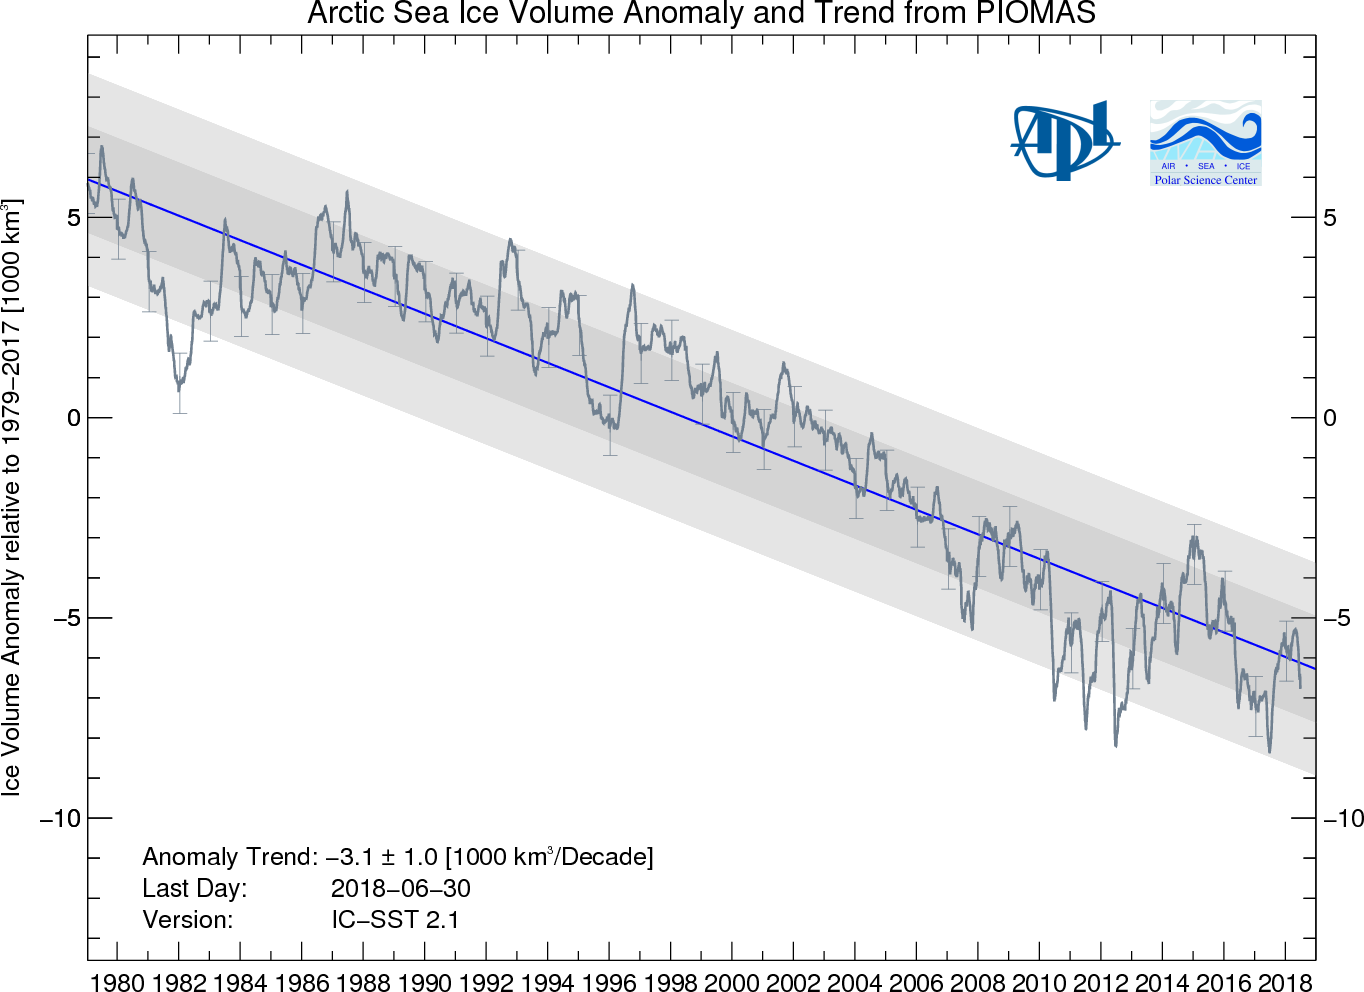
\includegraphics[width=1\linewidth]{src/images/chapter01/artic-sea-ice-volume.png}
\caption{Lines parallel to the regression line indicate Error Bound on the Observations\label{artic-sea-ice}}
\end{figure}
\typeout{************************************************}
\typeout{Exercises 1.10 Exercises}
\typeout{************************************************}
\subsection*{Exercises}\hypertarget{exercises-6}{}
\addcontentsline{toc}{subsection}{Exercises}
\begin{divisionexercise}{1}\hypertarget{exercise-15}{}
\hypertarget{p-137}{}%
As we will see in CHAPTER XX(5?), the error bands can be used with non-linear models as well.   Curves “parallel” to a function can be created by vertical shifts of the model up and down two standard deviations of the residuals. In the figure below, one and two standard deviations are shaded. Explain why the bands look wider in September than in June.%
\begin{figure}
\centering
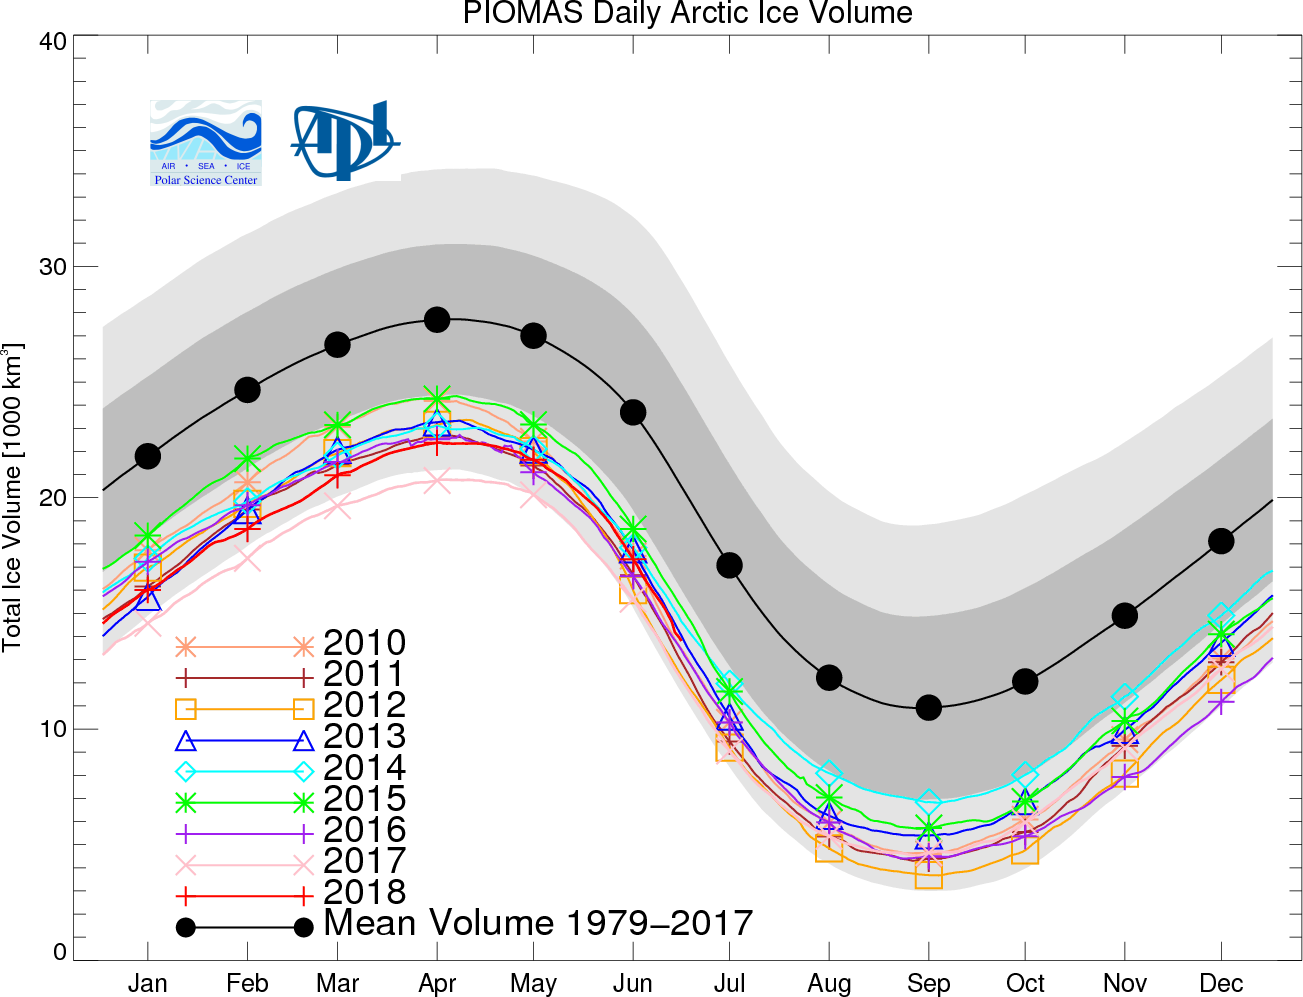
\includegraphics[width=1\linewidth]{src/images/chapter01/daily-artic-sea-ice-volume.png}
\caption{Yearly fluctuations in Arctic Ice Volume with 1 and 2 standard deviation curves highlighted.\label{figure-51}}
\end{figure}
\end{divisionexercise}%
\begin{divisionexercise}{2}\hypertarget{exercise-16}{}
\hypertarget{p-138}{}%
Calculate the error bounds for the Leaning Tower of Pisa data. Explain how you determined your error bounds.%
\end{divisionexercise}%
\begin{divisionexercise}{3}\hypertarget{exercise-17}{}
\hypertarget{p-139}{}%
A lumberjack has been studying the trees on the mountain beside his house. Last summer he measured the diameter of the trees at a height of \(1.2\) meters above the ground. He then used a tool to measure the height of the trees. The data he collected is given below:%
\begin{figure}
\centering
\begin{tabular}{cccccccc}
\multicolumn{1}{cC}{Diameter (cm)}&\(16\)&\(18\)&\(19\)&\(20\)&\(21\)&\(21\)&\(23\)\tabularnewline\hrulemedium
\multicolumn{1}{cC}{Height (m)}&\(12.9\)&\(13.2\)&\(12.8\)&\(15.0\)&\(15.7\)&\(14.9\)&\(14.7\)
\end{tabular}
 \begin{tabular}{cccccccc}
\multicolumn{1}{cC}{Diameter (cm)}&\(24\)&\(25\)&\(25\)&\(26\)&\(28\)&\(30\)&\(31\)\tabularnewline\hrulemedium
\multicolumn{1}{cC}{Height (m)}&\(17.3\)&\(19.2\)&\(15.2\)&\(18.6\)&\(17.9\)&\(16.4\)&\(19.5\)
\end{tabular}
\caption{Tree Data\label{figure-52}}
\end{figure}
\leavevmode%
\begin{enumerate}[label=(\alph*)]
\item\hypertarget{li-24}{}Make a scatterplot of the data, then find an equation of a line to fit this data.%
\item\hypertarget{li-25}{}If a tree has a diameter of \(36\) centimeters, what height does your equation predict?  Find error bounds.  How close should you expect your prediction to be?%
\item\hypertarget{li-26}{}If you know the diameter of a tree, based on your model above, is it likely that your prediction of the height of the tree will be within \(2\) meters of the actual height?%
\item\hypertarget{li-27}{}Use the linear equation that models the relationship between the diameter of the tree at \(1.2\) meters and the height of the tree to determine the equation of the linear model if the circumference had been used rather than the diameter. Which do you think the lumberjack actually measured, the diameter or the circumference? Is one measurement better to use than the other?  Explain your reasoning.%
\end{enumerate}
\end{divisionexercise}%
\begin{divisionexercise}{4}\hypertarget{exercise-18}{}
\hypertarget{p-140}{}%
Fit a line to the data you gathered in the experiments in SECTION XX. Describe the residual plot.  For those data sets that appear to be linear, find the error bounds. How confident are you in your model?%
\end{divisionexercise}%
\begin{divisionexercise}{5}\hypertarget{exercise-19}{}
\hypertarget{p-141}{}%
As we age, our vision deteriorates. A sample of \(30\) drivers had their vision tested to determine the distance they could identify a roadside sign. The equation of the regression line is \(y = -2.953x + 573.438\).%
\begin{figure}
\centering
{
\begin{tikzpicture}
  \begin{axis}[
    xlabel = {Age of Driver (yrs)},
    ylabel = {Distance Driver Could Identify Sign (ft) },
    ylabel near ticks,
    xlabel near ticks,
    xmin = 0, xmax = 90,
    xtick = {0, 10, ..., 80},
    ymin = 250, ymax = 650,
    ytick = {300, 350, ..., 600},
    axis y discontinuity=crunch,
    clip = false,
    restrict y to domain=0:700,
    ]

    \addplot[only marks, color=magenta] coordinates {
    (20, 588)
    (18, 508)
    (22, 557)
    (23, 508)
    (23, 458)
    (25, 488)
    (27, 557)
    (28, 508)
    (29, 458)
    (32, 411)
    (37, 419)
    (41, 459)
    (46, 448)
    (49, 381)
    (53, 459)
    (55, 420)
    (63, 349)
    (66, 300)
    (65, 420)
    (67, 412)
    (68, 302)
    (70, 390)
    (71, 321)
    (72, 369)
    (73, 281)
    (74, 420)
    (75, 460)
    (77, 361)
    (79, 312)
    (82, 361)

    };

    \addplot [thick, blue, <->, dashed, mark=none, domain=0:90,samples=200] {-2.953*x + 573.438} node[right] at (axis cs:35,500) {$ y = -2.953x + 573.438 $};

  \end{axis}
\end{tikzpicture}
}
\caption{Age (yrs) vs Distance (ft) at which driver could identify road sign\label{figure-53}}
\end{figure}
\hypertarget{p-142}{}%
\leavevmode%
\begin{enumerate}[label=(\alph*)]
\item\hypertarget{li-28}{}In what interval would it be unsurprising for a \(30\) year-old driver to recognize the sign?%
\item\hypertarget{li-29}{}A \(60\) year-old driver claims to be able to recognize the sign at \(500\) feet. Is this claim credible? Explain why or why not.%
\end{enumerate}
%
\end{divisionexercise}%
\end{document}